%\documentclass[12pt,draftcls]{ucdavisthesis}
\documentclass[12pt]{ucdavisthesis}

% PLEASE READ THE MANUAL - ucdavisthesis.pdf (in the package installation directory)

%%%%%%%%%%%%%%%%%%%%%%%%%%%%%%%%%%%%%%%%%%%%%%%%%%%%%%%%%%%%%%%%%%%%%%%%
%                                                                      %
%               LATEX COMMANDS FOR DOCUMENT SETUP                      %
%                                                                      %
%%%%%%%%%%%%%%%%%%%%%%%%%%%%%%%%%%%%%%%%%%%%%%%%%%%%%%%%%%%%%%%%%%%%%%%%

%\usepackage{bookmark}
\usepackage[us,nodayofweek,12hr]{datetime}
\usepackage{graphicx}
%\usepackage[square,comma,numbers,sort&compress]{natbib}
%\usepackage{hypernat}
% Other useful packages to try
\usepackage{amsmath}
\usepackage{amssymb}
\usepackage{accents}
\usepackage[]{algorithm2e}
\usepackage{caption}
\usepackage{subcaption}
%
% Different fonts to try (uncomment only fontenc and one font at a time)
% (you may need to install these first)
%\usepackage[T1]{fontenc} %enable fontenc package if using one of the fonts below
%\usepackage[adobe-utopia]{mathdesign}
%\usepackage{tgschola}
%\usepackage{tgbonum}
%\usepackage{tgpagella}
%\usepackage{tgtermes}
%\usepackage{fourier}
%\usepackage{fouriernc}
%\usepackage{kmath,kerkis}
%\usepackage{kpfonts}
%\usepackage[urw-garamond]{mathdesign}
%\usepackage[bitstream-charter]{mathdesign}
%\usepackage[sc]{mathpazo}
%\usepackage{mathptmx}
%\usepackage[varg]{txfonts}

\hyphenation{dis-ser-ta-tion blue-print man-u-script pre-par-ing} %add hyphenation rules for words TeX doesn't know


%\renewcommand{\rightmark}{\scriptsize A University of California Davis\ldots \hfill Rev.~\#1.0 \quad Compiled: \currenttime, \today}
% a fancier running header that can be used with draftcls options

%%%%%%%%%%%%%%%%%%%%%%%%%%%%%%%%%%%%%%%%%%%%%%%%%%%%%%%%%%%%%%%%%%%%%%%%
%                                                                      %
%        DOCUMENT SETUP AND INFORMATION FOR PRELIMINARY PAGES          %
%                                                                      %
%%%%%%%%%%%%%%%%%%%%%%%%%%%%%%%%%%%%%%%%%%%%%%%%%%%%%%%%%%%%%%%%%%%%%%%%

\title          {\textsc{A Polytopal Element Framework for\\
                 Improved Solution Accuracy and Robustness}}
%Exact title of your thesis. Indicate italics where necessary by underlining or using italics. Please capitalize the first letter of each word that would normally be capitalized in a title.

\author         {Brian Doran Giffin}
%Your full name as it appears on University records. Do not use initials.

\authordegrees  {B.S. (University of California, Davis) 2013 \\
                 M.S. (University of California, Davis) 2014}
%Indicate your previous degrees conferred.

\officialmajor  {\textsc{Civil and Environmental Engineering}}
%This is your official major as it appears on your University records.

\graduateprogram{Civil and Environmental Engineering}
%This is your official graduate program name. Used for UMI abstract.

\degreeyear     {2017}
% Indicate the year in which your degree will be officially conferred.

\degreemonth    {December}
% Indicate the month in which your degree will be officially conferred. Used for UMI abstract.

\committee{\textsc{Mark M. Rashid, Chair}}{\textsc{N. Sukumar}}{\textsc{Boris Jeremi\'{c}}}{}{}
% These are your committee members. The command accepts up to five committee members so be sure to have five sets of braces, even if there are empties.

%%%%%%%%%%%%%%%%%%%%%%%%%%%%%%%%%%%%%%%%%%%%%%%%%%%%%%%%%%%%%%%%%%%%%%%%

%\copyrightyear{2020}
%\nocopyright

%%%%%%%%%%%%%%%%%%%%%%%%%%%%%%%%%%%%%%%%%%%%%%%%%%%%%%%%%%%%%%%%%%%%%%%%

\dedication{\textsl{To Lyle \ldots \\
            for teaching me how to think deeply, to analyze new information objectively, and to appreciate the complexity and nuanced beauty in all things.} \\
            \textsl{And to Nancy \ldots \\
            for inspiring me to explore my creativity, for giving me canvases to paint on, and the confidence to paint, without fear of failure.}}

%%%%%%%%%%%%%%%%%%%%%%%%%%%%%%%%%%%%%%%%%%%%%%%%%%%%%%%%%%%%%%%%%%%%%%%%

\abstract{A high-level discussion of the fundamental problems accompanying finite element discretizations in the form of locking, addressing the scope of the work under consideration.}

%%%%%%%%%%%%%%%%%%%%%%%%%%%%%%%%%%%%%%%%%%%%%%%%%%%%%%%%%%%%%%%%%%%%%%%%

\acknowledgments{Many thanks to the following: Professor Amit Kanvinde who inspired much of my initial motivation for applying to graduate school; Professor N. Sukumar for exposing me to the realm of computational solid mechanics; Dr. Joseph Bishop at Sandia for being involved in my early (and continuing) development in the field of solid mechanics; Professor Mark Rashid who turned my spark of interest in the subject into a roaring fire of passion; Dr. Steven Wopschall and Mr. Omar Hafez for being my mentoring older brothers throughout my journey in graduate school; Mr. Subhajit Banerjee and Mr. Eric Chin whose fruitful discussions assisted greatly in developing a personal sense of calm and confidence prior to my qualifying examination; Professor Yannis Dafalias, Professor John Bolander, and Professor Elbridge Puckett, whose enthusiasm as lecturers and courtesy as QE examiners were indespensible; Dr. Joseph Jung, Dr. Kendall Pearson, Dr. Nathan Crane, Mr. Mark Merewether, Dr. Michael Tupek, and the whole of the Sierra Solid Mechanics Team at Sandia who introduced me to the fascinations of code development; Ms. Carly Arthur, Mr. Sam Mish, and Ms. Aim\'{e}e Sylvia whose conversations as fellow class-mates and advisees were incredibly helpful and insightful; and foremost to Ms. Maha Kenawy, who has served as my primary role-model and source of inspiration for completing this thesis -- I love you.}

%%%%%%%%%%%%%%%%%%%%%%%%%%%%%%%%%%%%%%%%%%%%%%%%%%%%%%%%%%%%%%%%%%%%%%%%

% Each chapter can be in its own file for easier editing and brought in with the \include command.
% Then use the \includeonly command to speed compilation when working on a particular chapter.
%%% \includeonly{ucdavisthesis_example_Chap1}

\begin{document}

\newcommand{\bibfont}{\singlespacing}
% need this command to keep single spacing in the bibliography when using natbib

\bibliographystyle{plain}
%many other bibliography styles are available (IEEEtran, mla, etc.). Use one appropriate for your field.

\makeintropages %Processes/produces the preliminary pages

\chapter{Introduction}

% OPENING (scope of the thesis)

	% A high-level description of the research setting:
		% Efficient & accurate approximation methods for nonlinear solid mechanics
	For decades, finite element methods (FEM) have been widely used by engineers and physicists in the modeling of solid continua. Numerous extensions of the method have been developed to model more complex physical processes, including large deformations and nonlinear material behavior.
	% A high% level statement of the fundamental problem(s):
		% FE solution accuracy is compromised by the issues of locking and mesh quality
		% Proposed solutions handle some, but not all of these problems
	In spite of these advances, traditional finite element methods have been plagued by recurrent issues of meshing, and numerical inaccuracies pertaining to locking and poor mesh quality. Various strategies have been proposed to overcome some of these issues, though few have been able to address them as a whole.
	
	% A high-level statement of the proposed solution(s):
		% Thesis presents a polytopal element framework to address these issues
		% Polyhedral discretization is aimed at overcoming issues of mesh quality
		% Framework is amenable to classical FE procedures used to address locking
	This thesis presents a novel polytopal element framework in an effort to address the collective issues of discretization sensitivity, and discretization, generally. The use of arbitrary polygonal and polyhedral shapes in place of canonical isoparametric elements seeks to resolve the issue of distortion sensitivity directly, obviating issues of meshing and mesh quality, while maintaining many of the desirable features of the FEM and its extensions.

\section{Historical Development} % (what has led up to polyhedral discretizations)

	% Origin of finite element methods, applied to solid mechanics problems
		% Finite elements developed initially for LINEAR, structural problems
	According to the historical account given by Felippa \cite{Felippa:04}, finite element methods originated in the 1950s to address engineering challenges in the design of aircraft, among other things. The method was subsequently given a more rigorous mathematical treatment by early contributors (Irons, Melosh, Strang), and its usage permeated to other fields of study (namely, structural engineering). Following the advent of the isoparametric element concept, displacement-based finite element formulations gained widespread popularity. Most early applications considered only small displacements and linear material behavior.
	% Subsequently, more complicated models were developed to accomodate nonlinearities:
		% Finite deformations incorporated to handle non-linear geometric effects
		% Advanced constitutive models developed for plastic and viscoelastic materials
		% Contact between deformable bodies (more geometric non-linearity)
	Subsequently, advanced solution methodologies were developed to accommodate various sources of nonlinearity, including finite deformations, nonlinear constitutive behavior, and contact.

	% Finite element methods still hold up in the aforementioned contexts because:
		% Compact support property of basis functions yields efficient solutions
			% Domain decomposition more straightforward, parallel scalability
		% Element quadrature rules effectively consider individual material points
			% leads to reasonable accuracy and solution efficiency
			% directly compatible with the theory of continuum mechanics
			% naturally accomodates non-linear kinematics
			% naturally accomodates non-linear constitutive models
		% Yields a precise description of mesh boundaries
			% allows for straightforward contact enforcement
			% application of other BC's (FSI pressure coupling) also straightforward
	Over half a century after its initial development, the finite element method is still widely used, and recognized as the industry standard technology for modeling complicated structural and dynamic systems. Its reigning popularity can be attributed to several desirable features of the method:
	\begin{itemize}
		\item The compact support property of the isoparametric basis functions helps to facilitate more efficient solution methodologies. In particular, the assembly of finite element systems of equations is rendered more efficient (and modular) by an element-wise assembly process.
		\item The Kronecker delta property and precise description of mesh boundaries allow for a relatively straightforward application of boundary conditions and contact constraints.
		\item Numerical quadrature on element domains derived from product Gauss rules balances accuracy, efficiency, and stability. Domain quadrature rules also naturally accommodate nonlinear kinematic behavior and ``black box'' constitutive models.
	\end{itemize}	
	
	% However, finite element methods have suffered from two major (but related) issues:
		% Poor solution accuracy due to effects of ``locking''
			% The quality and type of discretization heavily impacts accuracy
			% Low order elements suffer the most from these issues
			% Linear tetrahedra and triangles are the worst offenders
			% Thin an distorted elements perform poorly
		% Meshing of complex geometries into quality discretizations is difficult
			% Generally time-consuming to produce quality meshes (human effort)
			% Hard or impossible to avoid mesh distortion
			% Recent developments have been made towards hex-dominant meshing
				% still limited by element distortion
	However, despite these advantageous characteristics, finite element methods have suffered from two major (related) issues:
	\begin{itemize}
		\item[I.)] Standard element formulations are prone to the effects of numerical locking phenomena, which can significantly degrade the accuracy of the method. These issues are more prevalent for low-order elements, especially for linear triangles and tetrahedra. Moreover, very thin or distorted elements tend to exhibit more severe pathologies.
		\item[II.)] The process of discretizing complex geometries into traditional finite element shapes is not always possible with current automated meshing techniques. Contemporary meshing tools typically require extensive human intervention to produce meshes for complex shapes. This process is further encumbered by the aforementioned concerns over locking, to the extent that it becomes difficult -- if not impossible -- to produce quality discretizations within a reasonable amount of time. To compound this problem, the issue of re-meshing for problems involving severe plastic deformations presents a major challenge for Lagrangian approaches \cite{Hattangady:99}.
	\end{itemize}
	
	Blacker \cite{Blacker:00} presents a comprehensive overview of the issues pertaining to meshing, and Owen \cite{Owen:14} provides a survey of several meshing technologies in common usage. An updated overview of several new methods for automated hexahedral meshing may be found in \cite{Staten:07}. In recent years, numerous efforts have sought to improve upon these existing techniques. Owen and Shelton \cite{Owen:14} have demonstrated improvements in solution accuracy through the use of an automated mesh ``sculpting'' procedure. Qian and Zhang \cite{Qian:12} have made advancements toward the generation of conforming meshes for complex part assemblies. Kremer et al. \cite{Kremer:14} have investigated a novel technique for generating all-hexahedral meshes from quad surface meshes. Recent efforts to pursue automated quad-dominant \cite{Remacle:12} and hex-dominant \cite{Xifeng:17} meshing algorithms have also gained increasing attention. Despite these advances, few -- if any -- of the aforementioned approaches are capable generating quality meshes for truly arbitrary geometries.
	
	Even with the advent of new hexahedral-dominant meshing technologies, however, the inherent problems of locking and distortion sensitivity still limit the solution accuracy of traditional isoparametric elements. Consequently, substantial efforts have been made to address the locking problem through a variety of approaches. An overview of locking and its remedies is given in the following section.

	\subsection*{Locking in Finite Elements}
	
		% Establish fundamentally what locking is
			% observations regarding volumetric locking
			% observations regarding shear locking
			% mathematical characterization of locking by Babuska
		Locking, as a general phenomenon \cite{Babuska&Suri:92:1}, is characterized by a drastic loss of solution accuracy and/or convergence for particular choices of material or discretization parameters. In mathematical terms, an approximation method is deemed \textit{robust} (with respect to a given problem parameter) if its numerical solution converges ``uniformly'' to the exact solution under mesh refinement, for all values of the indicated problem parameter. Conversely, a method is said to exhibit \textit{locking} if the accuracy of the numerical solution degenerates as the chosen problem parameter approaches some limiting value.
		
		As a specific example, one of the most commonly discussed and addressed forms of locking in computational solid mechanics is the issue of \textit{volumetric locking}, wherein displacement-based element formulations suffer from a marked loss of accuracy when utilized to model the deformation of nearly incompressible materials. For an isotropic linear elastic material model, the parameter dependency in question relates to the Poisson's ratio of the material.
		
		Other forms of locking may manifest as a sensitivity to geometric/discretization parameters. These are collectively referred to as \textit{geometric locking} phenomena, which include: \textit{shear locking}, which is linked to the aspect ratio of continuum elements subjected to bending-dominated deformations; \textit{membrane locking}, which occurs in curved shell elements (see \cite{Winkler:10}); and \textit{trapezoidal locking}, which affects the bending response of distorted four-node quadrilateral elements (see \cite{MacNeal:87}).
	
		% Concerted efforts were made to address the issues of locking:
		
		% Higher-order elements
			% shown to eliminate locking issues at high enough order
			% accuracy still highly contingent on element distortion
			% complexity of high-order elements seen as disadvantageous
		Early efforts to address locking sought to develop more robust discretizations through the use of higher-order elements. In \cite{Babuska&Suri:92:2} and \cite{Suri:91}, Babu\u{s}ka and Suri rationalized the ability of high-order elements to overcome the effects of volumetric locking (for triangular discretizations). The improved convergence behavior of these elements made them an attractive option for seeking efficiency gains, as well. Nonetheless, higher-order elements were generally seen as too complex in comparison with the standard low-order elements commonly used for commercial applications. For example, many cite the relative difficulty of obtaining lumped mass matrices for high-order elements \cite{Hughes:00}. Moreover, the accuracy of high-order isoparametric elements can be severely degraded if the elements possess curved edges \cite{Lee&Bathe:93}.
			
		% Mixed formulations based on Hu-Washizu principle
			% one of the most robust solutions to locking
			% directed at incompressibility, resolves pressure field accurately
			% requires the interpolation of displacement, strain, and stress fields
			% must satisfy the inf-sup (LBB) conditions for stability
			% somewhat limited, based on the choice for the material model
			% can suffer from issues of numerical conditioning
		As an alternative to the standard displacement-based FEM, some have argued for the use of \textit{mixed finite element methods} (MFEM), which provide, in the most general case, a separate interpolation of the displacement, strain, and stress fields. Mixed methods are derived from a 3-field Hu-Washizu variational principle in the specification of the weak form. While these methods are generally less vulnerable to locking (as noted in \cite{Babuska&Suri:92:2} and \cite{Babuska&Suri:92:1}), they are not altogether immune to its effects. Moreover, mixed methods are subject to potential issues of stability, i.e. the Babu\u{s}ka-Brezzi -- or inf-sup -- conditions (\cite{Babuska:71}, \cite{Brezzi:74}.) Additionally, mixed methods tend to be less efficient in comparison with displacement-based FEM, and are not as flexible in their ability to handle arbitrary constitutive relationships.
		
		% Method of incompatible modes
			% aimed mostly at improving bending performance of elements
			% based on mixed formulations, reduced to 2-field method
			% considers enhanced strain mode degrees of freedom
			% enhanced dofs can be condensed out at the element level
			% performance of elements is still sensitive to mesh distortion
		In an effort to retain some of the beneficial characteristics of mixed finite element methods, \textit{(mixed) assumed strain methods} were formalized for geometrically linear problems in \cite{Simo&Rifai:90}, and extended to nonlinear problems in \cite{Simo&Armero:92} and \cite{Simo&Armero&Taylor:93}. Assumed strain methods are closely related to the \textit{method of incompatible modes} first proposed by Wilson \cite{Wilson:73}, which considers the inclusion of additional element-specific modes of deformation that allow for discontinuities in the resulting displacement field at element boundaries. By contrast, assumed strain methods are derived from a 3-field variational principle, and rely upon energy orthogonality between an enhanced strain field and the resulting stress field to eliminate the need for an independent stress interpolation space. Assumed strain methods may therefore be viewed as as a class of mixed 2-field formulations, involving a compatible displacement field and an enhanced/assumed strain field. Though the method is effective in treating a variety of geometric locking phenomena, it nonetheless leads to spurious instabilities in both linear and nonlinear problems (see \cite{Bathe&Sussman:14} and \cite{Bathe&Pantuso:97}, respectively), even for element formulations satisfying the inf-sup conditions.
			
		% Selective Reduced Integration techniques
			% developed to handle incompressibility constraint
			% works fairly well, though may fail inf-sup
		Other attempts to adapt mixed formulations for more general use with arbitrary material models without relying upon an explicit interpolation of the stress or strain fields include \textit{selective reduced integration} (SRI) and equivalent \textit{strain projection} techniques. These methods were fairly successful in overcoming the issues of volumetric locking via the B-bar projection approach for linear problems discussed in \cite{Hughes:00}, and via the F-bar approach for nonlinear problems discussed in \cite{Souza:96}. Though these methods can be both effective and efficient, their success has been limited to the problem of volumetric locking; they are somewhat less successful with regard to treating other forms of locking, such as shear locking in continuum finite elements \cite{Malkus&Hughes:78}. SRI can also lead to stability problems if the strain projection spaces are not selected carefully.
		
		% Hourglass stiffness and viscosity
			% use underintegration of the element (single point quadrature)
			% supplement with (small) artificial stiffness & viscosity parameters
			% efficient computationally, especially for explicit dynamics
			% an ad hoc solution, sensitive to the choice of HG parameters
		At the opposite end of the spectrum -- in recognition of the inherent issues of stability plaguing mixed methods and reduced integration techniques, methodologies employing \textit{orthogonal hourglass control} have been suggested \cite{Flanagan:81}. These approaches consider the use of low-order quadrature rules to avoid common locking phenomena, supplemented by artificial stiffness terms to maintain stability while preserving essential convergence characteristics. While these formulations tend to be highly efficient computationally (particularly for explicit dynamics), the obvious disadvantage of these approaches relates to their reliance upon user-specified artificial stiffness and viscosity parameters. Appropriate selection of these parameters is not always a trivial matter, and often warrants problem-specific investigations via sensitivity analyses.
			
		% Important point: most of these methods restricted to standard (hex) elements
			% not easily generalizable/extensible to other elements/methods
			% moreover, standard isoparametric elements are part of the problem
				% led to development of alternative methods/discretizations
		Ultimately, the foregoing methodologies have had only limited success in resolving the full spectrum of locking problems, particularly with regard to geometric locking phenomena. Moreover, many of the proposed enhancements are limited to specific element types (typically low-order quadrilaterals or hexahedra), and are not readily generalizable to other discretizations.
		
		On the whole, the approximating power of the FEM is controlled to a lesser extent by the accuracy of the numerical integration rules used, and to a much greater extent by its ability to adequately represent smooth solutions over individual elements (or patches of elements). Local polynomial reproducibility ultimately determines the ``approximability'' of a given function space, with loss of polynomial completeness leading to a corresponding loss of accuracy and convergence. In the case of isoparametric elements, non-affine distortions may severely impact the polynomial completeness of certain element types \cite{Lee&Bathe:93}. However, even elements which retain polynomial completeness may still lose accuracy/convergence in certain configurations, such as when the elements possess sufficiently large interior angles \cite{Acosta:00}. For this reason, considerable efforts have been invested in recent years towards the development of alternative discretizations and numerical methods, a few of which are discussed in the following section.
		
		% Say something about how accuracy is controlled by loss of completeness, integration consistency. 
		
		%To a large extent, the propensity for locking in FEM is controlled by the standard isoparametric elements' sensitivity to geometric distortion. In other words, model accuracy is too often the product of the chosen discretization. For this reason, considerable efforts have been invested in recent years towards the development of alternative discretizations and numerical methods, a few of which are discussed in the following section.
	
	\subsection*{Alternative Numerical Methods and Discretizations}
		% Efforts toward meshing & element quality led to new methods & discretizations
		Driven primarily by concerns over meshing (and additionally by concerns over element quality), a variety of alternative approximation methods have been developed in recent decades. Such methods admit more general discretizations and approximation spaces in an effort to circumvent problems pertaining to conforming finite element mesh generation.
		
		 %The general consensus is that the construction of an approximation space should be disconnected (to a variable extent) from the particular choice of discretization. In particular, isoparametric finite element basis functions are conveniently defined in terms of the discretization, but may not necessarily result in a suitable approximation space for the given problem at hand.
		
		% Say something about how we should like to define approximation spaces in a more flexible way. Additionally, consider the fact that these methods are intended/aimed at avoiding the meshing problem altogether. (Mesh-free methods, in particular, are driven by the desire to avoid having to create a mesh in the first place; not by element quality.)
		
		% Meshfree methods
			% avoid issues of mesh sensitivity altogether -- abandon the mesh
			% construct shape functions using weighting/kernal functions
			% several different varieties: SPH, MLS, RKPM, Max-Ent
			% solutions tend to be much smoother
			% able to handle severe/extreme deformations & changing topology
			% lose compact support property; less computationally efficient
			% boundaries are not well-defined; handling of BCs and contact is hard
			% suffers from issues of numerical integration; lose consistency
			% need to define a background mesh for integration (NOT mesh-free)
		In direct response to the concerns over meshing, so-called \textit{mesh-free} methods were developed in an effort to construct approximation spaces that are defined with reference to an arbitrary collection of points, rather than a finite element partition of the domain. Mesh-free methods encompass a broad class of approximation schemes. For solid mechanics applications, these include: smoothed particle hydrodynamics \cite{Libersky:91}, the element-free Galerkin method \cite{Belytschko:94}, the natural element method \cite{Sukumar:98}, and the reproducing kernel particle method \cite{Liu:95}, among others. A majority of these methods rely upon an \textit{a priori} specification of weighting functions used to construct an associated set of polynomially reproducing basis functions. The resulting mesh-free bases yield smooth solutions, which are relatively insensitive to the specific choice and distribution of weighting kernels.
		
		% fix: specific choice and distribution of weighting functions
		
		The departure from defining an approximation space on a partition of the domain presents a number of challenges, however. Specifically, mesh-free methods still require the definition of a background mesh to effect numerical integration of the weak form, partially invalidating the namesake of the method. Nodal integration techniques have been suggested to partially overcome this issue \cite{Beissel:96}, though such schemes are generally susceptible to numerical instabilities. Stabilized nodal integration methods have been developed in response to these problems (\cite{Chen:01}, \cite{Chen:07}). Nonetheless, because the mesh-free basis functions are typically non-polynomial in form (and because their supports are not aligned with the integration cells), integration errors may result in loss of polynomial consistency and solution accuracy. Chen et al. have proposed a means of overcoming these issues through a \textit{variationally consistent integration} scheme \cite{Chen:13}, which is generally applicable to background integration and nodal integration techniques, alike.

		% Discuss nodal integration methods, issues of stability, etc.
		
		% Shepard? Sherman?
		
		Because the mesh-free basis functions will not necessarily exhibit the Kronecker delta property, the application of essential boundary conditions and contact constraints becomes less straightforward. Several techniques have been proposed to address this issue \cite{Mendez:04}, including Lagrange multiplier methods, Nitsche's method, and mesh blending at domain boundaries.
			
		% Discontinuous Galerkin methods
			% accomodate arbitrary polytopal domains
			% solution within a given polytopal domain is locally polynomial
			% tends to be fairly robust across different discretizations
			% relatively efficient, shares some favorable characteristics of FEM
			% penalty terms are needed to enforce BCs & weak continuity
			% penalty parameters are problem dependent, must be chosen carefully
		As another alternative, \textit{discontinuous Galerkin} (DG) methods have gained recent attention due to their more flexible representation of solution fields as piecewise polynomials over individual elements, resulting in solution discontinuities at element boundaries. To stabilize the resulting approximation space, DG methods supplement the weak form with interior penalty terms that seek to minimize these discontinuities. A detailed review of several primal interior penalty DG schemes may be found in \cite{Riviere:08}. DG methods are advantageous in that they may accommodate arbitrary element shapes, and exhibit desirable distortion robustness characteristics.
		
		DG approaches are not without their own problems, however. One commonly cited issue relates to the fact that DG methods can become sensitive to the choice of penalty parameters used to weakly enforce inter-element continuity and boundary conditions. Indeed, the selection of these parameters is problem dependent. Additionally, DG methods tend to suffer from poor numerical conditioning problems if the discretization does not conform to relatively stringent regularity requirements \cite{Mu:14} (element edges cannot be too small), thereby limiting the types of discretizations used with the method.
		
		% Add reference to regularity requirements of elements.
			
		% Weak Galerkin methods
			% more recently developed approach
			% can handle arbitrary polytopal element domains
			% based on the notion of weak derivatives
			% similar in some respects to DG methods; polynomial basis functions
			% dofs stored in element domains, and on element boundaries
			% weak derivative property avoids need for penalty terms (unlike DG)
			% may result in a large number of unknowns, less efficient
			% current formulations place limits on element geometry			
		
		The more recent \textit{weak Galerkin} (WG) finite element method first introduced by Wang and Ye for elliptic problems in \cite{Wang:13}, and for parabolic equations by Li and Wang in \cite{Li:13}, pursues the discretization of a (2D) problem domain into polygonal elements and element edges. The method considers a space of ``weak functions'' defined independently on element interiors and their boundaries, such that for any function $v = \left\{ v|_\Omega, \, v|_{\partial \Omega} \right\}$, its (discrete) ``weak gradient'' $\nabla_{\mathrm w,k} \, v \in V(\Omega,k)$ is defined on the interior of a given element $\Omega \subset \mathbb{R}^d$ through its action on a vector field $\bm{q} \in V(\Omega,k)$:
\begin{equation}
	\int_\Omega \bm{q} \cdot \nabla_{\mathrm w,k} \, v \, \mathrm dA = - \int_\Omega v|_\Omega \nabla \cdot \bm{q} \, \mathrm dA + \int_{\partial \Omega} v|_{\partial \Omega} \, \bm{q} \cdot \bm{n} \, \mathrm dS, \quad \forall \bm{q} \in V(\Omega,k),
\end{equation}
where $V(K,k) \subset \left[ P^k (\Omega) \right]^d$ is a subspace of the vector-valued polynomials of maximal degree $k$ defined on $\Omega$. A weak Galerkin approximation method uses the discrete weak gradient operator in place of the classical gradient.

	The discrete approximation spaces under consideration are typically low-order polynomials (commonly just constants) defined on the elements and their edges. However, there are some non-trivial choices that must be made regarding an optimal selection of these polynomial spaces for the sake of computational efficiency (discussed in greater detail in reference \cite{Mu:15:1}). The method has so-far only been applied to the solution of linear problems.

	The computational accuracy of the weak Galerkin approach has been explored by Mu et. al. in \cite{Mu:13}, showing that for certain problems, the weak Galerkin method converges at rates comparable to those of the standard FEM. Lin et. al. performed a comparative study between the weak Galerkin, discontinuous Galerkin, and mixed finite element methods in \cite{Lin:15}, demonstrating some of the competitive and desirable characteristics of WG in contrast to DG or MFEMs: no need for penalty parameters, and definiteness of the resulting linear system of equations.

	Mu et. al. adapted the method for use on arbitrary polytopal meshes in \cite{Mu:15:2} and \cite{Mu:15:1}, albeit with a number of shape regularity restrictions placed on the elements. In general, the implementation of WG considers the mesh degrees of freedom as belonging to both the elements and their edges, however in \cite{Mu:15:1} it is noted that the local element degrees of freedom can be expressed in terms of the bounding edge degrees of freedom alone, to improve computational efficiency. A modified approach by Wang et. al. in \cite{Wang:14} instead chooses to express functions on edges only implicitly. Although this approach successfully eliminates the computational expense associated with edge-based degrees of freedom, it requires the inclusion of an additional interior penalty term in the weak form, similar to a discontinuous Galerkin method.

	% Polygonal and Polyhedral methods
		% element geometry made to be more flexible (arbitrary)
			% opens up new possibilities for meshing
		% construct basis functions directly on the elements (no isoparametric map)
		% basis functions possess compact support; numerically efficient
		% mesh boundaries again well-defined; good for contact & BC enforcement
		% techniques developed for efficient domain integration (Sukumar, Mousavi)
	In the wake of these investigations, it becomes clear that the combination of desirable properties held by the FEM (compact support, Kronecker delta, quadrature efficiency, DoF efficiency, stability, and inter-element compatibility) are qualities worth preserving. To this end, recent efforts within the numerical methods development community have focused on improving and generalizing existing element formulations for arbitrary element shapes -- polygons and polyhedra. Rather than relying upon shape functions defined through an isoparametric transformation from a parent element domain, recent polytopal element methodologies have explored various techniques for constructing approximants directly on physical element domains. In doing so, issues regarding distortion sensitivity of the elements are largely obviated, and new opportunities for discretizing the domain with irregular shapes are made possible.
	% New discretization methods have made polyhedral meshing more accessible
		% Voronoi meshing has made leaps and bounds in recent years (Ebeida)
		% Efforts made toward hex mesh intersection with B-rep geometry (Celeris)
	In like fashion, recent advances in meshing technologies have made polyhedral element methods a readily feasible option. Very recently, Ebeida et. al. have released VoroCrust \cite{Ebeida:17}: a robust Voronoi discretization tool based on constrained Poisson disk sampling. Concurrent technologies have also advanced polyhedral mesh generation via boolean intersection of a background hexahedral mesh with a piecewise linear boundary representation (or B-rep).

	% Justify current demand for reliable and robust polyhedral element methods
	For these reasons, efficient and robust polyhedral element formulations are in high demand, leading to a proliferation of new approaches. A number of these are discussed in the following section.

\section{Recent Advances in Polytopal Element Methods} % (polyhedral finite element methods)

	% Reiterate the main motivation behind polyhedral discretizations
		% Want to avoid meshing limitations while preserving desirable FEM properties
			% definition of quadrature rules & precise boundary description
	Polytopal element methods combine many of the attractive features of FEM with the geometric flexibility afforded by arbitrary element shapes, the primary motivation for which arises from the aforementioned concerns over meshing and discretization sensitivity. Most of these methods share a few distinguishing features in common with one another: mesh degrees of freedom are borne by nodes -- the geometric vertices of (low-order) elements; nodal basis functions are compactly supported over adjoining element domains, and satisfy the Kronecker delta property; basis functions are defined directly on the element's physical domain, rather than on a parent domain.
	
	% Discuss meshing problem more!
	
	Where these methods differ is in the way that they choose to define an element's shape functions (if at all). These approaches may be loosely organized into three distinct categories: methods which explicitly define the element's basis functions via a continuous interpolation scheme; methods which define the element's shape functions only implicitly -- i.e. ``virtual'' element methods; and methods which form a discrete representation of the element's shape functions via an approximation scheme. These three methodologies are elaborated upon in the following sections.

	\subsection*{Continuous Interpolation on Arbitrary Polytopes}
		% Overview of efforts to define interpolants directly on polytopal domains
		A key advantage of isoparametric elements relates to their straight-forward, point-wise definition of an element's shape functions. In an effort to preserve this desirable characteristic, various authors have sought to explicitly define shape functions directly on arbitrary polytopal element domains. These efforts have led to the creation of a broad family of interpolation schemes, collectively referred to as \textit{generalized barycentric coordinates} \cite{Sukumar:17}.
		
		% Briefly describe the idea of generalized barycentric coordinates
			% harmonic/Laplace coordinates
			% Waschpress coordinates
			% maximum entropy coordinates
		At a minimum, shape functions which fall into this category must: form a partition of unity, satisfy linear completeness, and interpolate the nodal data (i.e. satisfy the Kronecker delta property). These coordinates are uniquely defined according to the standard barycentric coordinate system for simplicial domains. For arbitrary polytopal domains, numerous such coordinate systems exist, including Wachspress' coordinates \cite{Wachspress:75}, mean value coordinates \cite{Floater:03}, harmonic coordinates \cite{Joshi:07}, and maximum entropy coordinates \cite{Sukumar:04}, among others. In many cases, such coordinates are restricted to strictly convex polytopes.
			
		% Require significant number of quadrature points to retain accuracy
		Though generalized barycentric coordinates have been applied in the context of finite elements, their development has largely been propelled by the graphics community on account of their relatively smooth interpolatory properties. However, the smooth (non-polynomial) character of the shape functions presents a challenge with regard to accurate numerical integration. Consequently, relatively high-order quadrature schemes are required to achieve reasonable solution accuracy and satisfaction of patch tests. More recently, a polynomial projection scheme has been suggested in \cite{Talischi:14} to remedy these integration errors for linear problems; for general nonlinear problems, a gradient correction scheme has been proposed in \cite{Talischi:15} and \cite{Chi:16}. These developments have illuminated new possibilities for defining more efficient quadrature rules on polytopes, while still satisfying the essential requirements for convergence.
		
		% Many approaches are limited by restrictions on element geometry/convexity
		Yet in spite of these developments, many existing coordinate schemes are sill limited by moderate to severe restrictions on element shape/convexity, and produce sharp gradients in the presence of degenerate geometric features. These concerns, and a recognition of the fact that the shape functions need not be defined point-wise for finite element applications, have motivated research efforts toward discrete representations of element interpolants.

	\subsection*{Virtual Element Methods}
		% Overview of virtual element methods (avoids definition of SFs on element domains)
		% never explicitly constructs/represents shape functions on elements
		% considers ``virtual'' shape functions, projected onto a polynomial subspace
		% exploits linearity of bilinear form to separate consistency & stability terms
		% consistency term formed by low-order polynomial projection of virtual SFs
		% stability term formed by higher-order projection, scaled by HG parameter
		% limited in applicability to linear problems (some efforts toward nonlinear)
		% stabilization still a somewhat ad hoc procedure
		The \textit{virtual element method} (VEM) summarized in \cite{Veiga:13} is a relatively new approach, based in part upon the older concept of mimetic finite differences (MFD). Although the method supposes that continuous basis functions \textit{exist} within arbitrary polytopal elements, the VEM never explicitly \textit{defines} how these shape functions vary on element interiors. Instead, the VEM supposes that these ``virtual'' functions may be separated (via projection operators) into polynomial and non-polynomial parts, which are handled in different ways. The cornerstone of the method is the idea that the bilinear form for a given element may be decomposed into two distinct parts: a term which guarantees variational consistency (Galerkin exactness) involving the low-order polynomial part of the shape functions, and a term which provides stability involving the non-polynomial part. The consistency term must be integrated exactly, but the stability term can be evaluated approximately. Because this decomposition relies upon the linearity of the bilinear form, direct generalizations of the method to nonlinear problems are not immediately available.
		
		VEM has been applied to three-dimensional linear elasticity problems in \cite{Gain:13}. In \cite{Veiga:15}, a VEM formulation for low-order elements which accommodates nonlinear ``black-box'' constitutive algorithms is presented, and in \cite{Chi:17} an extension to finite deformations (with appropriate stabilization terms) is introduced. Given the means by which these approaches exploit the use of a projected uniform gradient to integrate the weak form, however, it is unclear how they could be extended to accommodate higher-order elements.
		
		Nonetheless, VEM formulations are able to tolerate geometric degeneracies and element non-convexity without encountering serious numerical difficulties, though their good behavior in the presence of these features is often governed by an ad hoc approximation of the stabilization terms. A more rigorous development of the corresponding stability terms for more complicated element domains remains to be explored.
		
	\subsection*{Approximate Interpolation on Arbitrary Polytopes}
		% Overview of efforts to define shape functions only loosely over element domains
		% Somewhere in between the barycentric coordinate-type elements, and the VEM
		In contrast with the previously described approaches, yet another strategy considers the representation of the element's shape functions in an approximate way, while enforcing a few essential requirements, namely: polynomial reproducibility, inter-element compatibility, and weak form consistency.
		
		% VETFEM (variable element topology finite element method)
			% define SFs as polynomials, subject to continuity requirements
			% suffers from robustness issues
		In \cite{Rashid:00} and \cite{Rashid:06}, Rashid and co-workers  explored the \textit{variable element topology finite element method} (VETFEM), characterized by an approximate representation of the element's shape functions as low-order polynomials satisfying weak continuity requirements at element boundaries. Within this framework, the element shape functions are determined by a local minimization problem, resulting in polynomial shape functions which optimize specified continuity and smoothness objectives. This minimization procedure is constrained by the requirements of consistency and reproducibility to guarantee satisfaction of linear patch tests. Dohrmann and Rashid later extended this approach to higher-order elements in \cite{Dohrmann:02}, instead focusing on a direct construction of shape function derivatives, rather than of the shape functions themselves.
		
		The VETFEM may be viewed as a non-conforming finite element method, as the minimization process altogether allows for residual discontinuities at inter-element boundaries. Nonetheless, because the elements satisfy weak continuity requirements, the method exhibits proper convergence characteristics. Additionally, because the VETFEM yields a point-wise representation of the shape functions as low-order polynomials, direct integration of the weak form can be carried out using relatively efficient domain quadrature rules.
			
		% DDPFEM (discrete data polyhedral finite element method)
			% define only SF values and gradients at discrete points
			% requires a partition of the element into cells
			% element formulation more robust with finer partition
		Although the VETFEM was developed to handle arbitrary polygonal elements, it was observed to suffer from sensitivity to geometric degeneracies and element non-convexity. In response to these issues, a \textit{discrete data polyhedral finite element method} (DDPFEM) proposed in \cite{Selimotic:08} was suggested to exploit the fact that for typical solid mechanics applications, it is generally only necessary to evaluate the element's shape functions (and their derivatives) at a discrete number of quadrature points. The proposed method shares several characteristics in common with the VETFEM, utilizing a similarly posed constrained minimization procedure to obtain the precise values and gradients of the shape functions at discrete points within a given element. One of the cited challenges with this approach pertains to the appropriate selection of an efficient quadrature rule for the elements.
			
		% PEM (partitioned element method)
			% embraces element partition idea
			% construct SFs in hierarchial manner, assume SFs piecewise polynomial
		Nonetheless, the initial thoughts put forward by the DDPFEM ultimately led to the development of the \textit{partitioned element method} (PEM) presented in \cite{Rashid:12}. The PEM proceeds by partitioning an element into polygonal quadrature cells, and allowing the element's shape functions to vary according to a local polynomial defined within each of these cells, resulting in piecewise polynomial shape functions which are discontinuous at quadrature cell boundaries. The polynomial coefficients defined in each cell are obtained by minimizing the discontinuities in the shape functions across all cell interfaces, subject to the necessary consistency and reproducibility constraints. The original presentation in \cite{Rashid:12} considers the shape functions to be approximate solutions of Laplace's equation on the partitioned element. Later developments have dispensed with this supposition, instead only penalizing discontinuities in the shape functions (and their gradients) at cell boundaries.
			
		% Joe Bishop's version of FE-based approximants w/ Laplace shape functions
			% similar in concept: discretize element domain
			% use FE basis functions on a local tet mesh, solve Laplace equation
		Subsequently, Bishop has proposed a very similar partitioned element scheme in \cite{Bishop:14}, wherein the elements and their faces are subdivided into simplices, resembling a local FE discretization of the element domain. The shape functions are obtained as the solution to Laplace's equation on this subdivision. Because this approach utilizes an FE-like discretization, the resulting shape functions are piecewise linear and $C^0$ continuous, thereby avoiding the need for a penalty term to enforce continuity. However, the method still requires the use of a gradient correction scheme to account for quadrature error and thereby recover consistency with the weak form.

	% Lead into the present work, following last category: ``partitioned element methods''
		% select the PEM approach as the one of particular interest for this thesis
	In light of these developments, we choose to recognize a new class of methods, herein collectively referred to as \textit{partitioned element methods}. These may be viewed as a generalization of the original approach presented in \cite{Rashid:12}. It is the subject of this thesis to further explore these methods, and to expose their particular merits and potential shortcomings.

\section{Scope of the Present Work}

	% Description of the partitioned element framework
		% Elements are discretized (partitioned) into cells (atomic units of mesh)
		% Approximation space is constructed on this partition (much like FE, etc.)
		% A local BVP is solved to obtain shape functions on the partition
		% Solution method depends on choice of local approximation method; many choices
		% Quadrature rules on the element are informed by the partition
	In this work, a general framework for \textit{partitioned element methods} (PEM) is established, constituting a family of approaches for constructing piecewise polynomial approximations to harmonic shape functions on arbitrary polytopes. Numerous approaches may be developed within this framework, though only a handful are explored in detail within the scope of this dissertation.
	
	% Assert that nonlinearities (material & kinematic) are accomodated in this framework
	% Describe how this framework can accomodate standard anti% locking formulations
		% Allude to the incorporation of these methods as part of present research
	 The partitioned element methods developed herein are intended for applications in nonlinear solid mechanics. The efficacy of these methods will be assessed with regard to their ability to accommodate large deformations and nonlinear material behavior. The robustness of each method with respect to element shape, and its performance in the face of locking phenomena will be examined.
	 
	 % Additionally, several methodologies which leverage the partitioned element framework to combat certain forms of locking will be discussed.
	 
\subsection*{Original Contributions}

	While the ideas which underpin partitioned element methods have already appeared in the literature (\cite{Rashid:12}, \cite{Bishop:14}), this work presents a unification of such concepts within a common framework. An original analysis of these approaches with regard to their ability to recover integration consistency is presented in chapter \ref{ch:pem}.
	
	The \textit{discontinuous Galerkin partitioned-element method} (DG-PEM) constitutes the most substantial contribution presented herein. It's mathematical formulation, analysis, implementation, and numerical investigation represent the sole work of the author.
	
	The numerical investigations considered in chapter \ref{ch:results} were performed using the Fortran-based solid mechanics code entitled ``Machina.'' This program was written and tested exclusively by the author (with the exception of the linear solver package \cite{Davis:04}).
	
	A novel, and highly accurate incremental kinematics algorithm for rate-based constitutive models was utilized for all problems in chapter \ref{ch:results} which involved finite deformations. A brief, contextual allusion to this algorithm is given in chapter \ref{ch:solid_mechanics}, with a more detailed explanation intended in a forthcoming publication \cite{kinematics_paper}.
	
	A novel analytical solution for the incompressible twisting annulus verification problem considered in chapter \ref{ch:results} is derived in the Appendix.

\subsection*{Organization}	

% Overview of contents each chapter
		% Chapter 2 establishes the computational solid mechanics BVP
		% Chapter 3 presents an accurate incremental kinematic update procedure (optional)
		% Chapter 4 presents a general class of partitioned element methods
		% Chapter 5 details an implementational framework for the PEM
		% Chapter 6 provides a number of numerical investigations into the PEM
		% Chapter 7 discusses opportunities for further research & development
		
	The remainder of this dissertation is organized as follows: chapter \ref{ch:solid_mechanics} establishes the context of nonlinear computational solid mechanics, chapter \ref{ch:pem} presents the overarching framework for partitioned element methods, chapter \ref{ch:implementation} details a particular implementational framework for a DG-based variant of the PEM, chapter \ref{ch:results} provides a number of numerical investigations of the PEM, and chapter \ref{ch:future_work} concludes with a discussion of opportunities for further research and development.
%\chapter{Mathematical Preliminaries}
%

This chapter provides definitions for key mathematical concepts and terms that will be referred to throughout the later chapters. Readers who are intimately familiar with the terminology of mathematical analysis may skip this chapter in the interest of time.

\section{Notational Conventions}

\section{Definitions of Analysis Terms}

This section presents the mathematical definitions for 

\subsubsection*{Sets} A \textit{set} $X$ is a collection of distinct elements $x \in X$. Some common examples of sets include the set of all real numbers $\mathbb{R}$, the set of all natural numbers $\mathbb{N} = \left\{ 0, 1, 2, \ldots \right\}$, and the empty set $\emptyset = \{ \, \}$.

\subsubsection*{Metric Spaces} A \textit{metric space} is a set $X$ which possesses a metric $d \colon X \times X \mapsto \mathbb{R}$ defined on $X$, such that for all $x, y, z \in X$, the metric $d$ satisfies:
\begin{itemize}
  \item $d(x,y) \geq 0$, and $d(x,y) = 0 \Leftrightarrow x = y$ (Positivity)
  \item $d(x,y) = d(y,x)$ (Symmetry)
  \item $d(x,z) \leq d(x,y) + d(y,z)$ (Triangle Inequality)
\end{itemize}

\subsubsection*{Sequences} A \textit{sequence} $\{ x_n \}$ is an ordered collection of elements $x \in X$.

\subsubsection*{Limits and Convergence of Sequences} A sequence $\{ x_n \}$ possesses a \textit{limit} $x$ if for every $\epsilon > 0$, there exists a natural number $N$ such that $|x_n - x| > \epsilon$ for all $n \geq N$. A \textit{convergent} sequence is one which converges to a limit.

\subsubsection*{Cauchy Sequences} A sequence $\{ x_n \}$ is termed \textit{Cauchy} if for every $\epsilon > 0$, there exists a natural number $N$ such that $|x_n - x_m| > \epsilon$ for all $n, m \geq N$. 

\subsubsection*{Completeness} A metric space $X$ is called \textit{complete} if every Cauchy sequence $\{x_n\}$ in $X$ converges to a limit contained in $X$.

\subsubsection*{Fields} A \textit{field} $R$ is a set $X$ on which are defined the operations of addition, subtraction, multiplication, and division.

\subsubsection*{Linear Space} A \textit{linear space} (or \textit{vector space}) defined over a field $R$ is a set $X$ with the operations of \textit{vector addition} and \textit{scalar multiplication} defined, such that for all $\mathbf{x}, \mathbf{y}, \mathbf{z} \in X$ and $a, b \in R$, the following axioms hold:
\begin{itemize}
  \item $\mathbf{x} + (\mathbf{y} + \mathbf{z}) = (\mathbf{x} + \mathbf{y}) + \mathbf{z}$
  \item $\mathbf{x} + \mathbf{y} = \mathbf{y} + \mathbf{x}$
  \item $\exists \mathbf{0} \in X$ such that $\mathbf{x} + \mathbf{0} = \mathbf{x}$
  \item $\forall \mathbf{x} \in X$, $\exists (-\mathbf{x}) \in X$ such that $\mathbf{x} + (-\mathbf{x}) = \mathbf{0}$
  \item $a(b\mathbf{x}) = (ab)\mathbf{x}$
  \item $1\mathbf{x} = \mathbf{x}$
  \item $a(\mathbf{x} + \mathbf{y}) = a\mathbf{x} + a\mathbf{y}$
  \item $(a+b)\mathbf{x} = a\mathbf{x} + b\mathbf{x}$
\end{itemize}

\subsubsection*{Normed Linear Spaces} A \textit{normed linear space} is a linear space $X$ defined over a field $R$ with an associated \textit{norm} $|| \cdot || \colon X \mapsto R$, such that for all $\mathbf{x}, \mathbf{y} \in X$ and $a \in R$:
\begin{itemize}
  \item $|| a \mathbf{x} || = a || \mathbf{x} ||$
  \item $|| \mathbf{x} + \mathbf{y} || \leq || \mathbf{x} || + || \mathbf{y} ||$
  \item $|| \mathbf{x} || \geq 0$
  \item $|| \mathbf{x} || = 0 \Leftrightarrow \mathbf{x} = \mathbf{0}$
\end{itemize}

\subsubsection*{Inner Product Spaces} An \textit{inner product space} is a vector space $X$ defined over a field $R$ and equipped with an \textit{inner product} $\langle \cdot, \cdot \rangle \colon X \times X \mapsto R$, such that for all $\mathbf{x}, \mathbf{y}, \mathbf{z} \in X$ and $a \in R$:
\begin{itemize}
  \item $\langle \mathbf{x}, \mathbf{y} \rangle = \overline{\langle \mathbf{y}, \mathbf{x} \rangle}$
  \item $\langle a\mathbf{x}, \mathbf{y} \rangle = a \langle \mathbf{x}, \mathbf{y} \rangle$ and $\langle \mathbf{x}, \mathbf{y} + \mathbf{z} \rangle = \langle \mathbf{x}, \mathbf{y} \rangle + \langle \mathbf{x}, \mathbf{z} \rangle$
  \item $\langle \mathbf{x}, \mathbf{x} \rangle \geq \mathbf{0}$ and $\langle \mathbf{x}, \mathbf{x} \rangle = 0 \Leftrightarrow \mathbf{x} = \mathbf{0}$
\end{itemize}
Inner product spaces naturally possess an ``induced'' norm:
\begin{equation}
  || \mathbf{x} || = \sqrt{\langle \mathbf{x}, \mathbf{x} \rangle}.
\end{equation}

\subsubsection*{The Cauchy-Schwarz Inequality} The \textit{Cauchy-Schwarz inequality} asserts that for an inner-product space $X$, the following inequality holds:
\begin{equation}
  | \langle \mathbf{x}, \mathbf{y} \rangle | \leq || \mathbf{x} || \, || \mathbf{y} || \quad \forall \mathbf{x}, \mathbf{y} \in X.
\end{equation}

\subsubsection*{Banach Spaces} A \textit{Banach space} is a normed linear space that is complete.

\subsubsection*{Hilbert Spaces} A \textit{Hilbert space} is an inner product space which is also a complete metric space, whose metric is induced by the inner product, i.e.
\begin{equation}
  d(\mathbf{x},\mathbf{y}) = || \mathbf{x} - \mathbf{y} || = \sqrt{\langle \mathbf{x} - \mathbf{y}, \mathbf{x} - \mathbf{y} \rangle}.
\end{equation}

\subsubsection*{Functions} A \textit{function} $f \colon X \mapsto Y$ define a relation between two sets $X$ and $Y$ such that $y = f(x)$ for $x \in X$ and $y \in Y$.

\subsubsection*{Continuous Functions} A function $f \colon X \mapsto Y$ is called \textit{continuous} if for every open subset $S \subseteq Y$, its inverse image $f^{-1} (S) = \left\{ x \in X : f(x) \in S \right\}$ is an open subset of $X$.

\subsubsection*{Topological Spaces} A \textit{topological space} consists of a set $X$ and a topology $\tau$ (a collection of subsets of $X$) such that
\begin{itemize}
  \item $\emptyset$ and $X$ belong to $\tau$
  \item Any union of members in $\tau$ belongs to $\tau$
  \item Any finite intersection of members in $\tau$ belongs to $\tau$
\end{itemize}

\subsubsection*{Topological Vector Spaces} A \textit{topological vector space} $X$ is a vector space defined over a field $R$ which possesses a topology $\tau$ such that the operations of vector addition $X \times X \mapsto X$ and scalar multiplication $R \times X \mapsto X$ are continuous functions. \textit{Function spaces} may be classified as topological vector spaces.

\subsubsection*{$\sigma$-algebras} A \textit{$\sigma$-algebra} $\Sigma$ is a collection of subsets of a set $X$, such that $\emptyset \in \Sigma$, $X \backslash S \in \Sigma$ if $S \in \Sigma$, and $\cup_i S_i \in \Sigma$ if $S_i \in \Sigma$. $\sigma$-algebras are useful for the purposes of defining measures.

\subsubsection*{Measurable Spaces} A \textit{Measurable Space} is a set $X$ equipped with a $\sigma$-algebra.

\subsubsection*{Measures} A \textit{measure} defined on a set $X$ is a function which assigns non-negative real values to subsets of $X$.

\subsubsection*{Lebesgue Measure} The \textit{Lebesgue measure} $\lambda(S)$ of a subset $S \subseteq X$ is given by
\begin{equation}
  \lambda (S) = \inf \left\{ \sum_{n = 1}^{\infty} \ell (I_n) \, : \, S \subseteq \cup_{n=1}^{\infty} I_n \right\},
\end{equation}
where $\ell (I_n)$ is the length of an interval $I_n$. Intuitively, the Lebesgue measure characterizes the least upper bound on the total combined length of the intervals $I_n$, among all such sets of intervals which form a cover of $S$.

\subsubsection*{Measure Spaces} A \textit{Measure Space} $\Omega$ is a measurable space with a non-negative measure.

\subsubsection*{$L^p$ Spaces} An \textit{$L^p$ space} is a vector space of functions $f$ defined on a measure space $\Omega$, which are $p-$integrable in the Lebesgue sense for $p \geq 1$, with corresponding $L^p$ norm 
\begin{equation}
  || f ||_{p} = \left[ \int_{\Omega} | f |^p \, d \Omega \right]^{1/p} < + \infty.
\end{equation}

\subsubsection*{$C^k$ Function Spaces} The \textit{function space} $C^k (\Omega)$ consists of all functions $f \in C^k (\Omega)$ defined on $\Omega$ whose derivatives up through order $k$ are defined and continuous. In particular, $C^0 (\Omega)$ denotes the space of all continuous functions, $C^1 (\Omega) \subset C^0 (\Omega)$ denotes the space of all continuous functions whose first derivatives are also continuous, and $C^\infty (\Omega)$ denotes the space of ``smooth'' functions with continuous derivatives of all orders.

\subsubsection*{Weak Derivatives} Given two locally integrable functions $u$ and $v$ defined on $\Omega \subset \mathbb{R}^d$, $v$ is called the $\alpha$-th \textit{weak derivative} of $u$ if
\begin{equation}
  \int_{\Omega} u D^{\alpha} \varphi \, d \Omega = (-1)^{\alpha} \int_{\Omega} v \varphi \, d \Omega,
\end{equation}
for all $\varphi \in C^{\infty} (\Omega)$ with compact support, where
\begin{equation}
  D^{\alpha} \varphi \equiv \frac{\partial^{|\alpha|} \varphi}{\partial x_1^{\alpha_1} \ldots \partial x_d^{\alpha_d}}.
\end{equation}
In general, the weak derivative of a function may be defined ``almost everywhere'' in the domain $\Omega$, i.e. excluding a set of zero measure.

\subsubsection*{Sobolev Spaces} A \textit{Sobolev space} $H^{k,p} (\Omega)$ is a function space defined as
\begin{equation}
  H^{k,p} (\Omega) = \left\{ u \in L^p (\Omega), \, D^{\alpha} u \in L^p (\Omega) \, \, \forall | \alpha | \leq k \right\},
\end{equation}
where $\Omega \subset \mathbb{R}^d$, and the derivatives $D^{\alpha} u$ are interpreted in the weak sense.

\subsubsection*{Uniform Convergence} Given a set $X$ with elements $x \in X$, a sequence of functions $\left\{ f_n \right\}$ defined on $X$ is said to converge \textit{uniformly} to a limiting function $f$ on $X$ if for every $\epsilon > 0$, there exists an integer $N(\epsilon)$ (independent of $x$) such that $|f_n(x) - f(x)| < \epsilon$ for all $x \in X$ and for all $n \geq N(\epsilon)$.
\chapter{An Overview of Computational Solid Mechanics} \label{ch:solid_mechanics}
%
This chapter addresess some of the essential aspects of numerical approximation methods for modeling solid continua. The discussion herein will focus on the mathematical foundations of solid mechanics, beginning with the kinematics of motion and some common forms of constitutive relationships, followed by the expressions for conservation of momentum in both strong and weak form, and concluding with an analysis of the standard numerical methods utilized to solve these equations in an approximate sense. In the course of our discussion, we will make explicit the ensuing requirements placed upon any prospective approximation scheme. This will aid our analysis in subsequent chapters, and hopefully justify particular choices made in the construction of partitioned element methods.

\newpage

\section{The Lagrangian Description of Motion}

Consider a body $\Omega_0 \subset \mathbb{R}^d$ consisting of a set of material points whose positions in some reference configuration at time $t = 0$ are denoted $\mathbf{X}$. At a later time $t > 0$, the body occupies a new configuration $\Omega_t = \raisebox{\depth}{$\chi$} (\Omega_0, t) \subset \mathbb{R}^d$, such that the motion of individual material points yield new spatial positions $\mathbf{x}$ according to the bijection $\raisebox{\depth}{$\chi$}_t \, \colon \mathbf{X} \leftrightarrow \mathbf{x}$, i.e.
\begin{equation}
  \mathbf{x} = \raisebox{\depth}{$\chi$} (\mathbf{X}, t), \quad \mathbf{X} = \raisebox{\depth}{$\chi$}^{-1} (\mathbf{x}, t).
\end{equation}
The displacement $\mathbf{u}$ of a given material point may be expressed as $\mathbf{u} = \mathbf{x} - \mathbf{X}$, and it's corresponding velocity is denoted $\mathbf{v} = \dot{\mathbf{x}} = \partial \mathbf{x} / \partial t$. Figure \ref{fig:kinematics} provides a visual interpretation of the situation described.
\begin{figure}[!h]
  \centering
  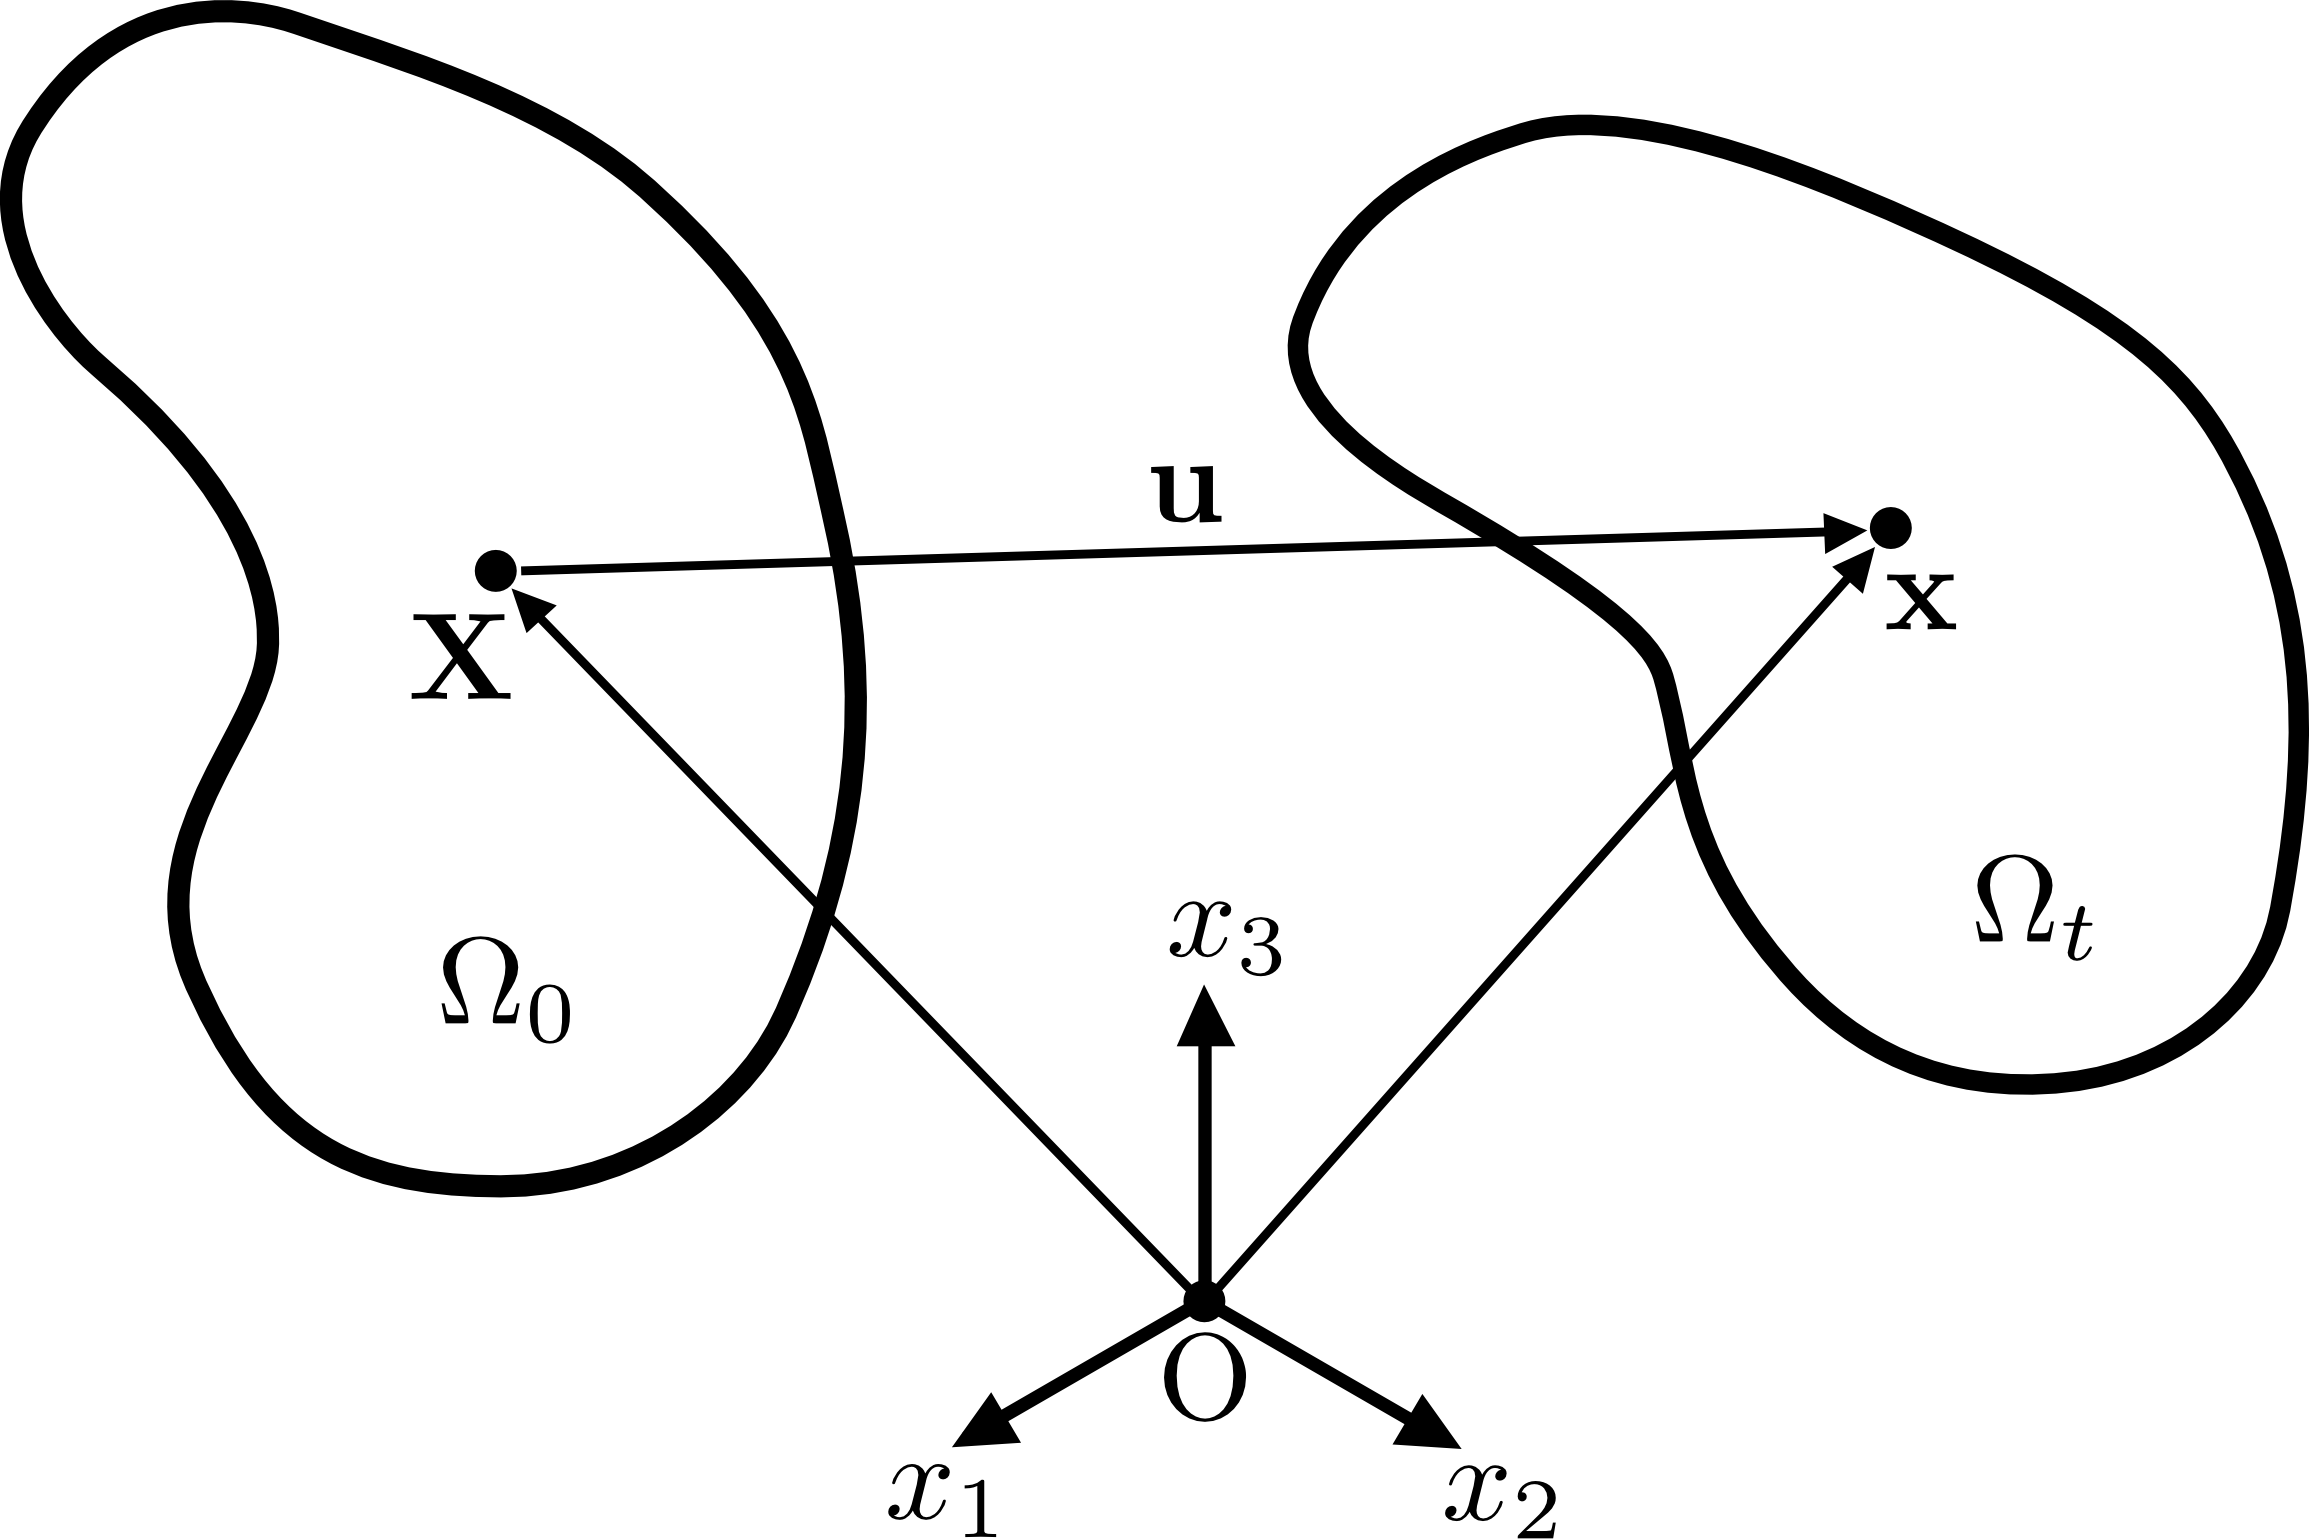
\includegraphics[width=0.6\textwidth]{figures/kinematics.png}
  \caption{A depiction of the motion of material points in a body $\Omega$.}
  \label{fig:kinematics}
\end{figure}

At a given time $t$, the Jacobian of the deformation mapping $\raisebox{\depth}{$\chi$}_t$ yields the deformation gradient $\mathbf{F} = \nabla_X \mathbf{x}$ (a rank-2 tensor), defined as
\begin{equation}
  \mathbf{F} = \frac{\partial \mathbf{x}}{\partial \mathbf{X}} = \mathbf{1} + \nabla_X \mathbf{u},
\end{equation}
where $\nabla_X$ denotes the gradient with respect to $\mathbf{X}$. The deformation gradient may be used to map differential line segments $d \mathbf{X}$, surface areas $d \mathbf{A}$, and volumes $d V$ defined in the reference configuration into their corresponding transformed quantities ($d \mathbf{x}$, $d \mathbf{a}$, $dv$) at time $t$:
\begin{equation}
  d \mathbf{x} = \mathbf{F} d \mathbf{X}
\end{equation}
\begin{equation}
  d \mathbf{a} = J \mathbf{F}^{-T} d \mathbf{A}
\end{equation}
\begin{equation}
  d v = J d V
\end{equation}
where $J \equiv \det{\mathbf{F}}$.

In a similar fashion, the spatial velocity gradient $\mathbf{L} = \nabla_x \mathbf{v}$ (where $\nabla_x$ denotes the gradient with respect to $\mathbf{x}$) may be expressed as
\begin{equation}
  \mathbf{L} = \frac{\partial \mathbf{v}}{\partial \mathbf{x}} = \frac{\partial \dot{\mathbf{x}}}{\partial \mathbf{X}} \frac{\partial \mathbf{X}}{\partial \mathbf{x}} = \dot{\mathbf{F}} \mathbf{F}^{-1},
\end{equation}
which may be further decomposed into a symmetric part $\mathbf{D}$ (the rate of deformation tensor) and an anti-symmetric part $\mathbf{W}$ (the spin tensor):
\begin{equation}
  \mathbf{D} = \frac{1}{2} (\mathbf{L} + \mathbf{L}^T), \quad \mathbf{W} = \frac{1}{2} (\mathbf{L} - \mathbf{L}^T).
\end{equation}

\subsection{Compatibility}

In continuum mechanics, compatibility refers to the idea that a given body remains a contiguous medium following some deformation described by $\raisebox{\depth}{$\chi$}_t$. In other words, $\raisebox{\depth}{$\chi$}_t$ must characterize a continuous mapping of material points between different configurations in time, such that the topology of body remains unchanged. Compatibilitiy is characterized by the following necessary and sufficient conditions:
\begin{equation}
  \nabla_X \times \mathbf{F} = \mathbf{0}.
\end{equation}
Satisfaction of the above compatibility condition implies that there exists a continuous, single-valued displacement field which gives rise to the deformation characterized by $\mathbf{F}$.

\subsection{Finite Strain Measures}

Consider the set of all material line segments $d \mathbf{X}$ which lie in a small neighborhood around a given material point $\mathbf{X}$. Also, consider these same material line segments $d \mathbf{x}$ in the current configuration of the body after some deformation corresponding to $\mathbf{F} (\mathbf{X}, t)$ has taken place, such that $d \mathbf{x} = \mathbf{F} d \mathbf{X}$.

At a given material point $\mathbf{X}$, the deformation gradient $\mathbf{F} (\mathbf{X}, t)$ may be characterized as a linear operator, which may be decomposed into two step-wise operations: a stretching operation $\mathbf{U}$ (or $\mathbf{V}$), and a rotation $\mathbf{R}$, yielding the polar decomposition of $\mathbf{F}$:
\begin{equation}
  \mathbf{F} = \mathbf{R} \mathbf{U} = \mathbf{V} \mathbf{R},
\end{equation}
where $\mathbf{U}$ is termed the right stretch tensor, and $\mathbf{V}$ is the left stretch tensor. There arise from $\mathbf{U}$ and $\mathbf{V}$ two primary deformation measures: the right Cauchy-Green deformation tensor $\mathbf{C} = \mathbf{U}^2$, and the left Cauchy-Green deformation tensor $\mathbf{B} = \mathbf{V}^2$. Each of these, in turn, yield two of the most commonly utilized finite strain measures: the Green-Lagrangian strain tensor $\mathbf{E} = \frac{1}{2} (\mathbf{C} - \mathbf{I})$, and the Eulerian-Almansi strain tensor $\mathbf{e} = \frac{1}{2} (\mathbf{I} - \mathbf{B}^{-1})$. It is not difficult to show that both of these strain measures reduce to the small strain tensor $\boldsymbol{\varepsilon} = \frac{1}{2} (\nabla_X \mathbf{u} + (\nabla_X \mathbf{u})^T)$ if the displacements are sufficiently small.

Another finite strain measure that has gained attention in more recent years is the Hencky (logarithmic, or ``true'') strain tensor $\mathbf{H} = \frac{1}{2} \log \mathbf{B}$. Because the Hencky strain tensor belongs to the Seth-Hill family of strain measures (as do the Green-Lagrangian and Eulerian-Almansi strain tensors), it likewise is seen to reduce to the small strain tensor in the limit of small displacements.

\section{Conservation of Linear and Angular Momentum}

For a given material body $\mathcal{B}_t \subset \mathbb{R}^d$, any open subset $\Omega_t \subset \mathcal{B}_t$ must satisfy Newton's second law of motion, such that the net external force which acts upon $\Omega_t$ is equal to the total change in linear momentum of the system, i.e.
\begin{equation}
  \frac{d}{dt} \int_{\Omega_t} \rho \mathbf{v} \, dv = \int_{\Omega_t} \rho \mathbf{b} \, dv + \int_{\partial \Omega_t} \mathbf{t} \, da \quad \forall \Omega_t \subset \mathcal{B},
\end{equation}
where $\rho$ is the mass density of the matertial, $\mathbf{v}$ is the velocity field, $\mathbf{b}$ is an applied body force per unit of mass, and $\mathbf{t}$ is the traction vector -- a force per unit of area -- which acts on $\partial \Omega_t$ (the boundary of $\Omega_t$). Via the Cauchy tetrahedron argument, it is possible to express the traction vector $\mathbf{t} (\mathbf{n})$ as a linear function of the unit vector $\mathbf{n}$, which is normal to the surface upon which the traction acts:
\begin{equation}
  \mathbf{t} = \mathbf{n} \cdot \boldsymbol{\sigma},
\end{equation}
where $\boldsymbol{\sigma}$ is referred to as the Cauchy stress tensor. Invoking the divergence theorem, we may utilize the above relation to convert the traction boundary integral into a volume integral over $\Omega_t$:
\begin{equation}
  \int_{\partial \Omega_t} \mathbf{t} \, da = \int_{\partial \Omega_t} \mathbf{n} \cdot \boldsymbol{\sigma} \, da = \int_{\Omega_t} \nabla_x \cdot \boldsymbol{\sigma} \, dv.
\end{equation}
Moreover, utilizing Reynolds' transport theorem, conservation of mass, and a change of variables in $\mathbf{x}$ and $\mathbf{X}$, it is possible to show that
\begin{equation}
  \frac{d}{dt} \int_{\Omega_t} \rho \mathbf{v} \, dv = \int_{\Omega_t} \rho \frac{d \mathbf{v}}{dt} \, dv,
\end{equation}
which ultimately yields
\begin{equation}
  \int_{\Omega_t} \left[ \rho (\mathbf{b} - \dot{\mathbf{v}}) + \nabla_x \cdot \boldsymbol{\sigma} \right] \, dv = \mathbf{0} \quad \forall \Omega_t \subset \mathcal{B}.
\end{equation}
Since we have imposed no limitations on the choice of subset $\Omega_t$, we may invoke the localization theorem to determine a point-wise statement of equilibrium in the body $\mathcal{B}_t$:
\begin{equation}
  \rho (\mathbf{b} - \dot{\mathbf{v}}) + \nabla_x \cdot \boldsymbol{\sigma} = \mathbf{0} \quad \forall \mathbf{x} \in \mathcal{B}_t.
\end{equation}

Similarly, by formulating an expression for the conservation of angular momentum and following an analogous procedure, we obtain an additional point-wise requirement on the symmetry of the Cauchy stress tensor:
\begin{equation}
  \boldsymbol{\sigma} = \boldsymbol{\sigma}^T \quad \forall \mathbf{x} \in \mathcal{B}_t.
\end{equation}

\subsection{Measures of Stress}

As expressed earlier, the Cauchy stress tensor $\boldsymbol{\sigma}$ relates the normal $\mathbf{n}$ of a given surface area element $d \mathbf{a} = \mathbf{n} \, da$ to the corresponding force per unit of area $\mathbf{t}$ which acts on that surface, where the surface element $d \mathbf{a}$ is defined in the current configuration of the body (at some time $t > 0$). The total force which acts on a given surface $d \mathbf{a}$ is then
\begin{equation}
  d \mathbf{f} = \mathbf{t} \, da = \boldsymbol{\sigma}^T \, d \mathbf{a}.
\end{equation}
Utilizing Nanson's formula for area transformations:
\begin{equation}
  d \mathbf{a} = J \mathbf{F}^{-T} \, d \mathbf{A},
\end{equation}
we may consider an equivalent representation of $d \mathbf{f}$, such that
\begin{equation}
  d \mathbf{f} = J \boldsymbol{\sigma}^T \mathbf{F}^{-T} \, d \mathbf{A} = \mathbf{P} \, d \mathbf{A} = \mathbf{p} \, dA,
\end{equation}
where $\mathbf{P}$ is defined as the first Piola-Kirchhoff stress tensor (which in general is not symmetric.), and where $\mathbf{p} = \mathbf{N} \cdot \mathbf{P}^T$ is the corresponding Piola traction vector, characterizing the distributed force which acts over a surface defined in the reference configuration with area $dA$ and normal $\mathbf{N}$.

Another stress measure (related to the first Piola-Kirchhoff stress) is the second Piola-Kirchhoff stress tensor $\mathbf{S}$, which is commonly defined as the pull-back of the Kirchhoff stress tensor $\boldsymbol{\tau} = J \boldsymbol{\sigma}$:
\begin{equation}
  \mathbf{S} = \mathbf{F}^{-1} \boldsymbol{\tau} \mathbf{F}^{-T}.
\end{equation}

\section{Constitutive Relations}

Fundamentally, we require there to be some relationship between the forces applied to a given body, and the observed deformation of those bodies. Such relationships are generally referred to as constitutive models, which characterize a macroscopic connection between stress and strain in a continuum.

\subsection{Models of Elasticity}

 Constitutive models have variable forms, mostly notably as they relate to notions of elasticity: the tendency of a material to revert to its original undeformed configuration if the applied forces are removed. Models for elastic material behavior fall into three primary categories: hyperelasticity, Cauchy-elasticity, and hypoelasticity.

Hyperelasticity is concerned with the description of a material's state through an elastic potential function, which characterizes the total stored elastic strain energy $W (\mathbf{F})$ in the material as a function of the total deformation measured from some (nominally undeformed) reference configuration. Differentiation of this potential with respect to a given deformation measure will yield an expression for the corresponding work-conjugate measure of stress, e.g.
\begin{equation}
  \mathbf{P} = \frac{\partial W}{\partial \mathbf{F}}, \qquad \mathbf{S} = \frac{\partial W}{\partial \mathbf{E}}.
\end{equation}
Some common examples of hyperelastic models include the St. Venant-Kirchhoff material model:
\begin{equation}
  W (\mathbf{E}) = \frac{\lambda}{2} \text{tr} (\mathbf{E})^2 + \mu \text{tr} (\mathbf{E}^2),
\end{equation}
Hencky's elasticity model:
\begin{equation}
  W (\mathbf{H}) = \frac{\lambda}{2} \text{tr} (\mathbf{H})^2 + \mu \text{tr} (\mathbf{H}^2),
\end{equation}
the compressible Mooney-Rivlin solid:
\begin{equation}
  W (I_1, I_2, J) = C_{01} (J^{-4/3} I_2 - 3) + C_{10} (J^{-2/3} I_1 - 3) + D_1 (J - 1)^2,
\end{equation}
\begin{equation}
  I_1 = \text{tr} (\mathbf{B}), \qquad I_2 = \frac{1}{2} \left[ \text{tr} (\mathbf{B})^2 - \text{tr} (\mathbf{B}^2) \right], \qquad J = \det (\mathbf{F}),
\end{equation}
\begin{equation}
  D_1 = \frac{\kappa}{2}, \qquad (C_{01} + C_{10}) = \frac{\mu}{2},
\end{equation}
and the compressible Neo-Hookean solid (a special case of the Mooney-Rivlin solid where $C_{01} = 0$, and $C_1 = C_{10}$):
\begin{equation}
  W (I_1, J) = C_1 (J^{-2/3} I_1 - 3) + D_1 (J - 1)^2
\end{equation}

Cauchy-elasticity (as a terminology to describe a particular sub-class of material models) differs from hyperelasticity in the sense that the relations between particular stress and strain measures are defined directly, and do not necessarily arise from an elastic potential function. The models of linear elasticity, in particular, are generalizations of Hooke's law, namely:
\begin{equation}
  \boldsymbol{\sigma} = \mathbf{C} \colon \boldsymbol{\varepsilon},
\end{equation}
and are suitable for small deformations, but are typically not applicable in the context of finite deformations. By comparison, Cauchy-elastic models are defined in terms of the deformation gradient $\mathbf{F}$, i.e.
\begin{equation}
  \boldsymbol{\sigma} = f (\mathbf{F}),
\end{equation}
and are more suitable in the realm of finite deformations. For such models to be considered objective under a superposed rigid rotation corresponding to $\mathbf{R}$, they must satisfy the following condition:
\begin{equation}
  \mathbf{R} \boldsymbol{\sigma} \mathbf{R}^T = f (\mathbf{R} \mathbf{F}).
\end{equation}
Nonetheless, such models may still suffer from being non-conservative, in the sense that the total work done by the stresses in moving through an arbitrary closed cycle of deformation does not necessarily sum to zero. For these reasons, models of hyperelasticity are generally preferred where the use of such models is deemed appropriate. Nonetheless elasticity models are still useful, particularly in the context of small deformations.

In contrast, hypoelasticity models define an evolution (rate) equation in terms of the current stress and the velocity gradient at a given material point, i.e.
\begin{equation}
  \dot{\boldsymbol{\sigma}} = g(\boldsymbol{\sigma}, \mathbf{L}).
\end{equation}
Hypoelasticity models are in general non-conservative, and moreover may not necessarily return to a state of zero stress following a closed cycle of deformation. Hypoelasticity is generally less appropriate where hyperelastic or other elastic models may be used instead. The value of hypoelasticity lies in its ability to accomodate models for plastic flow and dissipation in the material, giving rise to the common models of hypoelasto-plasticity.

One of the primary challenges of working with hypoelastic models concerns the manner in which the rate of stress transforms under superposed rigid-body rotations. These considerations have led to the formulation of co-rotational (or objective) stress rates. A multitude of such rates exist, though only a few are found to be in common usage. Most notably, the Jaumann rate of stress $\accentset{\circ}{\boldsymbol{\sigma}}$ is defined as
\begin{equation}
  \accentset{\circ}{\boldsymbol{\sigma}} = g (\boldsymbol{\sigma}, \mathbf{D}) = \dot{\boldsymbol{\sigma}} + \boldsymbol{\sigma} \mathbf{W} - \mathbf{W} \boldsymbol{\sigma},
\end{equation}
where $\mathbf{D}$ and $\mathbf{W}$ specify the rate of deformation and spin at a given material point, respectively.

%\subsection{Equations of Material State}
%
%In a continuum body $\mathcal{B}_t$, every material point $\mathbf{x} \in \mathcal{B}_t$ is endowed with a ``material state'' $S_t (\mathbf{x})$ at time $t$. In the context of Lagrangian solid mechanics, the material state $S_t = \left\{ \boldsymbol{\sigma}, \, q_{*} \right\}$ typically consists of the Cauchy stress tensor $\boldsymbol{\sigma}$, and any (possibly tensorial) internal state variables $q_{*}$ associated with the material model.
%
%In a computational setting, the analysis is usually subdivided into discrete time steps $\left\{ t_k \right\}_{k=0}^N$, and the motion of material points from time $t_k$ to $t_{k+1}$ is described by an incremental displacement field, denoted $\hat{\mathbf{u}} = \mathbf{u}_{k+1} - \mathbf{u}_{k}$. The deformation associated with this motion may be characterized by an incremental deformation gradient $\hat{\mathbf{F}} = \partial \mathbf{x}_{k+1} / \partial \mathbf{x}_k = \mathbf{1} + \nabla_{x_k} \hat{\mathbf{u}}$.
%
%Assuming that the material behaves in a rate-independent manner, a generic constitutive model $f \colon (S_k, \nabla_{x_k} \hat{\mathbf{u}}) \mapsto S_{k+1}$ should yield the updated material state $S_{k+1}$ at time $t_{k+1}$ as a function of the material state $S_k$ at time $t_k$, and the incremental displacement gradient $\nabla_{x_k} \hat{\mathbf{u}}$.

\section{Model Boundary Value Problem}

Up to this point, we have discussed only the essential relationships which exist between physical quantities of interest in the context of solid mechanics. Ultimately, however, we should like to determine the anticipated motion and deformation of a particular body under the action of pre-determined externally applied forces. To this end, we must turn our attention to the definition -- and solution -- of a corresponding boundary value problem (BVP). Such problems must be well-posed, in the sense that there exists a unique solution to the stated problem, thereby imposing certain restrictions on the choice of boundary conditions.

\subsection{The Strong Form Statement of Equilibrium}

In the context of solid mechanics, the solution of a given boundary value problem usually refers to a complete description of the primary field variable(s) of interest, namely the displacement field $\mathbf{u} (\mathbf{X})$ at all locations $\mathbf{X} \in \mathcal{B}_0$ within the body $\mathcal{B}_0$ in its reference configuration. Under the requirements of compatibility, we presume that the displacement field is a continuous function, whose derivatives up to second order are defined everywhere, i.e. $\mathbf{u} \in \left[ C^2 (\mathcal{B}_0) \right]^d$.

Now, let us examine a quasi-static solid mechanics model problem of the following form: consider an open domain $\mathcal{B}_0 \subset \mathbb{R}^d$ whose boundary $\partial \mathcal{B}_0$ consists of the partition $\left\{ \Gamma_u, \Gamma_t \right\}$. Let $\mathbf{u} = \bar{\mathbf{u}} \, \, \forall \mathbf{X} \in \Gamma_u$ constitute a prescribed Dirichlet boundary condition imposed upon the displacement field, and $\mathbf{n} \cdot \boldsymbol{\sigma} = \bar{\mathbf{t}} \, \, \forall \mathbf{X} \in \Gamma_t$ be a Neumann boundary condition imposed upon the surface traction. Additionally, let us suppose that an applied body force $\mathbf{b}$ acts upon all points $\mathbf{X} \in \mathcal{B}_0$. Given these conditions, we should like to determine the displacement field $\mathbf{u} \in \mathcal{S} = \left\{ \mathbf{u} \in \left[ C^2 (\mathcal{B}_0) \right]^d \colon \mathbf{u} = \bar{\mathbf{u}} \, \, \forall \mathbf{x} \in \Gamma_u \right\}$ which satisfies the equations of equilibrium in a point-wise sense:
\begin{equation}
  \rho \mathbf{b} + \nabla_x \cdot \boldsymbol{\sigma} = \mathbf{0} \quad \forall \mathbf{x} \in \mathcal{B}_t,
\end{equation}
and where we suppose that a constitutive model has been defined in order to relate some measure of the deformation (e.g. $\mathbf{F} = \mathbf{1} + \nabla_X \mathbf{u}$) to the stress (e.g. $\boldsymbol{\sigma} = f (\mathbf{F})$). Equivalently, we may write the equations of equilibrium in terms of quantities related to the reference configuration of the body:
\begin{equation}
  \rho_0 \mathbf{b} + \nabla_X \cdot \mathbf{P}^T = \mathbf{0} \quad \forall \mathbf{X} \in \mathcal{B}_0,
\end{equation}
where $\rho_0 = J \rho$ is the mass density of the material at time $t = 0$. The above statement is commonly referred to as the ``strong form'' of the model problem, given that it requires a point-wise satisfaction of equilibrium.

It should be emphasized that the Dirichlet boundary conditions and the requirements of compatibility are satisfied implicitly, as a consequence of the deliberate choice of function space $\mathcal{S}$ for the displacement field. Such functions $\mathbf{u} \in \mathcal{S}$ are termed ``admissible,'' as potential solutions to the boundary value problem at hand.

\subsection{The Equivalent Weak Form Statement of Equilibrium}

In general, solutions to the strong form problem are not easily obtained. For this reason, it proves to be much more convenient to work with the (equivalent) ``weak form'' statement of the boundary value problem:

\textit{Find $\mathbf{u} \in \mathcal{S} = \left\{ \mathbf{u} \in \left[H^{1} (\mathcal{B}_0)\right]^d \colon \mathbf{u} = \bar{\mathbf{u}} \, \, \forall \mathbf{X} \in \Gamma_u \right\}$ such that}
\begin{equation}
  \int_{\raisebox{\depth}{$\chi$} (\mathcal{B}_0, t)} \rho \mathbf{b} \cdot \mathbf{v} \, dv + \int_{\raisebox{\depth}{$\chi$} (\Gamma_t, t)} \bar{\mathbf{t}} \cdot \mathbf{v} \, da - \int_{\raisebox{\depth}{$\chi$} (\mathcal{B}_0, t)} \boldsymbol{\sigma} \colon \nabla_x \mathbf{v} \, dv = 0 \quad \forall \mathbf{v} \in \mathcal{V},
  \label{eq:weakeulerian}
\end{equation}
\textit{or equivalently}
\begin{equation}
  \int_{\mathcal{B}_0} \rho_0 \mathbf{b} \cdot \mathbf{v} \, dV + \int_{\Gamma_t} \bar{\mathbf{p}} \cdot \mathbf{v} \, dA - \int_{\mathcal{B}_0} \mathbf{P} \colon \nabla_X \mathbf{v} \, dV = 0 \quad \forall \mathbf{v} \in \mathcal{V},
  \label{eq:weaklagrangian}
\end{equation}
\textit{where $\mathcal{V} = \left\{ \mathbf{v} \in \left[H^{1} (\mathcal{B}_0)\right]^d \colon \mathbf{v} = \mathbf{0} \, \, \forall \mathbf{X} \in \Gamma_u \right\}$, and}
\begin{equation}
  H^{1} (\mathcal{B}_0) = \left\{ u \in L^2 (\mathcal{B}_0), \, D^{\alpha} u \in L^2 (\mathcal{B}_0) \, \, \forall | \alpha | \leq 1 \right\}.
\end{equation}
In (\ref{eq:weaklagrangian}), the traction boundary condition has been replaced by $\mathbf{p} = \bar{\mathbf{p}} \, \, \forall \mathbf{X} \in \Gamma_t$ -- i.e. a condition on the Piola (rather than Cauchy) surface traction. The function space $\mathcal{S}$ is commonly referred to as the space of admissible ``trial solutions,'' whereas $\mathcal{V}$ is called the space of ``test functions,'' and consists of all admissible variations such that $\mathcal{V} = T_{\mathbf{u}} \mathcal{S}$ is the tangent space to $\mathcal{S}$ (i.e. $\mathbf{u} + \mathbf{v} \in \mathcal{S} \, \, \forall \mathbf{u} \in \mathcal{S}, \, \mathbf{v} \in \mathcal{V}$). In words, our goal is determine the solution $\mathbf{u}$ from among all admissible trial solutions contained in $\mathcal{S}$ which satisfies equation (\ref{eq:weakeulerian}) or (\ref{eq:weaklagrangian}) for all admissible variations $\mathbf{v} \in \mathcal{V}$.

Under the assumptions of small displacements and linear elasticity, equations (\ref{eq:weakeulerian}) and (\ref{eq:weaklagrangian}) are equivalent, and may be more succinctly expressed in terms of a bilinear form $a(\cdot, \cdot) \colon \mathcal{S} \times \mathcal{V} \mapsto \mathbb{R}$ and a linear form $\ell (\cdot) : \mathcal{V} \mapsto \mathbb{R}$ such that
\begin{equation}
  a(\mathbf{u}, \mathbf{v}) + \ell (\mathbf{v}) = 0 \quad \forall \mathbf{v} \in \mathcal{V}.
\end{equation}


\section{Galerkin Approximations to the Weak Form}

In the weak form problem statement, the trial and test spaces $\mathcal{S}$ and $\mathcal{V}$ are taken to be infinite dimensional function spaces. In a practical computational setting, however, this renders the solution of such problems infeasible. Instead, most variational methods consider approximate solutions to the weak form, where $\mathbf{u} \in \mathcal{S}$ and $\mathbf{v} \in \mathcal{V}$ are replaced by $\mathbf{u}^h \in \mathcal{S}^h \subset \mathcal{S}$ and $\mathbf{v}^h \in \mathcal{V}^h \subset \mathcal{V}$, respectively. In this context, $\mathcal{S}^h = \left\{ \varphi_a \right\}_{a = 1}^{N}$ and $\mathcal{V}^h = \left\{ \phi_a \right\}_{a = 1}^{M}$ denote finite dimensional sub-spaces of $\mathcal{S}$ and $\mathcal{V}$, such that
\begin{equation}
  \mathbf{u}^h = \sum_{a = 1}^N \varphi_a \mathbf{u}_a, \qquad \mathbf{v}^h = \sum_{a = 1}^M \phi_a \mathbf{v}_a.
\end{equation}

This yields the Galerkin approximation to the weak form:
\textit{Find $\mathbf{u}^h \in \mathcal{S}^h$ such that}
\begin{equation}
  \int_{\mathcal{B}_t} \rho \mathbf{b} \cdot \mathbf{v}^h \, dv + \int_{\raisebox{\depth}{$\chi$} (\Gamma_t, t)} \bar{\mathbf{t}} \cdot \mathbf{v}^h \, da - \int_{\mathcal{B}_t} \boldsymbol{\sigma} \colon \nabla_x \mathbf{v}^h \, dv = 0 \quad \forall \mathbf{v}^h \in \mathcal{V}^h,
  \label{eq:approxweakeulerian}
\end{equation}
\textit{or equivalently}
\begin{equation}
  \int_{\mathcal{B}_0} \rho_0 \mathbf{b} \cdot \mathbf{v}^h \, dV + \int_{\Gamma_t} \bar{\mathbf{p}} \cdot \mathbf{v}^h \, dA - \int_{\mathcal{B}_0} \mathbf{P} \colon \nabla_X \mathbf{v}^h \, dV = 0 \quad \forall \mathbf{v}^h \in \mathcal{V}^h.
  \label{eq:approxweaklagrangian}
\end{equation}

Without loss of generality, if we suppose that $\mathcal{S} = \mathcal{V}$ (provided $\mathbf{u} = \mathbf{0} \, \, \forall \mathbf{X} \in \Gamma_u$), then we may select identical sub-spaces $\mathcal{S}^h = \mathcal{V}^h = \left\{ \varphi_a \right\}_{a = 1}^{N}$, resulting in a symmetric (or Bubnov-) Galerkin method. Traditional finite element methods fall into this category. Such methods are advantageous in the sense that (for linear problems) they result in stable, symmetric bilinear forms satisfying the Galerkin orthgonality (or ``best approximation'') property -- the property that the solution error $\mathbf{e} = \mathbf{u}^h - \mathbf{u}$ is orthogonal to the chosen sub-space $\mathcal{S}^h$. This is a direct consequence of $\mathcal{V}^h = T_{\mathbf{u}^h} \mathcal{S}^h$ (i.e. $\mathbf{u}^h + \mathbf{v}^h \in \mathcal{S}^h \, \, \forall \mathbf{u}^h \in \mathcal{S}^h, \, \mathbf{v}^h \in \mathcal{V}^h$).

Petrov-Galerkin methods consider the more general case where $\mathcal{V}^h \neq \mathcal{S}^h$, resulting in differing trial and test function spaces. Such methods must guarantee satisfaction of the LBB (inf-sup) conditions to achieve convergence. Consequently, the selection of appropriate trial and test function spaces which result in stable discretizations is not trivial. Nonetheless, Petrov-Galerkin methods allow for greater flexibility in the construction of numerical approximation schemes.

\subsection{Finite Element Methods}

Finite element methods (FEM) are predicated on the idea that a problem domain $\mathcal{B}$ can be discretized into a finite number of simpler sub-domains $\omega_e \subset \mathcal{B}$, individually called elements, and collectively referred to as a ``mesh.'' The basis functions are assumed to be low-order polynomials within each element, and are compactly supported over a given patch of elements. The traditional finite element method assumes these basis functions to be $C^0$ continuous at element boundaries, yielding a priori satisfaction of compatibility.

Individual FE basis functions $\varphi_a$ are typically associated with the ``nodes'' $\mathbf{X}_a$ of the mesh (located at element verticies, along element edges, etc.), such that the kronecker delta property is satisfied:
\begin{equation}
	\mathbf{u}^h (\mathbf{X}_b) = \sum_{a = 1}^N \varphi_a (\mathbf{X}_b) \mathbf{u}_a = \mathbf{u}_b.
\end{equation}
Consequently, the basis functions comprise a set of interpolants for discrete values of the solution defined at the nodes.

Elements consisting of regular shapes (tetrahedra, hexahedra) also provide a natural means of effecting numerical integration of the weak form through the use of the isoparametric transformation and product Gaussian quadrature rules.

\section{Requirements for Convergence of an \\ Approximation Method}

Because variational methods utilize finite dimensional approximations $\mathbf{u}^h \in \mathcal{S}^h$ and $\mathbf{v}^h \in \mathcal{V}^h$, they inherrently incur some error $\mathbf{e} = \mathbf{u}^h - \mathbf{u}$ in approximating the exact solution to the original boundary value problem. The  approximation power of a given method is typically characterized by the rate at which a specified error measure $||\mathbf{e}||$ becomes smaller as the dimension of the approximation spaces $\mathcal{S}^h$ and $\mathcal{V}^h$ are systematically increased.

\subsection{Satisfaction of Essential Boundary Conditions}



\subsection{Completeness/Approximability}



\subsection{Variational Consistency}



\subsubsection{Constraints on Numerical Quadrature}



\subsection{Numerical Stability}
\subsubsection{The Inf-Sup Condition}
\subsection{Tests for Convergence}
\subsubsection{The Irons Patch Test}
\subsubsection{The Generalized Patch Test}
\subsubsection{The F-E-M Test}

\section{Nonlinear Solution Methods}
\subsection{Finite Deformations and Nonlinear Kinematics}
\subsection{Nonlinear Material Behavior}
\subsection{Requirements of the Approximation Method}

%\documentclass[12pt]{book}

\usepackage[us,nodayofweek,12hr]{datetime}
\usepackage{graphicx}
%\usepackage[square,comma,numbers,sort&compress]{natbib}
%\usepackage{hypernat}
% Other useful packages to try
\usepackage{amsmath}
\usepackage{amssymb}
\usepackage{accents}
\usepackage[]{algorithm2e}
\usepackage{caption}
\usepackage{subcaption}

\begin{document}

\chapter{Sources of Solution Inaccuracy in Computational Solid Mechanics}
%
\section{Manifestations of Finite Element Locking Phenomena}

\subsection{Volumetric Locking}

\subsection{Shear Locking}

\subsection{Element Distortion Sensitivity}

\section{A Mathematical Treatment of Locking}

\section{Mitigation Techniques}

(A review of various approaches that have been taken to solve the aforementioned problem, and an assessment of their relative efficacies (advantages, disadvantages), possibly presented in chronological order, though it may be acceptable to present the material in a format that organizes different methodologies according to the degree of similarity in their approach. The variety of different approaches should be justified based on their intended applications, and should additionally illustrate the fact that the issue being addressed is one which has yet to be fully solved in a robust and general way. Include most of the references within this section and its relevant sub-sections. All references should be made relevant to the subject, and not meandering.)

\subsection{Higher-order Discretizations}
\subsubsection{Selective $p$-Refinement}

\subsection{Strain Projection Methods}
\subsubsection{Selective Reduced Integration}
\subsubsection{The B-Bar Method for Linear Problems}

Consider a displacement interpolant on an element with $N$ nodes:
\begin{equation}
  u_i (\mathbf{x}) = \sum_{a = 1}^N \varphi_a (\mathbf{x}) u_{ai},
\end{equation}
\begin{equation}
  u_{i,j} (\mathbf{x}) = \sum_{a = 1}^N \varphi_{a,j} (\mathbf{x}) u_{ai}.
\end{equation}
In the context of small deformations, we may write the linearized strain tensor $\boldsymbol{\varepsilon}$ as
\begin{equation}
  \varepsilon_{ij} (\mathbf{x}) = \frac{1}{2} (u_{i,j} + u_{j,i}) = \sum_{a = 1}^N \frac{1}{2} (\varphi_{a,j} \delta_{ik} + \varphi_{a,i} \delta_{jk}) u_{ak} = \sum_{a = 1}^N B_{ijak} u_{ak},
\end{equation}
and the trace -- or dilatation, $\epsilon$ -- of the small strain tensor as
\begin{equation}
  \epsilon (\mathbf{x}) = \frac{1}{3} \varepsilon_{ii} = \sum_{a = 1}^N \frac{1}{3} (\varphi_{a,i} \delta_{ik}) u_{ak} = \sum_{a = 1}^N B^\epsilon_{ak} u_{ak}.
\end{equation}
The deviatoric part of the strain $\mathbf{e}$ is then
\begin{equation}
  e_{ij} = \varepsilon_{ij} - \epsilon \delta_{ij} = \sum_{a = 1}^N \frac{1}{6} \left[ 3(\varphi_{a,j} \delta_{ik} + \varphi_{a,i} \delta_{jk}) - 2 \delta_{ij} (\varphi_{a,l} \delta_{lk}) \right] u_{ak} = \sum_{a = 1}^N B^e_{ijak} u_{ak},
\end{equation}
and we may consider an additive decomposition of the strain into volumetric and deviatoric parts:
\begin{equation}
  \varepsilon_{ij} = e_{ij} + \epsilon \delta_{ij} = \sum_{a = 1}^N \left[ B^e_{ijak} + B^\epsilon_{ak} \delta_{ij} \right] u_{ak}.
\end{equation}

The B-bar approach essentially considers a projection of the volumetric strain operator $B^\epsilon_{ak} (\mathbf{x})$ onto a carefully selected sub-space $S$ of functions defined over the element. In general, this sub-space is spanned by an orthonormal basis $\left\{ \xi_k \right\}_{k = 1}^{M}$ with respect to the norm induced by the $L^2 (\Omega_e)$ inner-product, i.e.
\begin{equation}
  || \xi_k ||_{\Omega_e} = \sqrt{\langle \xi_k, \xi_k \rangle_{\Omega_e}} = \left[ \int_{\Omega_e} \xi_k \cdot \xi_k \, d \Omega \right]^{1/2} = 1 \quad \forall k,
\end{equation}
and $\langle \xi_k, \xi_l \rangle_{\Omega_e} = 0 \, \forall k \neq l$. The $L^2$ projection of an arbitrary field $\epsilon (\mathbf{x})$ onto the chosen sub-space $S$ is obtained via
\begin{equation}
  \bar{\epsilon} (\mathbf{x}) = \sum_{k=1}^{M} \langle \epsilon, \xi_k \rangle_{\Omega_e} \xi_k (\mathbf{x}),
\end{equation}
and if numerical quadrature is utilized, then
\begin{equation}
  \langle f, g \rangle_{\Omega_e} \approx \langle f, g \rangle^q_{\Omega_e} = \sum_{q=1}^{P} w_q f (\mathbf{x}_q) \cdot g (\mathbf{x}_q),
\end{equation}
\begin{equation}
  \bar{\epsilon} (\mathbf{x}) = \sum_{k=1}^{M} \langle \epsilon, \xi_k \rangle^q_{\Omega_e} \xi_k (\mathbf{x}).
\end{equation}
Consequently, we may consider a projection of the operator $B^\epsilon_{ak} (\mathbf{x})$ onto $S$, resulting in
\begin{equation}
  \bar{B}^\epsilon_{ak} (\mathbf{x}) = \sum_{k=1}^{M} \langle B^\epsilon_{ak}, \xi_k \rangle^q_{\Omega_e} \xi_k (\mathbf{x}),
\end{equation}
which is ultimately used in the final B-bar expression for the projected strain $\tilde{\boldsymbol{\varepsilon}}$:
\begin{equation}
  \tilde{\varepsilon}_{ij} (\mathbf{x}) = e_{ij} + \bar{\epsilon} \delta_{ij} = \sum_{a = 1}^N \left[ B^e_{ijak} + \bar{B}^\epsilon_{ak} \delta_{ij} \right] u_{ak} = \sum_{a = 1}^N \tilde{B}_{ijak} u_{ak}.
\end{equation}

The modified strain-displacement operator $\tilde{B}_{ijak}$ may be computed and stored ahead of time, if so desired. Moreover, if we now suppose that the strain field has been replaced by $\tilde{\boldsymbol{\varepsilon}} = \frac{1}{2} (\tilde{\nabla} \mathbf{u} + (\tilde{\nabla} \mathbf{u})^T)$ which arises from a modified gradient operator $\tilde{\nabla}$, then we may additionally define a correspondingly modified divergence operator $\tilde{\nabla} \cdot$, such that the resulting (symmetric) element stiffness matrix $K_{aibj}$ may be written
\begin{equation}
  K_{aibj} = \int_{\Omega_e} \tilde{B}_{mnai} C_{mnpq} \tilde{B}_{pqbj} \, d \Omega,
\end{equation}
where $C_{mnpq}$ is the rank-4 modulus tensor of linear elasticity.

The question now turns to whether there exists an interpolating basis $\left\{ \varphi_a \right\}_{a=1}^N$ whose gradients $\nabla \varphi_a$ yield the modified strain-displacement operator $\tilde{B}_{ijak}$ directly. The answer is a most definitive no, as easily seen by the sparsity of $B_{ijak}$:
\begin{equation}
  \left\{ \begin{array}{c} \varepsilon_{11} \\ \varepsilon_{22} \\ \varepsilon_{33} \\ \varepsilon_{23} \\ \varepsilon_{13} \\ \varepsilon_{12} \end{array} \right\} = \sum_{a = 1}^{N} \left[ \begin{array}{ccc} B_{11a1} & 0 & 0 \\ 0 & B_{22a2} & 0 \\ 0 & 0 & B_{33a3} \\ 0 & B_{23a2} & B_{23a3} \\ B_{13a1} & 0 & B_{13a3} \\ B_{12a1} & B_{12a2} & 0 \end{array} \right] \left\{ \begin{array}{c} u_{a1} \\ u_{a2} \\ u_{a3} \end{array} \right\},
\end{equation}
as compared to $\tilde{B}_{ijak}$:
\begin{equation}
  \left\{ \begin{array}{c} \tilde{\varepsilon}_{11} \\ \tilde{\varepsilon}_{22} \\ \tilde{\varepsilon}_{33} \\ \tilde{\varepsilon}_{23} \\ \tilde{\varepsilon}_{13} \\ \tilde{\varepsilon}_{12} \end{array} \right\} = \sum_{a = 1}^{N} \left[ \begin{array}{ccc} \tilde{B}_{11a1} & \tilde{B}_{11a2} & \tilde{B}_{11a3} \\ \tilde{B}_{22a1} & \tilde{B}_{22a2} & \tilde{B}_{22a3} \\ \tilde{B}_{33a1} & \tilde{B}_{33a2} & \tilde{B}_{33a3} \\ 0 & \tilde{B}_{23a2} & \tilde{B}_{23a3} \\ \tilde{B}_{13a1} & 0 & \tilde{B}_{13a3} \\ \tilde{B}_{12a1} & \tilde{B}_{12a2} & 0 \end{array} \right] \left\{ \begin{array}{c} u_{a1} \\ u_{a2} \\ u_{a3} \end{array} \right\}.
\end{equation}
The only way that this would be possible is if a collection of enhanced strain functions $\left\{ G_{\alpha ij} \right\}_{\alpha = 1}^A$ were introduced:
\begin{equation}
  \tilde{u}_{i,j} (\mathbf{x}) = \sum_{a = 1}^N \varphi_{a,j} (\mathbf{x}) u_{ai} + \sum_{\alpha=1}^A G_{\alpha ij} d_{\alpha},
\end{equation}
\begin{equation}
  \tilde{\varepsilon}_{ij} (\mathbf{x}) = \sum_{a = 1}^N B_{ijak} u_{ak} + \sum_{\alpha=1}^A G^s_{\alpha ij} d_{\alpha},
\end{equation}
where the unknown parameters $d_{\alpha}$ are selected to minimize the strain functional:
\begin{equation}
  \min_{d_{\alpha}} E,
\end{equation}
\begin{equation}
  E = \frac{1}{2} || \tilde{\boldsymbol{\varepsilon}} ||^2_{\Omega_e} = \frac{1}{2} \int_{\Omega_e} \tilde{\boldsymbol{\varepsilon}} \colon \tilde{\boldsymbol{\varepsilon}} \, d \Omega.
\end{equation}
Consequently,
\begin{equation}
  \frac{\partial E}{\partial d_{\beta}} = \langle \tilde{\boldsymbol{\varepsilon}}, \frac{\partial \tilde{\boldsymbol{\varepsilon}}}{\partial d_{\beta}} \rangle_{\Omega_e} = \langle \tilde{\boldsymbol{\varepsilon}}, \mathbf{G}^s_{\beta} \rangle_{\Omega_e} = 0 \quad \forall \beta,
\end{equation}
yielding the system of equations:
\begin{equation}
  \sum_{\alpha=1}^A \langle \mathbf{G}^s_{\alpha}, \mathbf{G}^s_{\beta} \rangle_{\Omega_e} d_{\alpha} = - \sum_{a = 1}^N \langle \mathbf{B}_{ak}, \mathbf{G}^s_{\beta} \rangle_{\Omega_e} u_{ak} \quad \forall \beta.
\end{equation}
If we were judicious in selecting a set of orthonormal enhancement functions such that $\langle \mathbf{G}^s_{\alpha}, \mathbf{G}^s_{\beta} \rangle_{\Omega_e} = \delta_{\alpha \beta}$, then we may express the enhanced strain field only in terms of the nodal displacements:
\begin{equation}
  \tilde{\varepsilon}_{ij} (\mathbf{x}) = \sum_{a = 1}^N \left[ B_{ijak} - \sum_{\alpha=1}^A \langle \mathbf{B}_{ak}, \mathbf{G}^s_{\alpha} \rangle_{\Omega_e} G^s_{\alpha ij} \right] u_{ak}.
\end{equation}

It is not difficult to see that this approach is identical in nature to the strain projection method presented earlier (specifically, if the enhancement functions are chosen such that $G_{\alpha ij} = \frac{1}{\sqrt{3}} \delta_{ij} \eta_{\alpha}$). In this case, the sub-space $S = \left\{ \xi_k \right\}_{k=1}^M$ onto which the strains are projected is defined through the complementary sub-space $\left\{ \eta_{\alpha} \right\}_{\alpha = 1}^A$.

\subsubsection{The F-Bar Method for Nonlinear Kinematics}

In likeness to the B-bar method for linear problems, the F-bar approach may be thought of as an extension of the method to non-linear problems involving finite deformations. Rather than strain, however, the primary quantity of interest is the deformation gradient $\mathbf{F}$, which must be appropriately modified so as to yield (in most applications) constant Jacobian $J = \det (\mathbf{F})$ throughout the element.

Proceeding along these lines, we may consider a multiplicative decomposition of the deformation gradient:
\begin{equation}
  F_{ij} (\mathbf{x}) = \delta_{ij} + u_{i,j} = \delta_{ij} + \sum_{a=1}^N \varphi_{a,j} u_{ai} = J H_{ij}
\end{equation}
where $J = \det (\mathbf{F})$, and
\begin{equation}
  H_{ij} (\mathbf{x}) = J^{-1} F_{ij}.
\end{equation}
Ultimately, we seek an expression for the enhanced deformation gradient $\tilde{\mathbf{F}}$ of the form
\begin{equation}
  \tilde{\mathbf{F}} (\mathbf{x}) = \bar{J} \mathbf{H},
\end{equation}
with $\bar{J}$ denoting the projection of the Jacobian onto a carefully selected subspace $S$ spanned by the orthonormal basis $\left\{ \xi_k \right\}_{k = 1}^M$, such that
\begin{equation}
  \bar{J} (\mathbf{x}) = \sum_{k=1}^M \langle J, \xi_k \rangle_{\Omega_e} \xi_k (\mathbf{x}).
\end{equation}
The final expression for the modified $\tilde{\mathbf{F}}$ is
\begin{equation}
  \tilde{\mathbf{F}} (\mathbf{x}) = \sum_{k=1}^M \langle J, \xi_k \rangle_{\Omega_e} \xi_k \mathbf{H}.
\end{equation}

In analog to the B-bar approach, we may also alternatively consider the inclusion of a number of enhancement functions $\left\{ G_{\alpha ij} \right\}_{\alpha = 1}^A$, such that
\begin{equation}
  \bar{F}_{ij} (\mathbf{x}) = \exp \bigg( \sum_{\alpha = 1}^A G_{\alpha ij} d_{\alpha} \bigg),
\end{equation}
which subsequently yields the enhanced deformation gradient:
\begin{equation}
  \tilde{F}_{ij} (\mathbf{x}) = \bar{F}_{ik} F_{kj}.
\end{equation}
If we constrain the enhancement functions to lie only within the sub-space of spherical tensors, i.e. $G_{\alpha ij} = \delta_{ij} \eta_{\alpha} \, \forall \alpha$, then we observe that $\mathbf{F}$ and $\bar{\mathbf{F}}$ commute, and we may write
\begin{equation}
  \bar{J} (\mathbf{x}) = \exp \bigg( 3 \sum_{\alpha = 1}^A \eta_{\alpha} d_{\alpha} \bigg),
\end{equation}
\begin{equation}
  \tilde{F}_{ij} (\mathbf{x}) = \sqrt[3]{\bar{J}} F_{ij}.
\end{equation}
Our goal now is to minimize $E$ with respect to $d_\alpha$, where
\begin{equation}
  E = \frac{1}{2} || \log \tilde{\mathbf{V}} ||^2_{\Omega_e} = \frac{1}{2} || \log \tilde{\mathbf{U}} ||^2_{\Omega_e} = \frac{1}{2} \int_{\Omega_e} \log \tilde{\mathbf{U}} \colon \log \tilde{\mathbf{U}} \, d \Omega,
\end{equation}
and
\begin{equation}
  \log \tilde{\mathbf{U}} = \frac{1}{2} \log \tilde{\mathbf{F}}^T \tilde{\mathbf{F}} = \left[ \sum_{\alpha = 1}^A \eta_{\alpha} d_{\alpha} \right] \mathbf{I} + \log \mathbf{U}.
\end{equation}
Consequently,
\begin{equation}
  \frac{\partial E}{\partial d_{\beta}} = \langle \log \tilde{\mathbf{U}}, \frac{\partial \log \tilde{\mathbf{U}}}{\partial d_{\beta}} \rangle_{\Omega_e} = \langle \log \tilde{\mathbf{U}}, \mathbf{I} \eta_{\beta} \rangle_{\Omega_e} = 0 \quad \forall \beta,
\end{equation}
yielding the system of equations:
\begin{equation}
  \sum_{\alpha=1}^A \langle \eta_{\alpha}, \eta_{\beta} \rangle_{\Omega_e} d_{\alpha} = - \langle \text{tr} (\log \mathbf{U}), \eta_{\beta} \rangle_{\Omega_e} \quad \forall \beta.
\end{equation}
Once again, if we are judicious in selecting a set of orthonormal enhancement functions such that $\langle \eta_{\alpha}, \eta_{\beta} \rangle_{\Omega_e} = \delta_{\alpha \beta}$, then we may express the enhanced deformation gradient (implicitly) in terms of the nodal displacements:
\begin{equation}
  \tilde{\mathbf{F}} (\mathbf{x}) = \exp \bigg( - \sum_{\alpha = 1}^A \langle \text{tr} (\log \mathbf{U}), \eta_{\alpha} \rangle_{\Omega_e} \eta_{\alpha} \bigg) \mathbf{F} = \sum_{\alpha = 1}^A \langle J^{-1}, e^{\eta_{\alpha}} \rangle_{\Omega_e} e^{\eta_{\alpha}} \mathbf{F}.
\end{equation}

Recall that the sub-space spanned by the enhancement functions $\left\{ \eta_{\alpha} \right\}_{\alpha = 1}^A$ is complementary to the sub-space $S = \left\{ \xi_k \right\}_{k = 1}^M$ onto which the Jacobian will ultimately be projected. In some cases, it may prove to be more convenient/effective to work in terms of the sub-space $S$. For example, if our goal is to constrain $J$ to remain constant over the element, then we should specify $S$ such that it contains a single basis function which defines a constant variation of $J$ throughout the element.

In other situations, it may be relevant to try to construct an ``optimal'' set of enhancement functions which preserve crucial variations in $J$, but which otherwise attempt to address spurious variations which contribute to locking. Such enhancements may be obtained via the construction of so-called ``bubble'' functions, satisfying certain continuity and smoothness requirements, but which are otherwise selected on the basis of minimizing some measure of the ``average'' volumetric dilatation. In words: from among all possible enhancement functions (which are not strictly orthogonal to the original approximation space), we should like to find the augmenting function which optimally minimizes the stored dilatational energy in the material, i.e.
\begin{equation}
  \min_{|| \eta ||_{\Omega_e} = 1} || \text{tr} (\log \tilde{\mathbf{U}}) ||_{\Omega_e}
\end{equation}
The key here is that the space of suitable enhancement functions must be strictly orthogonal to certain sub-spaces whose properties must be preserved, i.e. any sub-spaces in which (polynomial) completeness is necessary. Otherwise, the enhancement functions should be designed to minimize the above objective over the range of all possible $\mathbf{U}$'s, taken together with a competing objective: minimize the difference between the enhancement function and the existing space of interpolants.

Suppose that $U$ denotes the vector space of functions which span all possible variations in $\log J$ over an element $\Omega_e$. A useful relation arises in considering an alternative representation for $\log J$ when one invokes the definition of the matrix logarithm:
\begin{equation}
  \log J = \log (\det (\mathbf{F})) = \log (\det (\mathbf{U})) = \frac{1}{2} \text{tr} (\log (\mathbf{C})) = \frac{1}{2} \text{tr} (\log (\mathbf{F}^T \mathbf{F}))
\end{equation}

Given some $\mathbf{D}$ and $\mathbf{W}$, it is possible to construct a corresponding stretch $\mathbf{U} = \exp (\mathbf{D})$ and rotation $\mathbf{R} = \exp (\mathbf{W})$ which together may be composed to form $\mathbf{F} = \mathbf{R} \mathbf{U} = \exp (\mathbf{W} \mathbf{D})$

\subsection{Ad Hoc Stabilization Techniques}
\subsubsection{Hourglass Control}
\subsubsection{VEM Stabilization}

\subsection{Mixed Discretization Methods}

\subsection{The Method of Incompatible Modes}
\subsubsection{Enhanced/Assumed Strain Methods}
\end{document}
\chapter{Partitioned Element Methods} \label{ch:pem}
%
This chapter defines a general class of polytopal element formulations referred to as partitioned element methods (PEM). The essential characteristics and mathematical requirements placed upon these methods are formally stated, giving rise to a family of different approaches, for which some formal investigations are conducted in subsequent chapters. Several specific formulations are summarized in detail, and a number of existing methods are herein classified as particular instances of partitioned element methods.

\section{Overview}

	% reiterate the desire for robust, arbitrary polytopal elements
	% reiterate the shortcomings of generalized barycentric coordinates
	% reiterate the shortcomings of VEM
	% PEM considers the construction of shape functions to be a special type of local approximation problem
		% need to determine well-behaved interpolants on element domains
		% can pose this as a boundary value problem
		% approximate its solution using existing methods (FEM, etc.)
		% yields relatively simple representation of shape functions
			% i.e. piece-wise polynomial
		% may utilize the discretization to define simple quadrature rules
			% e.g. composite mid-point rules
			% can enhance accuracy of these rules using gradient correction
	% Some questions:
		% how refined must the element's local discretization be to matain a sufficient level of accuracy?
			% is a coarse discretiztion sufficient?
		% what BVP should be used?
			% Laplace's equation? (harmonic SFs)
			% specification of BVP determines quality/robustness of SFs
		% are certain approximation methods more suitable than others?
			% FEM? DG? VEM?

Partitioned element methods are finite-element-like methods which approach the task of constructing approximations to an arbitrary polytopal element's nodal shape functions by partitioning the element into sub-domains (quadrature cells). The element partition serves a dual purpose: it is used to establish a composite quadrature rule for the element, and to define a finite dimensional function space, from which the element's shape functions are selected as the solutions to corresponding boundary value problems, defined locally on the element.

	% want efficient and stable quadrature rules
Partitioned element methods are motivated by the idea that it is generally easier and more efficient to define complicated functions over arbitrary domains if the functions are defined in a piecewise polynomial fashion over simpler sub-domains. This is precisely the mentality which likewise motivates the finite element method and other related numerical approximation methods.

The PEM is driven by the need for establishing stable and efficient quadrature rules on arbitrary polytopes. Unlike virtual element methods, which typically circumvent the use of quadrature altogether, partitioned element methods recognize the necessity of using domain quadrature rules to evaluate nonlinear residual and stiffness contributions. The use of sufficient quadrature also yields a stable integration of the weak form that does not rely upon unphysical stabilization parameters.

	% depart from the idea of shape functions defined pointwise
In contrast with traditional perspectives, which regard the shape functions as being continuously defined on element domains (i.e. generalized barycentric coordinates), the PEM exploits the fact that the shape functions and their gradients only need to be evaluated at a discrete number of quadrature points. With this in mind, PEM approximation spaces are deliberately constructed around the quadrature cell partition of the element, and consequently resemble finite element approximation spaces.

	% enforce constraints to attain reproducibility & consistency
The resulting approximations to the element's shape functions are altogether subject to the conditions of approximability, compatibility, stability, and quadrature consistency, as discussed in chapter \ref{ch:solid_mechanics}. Together, these conditions impose a number of unique requirements upon the element's partition, its corresponding quadrature rules, and the associated cell-based approximation spaces.

In the following sections, an abstract framework for the PEM is established, describing the shape-function boundary value problems defined on an element, and their corresponding approximations. We further enumerate several specific partitioned element methods, and provide an assessment of their potential strengths and weaknesses.

%PEM encompasses the special case where each element consists of a single sub-domain. Such approaches will henceforth be referred to as \textit{single-cell} methods, which share certain similarities with the VEM and VETFEM. Single-cell methods are not particularly robust when applied to arbitrary polyhedral meshes (namely those generated by B-rep intersection); they perform poorly if the element's geometry is sufficiently complicated.

\section{Definition of Polytopal Element Shape Functions}

	Consider the structure of an arbitrary polyhedral element $\Omega \subset \mathbb{R}^3$, as depicted in Figure \ref{fig:polyhedral_element}. At this juncture, we make no mention of a partition of the element into cells. The element's boundary $\partial \Omega$ may be subdivided into polygonal faces $F \subset \partial \Omega$, such that each face $F$ is shared entirely with a single adjacent element of the mesh, or with the mesh boundary. In turn, the boundary of each face $F$ may be subdivided into linear edges $E \subset \partial F$, such that each edge $E$ is shared by exactly one other face of the element. The end-points of each edge are called nodes, denoted $V$, and are shared by multiple edges.
	
\begin{figure} [!ht]
	\centering
	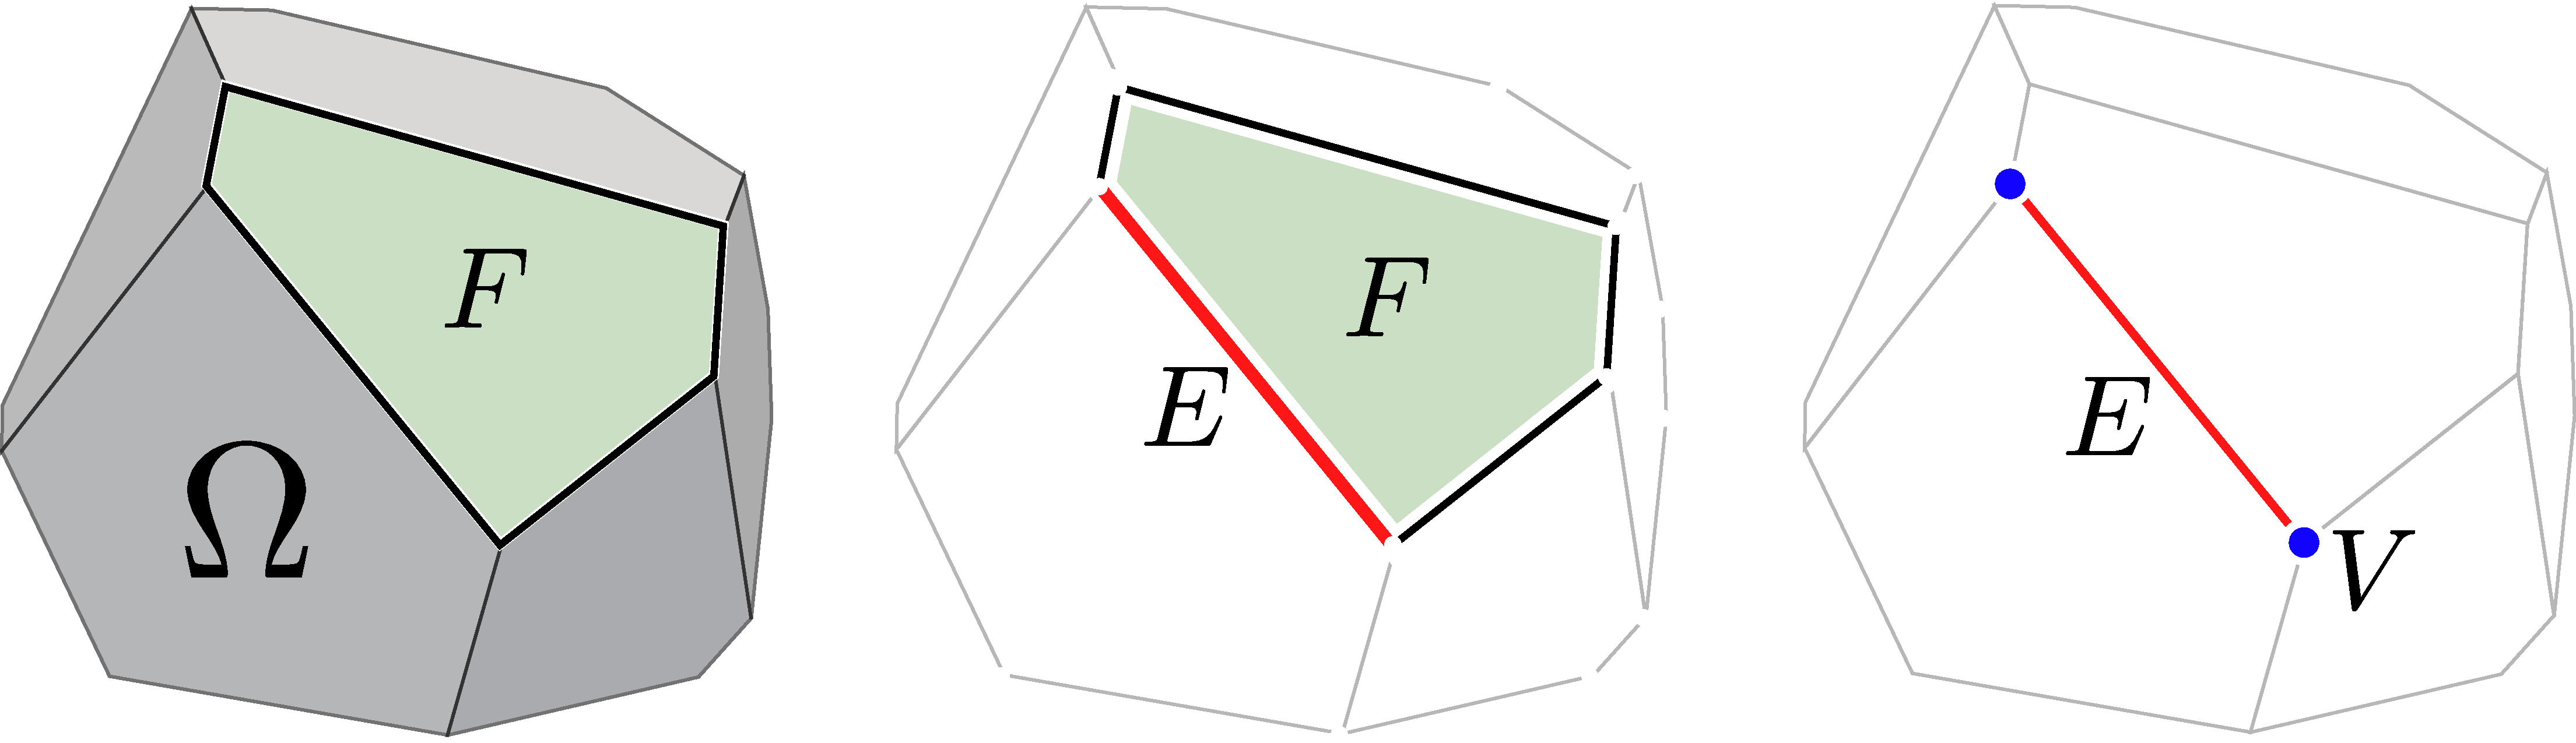
\includegraphics[width = 6.0in]{figures/polyhedron_decomposition.pdf}
	\caption{A representative polyhedral element $\Omega \subset \mathbb{R}^3$, a polygonal face $F \subset \partial \Omega$, a linear edge $E \subset \partial F$, and a node $V$.}
	\label{fig:polyhedral_element}
\end{figure}
	
	% PEM function spaces are broken $H^1 (\Omega)$ spaces
	% functions are defined independently on the open interior $\Omega$
	% functions defined independently on shared element interfaces
	The function spaces to which the element's shape functions are assumed to belong are broken Sobolev spaces, with a given shape function $\varphi \in \mathcal{W}_k (\overline{\Omega})$ defined independently on the open interior of each polyhedral element $\Omega \subset \mathbb{R}^3$, and on its boundary $\partial \Omega$, such that
	\begin{equation}
		\mathcal{W}_k (\overline{\Omega}) = \left\{ \varphi|_{\Omega} \in H^k (\Omega) : \mathcal{L}_{\Omega} \varphi = f_{\Omega} \, \text{in} \, \Omega, \, \varphi|_{F} \in \mathcal{W}_k (\overline{F}) \, \, \forall F \in \partial \Omega \right\},
	\end{equation}
	\begin{equation}
		\mathcal{W}_k (\overline{F}) = \left\{ \varphi|_{F} \in H^k (F) : \mathcal{L}_{F} \varphi = f_{F} \, \text{in} \, F, \, \varphi|_{E} \in \mathcal{W}_k (\overline{E}) \, \, \forall E \in \partial F \right\},
	\end{equation}
	\begin{equation}
		\mathcal{W}_k (\overline{E}) = \left\{ \varphi|_{E} \in H^k (E) : \mathcal{L}_{E} \varphi = f_{E} \, \text{in} \, E, \, \varphi|_{V} \in \mathbb{R} \, \, \forall V \in \partial E \right\}.
	\end{equation}
	In essence, a given function $\varphi|_{\Omega} \in H^k (\Omega)$ defined on the element's interior is related to a corresponding boundary function $\varphi|_{\partial \Omega} \equiv \bar{\varphi}$ (which itself is a broken $H^k (\partial \Omega)$ function) via a well-posed Dirichlet boundary value problem:
	\begin{equation}
		\mathcal{L}_{\Omega} \varphi = f_{\Omega} \quad \forall \mathbf{X} \in \Omega \quad \text{s.t.} \quad \varphi = \bar{\varphi} \quad \forall \mathbf{X} \in \partial \Omega,
		\label{eq:pem_bvp}
	\end{equation}
	where $\mathcal{L}_{\Omega}$ denotes a linear differential operator, and $f_{\Omega} \in L^2 (\Omega)$ is a generic forcing function. The element's degrees of freedom are collectively accounted for in the boundary function $\bar{\varphi}$, and in the forcing function $f_{\Omega}$. Consequently, the interior function $\varphi|_{\Omega}$ is uniquely defined, provided there exists a unique solution to (\ref{eq:pem_bvp}). In turn, we suppose that $\varphi|_{F} \in H^k(F)$ is the solution to a similar (2-dimensional) boundary value problem defined on each face $F$, and $\varphi|_E \in H^k(E)$ is the solution to a (1-dimensional) BVP on each edge $E$.
	
	% Additionally, the PEM considers the boundary of each element to be partitioned into a collection of $2$-dimensional polygonal faces $\partial \Omega = \cup_{i = 1}^{N_F} F_i$, where a given face $F$ is either a shared interface between two elements $F = \partial \Omega_a \cap \partial \Omega_b \neq \emptyset$ ($a \neq b$), or else it is a part of the domain boundary $F \subset \partial \Omega_a \cap \partial \mathcal{B}_0 \neq \emptyset$.
	% The boundary of each face $\partial F$ is likewise recursively partitioned into $1$-dimensional edges $\partial F = \cup_{i = 1}^{N_E} E_i$, whose end-points are the geometric verticies (the nodes) of the polyhedral element in question, which bear the primary degrees of freedom.
	
	The advantage of defining shape functions in this manner is that it affords a great deal of flexibility in the construction of arbitrary order interpolants (or enhancement functions), while maintaining $C^0 (\mathcal{B}_0)$ continuity at inter-element interfaces. Moreover, given that the shape functions are uniquely defined at every point $\mathbf{X} \in \overline{\Omega}$, they can be made amenable to post-processing and visualization-related tasks, if so desired.
	
%	In the following sections, we will explore a few specific choices for the differential operator $\mathcal{L}$ and the forcing functions $f$ defined on the element and its faces, etc.

\subsection*{Harmonic Shape Functions}

	% Ideally want the shape functions to be uniquely defined on polytopes
	% This can be achieved by considering SFs as unique solutions to BVPs
	% Most natural BVP to consider is Laplace's equation with Dirichlet BCs
	% BCs arise from conditions of compatibility with nodal values
		% Help to guarantee weak inter-element compatibility
	% Other authors have explored the idea of harmonic SFs on polytopes
		% See \cite{Gordon:74}, \cite{Martin:08}, \cite{Bishop:14}
		% To obtain these SFs, the authors use an element partition
	% In previous works, the BCs were enforced as closely as possible
	% This is not necessarily a good thing
		% The solution to Laplace's equation can yield sharp gradients
		% On arbitrary domains, can result in poor conditioning, locking
	% In the present work, we seek to relax the conditions of compatibility
		% Consider weak compatibility requirements
			% Develop notion of weak compatibility in a rigorous setting
			% Establish weak compatibility as sufficient for convergence
			% Examine necessary conditions for stability
		% Yields a non-conforming finite element method
		% Elements are more robust on account of relaxed compatibility
		% Polytopes accomodate nonconformity better (than simplicies, etc)

	The simplest choice of $\mathcal{L}_{\Omega} = -\nabla^2$ and $f_{\Omega} = 0$ corresponds to Laplace's equation:
	\begin{equation}
		\nabla^2 \varphi = 0 \quad \forall \mathbf{X} \in \Omega \quad \text{s.t.} \quad \varphi = \bar{\varphi} \quad \forall \mathbf{X} \in \partial \Omega,
		\label{eq:pem_laplace}
	\end{equation}
	whose solution $\varphi$ is harmonic on $\Omega$ (and likewise on each face $F$ and edge $E$ -- refer to Figure \ref{fig:harmonic_sfs}). Harmonic shape functions form a partition of unity, satisfy linear completeness, and arise from degrees of freedom borne only by the nodes of each element (i.e. the nodal values $\varphi|_V$); therefore, they satisfy the Kronecker delta property. As such, harmonic shape functions constitute a class of generalized barycentric coordinates.
	
\begin{figure} [!ht]
	\centering
	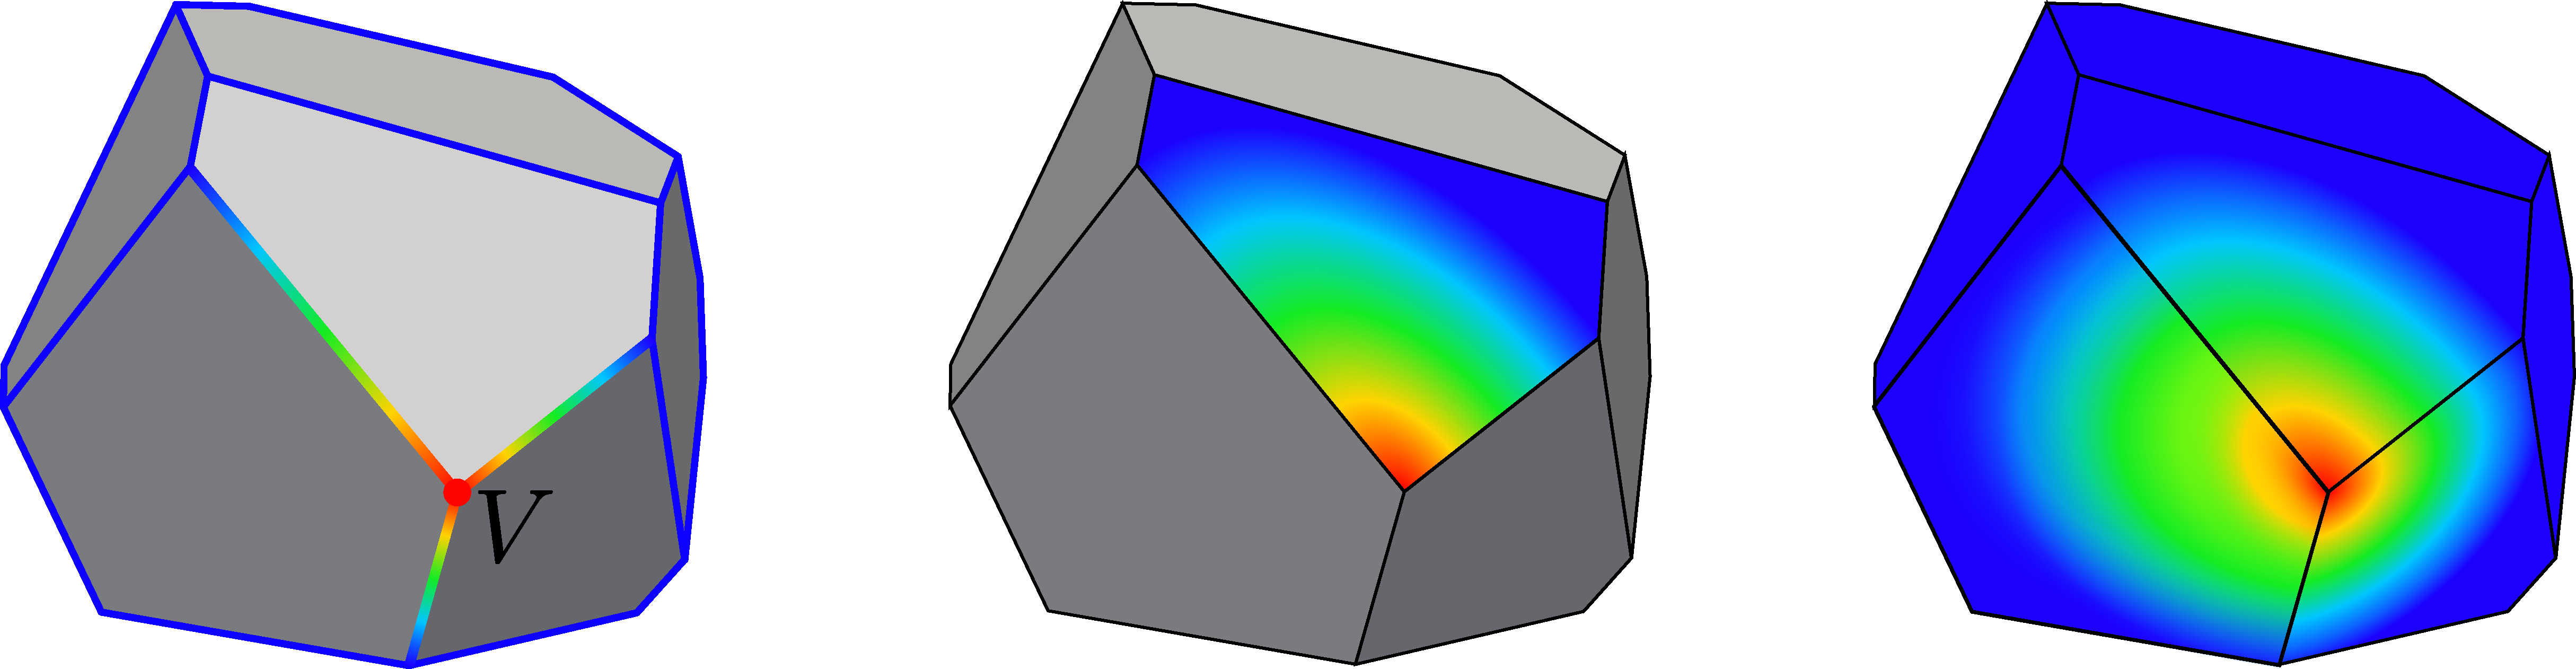
\includegraphics[width = 6.0in]{figures/harmonic_sfs.pdf}
	\caption{The harmonic shape function corresponding to the indicated node $V$, defined hierarchically on each edge, face, and the element.}
	\label{fig:harmonic_sfs}
\end{figure}
	
	If instead $f_{\Omega} \neq 0$ (corresponding to Poisson's equation), then
	\begin{equation}
		-\nabla^2 \varphi = f_{\Omega} \quad \forall \mathbf{X} \in \Omega \quad \text{s.t.} \quad \varphi = \bar{\varphi} \quad \forall \mathbf{X} \in \partial \Omega,
		\label{eq:pem_poisson}
	\end{equation}
	and we may introduce additional degrees of freedom through $f_{\Omega}$ belonging to the element (or its edges, faces). These degrees of freedom are effectively equivalent to bubble/enrichment functions; they are not directly associated with nodal evaluations of $\varphi$, but may be designed to exhibit certain desirable characteristics (e.g. to recover a particular order of polynomial completeness). The corresponding solution to (\ref{eq:pem_poisson}) is not harmonic; instead, we shall refer to functions which satisfy (\ref{eq:pem_poisson}) as \textit{generalized harmonic shape functions}.
	
	Harmonic shape functions are not a new concept; Gordon and Wixom were among the first authors to propose the idea in \cite{Gordon:74}, and Martin et al. later considered their application to polyhedral finite elements in \cite{Martin:08}. However, obtaining exact solutions to (\ref{eq:pem_laplace}) is generally infeasible for arbitrary polyhedra. In practice, approximate solutions must be considered.
	
	In particular, Bishop has proposed a method for constructing FE approximations to harmonic shape functions in \cite{Bishop:14}. Additionally, the VETFEM (\cite{Rashid:00}, \cite{Rashid:06}) and the original PEM presented in \cite{Rashid:12}, may be viewed as techniques for obtaining discrete approximations to harmonic shape functions. Likewise, many virtual element methods (\cite{Chi:17}, \cite{Veiga:13}, \cite{Veiga:15}) suppose that the element shape functions are harmonic over individual element domains, though they are never explicitly constructed or represented as such.

	Harmonic shape functions are desirable because they are uniquely defined, and therefore guarantee ellipticity of the resulting PEM systems of equations (discussed momentarily). However, polytopal finite element methods which employ harmonic shape functions may succumb to excessive interpolation errors for certain element shapes \cite{Gillette:16}. In particular, elements with non-convex features may severely degrade the convergence properties of such methods. An exploration of other forms for the elements' shape functions (possibly arising from a different choice of elliptic operator $\mathcal{L}$) is warranted. Nonetheless, in what follows, partitioned element methods based upon harmonic shape functions are deemed representative of a broader class of methods, which are likewise amenable to the developments considered herein.
	
	It therefore becomes of interest to determine suitable approximations to harmonic shape functions on arbitrary polyhedra. A number of methods to achieve this end are subsequently discussed.
	
\section{Shape Function Approximation Methods} \label{sec:approximations}
	
	The exact solution $\varphi \in \mathcal{U} (\Omega) = \left\{ \varphi \in H^1(\Omega) : \varphi = \bar{\varphi} \, \forall \mathbf{X} \in \partial \Omega \right\}$ to Poisson's equation in (\ref{eq:pem_poisson}) (or Laplace's equation in (\ref{eq:pem_laplace}) when $f_\Omega \equiv 0$) also satisfies the equivalent weak form:
	\begin{equation}
		\int_\Omega (\nabla^2 \varphi + f_{\Omega}) \eta \, dV = 0 \quad \forall \eta \in \mathcal{U}_0 (\Omega),
		\label{eq:initial_weak}
	\end{equation}
	or
	\begin{equation}
		\int_\Omega \nabla \varphi \cdot \nabla \eta \, dV = \int_\Omega f_{\Omega} \, \eta \, dV \quad \forall \eta \in \mathcal{U}_0 (\Omega),
		\label{eq:weak_bvp}
	\end{equation}
	where $\mathcal{U}_0 (\Omega) = \left\{ \eta \in H^1(\Omega) : \eta = 0 \, \forall \mathbf{X} \in \partial \Omega \right\}$ denotes an appropriately defined space of admissible variations.
	
	A vast array of different variational methods may be employed to obtain an approximate solution $\varphi^h \in \mathcal{U}^h (\Omega)$ satisfying
	\begin{equation}
		\int_\Omega \nabla \varphi^h \cdot \nabla \eta^h \, dV = \int_\Omega f_{\Omega} \, \eta^h \, dV \quad \forall \eta^h \in \mathcal{U}^h_0 (\Omega),
		\label{eq:approximate_bvp}
	\end{equation}
	where $\mathcal{U}^h (\Omega)$ and $\mathcal{U}^h_0 (\Omega)$ are taken to be finite-dimensional approximation spaces. Consequently, it is of interest to determine the essential requirements placed upon a given approximation $\varphi^h$ for the purposes of evaluating weak form integrals.
	
	Specifically, for a finite element approximation to the model problem given in (\ref{eq:bilinear_form}), consider the evaluation of an element's local bilinear form $a_{\Omega}(\mathbf{u},\mathbf{v})$, where $\mathbf{u} = \sum_{a=1}^N \varphi_a \mathbf{u}_a$ and $\mathbf{v} = \sum_{a=1}^N \varphi_a \mathbf{v}_a$ are written in terms of the element's shape functions $\left\{ \varphi_a \right\}_{a=1}^N$. An approximate evaluation of $a_{\Omega}(\mathbf{u},\mathbf{v})$ is obtained by making the substitution $a_{\Omega}(\mathbf{u}^h,\mathbf{v}^h)$, where $\mathbf{u}^h = \sum_{a=1}^N \varphi^h_a \mathbf{u}_a$ and $\mathbf{v}^h = \sum_{a=1}^N \varphi^h_a \mathbf{v}_a$ are instead represented in terms of the approximations $\left\{ \varphi^h_a \right\}_{a=1}^N$ to the element's shape functions.
	
	According to the virtual element decomposition proposed in \cite{Veiga:13}, we may express a given function $\mathbf{u} = \Pi^{\Omega}_k \mathbf{u} + (\mathbf{u} - \Pi^{\Omega}_k \mathbf{u})$ in terms of a low-order polynomial part $(\Pi^{\Omega}_k \mathbf{u})$ (up to degree $k$) and a non-polynomial part $(\mathbf{u} - \Pi^{\Omega}_k \mathbf{u})$, where $\Pi^{\Omega}_k : L^2 (\Omega) \mapsto P^k (\Omega)$ is a corresponding polynomial projection operator satisfying $a_{\Omega}(\Pi^{\Omega}_k \mathbf{u},\mathbf{v} - \Pi^{\Omega}_k \mathbf{v}) = 0 \, \, \forall \mathbf{u}, \mathbf{v}$, and thus
	\begin{equation}
		a_{\Omega}(\mathbf{u},\mathbf{v}) = a_{\Omega}(\Pi^{\Omega}_k \mathbf{u},\Pi^{\Omega}_k \mathbf{v}) + a_{\Omega}(\mathbf{u} - \Pi^{\Omega}_k \mathbf{u},\mathbf{v} - \Pi^{\Omega}_k \mathbf{v}).
		\label{eq:vem_decomposition}
	\end{equation}
	The first term appearing in the right-hand side of (\ref{eq:vem_decomposition}) accounts for the consistency of the finite element approximation, whereas the second term provides stability. To maintain consistency, the first term must be computed exactly, to the extent that
	\begin{equation}
		a_{\Omega}(\Pi^{\Omega}_k \mathbf{u},\Pi^{\Omega}_k \mathbf{v}) = a_{\Omega}(\Pi^{\Omega}_k \mathbf{u}^h,\Pi^{\Omega}_k \mathbf{v}^h),
	\end{equation}	
	yielding the $k-$consistency property:
	\begin{equation}
		a_{\Omega}(\Pi^{\Omega}_k \mathbf{u}^h,\mathbf{v}^h) = a_{\Omega}(\Pi^{\Omega}_k \mathbf{u},\mathbf{v}) \quad \forall \mathbf{v} \in \mathcal{V}^h (\Omega).
	\end{equation}
	However, the second term need only be sufficiently well-approximated by
	\begin{equation}
		a_{\Omega}(\mathbf{u} - \Pi^{\Omega}_k \mathbf{u},\mathbf{v} - \Pi^{\Omega}_k \mathbf{v}) \approx a_{\Omega}(\mathbf{u}^h - \Pi^{\Omega}_k \mathbf{u}^h,\mathbf{v}^h - \Pi^{\Omega}_k \mathbf{v}^h),
	\end{equation}
	to the extent that the correct order of convergence is maintained, and the inf-sup condition is altogether satisfied. In \cite{Veiga:13}, this is characterized by the assertion that there exist two positive constants $a_*$ and $a^*$ which are independent of the chosen discretization, such that the following stability condition holds:
	\begin{equation}
			a_* a_{\Omega} (\mathbf{v},\mathbf{v}) \leq a_{\Omega} (\mathbf{v}^h,\mathbf{v}^h) \leq a^* a_{\Omega} (\mathbf{v},\mathbf{v}) \quad \forall \mathbf{v} \in \mathcal{V}^h (\Omega).
	\end{equation}
	It is argued that these conditions are necessary and sufficient to guarantee convergence of the resulting method when the local approximations $\mathbf{u}^h$ and $\mathbf{v}^h$ are used in place of $\mathbf{u}$ and $\mathbf{v}$.
	
	It should be remarked that the evaluation of $a_{\Omega}(\mathbf{u},\mathbf{v})$ will be further approximated through the use of numerical quadrature on $\Omega$, herein denoted as $a^h_{\Omega}(\mathbf{u},\mathbf{v})$. Alternatively, the use of low-order quadrature rules may be viewed as an exact integration of corresponding low-order approximations to $\mathbf{u}$ and $\mathbf{v}$, i.e. $\exists \, \mathbf{u}^h,\mathbf{v}^h$ such that $a^h_{\Omega}(\mathbf{u},\mathbf{v}) = a_{\Omega}(\mathbf{u}^h,\mathbf{v}^h)$. The use of a numerical quadrature scheme is therefore subject to the conditions previously described.
	
	With the above considerations borne in mind, we propose a set of minimal requirements on the resulting approximations $\mathbf{u}^h$ and $\mathbf{v}^h$, and their corresponding integration via an appropriately defined quadrature rule:
	\begin{itemize}
		\item[(I)] $a^h_{\Omega}(\Pi^{\Omega}_k \mathbf{u}^h,\mathbf{v}^h) = a_{\Omega}(\Pi^{\Omega}_k \mathbf{u},\mathbf{v}) \quad \forall \mathbf{v} \in \mathcal{V}^h (\Omega)$.
		\item[(II)] $a_* a_{\Omega} (\mathbf{v},\mathbf{v}) \leq a^h_{\Omega} (\mathbf{v}^h,\mathbf{v}^h) \leq a^* a_{\Omega} (\mathbf{v},\mathbf{v}) \quad \forall \mathbf{v} \in \mathcal{V}^h (\Omega).$
	\end{itemize}
	
	An important distinction should be made with regard to the requirements placed upon a given variational method used to construct approximations $\varphi^h$ to (generalized) harmonic shape functions $\varphi$: it is not strictly necessary for the approximations to converge to $\varphi$ as the dimension of $\mathcal{U}^h (\Omega)$ is systematically increased. Provided the above conditions are met, convergence of the overarching finite element method is altogether achieved, even if relatively coarse/low-order approximations to the shape functions are utilized. Moreover, relaxing the requirements placed upon the approximations (particularly with regard to continuity) can have advantageous side-effects: the resulting finite element solution is made less sensitive to the choice of discretization, and poor stiffness matrix conditioning for elements with non-convex or degenerate features can be partially ameliorated. These considerations are investigated further in chapter \ref{ch:results}.
	
	The above considerations have prompted an investigation into the use of (discontinuous) low-order polynomial approximations to harmonic shape functions. These approximations are discussed in the following section.
	
\section{Non-conforming Galerkin Approximations to \\ (Generalized) Harmonic Shape Functions} \label{sec:nonconforming}

	If the boundary conditions imposed upon a given shape function are relaxed to the extent that $\varphi^h \neq \bar{\varphi}$ on $\partial \Omega$, then clearly $\mathcal{U}^h (\Omega) \not\subset \mathcal{U} (\Omega)$, and one must resort to the use of non-conforming approximation methods to obtain suitable approximations $\varphi^h$. In such cases, the boundary conditions must be imposed in a weak sense, such that $\varphi^h$ still yields satisfaction of conditions (I) and (II), as developed in the previous section.
	
	A number of weak enforcement strategies for the Dirichlet boundary condition ($\varphi = \bar{\varphi}$ on $\partial \Omega$) are suggested in the following sections.
	
	\subsection*{Weak Enforcement of Boundary Conditions via a Lagrange Multiplier Method}
	
	One approach to weakly enforce the boundary condition $\varphi = \bar{\varphi}$ on $\partial \Omega$ would be to consider a Lagrange multiplier method, wherein
	\begin{equation}
		\min_{\varphi, \, \lambda} \mathcal{L}(\varphi,\lambda),
	\end{equation}
	\begin{equation}
	\mathcal{L}(\varphi,\lambda) \equiv \frac{1}{2} \int_{\Omega} \nabla \varphi \cdot \nabla \varphi \, dV - \int_{\Omega} f_{\Omega} \, \varphi \, dV + \int_{\partial \Omega} \left[ \varphi - \bar{\varphi} \right] \lambda \, dA,
\end{equation}
	involving the specification of a Lagrange multiplier field $\lambda \in \Lambda (\partial \Omega) = \left\{ \lambda \in L^2 (\partial \Omega) \right\}$, and its corresponding discrete approximation $\lambda^h \in \Lambda^h (\partial \Omega) \subset \Lambda (\partial \Omega)$. Taking the first variation of the Lagrangian yields two sets of equations in terms of the approximations $\varphi^h \in \mathcal{U}^h (\Omega)$ and $\lambda^h \in \Lambda^h (\partial \Omega)$:
	\begin{equation}
		\int_{\Omega} \nabla \varphi^h \cdot \nabla \eta^h \, dV - \int_\Omega f_\Omega \eta^h \, dV + \int_{\partial \Omega} \lambda^h \eta^h \, dA = 0 \quad \forall \eta^h \in \mathcal{U}^h (\Omega),
	\end{equation}
	\begin{equation}
		\int_{\partial \Omega} (\varphi^h - \bar{\varphi}) \, \mu^h \, dA = 0 \quad \forall \mu^h \in \Lambda^h (\partial \Omega).
	\end{equation}
	Suppose finite-dimensional bases are established for $\mathcal{U}^h (\Omega)$ and $\Lambda^h (\partial \Omega)$, i.e.
\begin{equation}
	\varphi^h (\mathbf{X}) = \sum_{a=1}^{N} \psi_a (\mathbf{X}) \varphi_a, \quad \lambda^h (\mathbf{X}) = \sum_{a=1}^{M} \chi_a (\mathbf{X}) \lambda_a,
\end{equation}
such that
\begin{equation}
	\sum_{a=1}^N \left[ \int_{\Omega} \nabla \psi_a \cdot \nabla \psi_b \, dV \right] \varphi_a + \sum_{c=1}^M \left[ \int_{\partial \Omega} \psi_b \, \chi_c \, dA \right] \lambda_c = \int_{\partial \Omega} f_\Omega \, \psi_b \, dA \quad \forall b,
\end{equation}
\begin{equation}
	\sum_{b=1}^N \left[ \int_{\partial \Omega} \chi_c \, \psi_b \, dA \right] \varphi_b = \int_{\partial \Omega} \bar{\varphi} \, \chi_c \, dA \quad \forall c.
\end{equation}
Given an appropriate selection for the indicated bases, the determination of the unknowns ($\varphi_a$ and $\lambda_a$) entails the solution of a saddle-point system of equations, written in matrix-vector format:
\begin{equation}
	\left[ \begin{array}{cc} \mathbf{A} & \mathbf{B} \\ \mathbf{B}^T & \mathbf{0} \end{array} \right] \left\{ \begin{array}{c} \boldsymbol{\varphi} \\ \boldsymbol{\lambda} \end{array} \right\} = \left\{ \begin{array}{c} \mathbf{f} \\ \bar{\boldsymbol{\varphi}} \end{array} \right\},
\end{equation}
where
\begin{equation}
	A_{ab} = \int_{\Omega} \nabla \psi_a \cdot \nabla \psi_b \, dV, \quad B_{bc} = \int_{\partial \Omega} \psi_b \, \chi_c \, dA,
\end{equation}
\begin{equation}
	f_{b} = \int_{\partial \Omega} f_\Omega \, \psi_b \, dA, \quad \bar{\varphi}_{c} = \int_{\partial \Omega} \bar{\varphi} \, \chi_c \, dA.
\end{equation}

	The main advantage of this approach is that virtually any space of functions may be selected for $\mathcal{U}^h (\Omega)$, such that the resulting approximations $\varphi^h \in \mathcal{U}^h (\Omega)$ can be made less sensitive to degenerate geometric features of the element (namely, short edges).
	
	Arguably the simplest (and most efficient) choice is $\mathcal{U}^h (\Omega) = P^{m} (\Omega)$ where $m \geq k$, resembling certain formulations of the VETFEM (\cite{Rashid:00}, \cite{Rashid:06}), where the basis functions for the Lagrange multiplier field are Dirac delta functions $\chi_c (\mathbf{X}) = \delta (\mathbf{X} - \mathbf{X}_c) \, \, \forall c = 1, \ldots, N_v$ associated with the individual nodes of the element. A potential shortcoming of this particular choice for $\chi_c$ is that the resulting shape functions may nonetheless possess sharp gradients in the vicinity of short element edges, leading to undesirable behavior -- poor numerical conditioning of the element's local stiffness matrix.
	
	Various other choices for the Lagrange multiplier basis are possible which may yield less spurious approximations (for instance $\Lambda^h (\partial \Omega) = P^{m} (\partial \Omega)$). However, careful attention must be paid to the selection of $\mathcal{U}^h (\Omega)$ and $\Lambda^h (\partial \Omega)$, as poorly chosen bases can lead to ill-posedness of the saddle-point problem. More sophisticated linear solution methodologies may be required in these cases.

	\subsection*{Weak Enforcement of Boundary Conditions via Nitsche's Method}
	
	As a viable alternative to the Lagrange multiplier method presented in the previous section, the boundary conditions may be enforced weakly via Nitsche's method:
	\begin{eqnarray}
		\int_{\Omega} \nabla \varphi^h \cdot \nabla \eta^h \, dV + \int_{\partial \Omega} \left[ \epsilon \, \frac{\partial \eta^h}{\partial N} \varphi^h - \eta^h \, \frac{\partial \varphi^h}{\partial N} \right] \, dA + \frac{\alpha}{|\partial \Omega|^{\beta}} \int_{\partial \Omega} \varphi^h \eta^h \, dA \nonumber \\ = \int_\Omega f_\Omega \, \eta^h \, dV + \epsilon \int_{\partial \Omega} \frac{\partial \eta^h}{\partial N} \, \bar{\varphi} \, dA + \frac{\alpha}{|\partial \Omega|^{\beta}} \int_{\partial \Omega} \bar{\varphi} \, \eta^h \, dA \quad \forall \eta^h \in \mathcal{U}^h (\Omega),
		\label{eq:vetfem}
	\end{eqnarray}
	where $\alpha > 0$ is a stabilization parameter, $| \partial \Omega |$ denotes the surface area of $\partial \Omega$, and $\beta = (d-1)^{-1}$ for $\Omega \subset \mathbb{R}^d$, $d \geq 2$. The symmetric form of Nitsche's method \cite{Juntunen&Stenberg:09} corresponds to the case where $\epsilon = -1$, whereas the nonsymmetric form (\cite{Freund:95}, \cite{Burman:12}) corresponds to $\epsilon = +1$.
	
	Provided the stabilization parameter $\alpha$ is specified appropriately, the Galerkin approximation $\varphi^h$ can be obtained as the solution to a positive-definite system of equations: $\mathbf{A} \boldsymbol{\varphi} = \mathbf{f}$, where
	\begin{equation}
		A_{ab} = \int_{\Omega} \nabla \psi_a \cdot \nabla \psi_b \, dV + \int_{\partial \Omega} \left[ \epsilon \, \frac{\partial \psi_b}{\partial N} \psi_a - \psi_b \frac{\partial \psi_a}{\partial N} \right] \, dA + \frac{\alpha}{|\partial \Omega|^{\beta}} \int_{\partial \Omega} \psi_a \, \psi_b \, dA,
	\end{equation}
	\begin{equation}
		f_{b} = \int_{\Omega} f_\Omega \, \psi_b \, dV + \epsilon \int_{\partial \Omega} \frac{\partial \psi_b}{\partial N} \, \bar{\varphi} \, dA + \frac{\alpha}{|\partial \Omega|^{\beta}} \int_{\partial \Omega} \bar{\varphi} \, \psi_b \, dA.
	\end{equation}
	
	As discussed in the previous section, a rather natural choice for the space of approximating functions is $\mathcal{U}^h (\Omega) = P^{m} (\Omega)$ with $m \geq k$. The resulting method yields reasonably well-conditioned stiffness matrices for convex shapes, even when the elements possess degenerate edges. However, experimental evidence suggests that for non-convex shapes, the resulting shape function approximations may succumb to Runge's phenomenon, yielding highly oscillatory approximations. A more thorough investigation of this behavior is presented in chapter \ref{ch:results}.
	
	These observations have led to the conclusion that approximations consisting of piecewise polynomials may yield more well-behaved (less oscillatory) solutions for $\varphi^h$. The remainder of our discussion will focus upon such methods.
	
\section{Piecewise Polynomial Approximations to \\ (Generalized) Harmonic Shape Functions}

Partitioned element methods consider the approximation to a given element's shape functions via piecewise polynomials defined over a partition of the element's domain. In this regard, the approach proposed by Bishop in \cite{Bishop:14} is properly regarded as a partitioned element method which utilizes $C^0$ FE approximations to harmonic shape functions. In like fashion, the eponymous partitioned element method introduced in \cite{Rashid:12} utilizes weakly continuous piecewise polynomial approximations to harmonic shape functions. Herein we propose a novel alternative approach based upon the interior penalty discontinuous Galerkin finite element method (henceforth, the DG-PEM).

A few preliminary definitions regarding the element's partition are given, followed by a more thorough discussion of several partition-based approximation methods.

\subsection*{The Element Partition}

\begin{figure} [!ht]
	\centering
	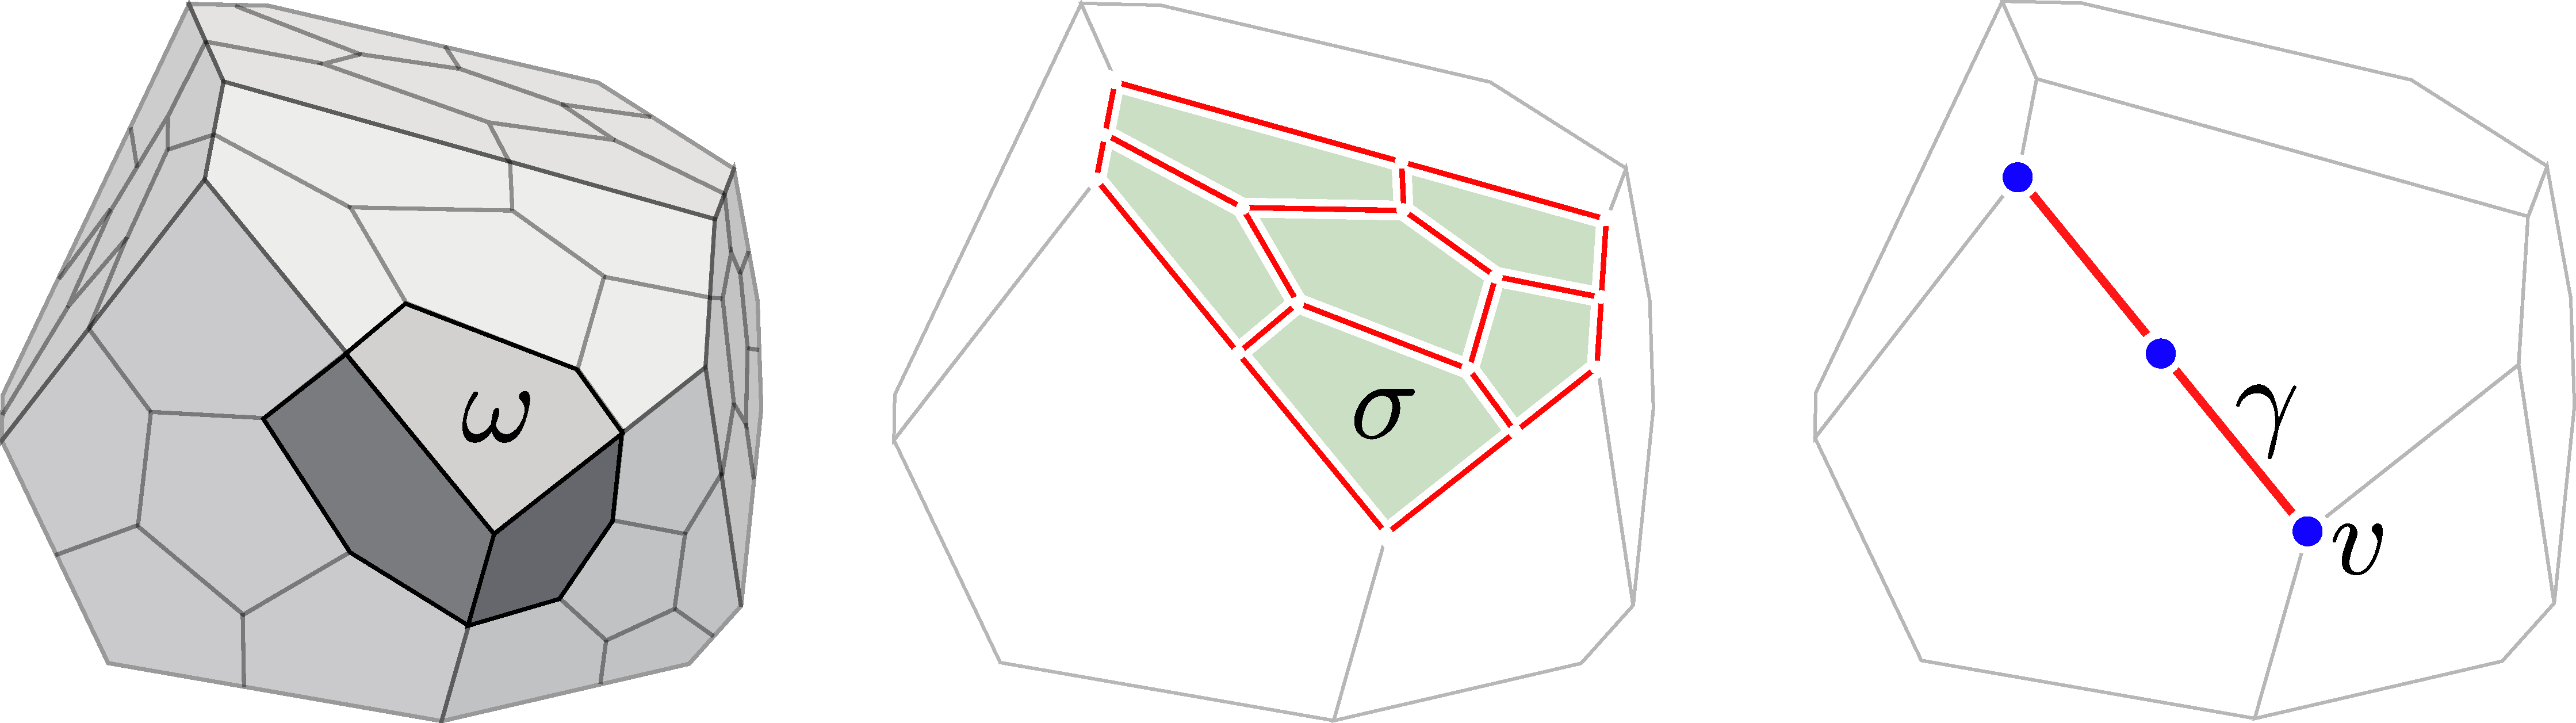
\includegraphics[width = 6.0in]{figures/polyhedron_partition.pdf}
	\caption{A representative polyhedral element $\Omega \subset \mathbb{R}^3$, and its hierarchical partition into cells, facets, segments, and vertices.}
	\label{fig:partitioned_element}
\end{figure}

	Consider a partition $\mathcal{T}_\omega (\Omega)$ of a given polyhedral element $\Omega$ into polyhedral cells $\omega \subset \Omega$. The boundary of each cell consists of polygonal facets $\sigma \subset \partial \omega$. Further, denote by $\Gamma_\omega$ the set of all interior cell interfaces (facets) shared by two adjacent cells, such that a given polygonal facet $\sigma$ belongs either to $\Gamma_\omega$, or to the boundary of the element $\partial \Omega$.
	
	In turn, let $\mathcal{T}_{\sigma} (F)$ denote the partition of a given face $F \subset \partial \Omega$ into polygonal facets $\sigma \subset F$. The boundary of each facet consists of linear segments $\gamma \subset \partial \sigma$. For a given face $F$, let $\Gamma_\sigma$ denote the set of all interior facet interfaces (segments) shared by two facets belonging to $F$, such that a given linear segment $\gamma$ belongs either to $\Gamma_\sigma$ or $\partial F$.
	
	Finally, $\mathcal{T}_{\gamma} (E)$ denotes the partition of a given edge $E \subset \partial F$ into linear segments $\gamma \subset E$. The endpoints of each segment are called vertices, denoted $v$. For a given edge $E$, denote by $\Gamma_\gamma$ the set of all interior segment interfaces (vertices) shared by two segments belonging to $E$, such that a given vertex $v$ belongs either to $\Gamma_\gamma$ or $\partial E$. As well, each node $V$ corresponds to a single vertex $v$, though not all vertices coincide with a node.
	
	A number of simple partitioning schemes are proposed, and illustrated in Figure \ref{fig:partitioning_types}:
	\begin{figure} [!ht]
		\centering
		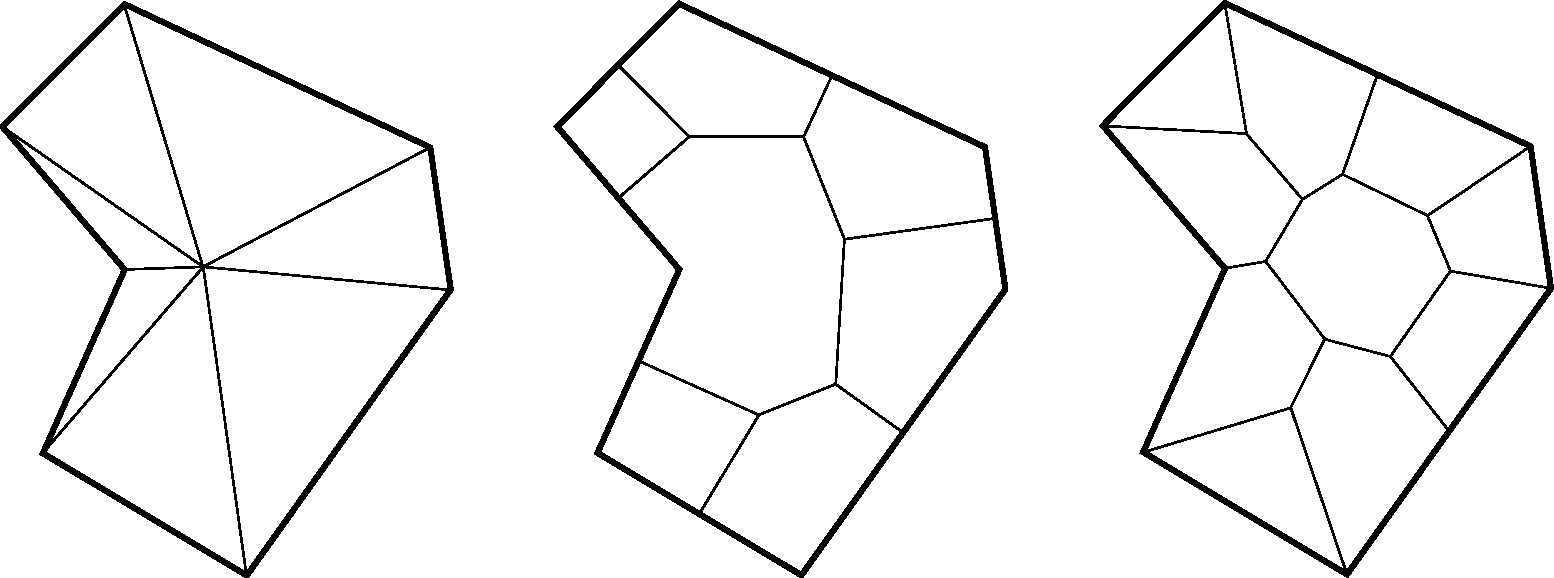
\includegraphics[width = 4.0in]{figures/partition_types.pdf}
		\caption{Polygonal element partitioning schemes: (top-left) edge-based partition, (top-right) node-based partition, (bottom-left) random Delaunay partition, (bottom-right) random Voronoi partition.}
		\label{fig:partitioning_types}
	\end{figure}
	\begin{itemize}
		\item \textbf{Edge-based}: For star-convex shapes -- the vertex-averaged centroid is used to subdivide the element into triangles (in 2D) or tetrahedra (in 3D) associated with each linear edge of the element.
		\item \textbf{Node-based}: For arbitrary shapes -- the element is sub-divided into quadrature cells corresponding to tributary regions surrounding each node.
		\item \textbf{Random Delaunay}: For arbitrary shapes -- the element is sub-divided into a Delaunay triangulation (in 2D) or tetrahedralization (in 3D), whose corresponding vertices are generated via a random point sampling process.
		\item \textbf{Random Voronoi}: For arbitrary shapes -- the element is sub-divided into Voronoi cells, whose corresponding voronoi sites are generated via a constrained maximal Poisson-disk sampling process, as described in \cite{Ebeida:11}.
	\end{itemize}
	
	We denote the volume of a given cell as $|\omega|$, the area of a facet as $|\sigma|$, and the length of a segment as $|\gamma|$. Each facet likewise possesses an associated normal direction $\mathbf{N}_\sigma$, whose orientation is outward from $\Omega$ for all $\sigma \in \partial \Omega$. For all $\sigma \in \Gamma_\omega$ shared by two cells ($\omega_1$ and $\omega_2$), the orientation of $\mathbf{N}_\sigma$ is outward with respect to $\omega_1$.
	
\subsection*{Continuous Galerkin Approximations to \\ (Generalized) Harmonic Shape Functions}

	Consider finite dimensional sub-spaces $\mathcal{U}^h (\Omega) \subset \mathcal{U} (\Omega)$ and $\mathcal{U}^h_0 (\Omega) \subset \mathcal{U}_0 (\Omega)$. The continuous Galerkin approximation $\varphi^h \in \mathcal{U}^h (\Omega)$ to a given (generalized) harmonic shape function $\varphi \in \mathcal{U} (\Omega)$ satisfies
	\begin{equation}
		\int_\Omega \nabla \varphi^h \cdot \nabla \eta^h \, dV = \int_\Omega f_{\Omega} \, \eta^h \, dV \quad \forall \eta^h \in \mathcal{U}^h_0 (\Omega).
		\label{eq:weak_poisson}
	\end{equation}

%	If $f_\Omega \equiv 0$ (yielding the harmonic shape functions), we may invoke the Galerkin orthogonality property to determine that the error $e = \varphi^h - \varphi$ in approximating $\varphi$ is orthogonal to $\mathcal{U}^h (\Omega)$, such that
%	\begin{equation}
%		\langle e, \eta^h \rangle = 0 \quad \forall \eta^h \in \mathcal{U}^h (\Omega),
%	\end{equation}
%	where $\langle u, v \rangle \equiv \int_\Omega \nabla u \cdot \nabla v \, dV$. Further, it may be remarked that for any two shape functions $\varphi_a, \varphi_b$, we obtain
%	\begin{equation}
%		\langle \varphi_a, \varphi_b \rangle = \langle \varphi^h_a + e_a, \varphi^h_b + e_b \rangle = \langle \varphi^h_a, \varphi^h_b \rangle + \langle e_a, e_b \rangle,
%	\end{equation}
%	owing to $\langle e_a, \varphi^h_b \rangle = \langle \varphi^h_a, e_b \rangle = 0$.
%
%	In effect, we may consider a given approximant $\varphi^h$ to be the $L^2(\Omega)$ projection of $\varphi$ onto $\mathcal{U}^h (\Omega)$ (a direct consequence of Galerkin orthogonality), which further implies that the evaluation of weak form integrals $a_\Omega (\mathbf{u}, \mathbf{v})$ are sufficiently well-approximated by their counterparts $a_\Omega (\mathbf{u}^h, \mathbf{v}^h)$. Indeed, if we make the substitution
%	\begin{equation}
%		a_\Omega (\mathbf{u}^h, \mathbf{v}^h) = \sum_{a=1}^N \sum_{b=1}^N  \mathbf{u}_a a_\Omega (  \varphi^h_a, \varphi^h_b ) \mathbf{v}_b,
%	\end{equation}
%	we would need to verify that $a_\Omega (  \varphi^h_a, \varphi^h_b )$ yields a sufficiently stable discrete operator. Satisfaction of the completeness requirements is guaranteed, so long as $\mathcal{U}^h (\Omega) \supset P^k(\Omega)$. It is not difficult to show that
%	\begin{equation}
%		a_\Omega (  \varphi^h_a, \varphi^h_a ) \leq a_\Omega (  \varphi_a, \varphi_a ).
%	\end{equation}
	
	Bishop has already explored such an approach in \cite{Bishop:14} for constructing approximations to harmonic shape functions using a partition of a given polyhedral element into sub-dividing tetrahedra. The approximation space $\mathcal{U}^h (\Omega)$ is spanned by $C^0 (\Omega)$ finite element basis functions defined on the tetrahedral partition of $\Omega$. The corresponding shape function approximations $\varphi^h \in \mathcal{U}^h (\Omega)$ are obtained as the solutions to a set of local finite element problems defined on $\Omega$ (and its faces, edges -- refer to Figure \ref{fig:harmonic_fem_sfs}). This approach will be distinguished as the \textit{continuous Galerkin partitioned element method} (CG-PEM).
	
\begin{figure} [!ht]
	\centering
	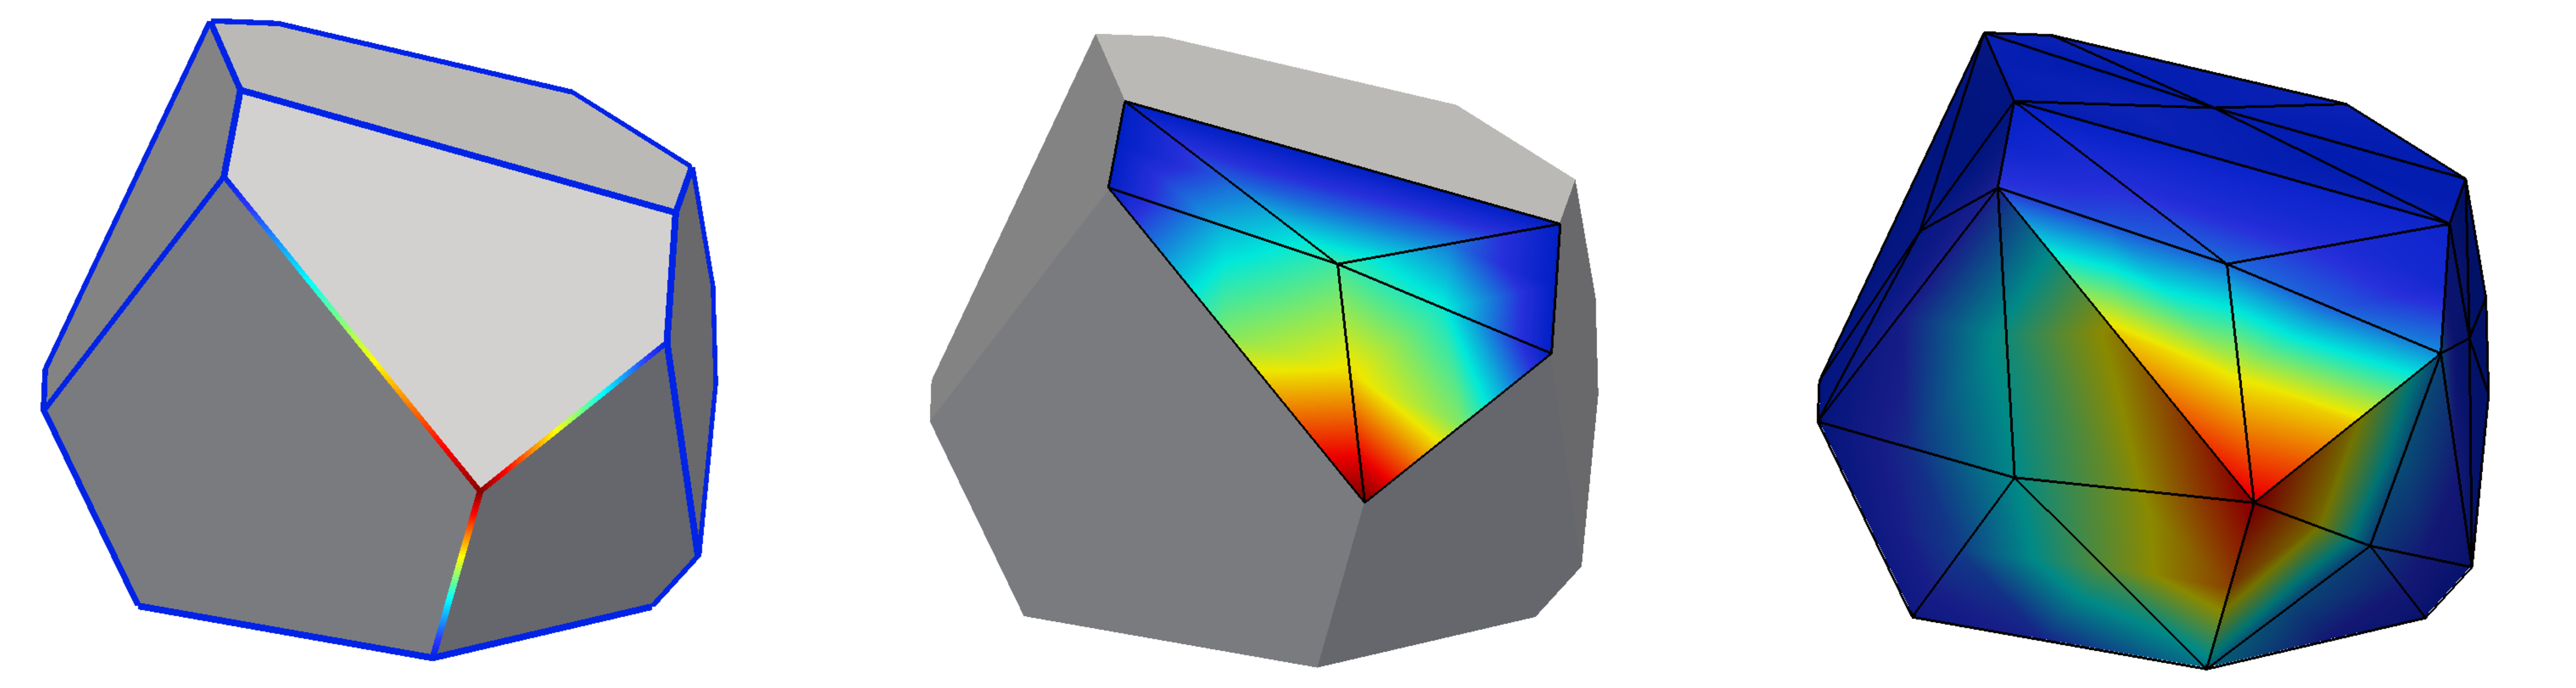
\includegraphics[width = 6.0in]{figures/harmonic_fem_sfs.pdf}
	\caption{The CG-PEM approximation to a given harmonic shape function, defined hierarchically on the element's faces and edges.}
	\label{fig:harmonic_fem_sfs}
\end{figure}
	
	It was demonstrated in \cite{Bishop:14} that the resulting approximations $\varphi^h$ preserve low-order polynomial completeness -- a direct consequence of $\mathcal{U}^h (\Omega) \supset P^1 (\Omega)$. If the elements are discretized into a sufficient number of tetrahedra, the method is observed to be stable. If sufficiently accurate quadrature rules are specified on $\Omega$ and $\partial \Omega$, the CG-PEM also yields a consistent integration of the weak form.
	
	For coarse tetrahedral sub-divisions, the local FE problems that must be solved on each element are relatively small, in some cases entailing only a single degree of freedom. However, the approach can become computationally expensive if the elements are subdivided into an excessively large number of tetrahedra (in the event that more accurate/refined approximations to the shape functions are desired). Initial numerical investigations conducted by Bishop have suggested that relatively coarse tetrahedral sub-divisions of the elements provide sufficiently accurate results; further subdivision (tetrahedral $h-$refinement) does little to improve the overall accuracy of the method.
	
	A natural extension of the method to higher-order serendipity elements would be to consider $p-$refinement of an element's tetrahedral subdivision to recover higher-order polynomial completeness, i.e. to guarantee $\mathcal{U}^h (\Omega) \supset P^k (\Omega)$ for some desired polynomial order $k$. The construction of shape functions on a given element would likely bear a much higher computational cost with increasing polynomial degree, owing to the increased size of the local FE problems on $\Omega$. Moreover, the specification of efficient yet stable and accurate numerical quadratures would present an additional challenge.
	
	The notion of subdividing the elements into conforming finite elements presents an obvious complication, however. The primary obstacle for traditional finite element methods is the process of obtaining a mesh. Requiring that the elements be partitioned into canonical finite elements does not obviate the meshing problem; it only defers the problem to the element formulation. Moreover, obtaining an FE partition for an arbitrary polyhedral element presents similar challenges to meshing a complicated problem domain. A separate generalization would be to consider subdividing the elements into arbitrary polyhedra, solving (\ref{eq:weak_poisson}) by means of the virtual element method. This would allow for a more natural collocation of quadrature cells with the specified subdivision, resembling the partitioned element method proposed in \cite{Rashid:12}.
	
	As will be discussed in chapter \ref{ch:results}, a particular complication arises for harmonic shape functions and their corresponding $C^0 (\Omega)$ approximations on irregularly shaped elements: the solution to Laplace's equation may possess extremely sharp gradients if the geometry of the element contains reflex corners or nearly degenerate features (i.e. short edges). A consequence of this is poor conditioning of the element's local stiffness matrix, leading to excessively stiff modes of deformation (locking), and issues of numerical conditioning in the linear solution process.
	
\subsubsection*{Integration Consistency of the CG-PEM}

	Consider the case when (\ref{eq:initial_weak}) is integrated against an arbitrary polynomial test function $\eta \in P^k (\Omega)$. Integrating by parts yields:
	\begin{equation}
		\int_\Omega \nabla \varphi \cdot \nabla \eta \, dV = \int_\Omega f_{\Omega} \, \eta \, dV + \int_{\Omega} \nabla \cdot (\eta \, \nabla \varphi) \, dV \quad \forall \eta \in P^k (\Omega).
	\end{equation}
	Note that
	\begin{equation}
		\int_\Omega \nabla \varphi \cdot \nabla \eta \, dV = \int_\Omega \left[ \nabla \cdot (\varphi \, \nabla \eta) - \varphi \, \nabla^2 \eta \right] \, dV \quad \forall \eta \in P^k (\Omega),
	\end{equation}
	and the boundary condition ($\varphi = \bar{\varphi}$ on $\partial \Omega$) implies
	\begin{equation}
		\int_\Omega \nabla \cdot (\varphi \, \nabla \eta) \, dV = \int_{\partial \Omega} (\mathbf{N} \cdot \nabla \eta) \, \bar{\varphi} \, dA \quad \forall \eta \in P^k (\Omega).
	\end{equation}
	Thus:
	\begin{equation}
		\int_{\partial \Omega} (\mathbf{N} \cdot \nabla \eta) \, \bar{\varphi} \, dA = \int_\Omega \left[ \varphi \, \nabla^2 \eta + f_{\Omega} \, \eta \right] \, dV + \int_{\Omega} \nabla \cdot (\eta \, \nabla \varphi) \, dV \quad \forall \eta \in P^k (\Omega).
	\end{equation}
	Additionally, noting that $\nabla \cdot (\eta \nabla \varphi) = \nabla \varphi \cdot \nabla \eta + \eta \, \nabla^2 \varphi$, we observe that
	\begin{equation}
		\int_{\Omega} \left[ \nabla \varphi \cdot \nabla \eta + \varphi \, \nabla^2 \eta \right] \, dV - \int_{\partial \Omega} (\mathbf{N} \cdot \nabla \eta) \, \bar{\varphi} \, dA = \int_\Omega (\nabla^2 \varphi + f_{\Omega}) \, \eta \, dV \quad \forall \eta \in P^k (\Omega),
	\end{equation}
	which necessitates that the following expression hold for all $\eta \in P^k (\Omega)$:
	\begin{equation}
		\int_{\Omega} \nabla \varphi \cdot \nabla \eta \, dV + \int_{\Omega} \varphi \, \nabla^2 \eta \, dV = \int_{\partial \Omega} (\mathbf{N} \cdot \nabla \eta) \, \bar{\varphi} \, dA \quad \forall \eta \in P^k (\Omega).
	\end{equation}
	
	Consider a finite element approximation space $\mathcal{U}^h (\Omega) \supset P^k (\Omega)$ defined on a corresponding partition $\mathcal{T}_\omega (\Omega)$ of $\Omega$. The above expression implies that the approximate solution $\varphi^h \in \mathcal{U}^h (\Omega) \subset \mathcal{U} (\Omega)$ to (\ref{eq:weak_poisson}) satisfies the integration consistency conditions:
	\begin{equation}
		\int_{\Omega} \mathbf{v} \cdot \nabla \varphi^h \, dV + \int_{\Omega} \varphi^h \, \nabla \cdot \mathbf{v} \, dV = \int_{\partial \Omega} \mathbf{v} \cdot \mathbf{N} \, \bar{\varphi} \, dA \quad \forall \mathbf{v} \in \left[ P^{(k-1)} (\Omega) \right]^d,
		\label{eq:cg_pem_integration_consistency}
	\end{equation}
	where $\mathbf{v} = \nabla \eta$ for some $\eta \in P^k (\Omega)$. If (\ref{eq:cg_pem_integration_consistency}) is integrated exactly by the element's quadrature rules, the resulting CG-PEM elements will pass finite element patch tests up to k$^{\text{th}}$ order. If the element's partition consists of linear triangles and tetrahedra, a composite mid-point quadrature scheme proves to be sufficient to this end.

\subsection*{Discontinuous Galerkin Approximations to \\ (Generalized) Harmonic Shape Functions}

	Consider the broken Sobolev space $\mathcal{D}^h_k (\Omega) = \left\{ \varphi \in L^2 (\Omega) : \varphi|_{\omega} \in P^k (\omega) \, \forall \omega \in \mathcal{T}_\omega (\Omega) \right\}$ consisting of (discontinuous) piecewise polynomials defined over the partition of the element. Herein, the family of interior penalty discontinuous Galerkin methods described in \cite{Riviere:08} are applied to (\ref{eq:weak_bvp}). In doing so, one obtains piecewise discontinuous approximations to generalized harmonic shape functions $\varphi^h \in \mathcal{D}^h_k (\Omega) \not\subset \mathcal{U} (\Omega)$. The reader is cautioned against several apparent errors in the presentation of interior penalty DG methods found in \cite{Riviere:08}. The following weak form is consistent with \cite{Riviere:01}:
	\begin{eqnarray}
		\sum_{\omega \in \mathcal{T}_\omega (\Omega)} \int_{\omega} \nabla \varphi^h \cdot \nabla \eta^h \, dV + \sum_{\sigma \in \Gamma_\omega \cup \partial \Omega} \int_{\sigma} \bigg( \epsilon \left\{ \frac{\partial \eta^h}{\partial N_{\sigma}} \right\} [\![ \varphi^h ]\!] - [\![ \eta^h ]\!] \left\{ \frac{\partial \varphi^h}{\partial N_{\sigma}} \right\}  \bigg) \, dA \nonumber \\ + J_0 (\varphi^h,\eta^h) + J_1 (\varphi^h,\eta^h) = \int_{\Omega} f_{\Omega} \, \eta^h \, dV + \sum_{\sigma \in \partial \Omega} \int_{\sigma} \left(\frac{\alpha_{\sigma0}}{|\sigma|^{\beta_0}} \eta^h + \epsilon \frac{\partial \eta^h}{\partial N_{\sigma}} \right) \bar{\varphi} \, dA
		\label{eq:dg_poisson}
	\end{eqnarray}
	for all $\eta^h \in \mathcal{D}^h_k (\Omega)$, where
	\begin{equation}
		\{ \varphi \} = \frac{1}{2} (\varphi|_{\omega_1} + \varphi|_{\omega_2}), \quad [\![ \varphi ]\!] = (\varphi|_{\omega_1} - \varphi|_{\omega_2}) \quad \forall \sigma = \partial \omega_1 \cap \partial \omega_2,
		\label{eq:internal_jumps}
	\end{equation}
	\begin{equation}
		\{ \varphi \} = [\![ \varphi ]\!] = \varphi|_{\omega} \quad \forall \sigma = \partial \omega \cap \partial \Omega,
		\label{eq:external_jumps}
	\end{equation}
	The supplementary bilinear forms $J_0 (\varphi^h,\eta^h)$ and $J_1 (\varphi^h,\eta^h)$ are defined as:
	\begin{equation}
		J_0 (\varphi^h,\eta^h) = \sum_{\sigma \in \Gamma_\omega \cup \partial \Omega} \frac{\alpha_{\sigma0}}{|\sigma|^{\beta_0}} \int_{\sigma} [\![ \varphi^h ]\!] \, [\![ \eta^h ]\!] \, dA,
	\end{equation}
	\begin{equation}
		J_1 (\varphi^h,\eta^h) = \sum_{\sigma \in \Gamma_\omega} \frac{\alpha_{\sigma1}}{|\sigma|^{\beta_1}} \int_{\sigma} \left[\!\!\left[ \frac{\partial \varphi^h}{\partial N_{\sigma}} \right]\!\!\right] \, \left[\!\!\left[ \frac{\partial \eta^h}{\partial N_{\sigma}} \right]\!\!\right] \, dA.
	\end{equation}
	These two terms penalize jumps in the indicated functions' values and their normal derivatives at cell boundaries, respectively. The parameters $\alpha_{\sigma0}$, $\beta_0$, must be appropriately specified such that $\alpha_{\sigma0} > 0$ is sufficiently large, and $\beta_0 (d-1) \geq 1$ where $\Omega \subset \mathbb{R}^d$, $d \geq 2$; the specification of $\alpha_{\sigma1}$, $\beta_1$ is less strict, allowing for $\alpha_{\sigma1} \geq 0 \, \, \forall \sigma$. The parameter $\epsilon \in \left\{ -1, \, 0, \, +1 \right\}$ determines which interior penalty method is employed:
	\begin{itemize}
		\item[] $\epsilon = -1$: The symmetric interior penalty Galerkin (SIPG) method.
		\item[] $\epsilon = 0$: The incomplete interior penalty Galerkin (IIPG) method.
		\item[] $\epsilon = +1$: The nonsymmetric interior penalty Galerkin (NIPG) method. The NIPG method also encompasses the special case where $\alpha_{\sigma0} = \alpha_{\sigma1} = 0$, corresponding to the OBB method \cite{Oden:98}.
	\end{itemize}
	Henceforth, the above methods will collectively be referred to as \textit{discontinuous Galerkin partitioned element methods} (DG-PEM).
	
	If one considers a non-dimensional analysis where $\mathbf{X} = h_\Omega \mathbf{X}'$, and $h_\Omega$ denotes a characteristic length scale corresponding to the diameter of the element $\Omega$, the following quantities may be expressed in terms of their non-dimensional counterparts:
    \begin{equation}
        dV = h_\Omega^d dV', \quad dA = h_\Omega^{d-1} dA', \quad \nabla = h_\Omega^{-1} \nabla', \quad |\sigma| = h_\Omega^{d-1} |\sigma'|, \quad f_{\Omega} = h_\Omega^{-2} f_{\Omega'}.
    \end{equation}
    It is presumed that $\alpha_{\sigma0}$, $\alpha_{\sigma1}$ are defined independently of $h_\Omega$. Consequently,
    \begin{align}
		h_\Omega^{d-2} & \left[ \sum_{\omega' \in \mathcal{T}_{\omega'} (\Omega')} \int_{\omega'} \nabla' \varphi^h \cdot \nabla' \eta^h \, dV' - \int_{\Omega'} f_{\Omega'} \, \eta^h \, dV' - \sum_{\sigma' \in \partial \Omega'} \int_{\sigma'} \epsilon \frac{\partial \eta^h}{\partial N_{\sigma'}} \, \bar{\varphi} \, dA' \right. \nonumber \\ 
		& \left. + \sum_{\sigma' \in \Gamma_{\omega'} \cup \partial \Omega'} \int_{\sigma'} \bigg( \epsilon \left\{ \frac{\partial \eta^h}{\partial N_{\sigma'}} \right\} [\![ \varphi^h ]\!] - [\![ \eta^h ]\!] \left\{ \frac{\partial \varphi^h}{\partial N_{\sigma'}} \right\} \bigg) \, dA' \right] \nonumber \\ 
		+ \, h_\Omega^{(d-1)(1-\beta_0)} & \left[ \sum_{\sigma' \in \Gamma_{\omega'} \cup \partial \Omega'} \frac{\alpha_{\sigma0}}{|\sigma'|^{\beta_0}} \int_{\sigma'} [\![ \varphi^h ]\!] \, [\![ \eta^h ]\!] \, dA' - \sum_{\sigma' \in \partial \Omega'} \frac{\alpha_{\sigma0}}{|\sigma'|^{\beta_0}} \int_{\sigma'} \eta^h \, \bar{\varphi} \, dA' \right] \nonumber \\ 
		+ \, h_\Omega^{(d-1)(1-\beta_1)-2} & \left[ \sum_{\sigma' \in \Gamma_{\omega'}} \frac{\alpha_{\sigma1}}{|\sigma'|^{\beta_1}} \int_{\sigma'} \left[\!\!\left[ \frac{\partial \varphi^h}{\partial N_{\sigma'}} \right]\!\!\right] \, \left[\!\!\left[ \frac{\partial \eta^h}{\partial N_{\sigma'}} \right]\!\!\right] \, dA' \right] = 0 \quad \forall \eta^h \in \mathcal{D}^h_k (\Omega). 
		\label{eq:dg_nondim}
	\end{align}
	To maintain dimensional consistency, it is suggested that $\beta_0$ and $\beta_1$ be chosen such that
	\begin{equation}
		\beta_0 = (d-1)^{-1}, \quad \beta_1 = -(d-1)^{-1}.
	\end{equation}
	
	To ensure that the resulting linear system of equations is reasonably well-conditioned, the penalty parameters $\alpha_{\sigma0}$, $\alpha_{\sigma1}$ should not be made excessively large. Nonetheless, an interesting limiting case occurs when $\alpha_{\sigma0}, \alpha_{\sigma1} \rightarrow \infty$ proportionally:
	\begin{eqnarray}
		J_0 (\varphi^h,\eta^h) + J_1 (\varphi^h,\eta^h) = \sum_{\sigma \in \partial \Omega} \frac{\alpha_{\sigma0}}{|\sigma|^{\beta_0}} \int_{\sigma} \eta^h \,  \bar{\varphi} \, dA \quad \forall \eta^h \in \mathcal{D}^h_k (\Omega).
		\label{eq:pure_penalty}
	\end{eqnarray}
	The above is henceforth referred to as the \textit{pure penalty} DG-PEM. Under certain conditions (for particular choices of $\mathcal{T}_\omega (\Omega)$ and $\mathcal{D}^h_k (\Omega)$), the pure penalty variant of the DG-PEM may in fact yield unique solutions $\varphi^h$ which altogether satisfy the conditions of consistency and stability detailed in section \ref{sec:approximations}. However, the bilinear form arising from the penalty terms $J_0$ and $J_1$ alone is not guaranteed to be elliptic, in general. Additional penalty terms may be necessary, i.e.
	\begin{equation}
		J_s (\varphi^h,\eta^h) = \sum_{\sigma \in \Gamma_\omega} \frac{\alpha_{\sigma s}}{|\sigma|^{\beta_s}} \int_{\sigma} \left[\!\!\left[ \frac{\partial^s \varphi^h}{\partial N^s_{\sigma}} \right]\!\!\right] \, \left[\!\!\left[ \frac{\partial^s \eta^h}{\partial N^s_{\sigma}} \right]\!\!\right] \, dA
		\label{eq:flux_penalty}
	\end{equation}
	for $s \leq k$, $\alpha_{\sigma s} > 0$, and $\beta_s = (1-2s)/(d-1)$. These may be used to supplement the stability of the pure penalty approach, particularly when $k > 1$.
	
\subsubsection*{Integration Consistency of the DG-PEM}

	Consider the variational form of the DG-PEM in (\ref{eq:dg_poisson}), specifically for the case when $\eta \in P^k (\Omega) \subset \mathcal{D}^h_k (\Omega)$:
	\begin{eqnarray}
		\sum_{\omega \in \mathcal{T}_\omega (\Omega)} \int_{\omega} \nabla \varphi^h \cdot \nabla \eta \, dV 
		+ \sum_{\sigma \in \Gamma_\omega \cup \partial \Omega} \int_{\sigma} \epsilon \frac{\partial \eta}{\partial N_{\sigma}} [\![ \varphi^h ]\!] \, dA
		+ \sum_{\sigma \in \partial \Omega} \frac{\alpha_{\sigma0}}{|\sigma|^{\beta_0}} \int_{\sigma} \eta \, (\varphi^h - \bar{\varphi}) \, dA \nonumber \\ 
		= \int_{\Omega} f_{\Omega} \, \eta \, dV + \sum_{\sigma \in \partial \Omega} \int_{\sigma} \left( \epsilon \frac{\partial \eta}{\partial N_{\sigma}} \bar{\varphi} + \eta \frac{\partial \varphi^h}{\partial N_{\sigma}} \right) \, dA \quad \forall \eta \in P^k (\Omega).
		\label{eq:weak_compatibility}
	\end{eqnarray}
Note that
\begin{equation}
	\int_{\partial \omega} \frac{\partial \eta}{\partial N_{\sigma}} \varphi^h \, dA = \int_{\omega} \left[ \varphi^h \, \nabla^2 \eta  + \nabla \varphi^h \cdot \nabla \eta \right] \, dV,
\end{equation}
and
\begin{equation}
	\int_{\partial \omega} \eta \frac{\partial \varphi^h}{\partial N_{\sigma}} \, dA = \int_{\omega} \left[ \eta \, \nabla^2 \varphi^h + \nabla \varphi^h \cdot \nabla \eta \right] \, dA
\end{equation}
for all $\omega \in \mathcal{T}_\omega (\Omega)$. Consequently,
	\begin{equation}
	\sum_{\sigma \in \Gamma_\omega \cup \partial \Omega} \int_{\sigma} \frac{\partial \eta}{\partial N_{\sigma}} \, [\![ \varphi^h ]\!] \, dA = \sum_{\omega \in \mathcal{T}_\omega (\Omega)} \int_{\omega} \left[ \nabla \varphi^h \cdot \nabla \eta + \varphi^h \, \nabla^2 \eta \right] \, dV,
	\end{equation}
	\begin{equation}
	 \sum_{\sigma \in \partial \Omega} \int_{\sigma} \eta \frac{\partial \varphi^h}{\partial N_{\sigma}} \, dA = \sum_{\omega \in \mathcal{T}_\omega (\Omega)} \int_{\omega} \left[ \nabla \varphi^h \cdot \nabla \eta + \eta \, \nabla^2 \varphi^h \right] \, dV,
	\end{equation}
and (\ref{eq:weak_compatibility}) reduces to
	\begin{eqnarray}
		\left( \sum_{\omega \in \mathcal{T}_\omega (\Omega)} \int_{\omega} \nabla \varphi^h \cdot \nabla \eta \, dV
		+ \sum_{\omega \in \mathcal{T}_\omega (\Omega)} \int_{\omega} \varphi^h \, \nabla^2 \eta \, dV
		- \sum_{\sigma \in \partial \Omega} \int_{\sigma} \frac{\partial \eta}{\partial N_{\sigma}} \bar{\varphi} \, dA \right) \epsilon \nonumber \\ 
		= \sum_{\sigma \in \partial \Omega} \frac{\alpha_{\sigma0}}{|\sigma|^{\beta_0}} \int_{\sigma} \eta \, (\bar{\varphi} - \varphi^h) \, dA + \sum_{\omega \in \mathcal{T}_\omega (\Omega)} \int_{\omega} (\nabla^2 \varphi^h + f_{\Omega}) \, \eta \, dV \quad \forall \eta \in P^k (\Omega).
	\end{eqnarray}
	
	If $\varphi^h \in \mathcal{D}^h_1 (\Omega)$, then $\nabla^2 \varphi^h|_{\omega} = 0 \, \, \forall \omega \in \mathcal{T}_\omega (\Omega)$. Provided $f_{\Omega} \equiv 0$, the above expression implies that the approximate solution $\varphi^h \in \mathcal{U}^h (\Omega) \subset \mathcal{U} (\Omega)$ to (\ref{eq:dg_poisson}) will obey:
	\begin{eqnarray}
		\left( \sum_{\omega \in \mathcal{T}_\omega (\Omega)} \int_{\omega} \nabla \varphi^h \cdot \nabla \eta \, dV
		+ \sum_{\omega \in \mathcal{T}_\omega (\Omega)} \int_{\omega} \varphi^h \, \nabla^2 \eta \, dV
		- \sum_{\sigma \in \partial \Omega} \int_{\sigma} \frac{\partial \eta}{\partial N_{\sigma}} \bar{\varphi} \, dA \right) \epsilon \nonumber \\ 
		= \sum_{\sigma \in \partial \Omega} \frac{\alpha_{\sigma0}}{|\sigma|^{\beta_0}} \int_{\sigma} \eta \, (\bar{\varphi} - \varphi^h) \, dA \quad \forall \eta \in P^1 (\Omega).
		\label{eq:weak_compatibility_enforcement}
	\end{eqnarray}
For any $\epsilon \neq 0$, (\ref{eq:weak_compatibility_enforcement}) implies that $\varphi^h$ will satisfy the first-order integration consistency conditions:
\begin{equation}
		\sum_{\omega \in \mathcal{T}_\omega (\Omega)} \int_{\omega} \nabla \varphi^h \, dV = \sum_{\sigma \in \partial \Omega} \int_{\sigma} \mathbf{N}_{\sigma} \, \bar{\varphi} \, dA,
\end{equation}
provided
\begin{equation}
		\sum_{\sigma \in \partial \Omega} \frac{\alpha_{\sigma0}}{|\sigma|^{\beta_0}} \int_{\sigma} \eta \, (\bar{\varphi} - \varphi^h) \, dA = 0 \quad \forall \eta \in P^1 (\Omega).
		\label{eq:boundary_condition_enforcement}
\end{equation}
This occurs primarily under two circumstances: either as $\alpha_{\sigma0} \rightarrow \infty$ (thereby enforcing the boundary condition $\bar{\varphi} = \varphi^h$), or in the limit as $\alpha_{\sigma0} \rightarrow 0$. For $\varphi^h \in \mathcal{D}^h_1 (\Omega)$, the case of $\alpha_{\sigma0} = 0$ is precluded by the stability condition $\alpha_{\sigma0} > 0$.

Satisfaction of (\ref{eq:boundary_condition_enforcement}) yields a negation of the consistency errors incurred by the discontinuities in $\varphi^h \in \mathcal{D}^h_1 (\Omega)$. Consequently, the errors for first order patch tests can be effectively reduced by an appropriate specification of $\alpha_{\sigma0}$. The same cannot be said of higher order patch tests, however.

It is emphasized that only the boundary penalty terms $\alpha_{\sigma0} \, \forall \sigma \in \partial \Omega$ influence the behavior of (\ref{eq:boundary_condition_enforcement}). This observation has motivated an exploration of the 3-parameter family of methods arising from:
	\begin{equation}
		\alpha_{\sigma 0} = \alpha_{0}|_{\partial \Omega} \, \, \forall \sigma \in \partial \Omega, \quad \alpha_{\sigma 0} = \alpha_{0}|_{\Gamma_{\omega}} \, \, \forall \sigma \in \Gamma_{\omega}, \quad \alpha_{\sigma 1} = \alpha_{1}|_{\Gamma_{\omega}} \, \, \forall \sigma \in \Gamma_{\omega}.
		\label{eq:penalty_parameters}
	\end{equation}
	
%\subsubsection*{Weak Compatibility of the DG-PEM}
%	
%	Consider the term appearing in (\ref{eq:weak_compatibility}) which integrates the boundary condition:
%\begin{equation}
%	\sum_{\sigma \in \partial \Omega} \int_{\sigma} \frac{\partial \eta}{\partial N_{\sigma}} \bar{\varphi} \, dA = \sum_{\sigma \in \partial \Omega} \int_{\sigma} \mathbf{N}_{\sigma} \cdot \left[ \nabla (\eta \, \bar{\varphi}) - \eta \, \nabla \bar{\varphi} \right] \, dA \quad \forall \eta \in P^k (\Omega).
%\end{equation}
%The following substitution can be made: $\nabla \eta = \nabla \times \mathbf{v}$ for all $\mathbf{v} \in \left[ P^k (\Omega) \right]^d$, such that
%\begin{equation}
%	\sum_{\sigma \in \partial \Omega} \int_{\sigma} \mathbf{N}_{\sigma} \cdot \nabla \times \mathbf{v} \, \bar{\varphi} \, dA = \sum_{\sigma \in \partial \Omega} \int_{\sigma} \mathbf{N}_{\sigma} \cdot \left[ \nabla \times (\mathbf{v} \, \bar{\varphi}) + \mathbf{v} \times \nabla \bar{\varphi} \right] \, dA \quad \forall \mathbf{v} \in \left[ P^k (\Omega) \right]^d,
%\end{equation}
%\begin{equation}
%	\sum_{\sigma \in \partial \Omega} \int_{\sigma} \mathbf{N}_{\sigma} \cdot \left[ \bar{\varphi} \, \nabla \times \mathbf{v} - \mathbf{v} \times \nabla \bar{\varphi} \right] \, dA = \sum_{\sigma \in \partial \Omega} \oint_{\partial \sigma} \boldsymbol{\lambda} \cdot \mathbf{v} \, \bar{\varphi} \, dS \quad \forall \mathbf{v} \in \left[ P^k (\Omega) \right]^d.
%\end{equation}
%The right-hand side may be re-written for each $F \subset \partial \Omega$:
%\begin{equation}
%	\sum_{\sigma \in F} \oint_{\partial \sigma} \boldsymbol{\lambda} \cdot \mathbf{v} \, \bar{\varphi} \, dS = \sum_{\gamma \in \Gamma_\gamma \cup \partial F} \int_{\gamma} \boldsymbol{\lambda}_\gamma \cdot \mathbf{v} \, [\![ \bar{\varphi} ]\!] \, dS \quad \forall \mathbf{v} \in \left[ P^k (\Omega) \right]^d,
%\end{equation}
%where $[\![ \varphi^h ]\!]$ is defined similarly as in (\ref{eq:internal_jumps}) and (\ref{eq:external_jumps}). For all $\gamma \in \Gamma_{\gamma}$ shared by two facets ($\sigma_1$ and $\sigma_2$), the orientation of each tangential vector $\boldsymbol{\lambda}_\gamma$ is counter-clockwise with respect to $\sigma_1$. If $\bar{\varphi}$ is defined independently on the boundary of each face, such that $\bar{\varphi}|_{E} = \hat{\varphi} \, \, \forall E \subset \partial F$ then we may write separate expressions pertaining to each face of the element:
%\begin{eqnarray}
%	\sum_{\gamma \in \Gamma_\gamma \cup \partial F} \int_{\gamma} \boldsymbol{\lambda}_\gamma \cdot \mathbf{v} \, [\![ \bar{\varphi} ]\!] \, dS - \sum_{\gamma \in \partial F} \int_{\gamma} \boldsymbol{\lambda}_\gamma \cdot \mathbf{v} \, \hat{\varphi} \, dS \nonumber \\ 
%	= \sum_{\sigma \in F} \int_{\sigma} \mathbf{N}_{\sigma} \cdot \left[ \bar{\varphi} \, \nabla \times \mathbf{v} - \mathbf{v} \times \nabla \bar{\varphi} \right] \, dA \quad \forall \mathbf{v} \in \left[ P^k (\Omega) \right]^d.
%\end{eqnarray}
%Equivalently,
%\begin{eqnarray}
%	\sum_{\gamma \in \Gamma_\gamma \cup \partial F} \int_{\gamma} \frac{\partial \eta}{\partial N_{\gamma}} [\![ \bar{\varphi} ]\!] \, dS - \sum_{\gamma \in \partial F} \int_{\gamma} \frac{\partial \eta}{\partial N_{\gamma}} \hat{\varphi} \, dS \nonumber \\ 
%	= \sum_{\sigma \in F} \int_{\sigma} \mathbf{N}_{\sigma} \cdot \nabla \times (\mathbf{v} \bar{\varphi}) \, dA \quad \forall \eta \in P^k (\Omega).
%\end{eqnarray}
%Moreover,
%\begin{equation}
%	\sum_{\gamma \in \Gamma_\gamma \cup \partial F} \int_{\gamma} \frac{\partial \eta}{\partial N_{\gamma}} [\![ \bar{\varphi} ]\!] \, dS =  \sum_{\sigma \in F} \int_{\sigma} \left[ \bar{\varphi} \nabla^2 \eta + \nabla \bar{\varphi} \cdot \nabla \eta \right] \, dA,
%\end{equation}
%and
%\begin{eqnarray}
%	\sum_{\sigma \in F} \int_{\sigma} \left[ \bar{\varphi} \nabla^2 \eta + \nabla \bar{\varphi} \cdot \nabla \eta \right] \, dA - \sum_{\gamma \in \partial F} \int_{\gamma} \frac{\partial \eta}{\partial N_{\gamma}} \hat{\varphi} \, dS \nonumber \\ 
%	= \sum_{\sigma \in F} \int_{\sigma} \mathbf{N}_{\sigma} \cdot \left[ \bar{\varphi} \, \nabla \eta - \mathbf{v} \times \nabla \bar{\varphi} \right] \, dA \quad \forall \eta \in P^k (\Omega).
%\end{eqnarray}
%If $\eta \in P^1 (\Omega)$ then $\nabla^2 \eta = 0$ and
%\begin{eqnarray}
%	\sum_{\sigma \in F} \int_{\sigma} \nabla \bar{\varphi} \cdot \nabla \eta \, dA - \sum_{\gamma \in \partial F} \int_{\gamma} \frac{\partial \eta}{\partial N_{\gamma}} \hat{\varphi} \, dS \nonumber \\ 
%	= \sum_{\sigma \in F} \int_{\sigma} \mathbf{N}_{\sigma} \cdot \left[ \bar{\varphi} \, \nabla \eta - \mathbf{v} \times \nabla \bar{\varphi} \right] \, dA \quad \forall \eta \in P^1 (\Omega).
%\end{eqnarray}
%If we enforce the the left-hand side to be zero
%\begin{equation}
%	\sum_{\sigma \in F} \int_{\sigma} \nabla \bar{\varphi} \cdot \nabla \eta \, dA - \sum_{\gamma \in \partial F} \int_{\gamma} \frac{\partial \eta}{\partial N_{\gamma}} \hat{\varphi} \, dS = 0,
%\end{equation}
%which is indeed the case under similar conditions as for the previous section, we obtain the following result:
%\begin{eqnarray}
%	\sum_{\sigma \in F} \int_{\sigma} \frac{\partial \eta}{\partial N_{\sigma}} \bar{\varphi} \, dA = \sum_{\sigma \in F} \int_{\sigma} \mathbf{N}_{\sigma} \cdot \mathbf{v} \times \nabla \bar{\varphi} \, dA \quad \forall \eta \in P^1 (\Omega).
%\end{eqnarray}
	
%	Ultimately, one must show either that $\mathcal{S}^h$ and $\mathcal{V}^h$ and sub-spaces of $\mathcal{S}$ and $\mathcal{V}$, or else that any exterior approximation methods converge to the exact solution under cell refinement. Moreover, we must show that any approximation to the exact solution will yield elements that exhibit convergence under mesh (element) refinement -- an interesting embedded convergence problem.
		
	% Present the BVP (Laplace's equation) for polytopes with BCs
	% Various methods have sought solutions to the above using FEM, etc.
	% Such methods can be considered partitioned element methods
	% In those contexts, SFs more honest if partition is very fine
	% In the present work, we wish to consider relatively coarse pratitions
	% Question: how much refinement is actually necessary for convergence?
	% Answer: ostensibly not much at all, but it is important for stability
	% Caveat: depends on the order of completeness of the local PEM space
		% Linearly complete PEM spaces needed for 1st order convergence
		% For higher order convergence, can use h- or p-refinement
			% p-refinement is generally more efficient
			
	% May solve Laplace's equation directly with exact satisfaction of BCs
	% Or may modify the BCs in a suitable way to relax exact conformity
	% Must do so in a way that preserves:
		% Stability: must maintain ellipticity of local bilinear form
		% Completeness: reproduce low-order polynomials exactly
		% Weak Compatibility: pass generalized patch test, or equivalent
	% May accomplish this via a BC filtering/projection scheme
		% Effectively equivalent to enforcing BCs with Lagrange multipliers
		% Must carefully choose the basis for the Lagrange multiplier field
			% Must yield stability, completeness, weak compatibility
		% One option is a low-order polynomial sub-space
			% Effectively equivalent to using a low-order polynomial basis
			% This is precisely the result obtained by the VETFEM
			% Runs the risk of Runge's phenomenon
			% Using polynomial basis can lead to poor conditioning
			% Requires inefficient specification of polynomial space
		% Some issues could be avoided with use of FE basis on interior
			% Still, must choose polynomial basis carefully
			% This will be truly difficult for arbitrary polytopes
		% Another option is to use Lagrange multiplier field = nodal basis
			% Produces a naturally stable enforcement of BCs
				% Get a bijection between image and preimage of BCs
			% Problem: it may still be too strong
				% Effectively may be enforcing original BCs
			% Could introduce stabilization to zero block of system
				% Introduces an auxiliary penalty parameter
				% Stabilizes the saddle point problem
				% Smooths out the multiplier field
				% Practically equivalent to damping higher polynomials
	% Alternatively, may use a penalty method
		% Use adjustable parameter to damp out higher-order polynomials
		% Preserve behavior of low-order polynomials for convergence
		% Easy to demonstrate stability for parameter values > 0
		% Problem is how to set this parameter
			% Ostensibly will be more sensitive for degenerate geometries

%\subsection*{The Element Partition}

	%consider an arbitrary element domain
	%discretize domain into conforming sub-domains: a partition
	%limitation: sub-domains must be polytopes
	%shape constraints imposed according to chosen approx. method

%\begin{itemize}
%	\item Provide a figure of an element with partitioned geometry
%	\item Define partitioned geometry terms (cells, facets, segments, verticies, etc.), perhaps even give a table of definitions, all referring back to the main figure(s)
%	\item 
%\end{itemize}

%\subsection{Partition-Based Approximation Spaces}

		%define SFs as FE-like piece-wise polynomials on the partition
		%try to minimize number of basis functions for efficiency
%		\subsubsection*{FE basis}
			%unknowns stored at verticies only (efficient)
			%easy generalization to high order
			%limited to canonical shapes (tris/tets, quads/hexas)
			%quadrature rules much simpler (may use high order)
			%equivalent to Joe Bishop's approach (w/ Laplace SFs)
			%less sensitive to conditioning problems
%		\subsubsection*{WG basis}
			%unknowns stored on cells and edges
			%generalization to high order more expensive
			%Rashid & Sadri 2012 approach (low order)
			%may suffer from conditioning issues at high order
%		\subsubsection*{DG basis}
			%unknowns stored on cells
			%easy generalization to high order
			%New/current approach
			%may suffer from conditioning issues at high order
%		\subsubsection*{VE basis}
			%unknowns stored at verticies only (efficient)
			%high order generalization effected via serendipity SFs
			%generalizes to arbitrary polytopes
			%New/speculated approach
			%less sensitive to conditioning problems

%Traditional approximation methods typically consider the independent specification of two principal transformations: an interpolation scheme, which is necessary to represent field variables according to known point-values; and a quadrature rule, for the purposes of integrating such fields over the domain on which they are defined.

%In mathematical terms, an interpolant $\varphi$ is a linear operator which maps vectors $\mathbf{u} \in \mathbb{R}^k$ containing point-wise data regarding a field into scalar functions $f \in V^k (\Omega)$, i.e.
%\begin{equation}
%  \varphi \colon \mathbb{R}^k \mapsto V^k (\Omega)
%\end{equation}
%where $\mathbb{R}^k$ is a $k$-dimensional real space, and $V^k (\Omega)$ is a $k$-dimensional function space defined on $\Omega$.

%By constrast, a quadrature rule $\Sigma$ is a linear operator which maps scalar functions $f \in V^k (\Omega)$ to vectors $\mathbf{q} \in \mathbb{R}^p$ identifying point-wise samples of $f$, i.e.
%\begin{equation}
%  \Sigma \colon V^k (\Omega) \mapsto \mathbb{R}^p
%\end{equation}

%The composition $\Sigma \circ \varphi$ of an interpolant $\varphi$ with a quadrature rule $\Sigma$ yields a linear operator
%\begin{equation}
%  \Sigma \circ \varphi \colon \mathbb{R}^k \mapsto \mathbb{R}^p
%\end{equation}

\section{Partition-Based Quadrature Rules} \label{sec:quadrature}

		%quadrature rules are defined/linked to the chosen partition
		%1-to-1 relation between partitioned cells and quadrature points
		%use Lassere integration to get weights of polytopal domains
		%employ low-order quadrature rules for the sake of efficiency
		%FE/simplicial discretization allows high-order composite rules
		
% need to integrate weak form terms on polytopes and their boundaries
	% must account for nonlinear kinematic and material behavior
	% must guarantee sufficient stability (inf-sup)
	% must be sufficiently accurate (Galerkin exactness)
If arbitrary polytopal shapes are to be used as elements in the PEM, then there arises a need for devising a means of integrating contributions to the weak form, ostensibly through the use of domain quadrature rules. Such rules must be sufficiently stable (utilizing a sufficient number of well-positioned quadrature points) and accurate (capable of exactly integrating low-order polynomials up to some specified degree).
	
% PEM approaches this task with the aid of partition-based quadrature rules
	% Elements are partitioned/discretized into sub-domains
		% Number of sub-domains should be sufficient to guarantee stability
	% Quadrature rules are defined on each sub-domain
	% Composite quadrature rules are assembled by considering these quadratures taken together
Partitioned element methods approach this task by subdividing the elements (and their boundaries) into a sufficient number of polytopal sub-domains which are used as integration cells. For the sake of simplicity, the element's cell partition $\mathcal{T}_\omega (\Omega)$ (which is used to construct the element's shape functions) is collocated with the integration cells. Low-order (i.e. 1-point) quadrature rules are defined on each of these sub-domains, and a composite quadrature rule for the element is constructed from the set of all quadrature points defined in this manner. In general, such rules are straightforward to define, but will have limited accuracy. Consequently, appropriate modifications must be made to satisfy Galerkin exactness for certain low-order polynomial solutions.
	
% Quadrature rules are adjusted after-the-fact by considering an exact integration of low-order polynomial terms to guarantee Galerkin exactness
	% may be viewed as a type of gradient correction measure
	% applied to each quadrature (interior and boundary) separately
% discuss particular in the following sub-sections:
Methods for partitioning the elements into sub-domains which yield stable and efficient composite quadrature rules are addressed in the following section. A discussion is given later on to the correction of these quadratures for the sake of satisfying Galerkin exactness (quadrature consistency).
		
	\subsection*{Composite Quadrature Rules}
	
	Given a partition of an element into polytopal sub-domains (quadrature cells), one may utilize low order quadrature rules over each sub-domain, thereby yielding a composite quadrature rule over the element as a whole, whose overall accuracy is determined by the order of accuracy used within each sub-domain, and the distribution of quadrature cells within the element.
	
	The simplest quadrature rule of this form is the composite mid-point scheme, where the quadrature points are located at the centroids of each sub-domain. Such a rule exactly integrates polynomials up to first order, and provides reasonable accuracy when integrating polynomials of higher-order (\cite{Rashid:12} provides a numerical assessment of the accuracy of composite mid-point quadratures.) Moreover, the integration points are guaranteed to be interior to each sub-domain (and the element as a whole), provided each cell is convex.
	
	For simple sub-divisions (consisting of triangles or tetrahedra), composite quadrature rules may be extended rather naturally to obtain higher-order accuracy. For generic sub-divisions (consisting of arbitrary polytopes), the extension to higher-order composite rules is not as straight-forward. For this reason, subsequent discussions will be concerned almost exclusively with composite mid-point rules.
	
	The weights and locations of a composite mid-point quadrature rule correspond to the volumes and geometric centroids of each cell. In general, a given quadrature cell $\omega$ may be an arbitrary polyhedron, whose volume $|\omega|$ and centroid $\bar{\mathbf{X}}$ may be computed using the $0$-th and $1$-st order moments of $\omega$, i.e.
	\begin{equation}
		|\omega| = \int_{\omega} dV, \quad \bar{\mathbf{X}} = \frac{\int_{\omega} \mathbf{X} \, dV}{\int_{\omega} dV}.
	\end{equation}
	Using the method proposed by Chin et al. in \cite{Chin:15}, the computation of monomial moments of arbitrary degree $|\alpha|$ may be effected via an integral over $\partial \omega$:
	\begin{equation}
		\int_{\omega} \mathbf{X}^\alpha \, dV = \frac{1}{d+|\alpha|} \int_{\partial \omega} (\mathbf{X} \cdot \mathbf{N}) \, \mathbf{X}^\alpha \, dA,
	\end{equation}
	for any arbitrary polytope $\omega \subset \mathbb{R}^d$. If $\partial \omega$ may be partitioned into a collection of $d-1$ dimensional facets $\sigma \subset \partial \omega$, then
	\begin{equation}
		\int_{\omega} \mathbf{X}^\alpha \, dV = \frac{1}{d+|\alpha|} \sum_{\sigma \in \partial \omega} \int_{\sigma} (\mathbf{X} \cdot \mathbf{N}_{\sigma}) \, \mathbf{X}^\alpha \, dA,
	\end{equation}
	where $\mathbf{N}_\sigma$ is the outward (with respect to $\omega$) unit normal associated with facet $\sigma$. We remark that any location $\mathbf{X}$ positioned on a given facet $\sigma$ may be expressed as
	\begin{equation}
		\mathbf{X} = \mathbf{X}_\sigma + \sum_{i=1}^{d-1} X_i \, \hat{\mathbf{X}}_i,
	\end{equation}
	where $\mathbf{X}_\sigma$ is any reference location positioned on the plane which contains $\sigma$, and the orthonormal set $\left\{ \hat{\mathbf{X}}_i \right\}_{i=1}^{d-1}$ defines a parameterization of the in-plane coordinates on $\sigma$. This leads to the observation $\mathbf{X} \cdot \mathbf{N}_\sigma = \mathbf{X}_\sigma \cdot \mathbf{N}_\sigma \, \, \forall \mathbf{X} \in \sigma$, and thus
	\begin{equation}
		\int_{\omega} \mathbf{X}^\alpha \, dV = \frac{1}{d+|\alpha|} \sum_{\sigma \in \partial \omega} (\mathbf{X}_\sigma \cdot \mathbf{N}_{\sigma}) \int_{\sigma} \, \mathbf{X}^\alpha \, dA.
	\end{equation}
	The integral of $\mathbf{X}^\alpha$ over each facet may in turn be carried out via
	\begin{equation}
		\int_{\sigma} \mathbf{X}^\alpha \, dA = \frac{1}{d-1+|\alpha|} \left[ \sum_{\gamma \in \partial \sigma} \big( (\mathbf{X}_\gamma-\mathbf{X}_\sigma) \cdot \mathbf{N}_{\gamma} \big) \int_{\gamma} \mathbf{X}^\alpha \, dS + \mathbf{X}_\sigma \cdot \int_{\sigma} \nabla \mathbf{X}^\alpha \, dA \right],
	\end{equation}
	and the integral over each segment is
	\begin{equation}
		\int_{\gamma} \mathbf{X}^\alpha \, dS = \frac{1}{d-2+|\alpha|} \left[ \sum_{v \in \partial \gamma} \big( (\mathbf{X}_v-\mathbf{X}_\gamma) \cdot \mathbf{N}_{v} \big) \mathbf{X}^\alpha_v + \mathbf{X}_\gamma \cdot \int_{\gamma} \nabla \mathbf{X}^\alpha \, dS \right].
	\end{equation}
	
	Similarly defined composite rules may be defined on each polygonal face of a given polyhedral element, or on each edge of a polygonal element. However, while composite mid-point quadrature rules are able to provide reasonable accuracy, they will not necessarily lead to quadrature consistency, as expressed in (\ref{eq:quadrature_consistency}). For this reason, a gradient correction scheme (such as the one proposed by Bishop in \cite{Bishop:14}, or by Talischi in \cite{Talischi:15}) must be employed, as discussed in the following section.
	
	\subsection*{Gradient Correction Scheme}
	
	Consider an element $\Omega \subset \mathbb{R}^d$ upon which is specified a domain quadrature rule $\left\{ \mathbf{X}_q, \, w_q \right\}_{q=1}^{N_{qp}}$ such that the integral of a scalar function $f \in L^2 (\Omega)$ over $\Omega$ is approximated by
	\begin{equation}
		\int_\Omega f \, dV \approx \sum_{q=1}^{N_{qp}} w_q f(\mathbf{X}_q).
	\end{equation}
	Additionally, suppose that each face $F \subset \partial \Omega$ possesses a quadrature rule $\left\{ \mathbf{X}_b, \, w_b, \, \mathbf{N}^{(b)} \right\}_{b=1}^{N^{F}_{bp}}$ where $\mathbf{N}^{(b)}$ denotes the unit normal to the face $F$ evaluated at $\mathbf{X}_b \in F$. The integral of a scalar function $f \in L^2 (\partial \Omega)$ (or of a vector-valued function $f \, \mathbf{N}$) over $\partial \Omega$ is approximated by
	\begin{equation}
		\int_{\partial \Omega} f \, dA \approx \sum_{F \in \partial \Omega} \sum_{b=1}^{N^F_{bp}} w_b f(\mathbf{X}_b), \quad \int_{\partial \Omega} f \, \mathbf{N} \, dA \approx \sum_{F \in \partial \Omega} \sum_{b=1}^{N^F_{bp}} w_b f(\mathbf{X}_b) \mathbf{N}^{(b)}.
	\end{equation}
	
	Suppose that the aforementioned quadrature rules (on a given polyhedral element $\Omega$ and on each of its polygonal faces $F \subset \partial \Omega$) are constructed using the composite mid-point quadrature scheme discussed in the previous section. A simple gradient correction scheme is obtained by introducing an auxiliary field $\boldsymbol{\xi} = \nabla \phi - \nabla \varphi$, such that a given trial function $\varphi$ and its corresponding test function $\phi$ differ (minimally), to the extent that the quadrature consistency conditions hold:
    \begin{equation}
          \sum_{q=1}^{N_{qp}} w_q \left[ \mathbf{X}_q^{\alpha} \, \nabla \phi (\mathbf{X}_q) + \nabla \mathbf{X}^{\alpha}_{q} \, \phi (\mathbf{X}_q) \right] = \sum_{F \in \partial \Omega} \sum_{b=1}^{N^F_{bp}} w_b \mathbf{X}_b^{\alpha} \phi (\mathbf{X}_b) \mathbf{N}^{(b)} \quad \forall | \alpha | \leq k-1,
          \label{eq:gradient_constraint}
    \end{equation}
    for every test function $\phi$, where $k$ represents the degree of polynomial completeness exhibited by the space of trial solutions. Given the discrete conditions:
    \begin{equation}
		\phi(\mathbf{X}_b) = \varphi(\mathbf{X}_b) \, \forall \mathbf{X}_b \in \partial \Omega, 
	\end{equation}
	\begin{equation}
		\phi(\mathbf{X}_q) = \varphi(\mathbf{X}_q) \, \forall \mathbf{X}_q \in \Omega, \quad \nabla \phi(\mathbf{X}_q) = \nabla \varphi (\mathbf{X}_q) + \boldsymbol{\xi} (\mathbf{X}_q) \, \forall \mathbf{X}_q \in \Omega,
    	\end{equation}
    	we obtain $\boldsymbol{\xi} (\mathbf{X}_q)$ as the solution to the quadratic minimization problem:
    	\begin{equation}
    		\min_{\boldsymbol{\xi}} \frac{1}{2} || \boldsymbol{\xi} ||^2_{\Omega},
    	\end{equation}
    	subject to (\ref{eq:gradient_constraint}), where $|| \boldsymbol{\xi} ||_{\Omega}$ is deliberately approximated using the element's quadrature rule, i.e.
    	\begin{equation}
    		|| \boldsymbol{\xi} ||_{\Omega} \approx \left[ \sum_{q=1}^{N_{qp}} w_q \, \left[ \xi_i (\mathbf{X}_q) \, \xi_i (\mathbf{X}_q) \right] \right]^{1/2}.
    	\end{equation}
    	
    	Suppose two adjacent elements $\Omega_{L}$ and $\Omega_{R}$ share a given face $F = \partial \Omega_{L} \cap \partial \Omega_{R}$. If the shape functions and quadrature rules defined on $F_L \subset \partial \Omega_L$ and $F_R \subset \partial \Omega_R$ (where $F_L = F_R$) are identical, then the aforementioned gradient correction scheme will automatically lead to satisfaction of finite element patch tests. However, if $\Omega_{L}$ and $\Omega_{R}$ provide separate quadrature rules on $F_L$ and $F_R$ (arising from different partitions of the shared face), or if the elements' shape functions are not defined identically on $F_L$ and $F_R$, then we require that an additional condition be met:
    	\begin{equation}
    		\sum_{l=1}^{N^{F_L}_{bp}} w_l \mathbf{X}^{\alpha}_l \phi_l \, \mathbf{N}^{(l)} = - \sum_{r=1}^{N^{F_R}_{bp}} w_r \mathbf{X}^{\alpha}_r \phi_r \, \mathbf{N}^{(r)} \quad \forall \, | \alpha | \leq k-1,
    		\label{eq:face_constraint}
    	\end{equation}
    	for every shared face $\partial \Omega_L \subset F_L = F_R \subset \partial \Omega_R$.
		
%	 As an alternative to using a gradient correction scheme, a separate approach to restore quadrature consistency (influenced by the virtual element method) is presented in the following section.
%		
%	\subsection*{Selective Modal Quadrature}
%	
%	Consider all functions $f \in L^2 (\Omega)$ represented over an arbitrary polytopal element domain $\Omega \subset \mathbb{R}^d$. Borrowing from notation typical of the VEM, consider an $L^2 (\Omega)$ polynomial projection operator $\Pi^{\Omega}_k : L^2 (\Omega) \mapsto P^k (\Omega)$ which may be used to decompose $f = f_p + f_n$ into polynomial and non-polynomial parts:
%	\begin{equation}
%		f_p = \Pi^{\Omega}_k f, \quad f_n = f - \Pi^{\Omega}_k f = \pi^{\Omega}_k f,
%	\end{equation}
%	where $\pi^{\Omega}_k : L^2 (\Omega) \mapsto L^2 (\Omega) \backslash P^k (\Omega)$. Consequently, we observe that $\Pi^{\Omega}_k f$ is $L^2 (\Omega)$ orthogonal to any $\pi^{\Omega}_k g$ for all $g \in L^2 (\Omega)$, to the extent that
%	\begin{equation}
%		\int_{\Omega} (\Pi^{\Omega}_k f) (g - \Pi^{\Omega}_k g) \, dv = \langle \Pi^{\Omega}_k f, g - \Pi^{\Omega}_k g \rangle_{\Omega} = 0 \quad \forall f, \, g \in L^2 (\Omega).
%	\end{equation}
%	
%	We propose a quadrature rule of the form:
%	\begin{equation}
%		\int_\Omega f \, dV \approx \int_\Omega f_p \, dV + \sum_{q=1}^{N_{qp}} w_q f_n(\mathbf{x}_q),
%	\end{equation}
%	where it is supposed that the projection operators $\Pi^{\Omega}_k$ and $\pi^{\Omega}_k$ are well-defined on $\Omega$, and $\int_\Omega f_p \, dV$ may be computed exactly using the methodology proposed by Chin et al. in \cite{Chin:15}. Furthermore, if we wish to integrate the product $f g$ where $f, \, g \in L^2 (\Omega)$, we may write
%	\begin{equation}
%		\int_\Omega f g \, dV = \langle f, g \rangle_{\Omega} = \langle \Pi^{\Omega}_k f + \pi^{\Omega}_k f, \Pi^{\Omega}_k g + \pi^{\Omega}_k  g \rangle_{\Omega},
%	\end{equation}
%	which, by the linearity of the $L^2 (\Omega)$ inner product, and by the orthogonality of $\Pi^{\Omega}_k f$ and $\pi^{\Omega}_k g$ (and of $\pi^{\Omega}_k f$ and $\Pi^{\Omega}_k g$), yields
%	\begin{equation}
%		\int_\Omega f g \, dV = \langle \Pi^{\Omega}_k f, \Pi^{\Omega}_k g \rangle_{\Omega} + \langle \pi^{\Omega}_k f, \pi^{\Omega}_k g \rangle_{\Omega},
%	\end{equation}
%	and thus
%	\begin{equation}
%		\int_\Omega f g \, dV \approx \int_\Omega f_p g_p \, dV + \sum_{q=1}^{N_{qp}} w_q f_n(\mathbf{x}_q) g_n(\mathbf{x}_q).
%	\end{equation}
%	This is effectively equivalent to integrating the product of all low-order polynomials exactly, while integrating the product of all non-polynomial ``remainders'' approximately, using a quadrature rule.
%	
%	If we are only given evaluations of a function $f$ at a set of discrete (quadrature) points $\left\{ \mathbf{x}_q \right\}_{q=1}^{N_{qp}}$, then we must construct a low-order polynomial projection operator by considering the least-squares problem:
%	\begin{equation}
%		\min_{f_p \in P^k (\Omega)} \frac{1}{2} || f_p - f ||^2_\Omega,
%	\end{equation}
%	where $|| f ||_\Omega = \sqrt{\langle f, f \rangle_\Omega}$ is deliberately approximated using the element's quadrature rule:
%	\begin{equation}
%		\langle f, f \rangle_\Omega \approx \sum_{q=1}^{N_{qp}} w_q \left[ f(\mathbf{x}_q) \right]^2.
%		\label{eq:L2projection}
%	\end{equation}
%	For a given polynomial basis $\left\{ z_a \right\}_{a=1}^{K}$ which spans $P^k (\Omega)$, we may write
%	\begin{equation}
%		f_p (\mathbf{x}) = \sum_{a=1}^{K} z_a (\mathbf{x}) c_a = \mathbf{z}^T (\mathbf{x}) \, \mathbf{c},
%	\end{equation}
%	and the solution to (\ref{eq:L2projection}) satisfies
%	\begin{equation}
%		\sum_{a=1}^{K} \sum_{q=1}^{N_{qp}} w_q z_b (\mathbf{x}_q) z_a (\mathbf{x}_q) c_a =
%		\sum_{q=1}^{N_{qp}} w_q z_b (\mathbf{x}_q) f(\mathbf{x}_q) \quad \forall b = 1, \, \ldots, \, K,
%	\end{equation}
%	The above may be written in matrix-vector format as $\mathbf{Z}^T \mathbf{W} \mathbf{Z} \mathbf{c} = \mathbf{Z}^T \mathbf{W} \mathbf{f}$, where we denote $f_i = f(\mathbf{x}_i)$, $W_{ii} = w_i, \, W_{ij} = 0 \, \forall i \neq j$, and $Z_{ij} = z_j (\mathbf{x}_i)$. The discrete polynomial projection operator $\mathbf{\Pi}^{\Omega}_k : \mathbb{R}^{N_{qp}} \mapsto \mathbb{R}^K$ is computed as $\boldsymbol{\Pi}^{\Omega}_k = (\mathbf{Z}^T \mathbf{W} \mathbf{Z})^{-1} \mathbf{Z}^T \mathbf{W}$, and the complement operator $\boldsymbol{\pi}^{\Omega}_k : \mathbb{R}^{N_{qp}} \mapsto \mathbb{R}^{N_{qp}}$ is $\boldsymbol{\pi}^{\Omega}_k = \mathbf{1}_{N_{qp}} - \mathbf{Z} \boldsymbol{\Pi}^{\Omega}_k$. Consequently,
%	\begin{equation}
%		\langle \Pi^{\Omega}_k f, \Pi^{\Omega}_k g \rangle_{\Omega} = \langle \mathbf{z}^T \boldsymbol{\Pi}^{\Omega}_k \mathbf{f}, \mathbf{z}^T \boldsymbol{\Pi}^{\Omega}_k \mathbf{g} \rangle_{\Omega} = \mathbf{f}^T \left[ {\boldsymbol{\Pi}^{\Omega}_k}^T \left( \int_{\Omega} \mathbf{z} \otimes \mathbf{z} \, dV \right) \boldsymbol{\Pi}^{\Omega}_k \right] \mathbf{g},
%	\end{equation}
%	\begin{equation}
%		\langle \pi^{\Omega}_k f, \pi^{\Omega}_k g \rangle_{\Omega} \approx \sum_{q=1}^{N_{qp}} w_q f_n(\mathbf{x}_q) g_n(\mathbf{x}_q) = \mathbf{f}^T \left[ {\boldsymbol{\pi}^{\Omega}_k}^T \mathbf{W} \boldsymbol{\pi}^{\Omega}_k \right] \mathbf{g},
%	\end{equation}
%	and thus
%	\begin{equation}
%		\int_\Omega f g \, dV \approx \mathbf{f}^T \mathbf{M}_k \mathbf{g} = \sum_{q = 1}^{N_{qp}} \sum_{p = 1}^{N_{qp}} M_k (\mathbf{x}_q,\mathbf{x}_p) \, f (\mathbf{x}_q) \, g (\mathbf{x}_p),
%	\end{equation}
%	\begin{equation}
%		\mathbf{M}_k \equiv \left[ {\boldsymbol{\Pi}^{\Omega}_k}^T \left( \int_{\Omega} \mathbf{z} \otimes \mathbf{z} \, dV \right) \boldsymbol{\Pi}^{\Omega}_k \right] + \left[ {\boldsymbol{\pi}^{\Omega}_k}^T \mathbf{W} \boldsymbol{\pi}^{\Omega}_k \right].
%	\end{equation}
%	
%	We shall refer to this form of integration as \textit{selective modal quadrature}, given that the products of particular low-order polynomial modes are integrated exactly, and the products of any higher-order modes are approximated using the element's quadrature rules. This approach is effectively equivalent to the method proposed by Talischi in \cite{Talischi:14}. The advantage of modal quadrature is that we may exactly integrate any terms which directly impact quadrature consistency. Consequently, nearly any stable numerical integration scheme (e.g. composite mid-point quadrature) may be used to integrate the higher-order products.
%	
%	Rather than storing the independent quadrature weights $w_q = w (\mathbf{x}_q)$, selective modal quadrature requires the storage of a generalized quadrature weighting matrix $M_k (\mathbf{x}_q,\mathbf{x}_p)$. Alternatively, for the sake of efficiency, if the function $g$ is known a priori (e.g. if $g$ is a test function for a weighted residual method), then we need only store the ``augmented'' test function values:
%	\begin{equation}
%		\tilde{g}^{(k)} (\mathbf{x}_q) = \sum_{p = 1}^{N_{qp}} \frac{M_k (\mathbf{x}_q,\mathbf{x}_p)}{w_q} \, g (\mathbf{x}_p),
%	\end{equation}		
%	and all integrals involving $f$ and $g$ may be carried out via
%	\begin{equation}
%		\int_\Omega f g \, dV \approx \sum_{q = 1}^{N_{qp}} \, w_q \, \tilde{g}^{(k)} (\mathbf{x}_q) \, f (\mathbf{x}_q).
%	\end{equation}
%	
%	If applied to the stress divergence integral appearing in (\ref{eq:residual}), the resulting expression would resemble a gradient correction scheme in some respects, although it should be noted that the above procedure would need to be applied separately to each term appearing in the weak form (including boundary integrals). Specifically, the corresponding integration of the residual equations in (\ref{eq:residual}) would be carried out via
%	\begin{equation}
%		\int_{\mathcal{B}_0} P_{ij} \phi_{a,j} \, dV \approx \sum_{q=1}^{N_{qp}} w_q P_{ij} (\mathbf{x}_q) \tilde{\phi}^{(k)}_{a,j} (\mathbf{x}_q),
%	\end{equation}
%	\begin{equation}
%		\int_{\mathcal{B}_0} \rho_0 b_i \phi_a \, dV \approx \sum_{q=1}^{N_{qp}} w_q \rho_0 (\mathbf{x}_q) b_i (\mathbf{x}_q) \tilde{\phi}^{(k-1)}_a (\mathbf{x}_q),
%	\end{equation}
%	\begin{equation}
%		\int_{\Gamma^N_0} \bar{p}_i \phi_a \, dA \approx \sum_{b=1}^{N_{bp}} w_b  \bar{p}_i (\mathbf{x}_b) \tilde{\phi}^{(k)}_a (\mathbf{x}_b),
%	\end{equation}
%	where $\tilde{\phi}^{(k)}_a$ and $\tilde{\phi}^{(k)}_{a,j}$ denote the ``augmented'' test functions are their corresponding gradients, and $k$ is the indicated order of quadrature consistency (required to pass patch tests up to order $k+1$).

%\subsection{Selection of an Appropriate Objective Functional}

	%PEM BOUNDARY VALUE PROBLEMS
		%setup: define a space of approximating functions over the element (basis)
		%goal:  select shape functions from this basis that are "optimal"
			%trial functions should reproduce polynomials as best they can
			%test functions should be close to trial functions (for stability)
			%test functions should satisfy compatibility requirements weakly
			%test functions should satisfy quad. consistency requirements against polys.
		%must propose a positive-definite functional to minimize on E
		%must enforce constraints on minimization
			%consistency enforced via Lagrange multipliers
		%develop a resulting system of equations
		%condense out all internal dofs in terms of element nodal values
		%allows for the inclusion of optional enhanced dofs, if needed
		%want SFs to be free of pathologies
		%Laplace shape functions
			%Joe Bishop's approach
			%Rashid & Sadri 2012 approach
		%Least-squares penalty method
			%necessary to stabilize WG/DG approaches
		%Other methods
			%many things to explore in this regard...
			%biharmonic? (for higher-order completeness? C^1 hard)

%Once we have specified a given approximation space of functions, our goal is then to select the function from this space which best represents the nodal data that we are attempting to interpolate over the element. The essential question is this: by what metric should we objectively assess the appropriateness of a given approximating function?

%\subsection*{Construction of Element Appoximants}

%\section{Essential Requirements of the PEM}

%\subsection*{Reproducibility}

%Fundamentally, the approximation power of the PEM depends directly upon the degree of completeness of the underlying approximation space. In particular, the finite-dimensional trial solution space $\mathcal{S}^h$ should contain as a subspace $\mathbb{P}_k \subset \mathcal{S}^h$ for some $k \geq 0$, where $\mathbb{P}_k$ denotes the subspace of polynomial functions with maximal degree $k$. This guarantees that the PEM approximation space will be capable of exactly reproducing any polynomial function up to some specified order.

	%driven by completeness requirements
	%handled by BVP/functional specification
	%alternatively enforced via constraints

%\subsubsection*{Requirements of the Approximation Space}
%\subsection*{Compatibility}

	%driven by the generalized patch test
	%handled by constraints on approximation spaces/BVP



%\subsubsection*{Weak Compatibility}
%\subsection*{Stability}

		%driven by the inf-sup conditions
		%handled via sufficient quadrature arrangement

%\subsubsection*{Restrictions on the Element Partition}
%\subsection*{Variational Consistency}
%\subsubsection*{Weak Enforcement of Consistency}

		%driven by Galerkin exactness
		%enforced by quadrature accuracy
		%alternatively via lagrange multiplier constraint

%Recall the $\alpha$-th order variational consistency requirements:
%\begin{equation}
%  \int_\Omega \mathbf{x}^{\alpha} \varphi_{a,i} \, dv + \int_\Omega \mathbf{x}^{\alpha}_{,i} \varphi_a \, dv = \int_{\partial \Omega} \mathbf{x}^{\alpha} n_i \varphi_a \, da \quad \forall i, a.
%\end{equation}
%This degree of consistency is required for all $| \alpha | \leq k-1$ if the bi-linear form $a : \mathcal{S} \times \mathcal{V} \mapsto \mathbb{R}$ is to determine uniqueness of any exact polynomial solutions up to order $k$ contained within $\mathcal{S}^h \supset P_k$. Moreover, the above expression implies that any solution may be reasonably well approximated by low-order polynomials in the locality of the selected domain $\Omega$.

%Consequently, we may consider an application of the above consistency requirements to the entire problem domain $\Omega$, or -- more practically -- we may enforce consistency up to the desired order on each element domain $\Omega_e$. The element-local $\alpha$-th order consistency equations follow:
%\begin{equation}
%  \int_{\Omega_e} \mathbf{x}^{\alpha} \varphi_{a,i} \, dv + \int_{\Omega_e} \mathbf{x}^{\alpha}_{,i} \varphi_a \, dv = \int_{\partial \Omega_e} \mathbf{x}^{\alpha} n_i \varphi_a \, da \quad \forall i, a.
%  \label{eq:consistency3}
%\end{equation}

%In most practical situations, it may not be possible to evaluate the integral expressions exactly. Instead, numerical quadrature rules must be defined, both on the element's interior, and on its boundary, such that
%\begin{equation}
%  \int_{\Omega_e} f(\mathbf{x}) dv \approx \sum_{q=1}^{N_q} w_q f(\mathbf{x}_q), \quad \int_{\partial \Omega_e} f(\mathbf{x}) da \approx \sum_{b=1}^{N_b} w_b f(\mathbf{x}_b).
%\end{equation}
%This yields yet another form of consistency, henceforth referred to as ``quadrature consistency,'' expressed as:
%\begin{equation}
%  \sum_{q=1}^{N_q} w_q \left[ \mathbf{x}_q^{\alpha} \varphi^{(q)}_{a,i} + \mathbf{x}^{\alpha}_{q,i} \varphi^{(q)}_a \right] = \sum_{b=1}^{N_b} w_b \mathbf{x}_b^{\alpha} n^{(b)}_i \varphi^{(b)}_a \quad \forall i, a.
%  \label{eq:quadrature_consistency3}
%\end{equation}
%Moving forward in our developments, quadrature consistency will be the only form of consistency of practical interest, as it appropriately reflects the discrete data quantities at our disposal.

%A brief remark should be made regarding the lack of equivalence between the exact evaluation of consistency in equation (\ref{eq:consistency3}) and its numerical approximation in equation (\ref{eq:quadrature_consistency3}). In general, we cannot claim that satisfaction of one guarantees the other. There is only one occasion when we may say that (\ref{eq:quadrature_consistency3}) holds if and only if (\ref{eq:consistency3}) is satisfied, which occurs only when sufficiently accurate quadrature rules are used on the element and its boundary. In the vast majority of situations, however, this is an impractical constraint, as the construction of high-order quadrature rules on arbitrary polyhedra (though possible) proves to be somewhat computationally intensive (see the literature by Sukumar, etc.). Moreover, without a precise representation of the test functions over the element domain, it becomes infeasible to consider an exact integration of such functions.

%\subsection*{Numerical Quadrature Consistency}

%Beyond consistency with the weak form for a specified subspace of polynomial functions used to represent the solution, we also require that the numerical quadrature scheme utilized be sufficiently accurate to the extent that: Galerkin exactness is satisfied for certain classes of solutions, and that the quadrature error has a bound which is of a lower order than that of the approximation error.

%\subsubsection*{Bubnov-Galerkin and Petrov-Galerkin Approaches}

%\section{Specific Formulations}

%\subsection*{The Continuous-Galerkin PEM}

	% Harmonic SFs with an FE basis (Joe Bishop's approach)

%\subsection*{The Weak-Galerkin PEM}

	% Stabilized harmonic SFs with WG basis (Rashid & Sadri approach)

%\subsection*{The Discontinuous-Galerkin PEM}

	% C^k penalty approximating SFs with DG basis (new method)
	
%\subsection*{PEM Based on Composite Virtual Elements}

	% Harmonic SFs with VE basis + stabilization (new method)

%\section{Enhancements to Improve Solution Accuracy}

		%GENERAL RULE: enhancements should seek to increase completeness
			%witnessed in most incompatible modes formulations
			%only way to improve accuracy: increase order, locally
		%balance stability, consistency, compatibility, reproducibility
			%bubble function construction closely tied to other SFs
			%enhancements must be orthogonal to low-order terms
			%must satisfy compatibility weakly over whole boundary
		%element-wide high order enhancement functions
			%inexpensive way to improve polynomial completeness
			%may apply to boundary dofs, or internal dofs

%\subsection*{Partition-Based Enhancement Functions}
%\subsection*{Mixed PEM Discretizations}

\chapter{An Implementational Framework for the DG-PEM} \label{ch:implementation}
%
The implementation of any partitioned element method must address two primary challenges: the subdivision of an element into cells, and the solution of shape function-specific boundary value problems by way of the chosen PEM formulation. The first of these two tasks may be accomplished by various means. However, careful attention must be paid to the stability requirements of the PEM, such that the resulting quadrature cell partition yields stable approximations to harmonic shape functions, and an equally stable integration rule for the element. Specifying such a discretization is not trivial for arbitrary shapes. For this reason, we will confine our attention to strictly star-convex elements, for which we propose a relatively simple (edge-based) element partitioning algorithm.

The present implementational framework is directed at obtaining DG-PEM approximations to harmonic shape functions on arbitrary polytopes -- i.e. solving (\ref{eq:dg_poisson}) on an appropriately defined partition of the element. A discussion of the pertinent data structures and solution methods is provided, and several concluding remarks are given with regard to numerical robustness of the proposed methodology.

\section{Arbitrary Polytopal Meshes}

	Traditional finite element methods typically permit the elements to only take the form of certain canonical shapes with fixed topology (most commonly tetrahedra or hexahedra). This yields several benefits with regard to the data and storage requirements necessary to represent a given element in a computational setting. Frequently, it suffices to describe the geometry of a canonical shape (such as a hexahedron) by providing a list of the element's nodal coordinates, along with an ordered sequence of the element's nodal IDs, which fully determines its resulting topology according to some conventional node numbering scheme (refer to Figure \ref{fig:canonical_orderings} as representative examples.)
	\begin{figure} [!ht]
		\centering
		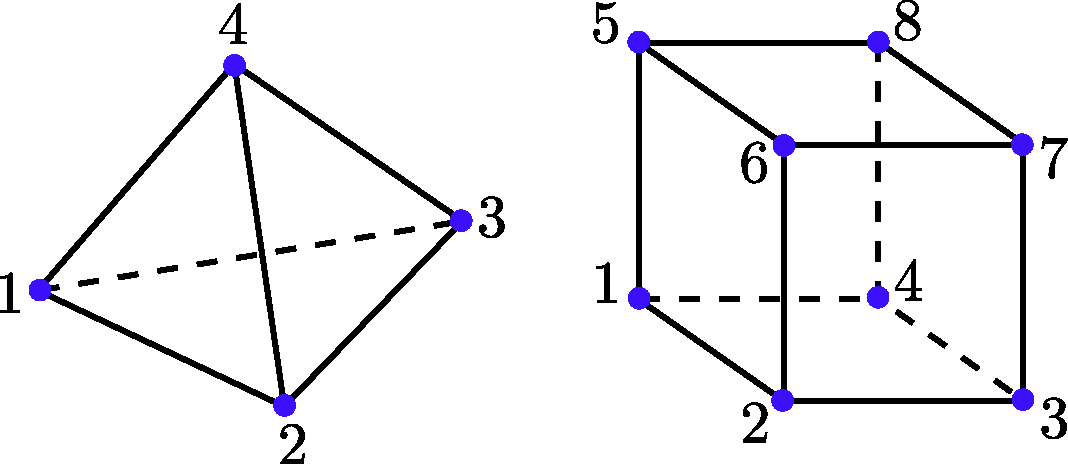
\includegraphics[width = 4.0in]{figures/canonical_orderings.pdf}
		\caption{Canonical node numbering schemes for a linear tetrahedral element (left) and a linear hexahedral element (right). Each of these standard orderings induce corresponding nodal orderings for each triangular or quadrilateral face of the element, as well.}
		\label{fig:canonical_orderings}
	\end{figure}
	
	Polytopal elements with arbitrary topology (with a variable number of nodes, edges, and faces) cannot be represented in this fashion. As a consequence, more descriptive data structures are necessary to fully determine a polytopal element's nodal connectivity. A particular scheme to represent an arbitrary polyhedron within a finite element mesh is described in the following section.

\subsection*{Geometric Data Structures for Arbitrary Polytopes}

	There are multiple ways in which the geometry of a given polyhedral element $\Omega$ may be represented within a finite element code. Ideally, however, the chosen data structure should be made as compact as possible, for the sake of minimizing the storage requirements of a single element. This section describes a few basic data structures for storing arbitrary polygonal and polyhedral shapes within an unstructured finite element mesh.
	
	The geometric data used to describe a typical finite element mesh consists of the following:
	\begin{itemize}
		\item A list of the spatial coordinates $\left\{ \bm{X}_a \right\}_{a=1}^{N^{\mathcal{B}_0}_V}$ for all nodes in the mesh. The sub-index $a \in 1, \ldots, N^{\mathcal{B}_0}_V$ induces a \textit{global node ID} ascribed to each node.
		\item A list of all elements $\left\{ \Omega_{e} \right\}_{e = 1}^{N^{\mathcal{B}_0}_\Omega}$ where $\Omega_{e} \subset \mathcal{B}_0$. The sub-index $e \in 1, \ldots, N^{\mathcal{B}_0}_\Omega$ induces an associated \textit{element ID}.
		\item A list of all faces $\left\{ F_{b} \right\}_{b = 1}^{N^{\Gamma^{\mathrm N}_0}_F}$ where $F_{b} \subset \Gamma^{\mathrm N}_0$ to which traction boundary conditions are assigned. Likewise, the sub-index $b \in 1, \ldots, N^{\Gamma^{\mathrm N}_0}_F$ induces a \textit{boundary face ID}.
	\end{itemize}
	
	In a finite element mesh consisting of arbitrary polyhedral elements, it is suggested that each element $\Omega_e$ be represented by the following data:
	\begin{itemize}
		\item A list of the global node IDs $\left\{ a_i \right\}_{i=1}^{N^{\Omega_e}_V}$ comprising the set of nodes belonging to $\Omega_e$. The sub-index $i \in 1, \ldots, N^{\Omega_e}_V$ induces a \textit{local node ID}, particular to the element $\Omega_e$.
		\item A list of the polygonal faces $\left\{ F_{j} \right\}_{j=1}^{N^{\Omega_e}_F}$ which belong to $\partial \Omega_e$; each polygonal face $F_j$ is in turn represented by a cycle of local node IDs denoted $\left\{ n_i \right\}_{i=1}^{N^{F_j}_V}$, which further determine each face's outward orientation with respect to the element $\Omega_e$.
	\end{itemize}
	An illustration of this collection of data for a given polyhedron $\Omega_e$ is provided in Figure \ref{fig:polyhedron_data}.
	\begin{figure} [!ht]
		\centering
		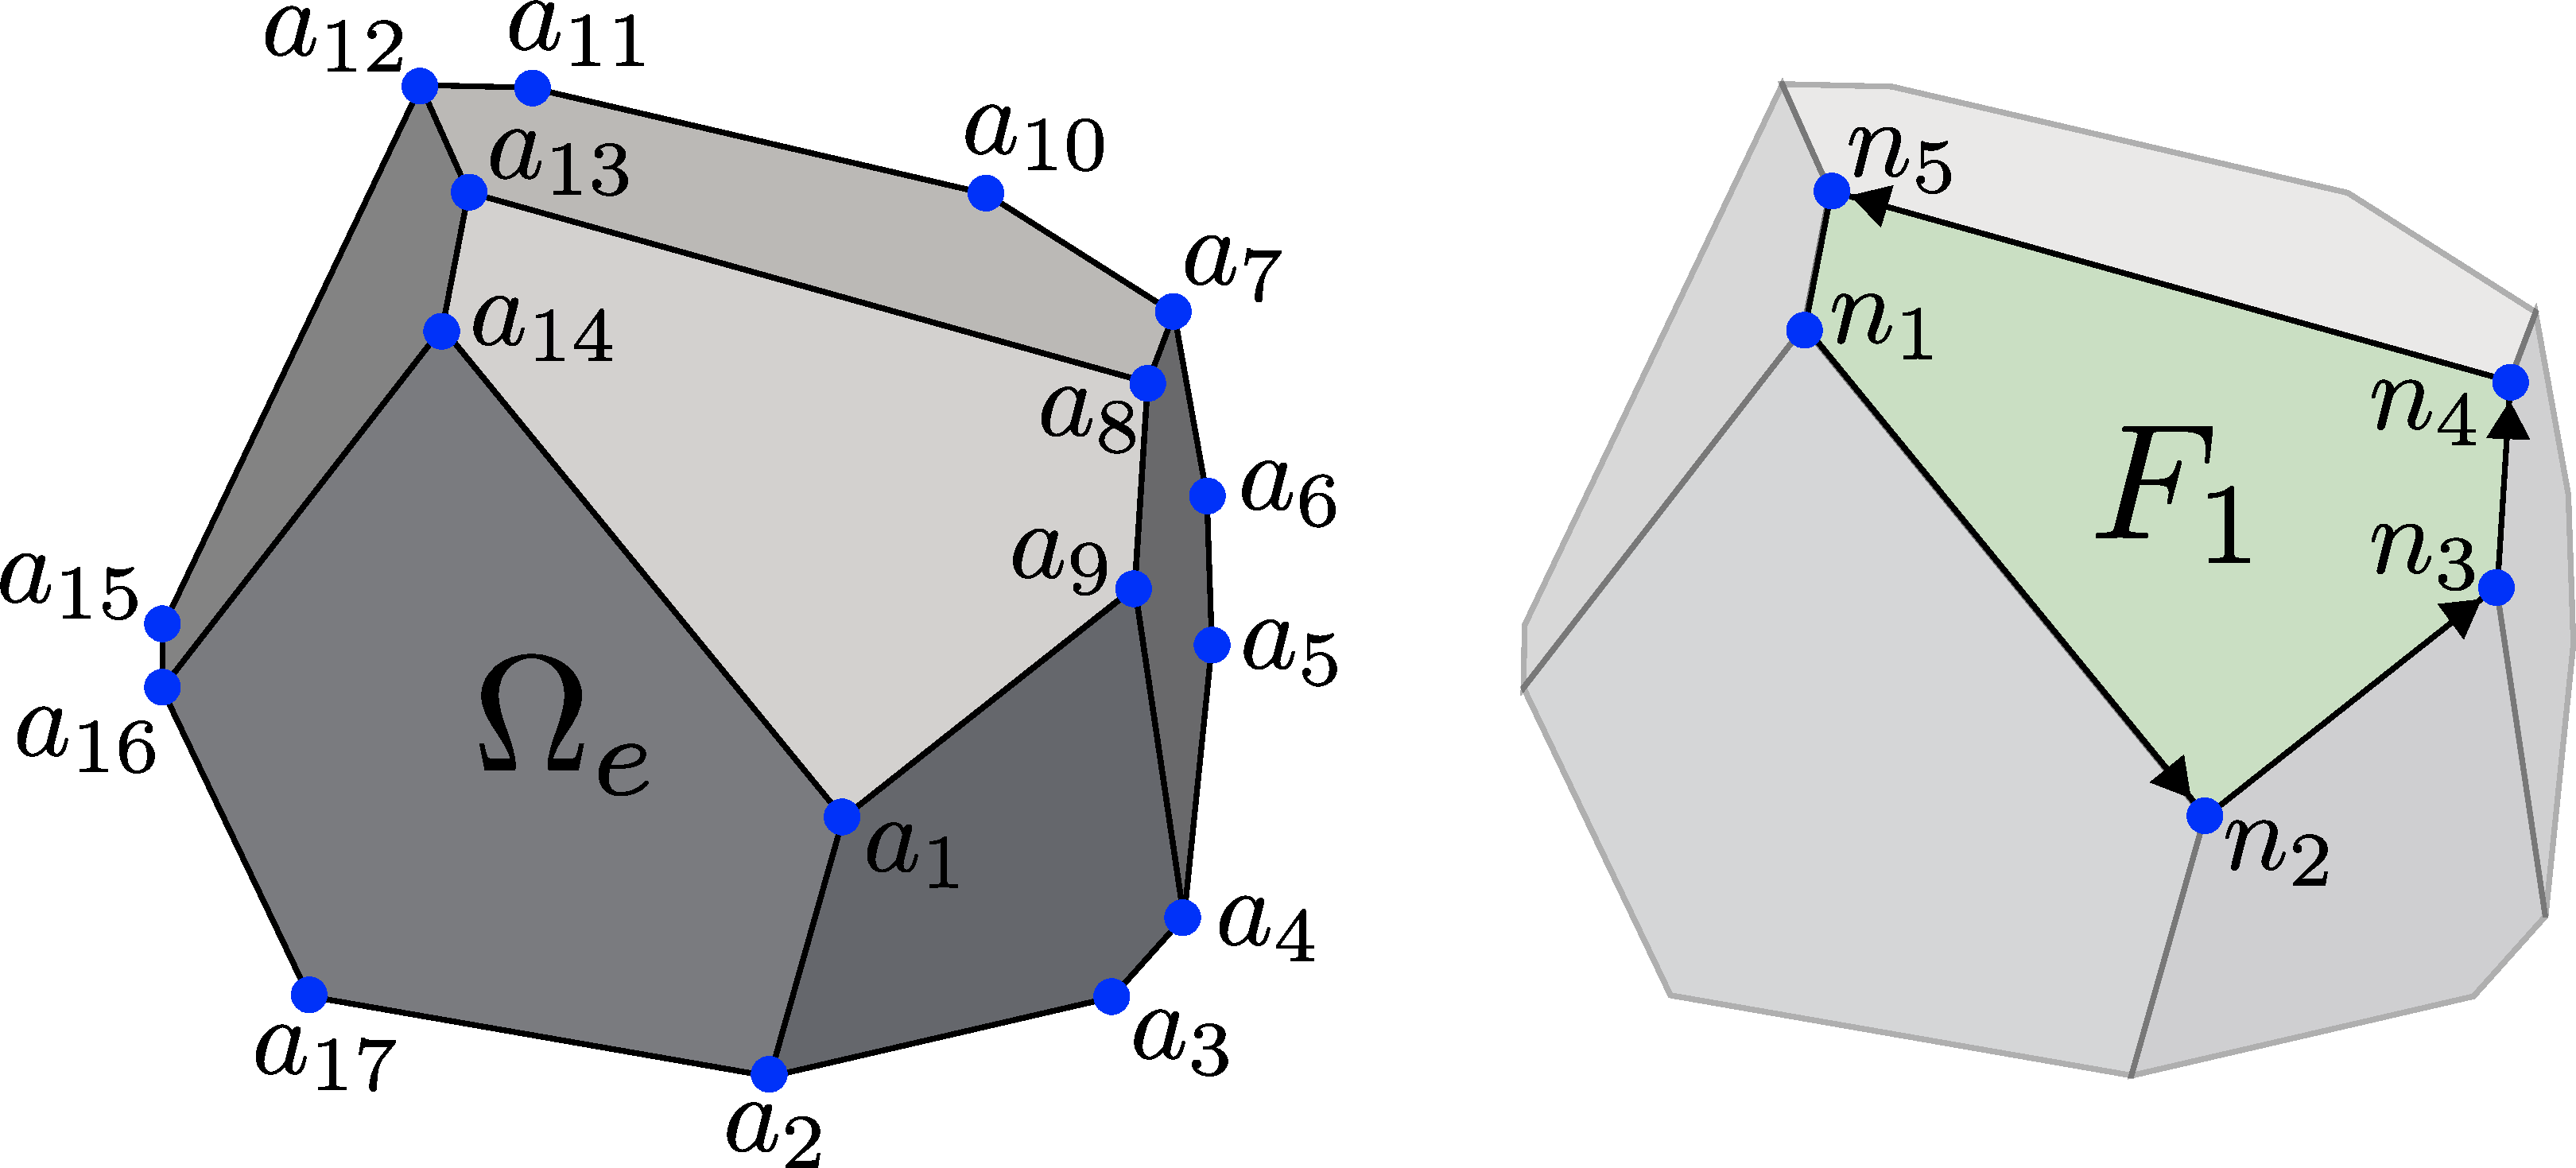
\includegraphics[width = 6.0in]{figures/polyhedron_data.pdf}
		\caption{Illustration of the data necessary to describe an arbitrary polyhedral element $\Omega_e$. The local node ID ordering for the face $F_1$ shown would be $\left\{ n_i \right\}_{i=1}^{5} = \left\{ 14, \, 1, \, 9, \, 8, \, 13 \right\}$.}
		\label{fig:polyhedron_data}
	\end{figure}
	
	A given polygonal face $F_b \subset \Gamma^{\mathrm N}_0$ will similarly be represented by:
	\begin{itemize}
		\item A list of the global node IDs $\left\{ a_i \right\}_{i=1}^{N^{F_b}_V}$ which belong to $F_b$.
		\item A list of the linear edges $\left\{ E_{c} \right\}_{c=1}^{N^{F_b}_E}$ which belong to $\partial F_b$; each linear edge $E_c$ is in turn represented as an ordered list of local node IDs $\left\{ n_i \right\}_{i=1}^{N^{E_c}_V}$.
	\end{itemize}
	
	Unlike canonical finite element shapes, the ordering of the element's nodal IDs is effectively arbitrary, and does not induce a topology. Rather, the element's topology is determined by virtue of its polygonal faces, and their respective (conventionally counter-clockwise) local node orderings. Consequently, each edge of a given polyhedron is defined implicitly as the intersection of two adjacent faces' ordered node sets. Such a scheme may be easily generalized to accommodate serendipity elements containing additional nodes along element edges, as illustrated in Figure \ref{fig:polyhedron_data_quadratic}.
	\begin{figure} [!ht]
		\centering
		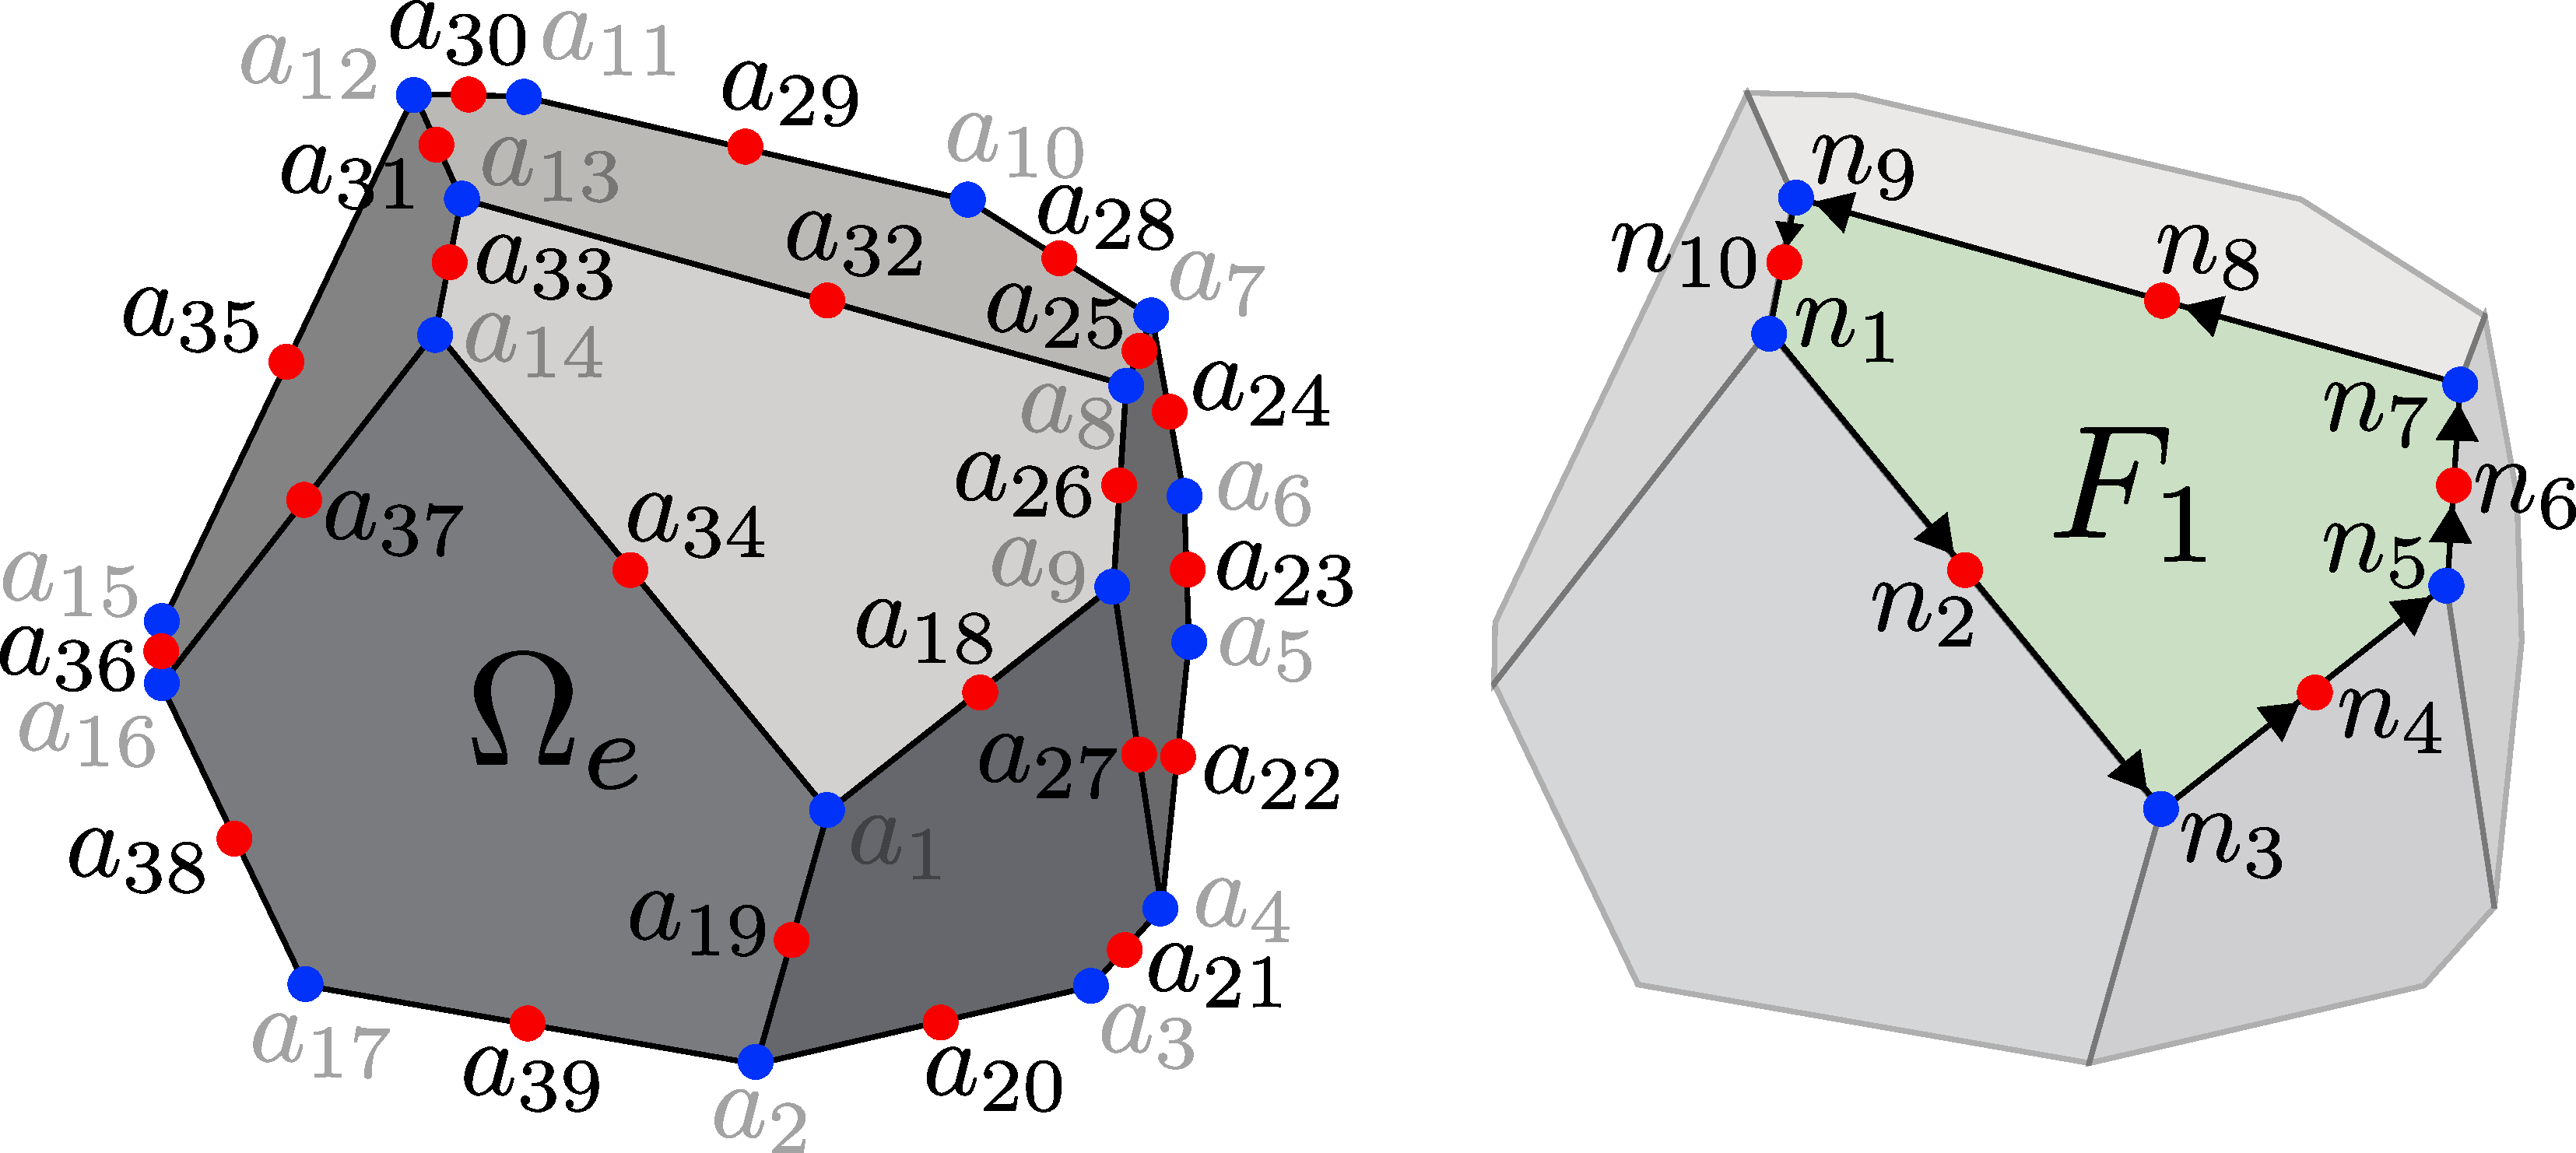
\includegraphics[width = 6.0in]{figures/polyhedron_data_quadratic.pdf}
		\caption{Illustration of the data necessary to describe a quadratic serendipity polyhedral element $\Omega_e$. The local node ID ordering for the face $F_1$ shown would be $\left\{ n_i \right\}_{i=1}^{10} = \left\{ 14, \, 34, \, 1, \, 18, \, 9, \, 26, \, 8, \, 32, \, 13, \, 33 \right\}$.}
		\label{fig:polyhedron_data_quadratic}
	\end{figure}
	
\subsection*{Finite Element Data for Arbitrary Polytopes}

	Traditional Lagrangian finite element methods require each element $\Omega_e \subset \mathcal{B}_0$ to carry the following data (at a minimum) for the purposes of evaluating weak form integrals:
	\begin{itemize}
		\item A list of quadrature weights and corresponding locations $\left\{ w_q, \, \bm{X}_q \right\}_{q=1}^{N^{\Omega_e}_{\mathrm q\mathrm p}}$ associated with the quadrature points of the element. The sub-index $q$ induces a local \textit{quadrature point ID}.
		\item Evaluations of the element's nodal shape functions $\left\{ \varphi_a (\bm{X}_q) \right\}_{q=1}^{N^{\Omega_e}_{\mathrm q\mathrm p}} \, \, \forall a = 1, \ldots, N^{\Omega_e}_V$ at each quadrature point location $\bm{X}_q$.
		\item Gradients (with respect to the element's reference coordinates $\bm{X}$ at time $t = 0$) of the element's nodal shape functions $\left\{ \nabla_X \varphi_a (\bm{X}_q) \right\}_{q=1}^{N^{\Omega_e}_{\mathrm q\mathrm p}} \, \, \forall a = 1, \ldots, N^{\Omega_e}_V$.
		\item (Optionally) if the element relies upon some form of gradient correction scheme (or more generally, if a Petrov-Galerkin method is employed): evaluations and/or gradients of the element's test functions $\left\{ \phi_a (\bm{X}_q), \, \nabla_X \phi_a (\bm{X}_q) \right\}_{q=1}^{N^{\Omega_e}_{\mathrm q\mathrm p}} \, \, \forall a = 1, \ldots, N^{\Omega_e}_V$ must be stored, as well.
	\end{itemize}
	For solid mechanics applications, material state data (e.g. material properties, internal variables, Cauchy stress) would also need to be stored at each quadrature point location.
	
	Similarly, each boundary face $F_b \subset \Gamma^{\mathrm N}_0$ must carry:
	\begin{itemize}
		\item A list of quadrature weights $\left\{ w_q \right\}_{q=1}^{N^{F_b}_{\mathrm q\mathrm p}}$ for each quadrature point of the face.
		\item Evaluations of the face's nodal shape functions $\left\{ \varphi_a (\bm{X}_q) \right\}_{q=1}^{N^{F_b}_{\mathrm q\mathrm p}} \, \, \forall a = 1, \ldots, N^{F_b}_V$ at each quadrature point location $\bm{X}_q$.
		\item Gradients (with respect to the face's in-plane reference coordinates $\bm{X}$ at $t = 0$) of the face's nodal shape functions $\left\{ \nabla_X \varphi_a (\bm{X}_q) \right\}_{q=1}^{N^{F_b}_{\mathrm q\mathrm p}} \, \, \forall a = 1, \ldots, N^{F_b}_V$.
		\item If a Petrov-Galerkin method is employed: evaluations of the face's test functions $\left\{ \phi_a (\bm{X}_q) \right\}_{q=1}^{N^{F_b}_{\mathrm q\mathrm p}} \, \, \forall a = 1, \ldots, N^{F_b}_V$.
		\item Outward unit normals $\left\{ \bm{N}_q \right\}_{q=1}^{N^{F_b}_{\mathrm q\mathrm p}}$ to the face $F_b$ at each quadrature point.
	\end{itemize}
	
	The data enumerated above must be determined via a specified \textit{element formulation}: the method by which the element's shape functions and quadrature rule are constructed. Partitioned element methods address precisely this task. Given an abstract representation for the geometry of a given polyhedral element $\Omega$ (as discussed in the previous section), a PEM formulation proceeds in a number of distinct steps:
	\begin{itemize}
		\item[1.)] The element (and its faces, edges) are appropriately partitioned into cells (facets, segments, vertices).
		\item[2a.)] Individual nodal shape functions are constructed along each edge $E$ of the element.
		\item[2b.)] Individual nodal shape functions are constructed on each face $F$ of the element.
		\item[2c.)] Individual nodal shape functions are constructed on the interior of the element $\Omega$.
		\item[3.)] The discrete finite element data (including quadrature point evaluations of the shape functions and their gradients) are computed and stored by the element.
		\item[4.)] Any auxiliary data (regarding the element's partitioned geometry, etc.) is discarded.
	\end{itemize}
	
	Depending on how the chosen PEM is carried out, the above process can amount to a relatively large computational expense. However, if a total Lagrangian approach is employed within the associated finite element analysis, then the above methodology would only need to be carried out once for each element, at the beginning of the simulation (prior to the first time step). Consequently, the cost of constructing element shape functions in this manner is amortized over the duration of the analysis.
	
	The subsequent sections of this chapter are dedicated to a more detailed discussion of the aforementioned steps taken to construct a given element's partition, and its shape functions.
	
\section{Element Partitioning Schemes}

	The process of obtaining a suitable partition for a given element constitutes the greatest challenge facing partitioned element methods -- an issue of computational geometry, primarily. A secondary complication arises from the conditions of stability that the element must satisfy: the shape function approximations, and the corresponding quadrature rules defined on the element's partition, must guarantee a sufficiently stable integration of the weak form. For relatively simple shapes, a number of stable partitioning schemes exist. However, for arbitrary shapes, it becomes difficult -- if not impossible -- for a heuristically-driven discretization scheme to guarantee that the resulting partition will satisfy the aforementioned stability requirements.

	For this reason, we will limit our subsequent discussion to \textit{star-convex} element geometries. For such shapes, a relatively simple partitioning scheme is suggested, resembling the decomposition used in the edge-based smoothed finite element method \cite{Liu:09}. Even in the presence of nearly-degenerate features, the resulting partition has been verified to provide sufficiently stable shape function approximations and quadrature rules.

\subsection*{Edge-Based Partitioning for Star-Convex Elements}

	A star-convex shape $\Omega$ is one for which there exists some interior point $\bm{X}^{\Omega}_0 \in \Omega$ such that the line segment connecting any point $\bm{X} \in \Omega$ to $\bm{X}^{\Omega}_0$ is entirely contained within $\Omega$. If $\Omega \subset \mathbb{R}^3$ refers to a polyhedron which is star-convex, this further implies that each polygonal face $F \subset \partial \Omega$ is also star-convex with respect to some point $\bm{X}^{F}_0 \in F$. Any linear edge $E \subset \partial F$ is star-convex with respect to any point $\bm{X} \in E$.
	
	A simple and efficient partitioning scheme is described for polyhedral elements $\Omega$ (and their polygonal faces $F_j$) which are star-convex with respect to their vertex-averaged centroids $\bar{\bm{X}}^{\Omega}_0$ (or $\bar{\bm{X}}^{F_j}_0$), i.e.
	\begin{equation}
		\bar{\bm{X}}^{\Omega}_0 = \frac{1}{N^{\Omega}_V} \sum_{i = 1}^{N^{\Omega}_V} \bm{X}_{i}, \quad \text{and} \quad \bar{\bm{X}}^{F_j}_0 = \frac{1}{N^{F_j}_V} \sum_{i = 1}^{N^{F_j}_V} \bm{X}_{i}.
	\end{equation}
	
	For a given polyhedral element $\Omega$, the algorithm proceeds in several steps:
	\begin{itemize}
		\item[1.)] Identify all edges of the polyhedron, and subdivide them into linear segments; each segment should join two adjacent nodes of a given edge.
		\item[2.)] For each face, compute its vertex-averaged centroid $\bar{\bm{X}}^{F_j}_0$, and subdivide the face into triangular facets which emanate from $\bar{\bm{X}}^{F_j}_0$; each facet should share at most two segments (at least one segment) with $\partial F_j$.
		\item[3a.)] Compute the element's vertex-averaged centroid $\bar{\bm{X}}^{\Omega}_0$, and subdivide the element into tetrahedra which emanate from $\bar{\bm{X}}^{\Omega}_0$; each tetrahedron should share a single facet with $\partial \Omega$.
		\item[3b.)] Lump into cells any tetrahedra that share a segment belonging to an edge of $\Omega$; each cell should consist of exactly two tetrahedra.
	\end{itemize}
	An illustration of this process is depicted in Figure \ref{fig:partitioning_algorithm}. A similar algorithm may be applied to each boundary face $F_b \subset \Gamma^{\mathrm N}_0$, entailing only the first two steps described above.
	\begin{figure} [!ht]
		\centering
		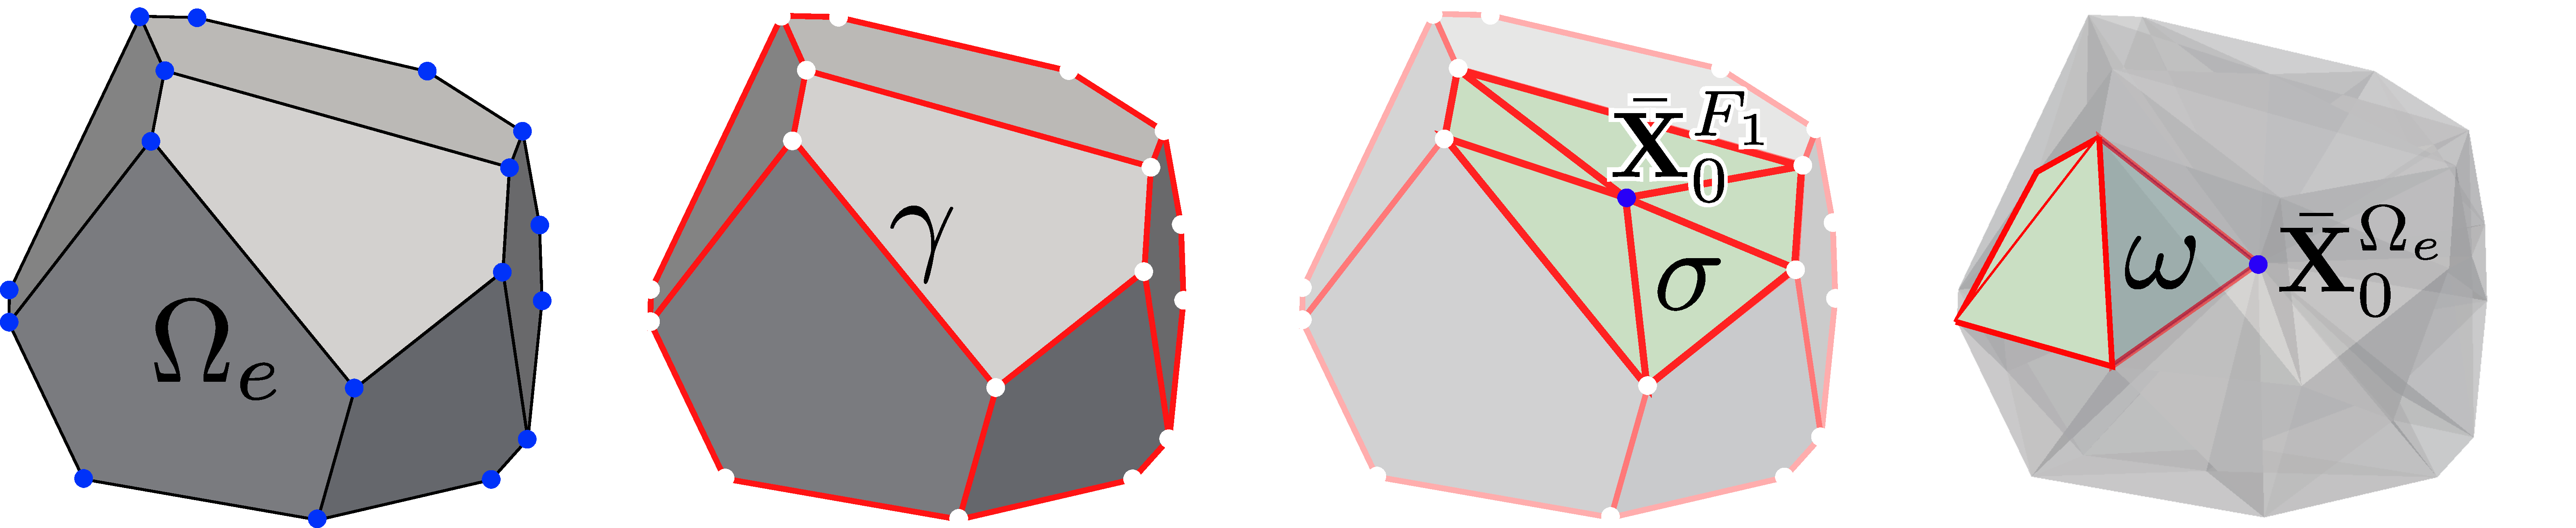
\includegraphics[width = 6.0in]{figures/partitioning_algorithm.pdf}
		\caption{The resulting segment, facet, and cell decomposition for the proposed edge-based partitioning algorithm.}
		\label{fig:partitioning_algorithm}
	\end{figure}
	
	The algorithm can also be naturally extended to accommodate serendipity polyhedral elements, with additional nodes belonging to element edges, as depicted in Figure \ref{fig:partitioning_algorithm_quadratic}.
	\begin{figure} [!ht]
		\centering
		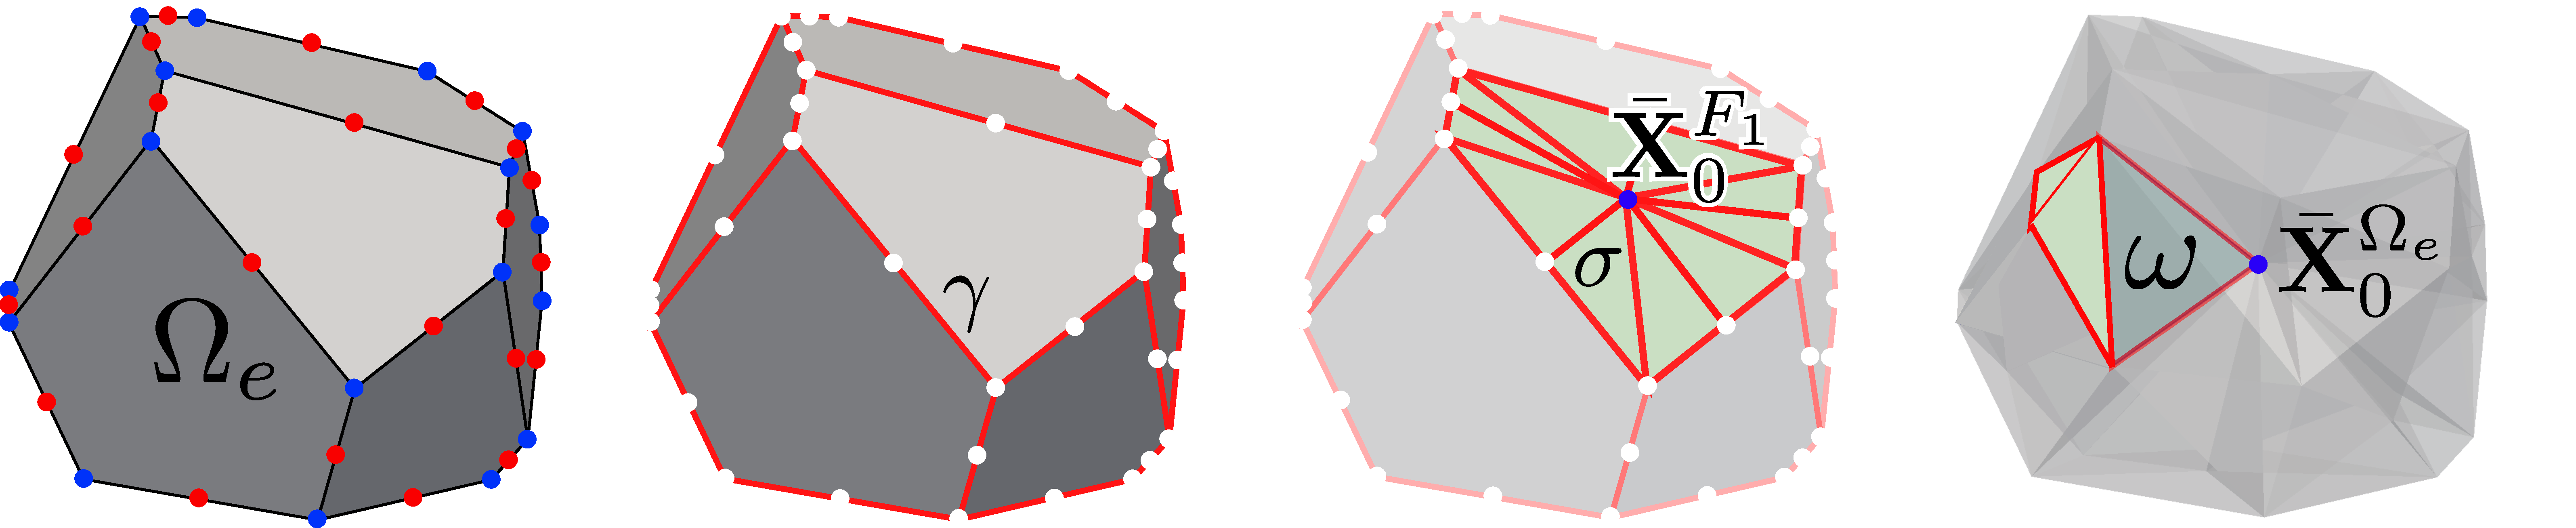
\includegraphics[width = 6.0in]{figures/partitioning_algorithm_quadratic.pdf}
		\caption{The resulting segment, facet, and cell decomposition for the proposed edge-based partitioning algorithm, applied to a quadratic serendipity polyhedral element.}
		\label{fig:partitioning_algorithm_quadratic}
	\end{figure}
	
	A crucial advantage of this approach is that the partition deterministically obtained for each edge (face) will be identical between all elements that share that edge (face), leading to direct satisfaction of (\ref{eq:face_constraint}). As such, the gradient correction schemes discussed in section \ref{sec:quadrature} may be applied independently to each element. Moreover, because each element may be partitioned in an autonomous fashion (without knowledge of any neighboring elements), the computations required to construct each element's shape functions can be directly parallelized.

\section{Abstract Geometric Data Structures}

	Because partitioned element methods consist of solving a set of 1D, 2D, and 3D problems on each edge, face, and element, there arise a number of similarities between these problems of variable dimension. Namely, the geometric data describing each cell, facet, segment and vertex may be abstracted through the use of generic parent-child (tree-based) data structures. Instead of requiring a separate implementation for the solution of each 1D, 2D, 3D problem, generic programming paradigms are exploited to facilitate a single, unified implementation which is agnostic to the dimensionality of the problem being solved. The proposed organization shares many similarities with the generic programming approaches presented in \cite{Cicuttin:17}. A number of definitions for the abstract data structures used henceforth are given in the following sections.
	
\subsection*{Geometric Entities}

	\textit{Geometric entities} (or simply \textit{entities}) are defined as the atomic units of the element's geometric partition. An entity may be: a polyhedral cell, a polygonal facet, a linear segment, or a vertex. Entities are defined in terms of their relationship to other geometric entities. Specifically, a $3-$dimensional entity (a polyhedral cell $\omega$) is uniquely defined in terms of its $2$-dimensional facets $\sigma \subset \partial \omega$ (termed the ``children'' of $\omega$). Each facet $\sigma$ is in turn considered a $2$-dimensional entity, defined in terms of its $1$-dimensional children (its bounding segments $\gamma \subset \partial \sigma$). An entity of dimension $0$ (a vertex) is identified as having no children.
	
	Each geometric entity may be viewed as a ``node'' in a corresponding tree diagram, as illustrated in Figure \ref{fig:entity_tree}, where the height of a given entity within the tree structure indicates its dimensionality $d$.
	\begin{figure} [!ht]
		\centering
		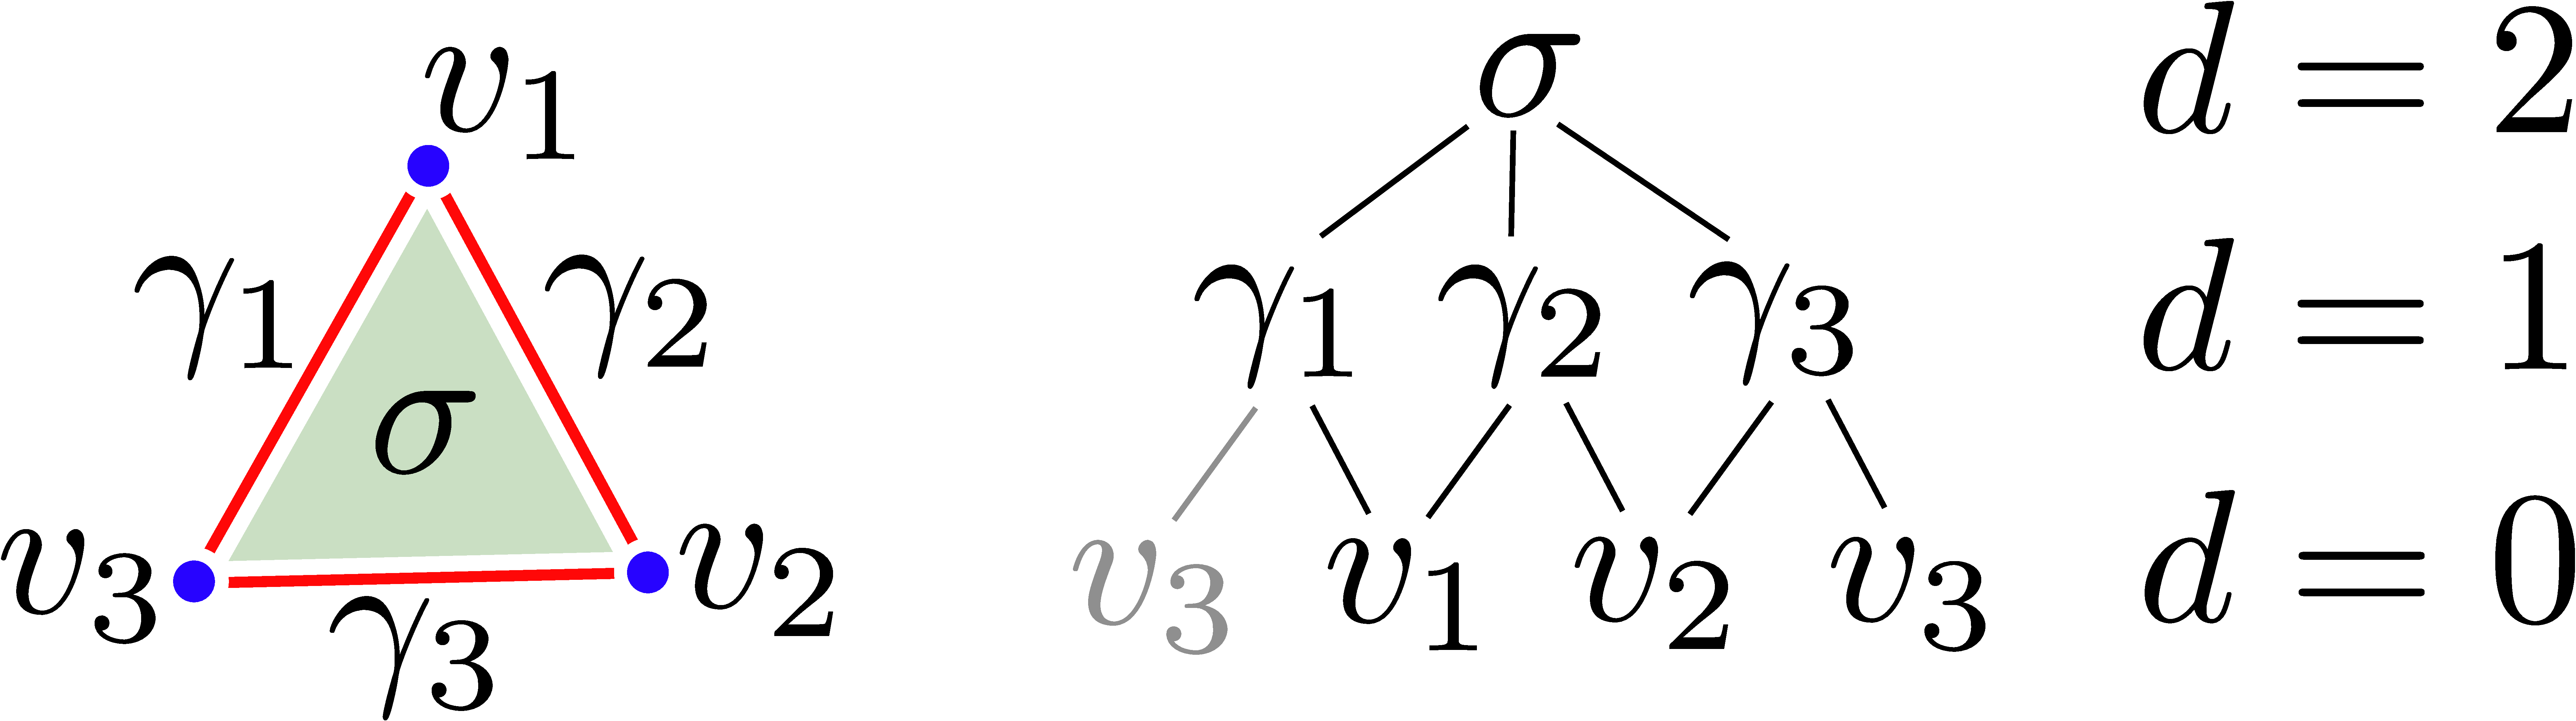
\includegraphics[width = 5.0in]{figures/entity_tree.pdf}
		\caption{A representative entity tree diagram for a $2$-dimensional facet $\sigma$ and its children.}
		\label{fig:entity_tree}
	\end{figure}
	
	Henceforth, we denote by $\varepsilon$ any generic $d-$dimensional entity, and by $\zeta$ any $(d-1)$-dimensional child of $\varepsilon$ (such that $\zeta \subset \partial \varepsilon$). The data stored on a given entity $\varepsilon$ consists of:
	\begin{itemize}
		\item Information (pointers or entity IDs) referring to the $(d-1)$-dimensional children of $\varepsilon$, and/or information (pointers or entity IDs) referring to the $(d+1)$-dimensional parents of $\varepsilon$.
		\item An (optional) orientation/unit direction $\bm{N}_\varepsilon$.
		\item A quadrature rule $\left\{ \bm{X}_q, w_q \right\}_{q=1}^{N^{\varepsilon}_{\mathrm q\mathrm p}}$ defined on $\varepsilon$, or pre-computed monomial integrals $\int_{\varepsilon} \bm{X}^\alpha \, \mathrm d \varepsilon$ for all $|\alpha| \leq k$ (alternatively, the shifted monomials $\int_{\varepsilon} (\bm{X}-\bm{X}_{\varepsilon})^\alpha \, \mathrm d \varepsilon$ may be computed and stored, instead.)
		\item A list of the DG-PEM basis function IDs which possess compact support over $\varepsilon$.
	\end{itemize}
	
	If quadrature rules are to be defined on each geometric entity, we may exploit the particular choice made regarding the element's edge-based partition, noting that every polygonal facet will be a triangle, and every polyhedral cell will consist of two adjoining tetrahedra, allowing for the use of standard Dunavant \cite{Dunavant:85} and Grundmann-M\"{o}ller \cite{Grundmann:78} quadrature rules for triangles and tetrahedra, respectively. Standard Gaussian quadrature rules may be specified on each linear segment.
	
	The advantage of defining entities in this fashion is that it affords greater flexibility in solving the DG-PEM problem (\ref{eq:dg_poisson}) on elements with arbitrary dimensionality.
	
\subsection*{Sub-Elements}

	Herein, a \textit{sub-element} (generically denoted as $\mathcal{E}$) is defined as a $d-$dimensional polytope (a polyhedral element, a polygonal face, a linear edge, or a node) upon which nodal shape functions are locally constructed and defined as the solution to a $d-$dimensional boundary value problem. Sub-elements consist of a partition $\mathcal{T}_{\varepsilon} (\mathcal{E})$ of $\mathcal{E}$ into $d-$dimensional entities $\varepsilon$. The boundary of each sub-element $\mathcal{E}$ is comprised of $(d-1)-$dimensional sub-elements, denoted $e \subset \partial \mathcal{E}$ (called the ``children'' of $\mathcal{E}$, in analog to the terminology used for geometric entities). A sub-element of dimension $0$ (a node) refers to a single vertex, and possesses no children.
	
	As a representative example, consider the face $F \subset \partial \Omega$ shown in Figure \ref{fig:sub_element}, which is classified as a $2-$dimensional sub-element, whose partition $\mathcal{T}_\sigma (F)$ consists of $2-$dimensional facets $\sigma \subset F$. The children of $F$ are comprised of $1-$dimensional sub-elements -- edges $E \subset \partial F$; in turn, the children of each edge $E$ are the nodes of the element. As with geometric entities, the parent-child relationships between different sub-elements induces a tree-like data structure, where the height of a given sub-element within the tree corresponds to its dimensionality $d$.
	\begin{figure} [!ht]
		\centering
		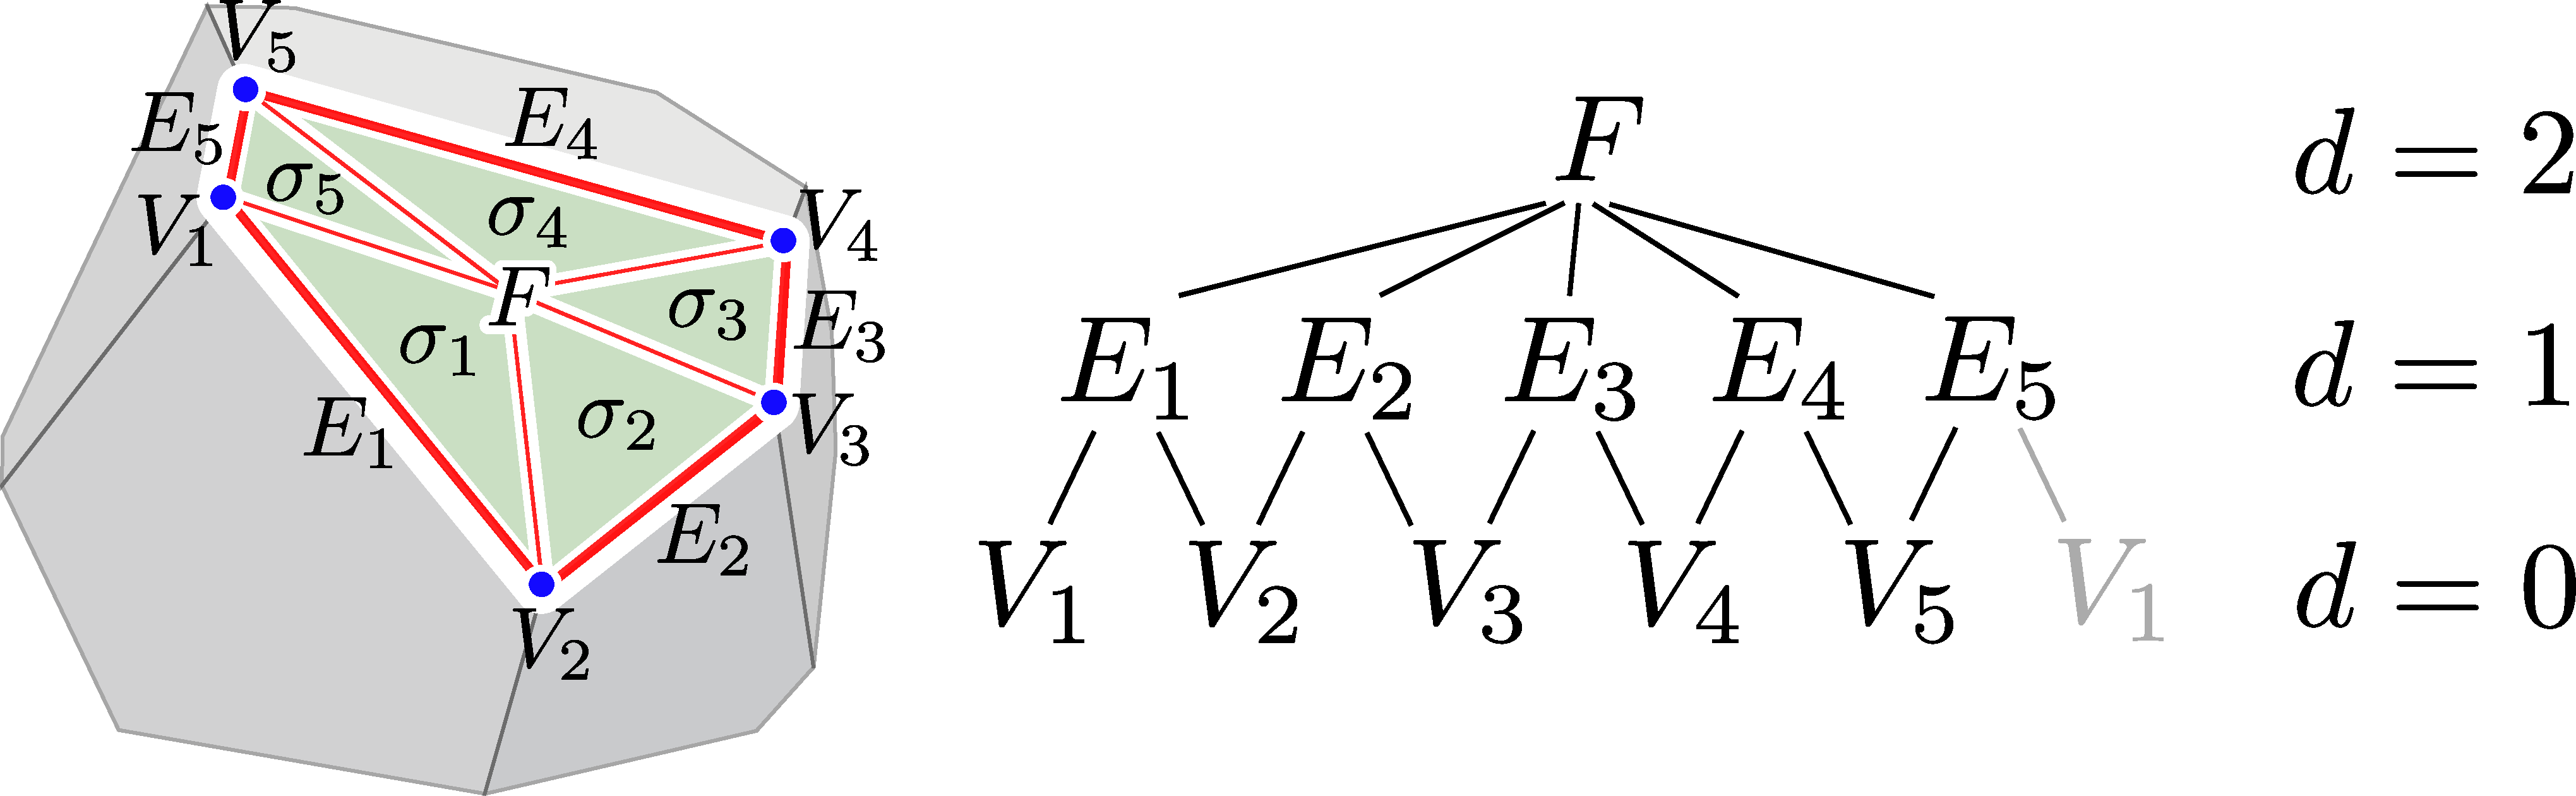
\includegraphics[width = 6.0in]{figures/sub_element.pdf}
		\caption{A representative $2$-dimensional sub-element $F \subset \partial \Omega$ (a polygonal face), and its corresponding sub-element tree diagram. The partition of $F$ consists of polygonal facets $\sigma_i \in \mathcal{T}_{\sigma} (F) \, \, \forall i = 1, \ldots, 5$.}
		\label{fig:sub_element}
	\end{figure}
	
	The data stored for a given sub-element $\mathcal{E}$ consists of:
	\begin{itemize}
		\item Information (pointers or entity IDs) referring to the $d$-dimensional entities $\varepsilon \in \mathcal{T}_\varepsilon (\mathcal{E})$ belonging to the partition of $\mathcal{E}$.
		\item Information (pointers or sub-element IDs) referring to the $(d-1)$-dimensional children of $\mathcal{E}$ (the sub-elements $e \subset \partial \mathcal{E}$ which constitute the boundary of $\mathcal{E}$).
		\item A list of the DG-PEM basis function IDs which are defined on $\mathcal{T}_\varepsilon (\mathcal{E})$.
	\end{itemize}
	
	A more through discussion is dedicated to the subject of DG-PEM basis functions in the following section.
	
\section{Partition-Based Approximation Spaces}

		As discussed in chapter \ref{ch:pem}, partitioned element methods consider a weak formulation of a given PDE (e.g. Laplace's equation), whose solution is approximated through the specification of a finite dimensional function space $\mathcal{U}^h (\mathcal{E})$ defined on the partition $\mathcal{T}_{\varepsilon} (\mathcal{E})$ of a given sub-element $\mathcal{E}$. The (sub-)element's shape functions are selected as the ``best approximations'' to (harmonic) functions which are contained within the chosen approximation space $\mathcal{U}^h (\mathcal{E})$.
		
		Herein, we consider $\mathcal{U}^h (\mathcal{E}) = \mathcal{D}^h_k (\mathcal{E}) = \left\{ \varphi \in L^2 (\mathcal{E}) : \varphi|_{\varepsilon} \in P^k (\varepsilon) \, \forall \varepsilon \in \mathcal{T}_\varepsilon (\mathcal{E}) \right\}$ to be spanned by a set of basis functions $\left\{ \psi_A \right\}_{A=1}^{N^{\mathcal{E}}_{\mathrm b\mathrm f}}$, such that each basis function $\psi \in \mathcal{U}^h (\mathcal{E})$ is compactly supported over a given geometric entity $\varepsilon \in \mathcal{T}_\varepsilon (\mathcal{E})$ (or patch of entities).
		
		Any function $\varphi^h \in \mathcal{U}^h (\mathcal{E})$ may be written as a linear combination of the basis functions which span $\mathcal{U}^h (\mathcal{E})$, i.e.
		\begin{equation}
			\varphi^h (\bm{X}) = \sum_{A=1}^{N^{\mathcal{E}}_{\mathrm b\mathrm f}} \psi_A (\bm{X}) \, \varphi_A \quad \forall \bm{X} \in \mathcal{E}.
		\end{equation}
		The restriction of $\varphi^h$ to a given geometric entity $\varepsilon$ may be written in terms of only those basis functions $\left\{ \psi^\varepsilon_{a} \right\}_{a=1}^{N^\varepsilon_{\mathrm b\mathrm f}} \subset \mathcal{U}^h (\Omega)$ which possess compact support over $\varepsilon$, such that
		\begin{equation}
			\varphi^h|_\varepsilon (\bm{X}) = \sum_{a=1}^{N^\varepsilon_{\mathrm b\mathrm f}} \psi^\varepsilon_{a} (\bm{X}) \, \varphi_{a} \quad \forall \bm{X} \in \varepsilon.
		\end{equation}
		
		To guarantee $P^k (\mathcal{E}) \subset \mathcal{U}^h (\mathcal{E})$ for some desired degree of polynomial completeness $k$, it is necessary for a given entity's local basis $\left\{ \psi^\varepsilon_{a} \right\}_{a=1}^{N^\varepsilon_{\mathrm b\mathrm f}}$ to span $P^k (\varepsilon)$. Arguably the simplest such basis consists of the monomials through order $k$ defined on each entity $\varepsilon \in \mathcal{T}_\varepsilon (\mathcal{E})$. However, the use of (unscaled) monomial bases can lead to ill-conditioning of the DG-PEM problem, particularly as the maximal polynomial degree $k$ is increased. This fact has been well-established in the literature pertaining to discontinuous Galerkin methods (see for example \cite{Hesthaven:10}.) For this reason, other (well-scaled) polynomial bases are recommended, such as the Lagrange polynomials defined on each entity (for linear segments and triangular facets), or the orthogonal polynomials obtained via the methodology proposed in \cite{Bassi:12}. An exploration of the condition number for the resulting DG-PEM systems of equations is presented at the end of this chapter.
		
		Irrespective of the chosen basis, each basis function $\psi (\bm{X})$ may be expressed as a low-order polynomial (of maximal degree $k$) via a linear combination of (possibly shifted) monomials:
		\begin{equation}
			\psi (\bm{X}) = \sum_{|\alpha| \leq k} c_\alpha (\bm{X}-\bm{X}_0)^{\alpha},
		\end{equation}
		where $\alpha = \alpha_1, \ldots, \alpha_d$ is a multi-index, such that $|\alpha| = \alpha_1 + \ldots + \alpha_2$ and $\bm{X}^\alpha = X_1^{\alpha_1} \cdots X_d^{\alpha_d}$. Consequently, a given basis function is uniquely defined in terms of its shifted coordinate $\bm{X}_0$, and its monomial coefficients $c_\alpha$. The gradient of a given basis function $\nabla \psi (\bm{X})$ may in turn be computed via
		\begin{equation}
			\frac{\partial \psi (\bm{X})}{\partial X_i} = \sum_{|\alpha| \leq k} \alpha_i c_\alpha (\bm{X}-\bm{X}_0)^{\alpha_1, \ldots, (\alpha_i - 1), \ldots, \alpha_d}.
		\end{equation}
		
\section{Linearization and Assembly of the DG-PEM Systems of Equations}

	The DG-PEM problem of (\ref{eq:dg_poisson}) may be written in terms of the chosen basis $\left\{ \psi_A \right\}_{A=1}^{N^\mathcal{E}_{\mathrm b\mathrm f}}$ for $\mathcal{D}^h_k (\mathcal{E})$, such that the basis function coefficients $\varphi_A \, \, \forall A = 1, \ldots, N^\mathcal{E}_{\mathrm b\mathrm f}$ representing a given shape function $\varphi^h (\bm{X}) = \sum_{A=1}^{N^\mathcal{E}_{\mathrm b\mathrm f}} \psi_A (\bm{X}) \, \varphi_A$ may be determined as the solution to a linear system of equations:
	\begin{equation}
		\sum_{A=1}^{N^\mathcal{E}_{\mathrm b\mathrm f}} J_{AB} \, \varphi_A = F_B \quad \forall B = 1, \ldots, N^\mathcal{E}_{\mathrm b\mathrm f},
		\label{eq:linearization_dgpem}
	\end{equation}
	where $J_{AB}$ and $F_B$ are computed via an entity-wise assembly process following to the methodology described in \cite{Riviere:08}. In addition to assembling local contributions $J^\varepsilon_{ab}$ and $F^\varepsilon_b$ to $J_{AB}$ and $F_B$ from all $d$-dimensional entities $\varepsilon \in \mathcal{T}_\varepsilon (\mathcal{E})$, it is also necessary to assemble appropriate contributions from all $(d-1)$-dimensional interfaces $\zeta \in \Gamma_\varepsilon \cup \partial \mathcal{E}$, as well.

	Specifically, each $d$-dimensional entity $\varepsilon \in \mathcal{T}_\varepsilon (\mathcal{E})$ contributes the following local arrays:
	\begin{equation}
			J^{\varepsilon}_{ab} = \int_{\varepsilon} \nabla \psi^{\varepsilon}_{a} \, \cdot \nabla \psi^{\varepsilon}_{b} \, \mathrm d \varepsilon, \quad \forall a, \, b = 1, \ldots, N^{\varepsilon}_{\mathrm b\mathrm f},
	\end{equation}
	\begin{equation}
			F^{\varepsilon}_b = \int_{\varepsilon} f_{\mathcal{E}} \, \psi_b^{\varepsilon} \, \mathrm d \varepsilon \quad \forall b = 1, \ldots, N^{\varepsilon}_{\mathrm b\mathrm f}.
	\end{equation}
	Each $\zeta \in \partial \mathcal{E}$ (which borders a single $d$-dimensional entity $\varepsilon$) contributes:
	\begin{equation}
			J^{\varepsilon}_{ab} = \int_{\zeta} \bigg( \epsilon \, (\bm{N}_{\zeta} \cdot \nabla \psi^{\varepsilon}_b) \, \psi^{\varepsilon}_a - \psi^{\varepsilon}_b \, (\bm{N}_{\zeta} \cdot \nabla \psi^{\varepsilon}_a) \bigg) \, \mathrm d \zeta + \frac{\alpha_{\zeta0}}{|\zeta|^{\beta_0}} \int_{\zeta} \psi_a^{\varepsilon} \, \psi_b^{\varepsilon} \, \mathrm d \zeta \quad \forall a, \, b = 1, \ldots, N^{\varepsilon}_{\mathrm b\mathrm f},
	\end{equation}
	\begin{equation}
		F^{\varepsilon}_b = \int_{\zeta} \epsilon \, (\bm{N}_{\zeta} \cdot \nabla \psi_b^{\varepsilon}) \, \bar{\varphi} \, \mathrm d \zeta + \frac{\alpha_{\zeta0}}{|\zeta|^{\beta_0}} \int_{\zeta} \bar{\varphi} \, \psi_b^{\varepsilon} \, \mathrm d \zeta \quad \forall b = 1, \ldots, N^{\varepsilon}_{\mathrm b\mathrm f},
		\label{eq:boundary_term}
	\end{equation}
	and each $\zeta \in \Gamma_\varepsilon$ (which borders two $d$-dimensional entities, $\varepsilon_1$ and $\varepsilon_2$) contributes:
	\begin{align}
			J^{\varepsilon_i \varepsilon_j}_{ab} & = - \frac{1}{2} \int_{\zeta} \bigg( (-1)^{i} \, \epsilon \, (\bm{N}_{\zeta} \cdot \nabla \psi_b^{\varepsilon_j}) \, \psi_a^{\varepsilon_i} - (-1)^{j} \, \psi_b^{\varepsilon_j} (\bm{N}_{\zeta} \cdot \nabla \psi_a^{\varepsilon_i}) \bigg) \, \mathrm d \zeta \\
			& + (-1)^{(i+j)} \frac{\alpha_{\zeta0}}{|\zeta|^{\beta_0}} \int_{\zeta} \psi_a^{\varepsilon_i} \, \psi_b^{\varepsilon_j} \, \mathrm d \zeta \\
			& + (-1)^{(i+j)} \frac{\alpha_{\zeta1}}{|\zeta|^{\beta_1}} \int_{\zeta} \nabla \psi_a^{\varepsilon_i} \cdot (\bm{N}_\zeta \otimes \bm{N}_\zeta) \cdot \nabla \psi_b^{\varepsilon_j} \, \mathrm d \zeta
	\end{align}
	for all $i, \, j = 1, \, 2$, and $a = 1, \ldots, N^{\varepsilon_i}_{\mathrm b\mathrm f}$, $b = 1, \ldots, N^{\varepsilon_j}_{\mathrm b\mathrm f}$. For the remainder of our discussions, we will consider only the case where $f_\mathcal{E} \equiv 0$ for all sub-elements $\mathcal{E} \subset \Omega$.
	
	For a given $d$-dimensional sub-element $\mathcal{E}$, the assembly of the above terms entails an entity-wise integration of products between basis functions (and their gradients) over $d$-dimensional entities $\varepsilon \in \mathcal{T}_\varepsilon (\mathcal{E})$ and their $(d-1)$-dimensional children $\zeta \in \Gamma_\varepsilon \cup \partial \mathcal{E}$. This may be effected through the use of appropriately defined quadrature rules on each entity, or by pre-computing the monomial integrals over each entity up to some sufficiently high degree (nominally $2k$).
	
	Additionally, it is remarked that the boundary condition $\bar{\varphi}$ is defined independently on every $(d-1)$-dimensional sub-element $e \subset \partial \mathcal{E}$, such that its restriction $\bar{\varphi}|_\zeta$ may be written in terms of the local basis functions $\left\{ \psi^{\zeta}_c \right\}_{c=1}^{N^\zeta_{\mathrm b\mathrm f}}$ belonging to a given boundary entity $\zeta \in \mathcal{T}_{\zeta} (e)$, i.e.
	\begin{equation}
			\bar{\varphi}|_\zeta (\bm{X}) = \sum_{c=1}^{N^\zeta_{\mathrm b\mathrm f}} \psi^\zeta_c (\bm{X}) \, \bar{\varphi}_c.
	\end{equation}
	For a given $\zeta \in \partial \mathcal{E}$, this yields:
	\begin{equation}
		F^{\varepsilon}_b = \sum_{c=1}^{N^\zeta_{\mathrm b\mathrm f}} \bar{J}^{\varepsilon}_{bc} \, \bar{\varphi}_c \quad \forall b = 1, \ldots, N^{\varepsilon}_{\mathrm b\mathrm f},
	\end{equation}
	which may be used in lieu of (\ref{eq:boundary_term}), where
	\begin{equation}
		\bar{J}^{\varepsilon}_{bc} = \int_{\zeta} \epsilon \, (\bm{N}_{\zeta} \cdot \nabla \psi_b^{\varepsilon}) \, \psi^\zeta_c  \, \mathrm d \zeta + \frac{\alpha_{\zeta0}}{|\zeta|^{\beta_0}} \int_{\zeta} \psi^\zeta_c \, \psi_b^{\varepsilon} \, \mathrm d \zeta \quad \forall b = 1, \ldots, N^{\varepsilon}_{\mathrm b\mathrm f}, \, c = 1, \ldots, N^\zeta_{\mathrm b\mathrm f}.
	\end{equation}
	Consequently, we may re-write the right-hand side of (\ref{eq:linearization_dgpem}) as a linear mapping from the basis coefficients $\bar{\varphi}_C$ which determine the boundary function $\bar{\varphi} (\bm{X}) = \sum_{C=1}^{N^{\partial \mathcal{E}}_{\mathrm b\mathrm f}} \psi_C (\bm{X}) \, \bar{\varphi}_C$:
	\begin{equation}
		\sum_{A=1}^{N^{\mathcal{E}}_{\mathrm b\mathrm f}} J_{AB} \, \varphi_A = \sum_{C=1}^{N^{\partial \mathcal{E}}_{\mathrm b\mathrm f}} \bar{J}_{BC} \, \bar{\varphi}_C \quad \forall B = 1, \ldots, N^{\mathcal{E}}_{\mathrm b\mathrm f}.
	\end{equation}
	Alternatively, in matrix-vector format:
	\begin{equation}
		\bm{J} \, \boldsymbol{\varphi} = \bar{\bm{J}} \, \bar{\boldsymbol{\varphi}}.
		\label{eq:dgpem_linear_system}
	\end{equation}
	
	The above system of equations can be solved to obtain a linear mapping from $\bar{\boldsymbol{\varphi}}$ to $\boldsymbol{\varphi}$, denoted $\bm{M}^{\partial \mathcal{E} \mapsto \mathcal{E}} = \bm{J}^{-1} \bar{\bm{J}} : \mathbb{R}^{N^{\partial \mathcal{E}}_{\mathrm b\mathrm f}} \mapsto \mathbb{R}^{N^{\mathcal{E}}_{\mathrm b\mathrm f}}$. This mapping may be utilized to define the shape functions in a recursive fashion (over the children of each sub-element, in succession), ultimately yielding a representation for the shape functions on $\mathcal{E}$ in terms of only nodal evaluations $\varphi|_{V}$. This process is discussed in greater detail in the following section.
	
\subsection*{Hierarchical Construction of Shape Functions}

	For a given polyhedral element $\Omega \subset \mathbb{R}^d$, we presume that each shape function $\varphi_A$ is associated with a particular node $V_A$ of the element, such that
	\begin{equation}
		\varphi_A |_{V_B} = \delta_{AB} \quad \forall A, \, B = 1, \ldots, N^{\Omega}_V.
	\end{equation}
	
	Additionally, for the sake of simplicity (and computational efficiency), it is suggested that the shape functions along each linear edge $E$ be constructed from the standard Lagrange polynomials which interpolate the nodal values of that edge.

	For each polygonal face $F$, linear mappings $\bm{M}^{\partial F \mapsto F} : \mathbb{R}^{N^{F}_{V}} \mapsto \mathbb{R}^{N^{F}_{\mathrm b\mathrm f}}$ may be constructed according to the process described in the previous section, yielding 
	\begin{equation}
		\varphi_A |_{F} (\bm{X}) = \sum_{b = 1}^{N^F_{\mathrm b\mathrm f}} \sum_{c = 1}^{N^F_{V}} \psi_b (\bm{X}) \, M^{\partial F \mapsto F}_{bc} \varphi_A |_{V_c}.
	\end{equation}

	Subsequently, a mapping $\bm{M}^{\partial \Omega \mapsto \Omega} : \mathbb{R}^{N^{\partial \Omega}_{\mathrm b\mathrm f}} \mapsto \mathbb{R}^{N^{\Omega}_{\mathrm b\mathrm f}}$ is constructed to determine the representation for the shape functions on the interior of the element, which may be composed with the mappings $\bm{M}^{\partial F \mapsto F}$ for each face to determine a final mapping $\bm{M}^{V \mapsto \Omega} : \mathbb{R}^{N^{\Omega}_{V}} \mapsto \mathbb{R}^{N^{\Omega}_{\mathrm b\mathrm f}}$ which yields
	\begin{equation}
		\varphi_A |_{\Omega} (\bm{X}) = \sum_{b = 1}^{N^\Omega_{\mathrm b\mathrm f}} \sum_{c = 1}^{N^\Omega_{V}} \psi_b (\bm{X}) \, M^{V \mapsto \Omega}_{bc} \varphi_A |_{V_c}.
		\label{eq:mapped_shape_functions}
	\end{equation}

	Once the above representations for the element's shape function have been obtained, the discrete data required of the element (evaluations of the shape functions and their gradients at a discrete number of quadrature points $\left\{ \bm{X}_q \right\}_{q=1}^{N_{\mathrm q\mathrm p}}$) can be obtained through direct evaluation of (\ref{eq:mapped_shape_functions}), i.e.
	\begin{equation}
		\varphi_A |_{\Omega} (\bm{X}_q) = \sum_{b = 1}^{N^\Omega_{\mathrm b\mathrm f}} \sum_{c = 1}^{N^\Omega_{V}} \psi_b (\bm{X}_q) \, M^{V \mapsto \Omega}_{bc} \varphi_A |_{V_c},
	\end{equation}
	and
	\begin{equation}
		\nabla \varphi_A |_{\Omega} (\bm{X}_q) = \sum_{b = 1}^{N^\Omega_{\mathrm b\mathrm f}} \sum_{c = 1}^{N^\Omega_{V}} \nabla \psi_b (\bm{X}_q) \, M^{V \mapsto \Omega}_{bc} \varphi_A |_{V_c}.
	\end{equation}
	Once the discrete quadrature point evaluations for the shape functions have been obtained, there is no need to retain any information regarding the DG-PEM basis functions, or the transitional mappings; these artifacts and their corresponding data structures may therefore be discarded.

	The specification of the element's quadrature rule is discussed in the following section.

\subsection*{Construction of Quadrature Rules}

	The quadrature rule for an element $\left\{ \bm{X}_q, \, w_q \right\}_{q=1}^{N_{\mathrm q\mathrm p}}$ nominally consists of quadrature points $\bm{X}_q$ located at the centroids of each cell $\omega \in \mathcal{T}_\omega (\Omega)$, whose corresponding quadrature weights $w_q$ are equal to the volumes of each respective cell $|\omega|$. This results in the composite mid-point rule discussed in chapter \ref{ch:pem}.

	As previously discussed, the volumes $|\omega|$ and centroids $\bar{\bm{X}}_\omega$ of each cell may be obtained via the exact integration formulas provided by Chin et al. in \cite{Chin:15}. Alternatively, we may exploit the geometric simplicity of the chosen edge-based partitioning scheme to compute these quantities more easily, by considering the fact that each edge-centered cell $\omega$ consists of two tetrahedral sub-domains (i.e. $T_1 \cup T_2 = \omega$). Volumes and centroids for each tetrahedron can be easily computed using standard formulas, and the resulting quantities of interest may be expressed as
	\begin{equation}
		|\omega| = |T_1| + |T_2|, \quad \bar{\bm{X}}_\omega = \frac{|T_1| \bar{\bm{X}}_{T_1} + |T_2| \bar{\bm{X}}_{T_2}}{|\omega|}.
	\end{equation}

	Straightforward integration rules $\left\{ \bm{X}_q, \, w_q \right\}_{q=1}^{N^F_{\mathrm q\mathrm p}}$ for each face $F \subset \partial \Omega$ are more more easily obtained by considering the corresponding areas $|\sigma|$ and centroids $\bar{\bm{X}}_\sigma$ of each (strictly triangular) facet $\sigma \in \mathcal{T}_{\sigma} (F)$. Outward unit normals $\bm{N}_\sigma$ to each facet may also be readily computed and stored, as needed.

	With these quantities in hand, the element's shape functions (and their gradients) may be evaluated at the quadrature points of the element, as described in the previous section. Subsequently, a consistent integration scheme (as discussed in \ref{ch:pem}) may be constructed from the discrete data stored at the element's quadrature points. If a gradient correction scheme is adopted, the corrected test function gradients $\nabla \phi_A (\bm{X}_q)$ at all quadrature points may be computed and stored, as needed.

\section{Numerical Conditioning of the DG-PEM Systems of Equations}

As a representative example, consider a given sub-element $\mathcal{E} \subset \mathbb{R}^d$ and its corresponding partition into $d-$dimensional entities $\varepsilon \subset \mathcal{T}_\varepsilon (\mathcal{E})$. Recall that the representation of a given shape function $\varphi \in \mathcal{D}^h_k (\mathcal{E})$ is piecewise polynomial in each entity, i.e. $\varphi|_{\varepsilon} \in P^k (\varepsilon)$.

A reasonable estimate for the condition number $\kappa (\bm{J})$ of the SPD matrix $\bm{J}$ appearing in (\ref{eq:dgpem_linear_system}) may be obtained via
\begin{equation}
	 \frac{\max_a |J^{\varepsilon}_{aa}|}{\min_a |J^{\varepsilon}_{aa}|} \leq \kappa (\bm{J}),
\end{equation}
where
\begin{align}
	J^{\varepsilon}_{aa} = & \int_{\varepsilon} \nabla \psi^{\varepsilon}_{a} \, \cdot \nabla \psi^{\varepsilon}_{a} \, \mathrm d \varepsilon + (\epsilon-1) \sum_{\zeta \in \partial \varepsilon \cap \partial \mathcal{E}} \int_{\zeta} \left( \psi^{\varepsilon}_a \right) \left( \bm{N}_{\zeta} \cdot \nabla \psi^{\varepsilon}_a \right) \, \mathrm d \zeta \nonumber \\ 
	+ & \frac{1}{2} (\epsilon-1) \sum_{\zeta \in \partial \varepsilon \cap \Gamma_\varepsilon} \int_{\zeta} \left( \psi^{\varepsilon}_a \right) \left( \bm{N}_{\zeta} \cdot \nabla \psi^{\varepsilon}_a \right) \, \mathrm d \zeta \nonumber \\
	+ & \sum_{\zeta \in \partial \varepsilon} \frac{\alpha_{\zeta0}}{|\zeta|^{\beta_0}} \int_{\zeta} \left( \psi_a^{\varepsilon} \right)^2 \, \mathrm d \zeta + \sum_{\zeta \in \partial \varepsilon \cap \Gamma_\varepsilon} \frac{\alpha_{\zeta1}}{|\zeta|^{\beta_1}} \int_{\zeta} \left( \bm{N}_{\zeta} \cdot \nabla \psi^{\varepsilon}_a \right)^2 \, \mathrm d \zeta.
\end{align}
A brief remark should be made regarding the positivity of $J^\varepsilon_{aa}$, and its relation to the particular choice of DG method (i.e. whether the SIPG, NIPG, or IIPG is chosen). As discussed in \cite{Riviere:08}, the NIPG method with $\epsilon = +1$ will yield strictly positive diagonal entries provided $\alpha_{\zeta0} > 0$, resulting in the coercivity of $\bm{J}$. If the SIPG ($\epsilon = -1$) or IIPG ($\epsilon = 0$) methods are employed, then the penalty parameters must be made sufficiently large enough to guarantee coercivity and stability.

The subsequent discussion examines the case where $\epsilon = +1$, yielding strictly positive diagonal entries:
\begin{equation}
	J^{\varepsilon}_{aa} = \int_{\varepsilon} \nabla \psi^{\varepsilon}_{a} \, \cdot \nabla \psi^{\varepsilon}_{a} \, \mathrm d \varepsilon + \sum_{\zeta \in \partial \varepsilon} \frac{\alpha_{\zeta0}}{|\zeta|^{\beta_0}} \int_{\zeta} \left( \psi_a^{\varepsilon} \right)^2 \, \mathrm d \zeta + \sum_{\zeta \in \partial \varepsilon \cap \Gamma_\varepsilon} \frac{\alpha_{\zeta1}}{|\zeta|^{\beta_1}} \int_{\zeta} \left( \bm{N}_{\zeta} \cdot \nabla \psi^{\varepsilon}_a \right)^2 \, \mathrm d \zeta.
\end{equation}
Let $h_{\varepsilon}$ denote the diameter of $\varepsilon$, such that
\begin{equation}
	h_{\varepsilon} = \sup_{\bm{X}_1, \bm{X}_2 \in \varepsilon} ||\bm{X}_1 - \bm{X}_2||_2.
\end{equation}
Using the following trace inequalities:
\begin{equation}
	\int_{\zeta} \left( \psi_a^{\varepsilon} \right)^2 \, \mathrm d \zeta \leq C h_\varepsilon^{-1/2} \int_{\varepsilon} \left( \psi_a^{\varepsilon} \right)^2 \, \mathrm d \varepsilon \quad \forall \zeta \subset \partial \varepsilon,
\end{equation}
\begin{equation}
	\int_{\zeta} \left( \bm{N}_{\zeta} \cdot \nabla \psi^{\varepsilon}_a \right)^2 \, \mathrm d \zeta \leq C h_\varepsilon^{-1/2} \int_{\varepsilon} \nabla \psi^{\varepsilon}_{a} \, \cdot \nabla \psi^{\varepsilon}_{a} \, \mathrm d \varepsilon \quad \forall \zeta \subset \partial \varepsilon,
\end{equation}
and observing that $|\zeta|^{\beta_0} \leq h_\varepsilon$, $|\zeta|^{\beta_1} \geq h_\varepsilon^{-1}$ if $\beta_0 = (d-1)^{-1}$, $\beta_1 = -(d-1)^{-1}$ (assuming $h_\varepsilon \geq 1$, without loss of generality), then
\begin{equation}
	J^{\varepsilon}_{aa} \leq (1 + C_1 h_\varepsilon^{1/2}) \int_{\varepsilon} \nabla \psi^{\varepsilon}_{a} \, \cdot \nabla \psi^{\varepsilon}_{a} \, \mathrm d \varepsilon + C_2 h_\varepsilon^{-3/2} \int_{\varepsilon} \left( \psi_a^{\varepsilon} \right)^2 \, \mathrm d \varepsilon,
\end{equation}
for some $C_1, \, C_2 \in \mathbb{R}$.

If $\varphi|_{\varepsilon}$ is represented in terms of the (unshifted and unscaled) monomial basis (i.e. $\left\{ \varphi_a^\varepsilon \right\}_{a=1}^{N^\varepsilon_{\mathrm b\mathrm f}} = \left\{ \bm{X}^\alpha \right\}_{|\alpha| \leq k}$), then by application of the max-min inequality:
\begin{equation}
	\int_{\varepsilon} \bm{X}^{2\alpha} \, \mathrm d \varepsilon \leq h_{\varepsilon}^d \max_{\bm{X} \in \varepsilon} \left\{ \bm{X}^{2\alpha} \right\} \leq h_{\varepsilon}^d R_{\varepsilon}^{2|\alpha|},
\end{equation}
\begin{equation}
	\int_{\varepsilon} \nabla \bm{X}^{\alpha} \cdot \nabla \bm{X}^{\alpha} \, \mathrm d \varepsilon \leq h_{\varepsilon}^d \max_{\bm{X} \in \varepsilon} \left\{ \nabla \bm{X}^{\alpha} \cdot \nabla \bm{X}^{\alpha} \right\} \leq h_{\varepsilon}^d R_{\varepsilon}^{2\langle|\alpha|-1\rangle},
\end{equation}
where it is assumed that
\begin{equation}
	R_\varepsilon = \max_{\bm{X} \in \varepsilon} || \bm{X} ||_2,
\end{equation}
and $R_\varepsilon \geq 1$, without loss of generality. Under these conditions, it suffices to assert that $\exists \, C > 0$ which may be used to establish a uniform lower bound on $J^{\varepsilon}_{aa}$, such that
\begin{equation}
	C \left[ (h_\varepsilon^{d} + C_1 h_\varepsilon^{d+1/2}) + C_2 h_\varepsilon^{d-3/2} \right] \leq J^{\varepsilon}_{aa} \leq (h_\varepsilon^{d} + C_1 h_\varepsilon^{d+1/2}) R_{\varepsilon}^{2\langle k-1 \rangle} + C_2 h_\varepsilon^{d-3/2} R_{\varepsilon}^{2k}.
\end{equation}
If the penalty parameter $\alpha_{\gamma0}$ is sufficiently small, we obtain the estimate $\kappa (\bm{J}) \approx O(R_{\max}^{2\langle k-1 \rangle})$, where $R_{\max} = \max \left\{ \max_{\varepsilon \in \mathcal{E}} R_\varepsilon, \, \max_{\varepsilon \in \mathcal{E}} R_\varepsilon^{-1} \right\}$. Otherwise, if $\alpha_{\gamma0}$ is sufficiently large, then $\kappa (\bm{J}) \approx O(R_{\max}^{2k})$; a similar estimate may be obtained for the SIPG and IIPG methods. The latter estimate is also applicable to the pure penalty DG-PEM, provided sufficient stability is supplied by the inclusion of additional penalty terms (\ref{eq:flux_penalty}).

Clearly, the condition number of $\bm{J}$ under these circumstances may become unacceptably large for increasing values of $k$ and $R_{\max}$, leading to numerical inaccuracies in the resulting shape functions. This can ultimately degrade the degree of precision achieved in finite element patch tests.

To mitigate this issue, the (sub-)element's shape functions may be computed with respect to a shifted and scaled coordinate system, e.g. $\bm{X}' = h_\mathcal{E}^{-1} (\bm{X} - \bar{\bm{X}}^{\mathcal{E}}_0)$, where
\begin{equation}
	h_{\mathcal{E}} = \sup_{\bm{X}_1, \bm{X}_2 \in \mathcal{E}} ||\bm{X}_1 - \bm{X}_2||_2.
\end{equation}
This assists in limiting the worst-case value of $R_{\max}$ appearing in the previous estimate, yielding a somewhat improved bound on the condition number: $\kappa (\bm{J}) \approx O(\rho^{2k})$. We define $\rho = h_{\mathcal{E}} / h_{\min}$, and
\begin{equation}
	\quad h_{\min} = \inf_{\varepsilon \in \mathcal{T}_\varepsilon (\mathcal{E})} \sup_{B_r (\bm{X}_B) \subset \varepsilon} |2r|
\end{equation}
denotes the smallest diameter of the largest ball $B_r (\bm{X}_B) = \left\{ \bm{X} \in \mathbb{R}^d : ||\bm{X} - \bm{X}_B||_2 \leq r \right\}$ fully contained within any single entity $\varepsilon \in \mathcal{T}_\varepsilon (\mathcal{E})$. Nonetheless, the condition number of $\bm{J}$ can become large if: a relatively refined partition of the element is utilized; if the aspect ratio of the element becomes large; or if the element's partition contains ``sliver cells'' (i.e. if an edge-based partition is employed on an element with nearly degenerate geometric features.) Some improvements in the conditioning of $\bm{J}$ may be obtained by considering the DG basis described in \cite{Bassi:12}. The Lagrange polynomials (for triangles and tetrahedra) can also be used to obtain well-scaled bases for each entity.

%Following a number of numerical experiments, it was determined that the aforementioned estimates are quite accurate, illuminating a number of key points:
%\begin{itemize}
%	\item[(I.)] The condition number depends upon the dimensions of the element, and more specifically, upon the dimensions of its partition.
%	\begin{itemize}
%		\item[a.] Isotropically scaling an element will change the condition number of the resulting DG-PEM linear systems if the unscaled monomials are used as the entities' basis functions. This would seem to justify the idea of rescaling PEM elements into a corresponding ``parent'' domain -- ideally one which minimizes $\rho$. Shape functions and gradients would be computed in the parent configuration, and subsequently mapped back into the element's physical configuration through an affine transformation.
%		\item[b.] Choosing the element's reference coordinate $\bar{\bm{X}}^{\mathcal{E}}_0$ poorly can severely impact the conditioning of the DG-PEM linear systems. This further justifies the idea that the element's local coordinate system should be shifted to the element's centroid.
%		\item[c.] Elements with unequal dimensions (i.e. thin elements) will unavoidably suffer from issues of poor conditioning due to a larger relative value of $\rho$ (regardless of isotropic scaling). The natural temptation would be to scale the element anisotropically in an effort to achieve better conditioning. However, this would need to be done with care. Each sub-element would need to be scaled independently, according to its dimensions, alone. This is necessary to guarantee inter-face compatibility between elements, as two anisotropically scaled elements would not, in general, produce identical shape functions on their shared face.
%	\end{itemize}
%	\item[(II.)] The condition number becomes drastically worse when higher order monomial bases are used.
%	\begin{itemize}
%		\item[a.] This explains a great deal about why the quadratic DG-PEM elements have performed so poorly in convergence studies up to this point: not only does $\rho$ become worse under cell refinement, but the condition number scales as $O(\rho^4)$ for quadratic elements, leading to significant inaccuracies in the shape function computations, and subsequent losses in solution accuracy.
%		\item[b.] Unfortunately, this makes thin quadratic elements even more sensitive to the relative scaling of $\rho$. It is unclear whether or not anisotropically rescaling the elements will sufficiently improve matters.
%	\end{itemize}
%	\item[(III.)] Perhaps most importantly: the strong dependence of the condition number upon $\rho$ and $k$ is largely a consequence of our specific choice of polynomial basis (i.e. the monomial basis).
%	\begin{itemize}
%		\item[a.] Because the solution unknowns that we seek are monomial coefficients, it is to be expected that the constant, gradient (and curvature) coefficients may differ by orders of magnitude, depending on the relative scale of the element in physical space.
%		\item[b.] A more robust solution to the aforementioned issues of conditioning might be obtained through the selection of a different polynomial basis for $P_k (\Omega)$ (other than the monomial basis). In particular, the use of an orthonormal polynomial basis (with respect to an appropriately defined norm on an arbitrary element domain) could entirely circumvent the problem of poor conditioning. To prove this, we would need to illustrate that the resulting condition number of $\bm{J}$ using an orthonormal polynomial basis is less sensitive to both $h$ and $k$.
%	\end{itemize}
%\end{itemize}
\chapter{A Numerical Evaluation of the PEM} \label{ch:results}
%
\section{Convergence Analysis}

\subsection*{Infinite Elastic Plate in Far-Field Tension}

\begin{figure}[!h]
  \centering
  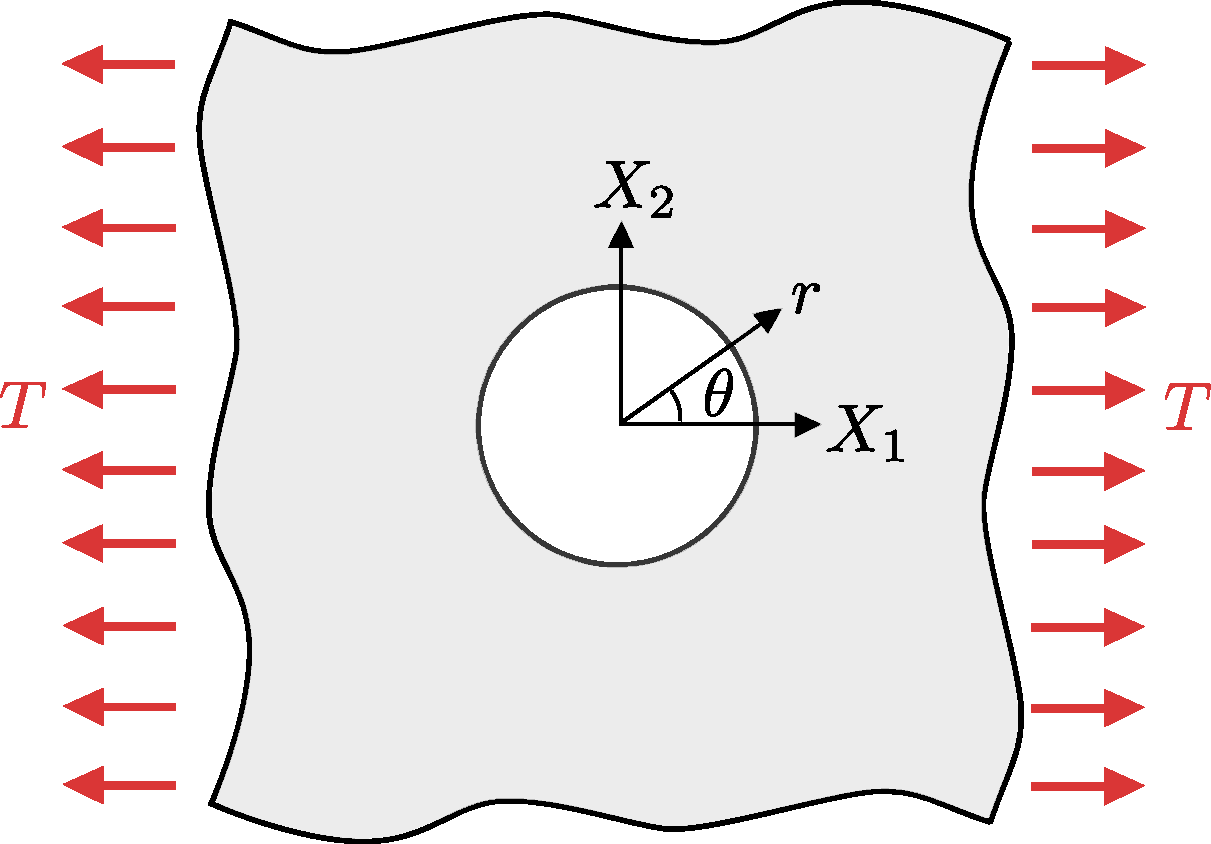
\includegraphics[width=4.0in]{figures/plate_with_hole.pdf}  \caption{Infinite plate with a circular hole placed in uniaxial tension.}
  \label{fig:plate_with_hole_problem}
\end{figure}
To demonstrate optimal convergence of the PEM for higher-order elements, we will choose to investigate the 2D elastostatics problem of an infinite plate with a circular hole in uniaxial tension (depicted in figure \ref{fig:plate_with_hole_problem}), for which there exist analytical solutions of the resulting displacement and stress fields (obtained from reference \cite{Wikiversity:17}):
\begin{equation}
  u_1 (r,\theta) = \frac{Ta}{8\mu} \left[ \frac{r}{a} (\kappa + 1) \cos \theta + \frac{2a}{r} ((1+\kappa) \cos \theta + \cos 3 \theta) - \frac{2a^3}{r^3} \cos 3 \theta \right]
\end{equation}
\begin{equation}
  u_2 (r,\theta) = \frac{Ta}{8\mu} \left[ \frac{r}{a} (\kappa - 3) \sin \theta + \frac{2a}{r} ((1-\kappa) \sin \theta + \sin 3 \theta) - \frac{2a^3}{r^3} \sin 3 \theta \right]
\end{equation}
\begin{equation}
  \sigma_{11} (r, \theta) = T - T \frac{a^2}{r^2} \bigg( \frac{3}{2} \cos 2 \theta + \cos 4 \theta \bigg) + T \frac{3a^4}{2r^4} \cos 4 \theta
\end{equation}
\begin{equation}
  \sigma_{22} (r, \theta) = - T \frac{a^2}{r^2} \bigg( \frac{1}{2} \cos 2 \theta - \cos 4 \theta \bigg) - T \frac{3a^4}{2r^4} \cos 4 \theta
\end{equation}
\begin{equation}
  \sigma_{12} (r, \theta) = - T \frac{a^2}{r^2} \bigg( \frac{1}{2} \sin 2 \theta + \sin 4 \theta \bigg) + T \frac{3a^4}{2r^4} \sin 4 \theta
\end{equation}
where $T$ is the far-field value of the applied tensile stress, $a$ is the radius of the circular hole centered at $r=0$, $\kappa = 4 - 3\nu$ (under plane-strain conditions), and $\nu$ and $\mu$ are the the Poisson's ratio and shear modulus of the material, respectively.

\begin{figure}[!h]
  \centering
  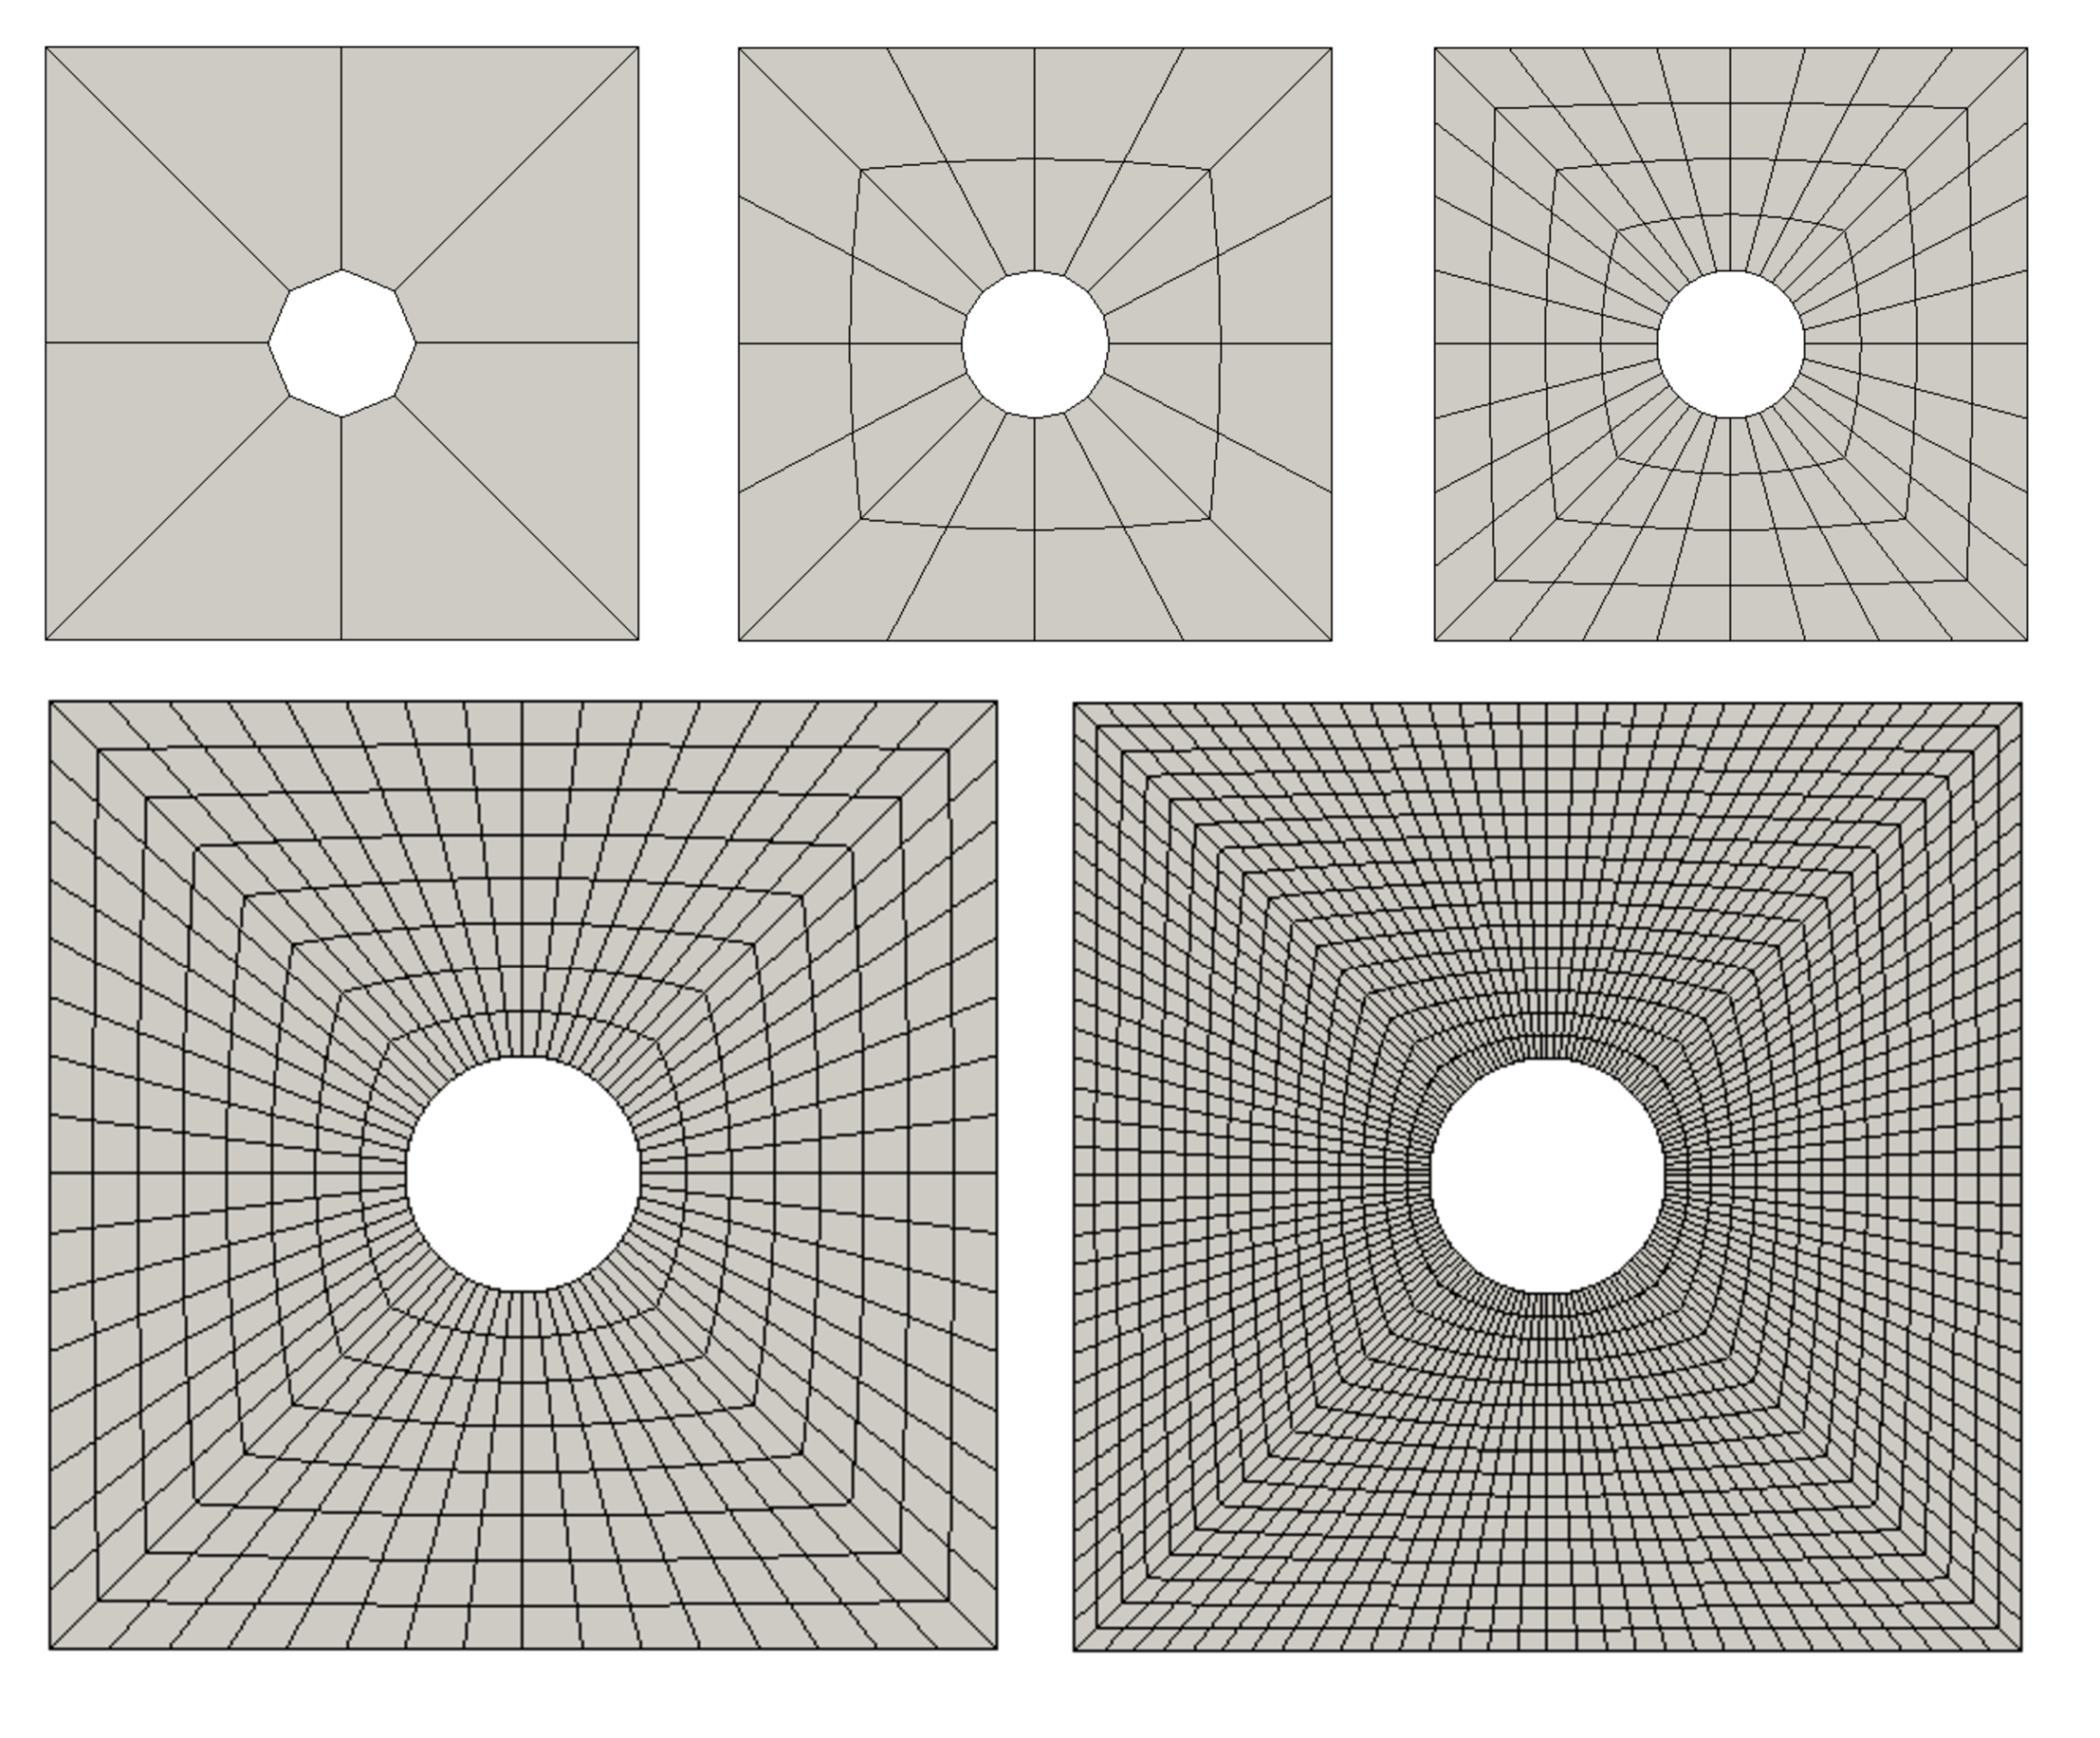
\includegraphics[width=6.0in]{figures/plate_with_hole_meshes.pdf}
  \caption{Quadrilateral meshes with varying levels of refinement.}
  \label{fig:plate_with_hole_meshes}
\end{figure}
A convergence study was carried out using a series of quadrilateral meshes with varying levels of refinement discretizing the restricted problem domain $X_i \in [ -1, +1]$ (see figure \ref{fig:plate_with_hole_meshes}.) The meshes consisted of either 4-node quadrilateral or 8-node serendipity quadrilateral elements, and employed either an isoparametric formulation, or a sufficiently high-order PEM formulation (i.e. $k=1$ for 4-node quadrilaterals, and $k=2$ for 8-node quadrilaterals.) Displacement boundary conditions were prescribed to be consistent with the exact solution on the restricted boundary. $L^2$ displacement error norms and $H^1$ energy error semi-norms were computed with reference to the exact solution, with the numerical results summarized in tables \ref{tab:l2_error}-\ref{tab:h1_rates}. The convergence rates in the $L^2$ and $H^1$ error norms are depicted in figures \ref{fig:l2_error} and \ref{fig:h1_error}, respectively.
\newpage
\begin{table}[!ht]
  \begin{center}
    \begin{tabular}{| c | c | c | c | c |}
    \hline
    $h$ & 4-node FEM & 4-node PEM & 8-node FEM & 8-node PEM \\ \hline
    1.2500 & 1.3133E-006 & 1.4901E-006 & 9.8369E-007 & 2.9990E-006 \\ \hline
    0.8006 & 6.9557E-007 & 9.8453E-007 & 4.8165E-007 & 1.3918E-006 \\ \hline
    0.4488 & 2.8755E-007 & 4.2859E-007 & 2.2034E-007 & 3.3673E-007 \\ \hline
    0.2371 & 1.0460E-007 & 1.3672E-007 & 8.1971E-008 & 4.8942E-008 \\ \hline
    0.1218 & 3.1430E-008 & 3.7296E-008 & 2.4628E-008 & 6.7201E-009 \\ \hline
    0.0617 & 8.3877E-009 & 9.5661E-009 & 6.5479E-009 & 1.6002E-009 \\
    \hline
    \end{tabular}
    \caption{Computed $L^2$ displacement error norms.}
    \vspace{-5pt}
    \label{tab:l2_error}
    \vspace{-25pt}
  \end{center}
\end{table}
\begin{table}[!ht]
  \begin{center}
    \begin{tabular}{| c | c | c | c | c |}
    \hline
    $h$ & 4-node FEM & 4-node PEM & 8-node FEM & 8-node PEM \\ \hline
    1.2500 &	-	&	-	&	-	&       -      \\ \hline
    0.8006 &	1.4265	&	0.9302	&	1.6028	&	1.7230 \\ \hline
    0.4488 &	1.5262	&	1.4369	&	1.3512	&	2.4518 \\ \hline
    0.2371 &	1.5848	&	1.7906	&	1.5496	&	3.0225 \\ \hline
    0.1218 &	1.8051	&	1.9502	&	1.8053	&	2.9808 \\ \hline
    0.0617 &	1.9424	&	2.0007	&	1.9479	&	2.1100 \\
    \hline
    \end{tabular}
    \caption{Computed $L^2$ displacement error norm convergence rates.}
    \vspace{-5pt}
    \label{tab:l2_rates}
    \vspace{-25pt}
  \end{center}
\end{table}
\begin{table}[!ht]
  \begin{center}
    \begin{tabular}{| c | c | c | c | c |}
    \hline
    $h$ & 4-node FEM & 4-node PEM & 8-node FEM & 8-node PEM \\ \hline
    1.2500 & 2.1468E-001 & 2.8913E-001 & 1.8275E-001 & 5.3700E-001 \\ \hline
    0.8006 & 1.8622E-001 & 2.5620E-001 & 1.5959E-001 & 3.0529E-001 \\ \hline
    0.4488 & 1.3786E-001 & 1.7930E-001 & 1.2495E-001 & 1.5310E-001 \\ \hline
    0.2371 & 9.2075E-002 & 1.1251E-001 & 7.9144E-002 & 5.8671E-002 \\ \hline
    0.1218 & 5.2124E-002 & 6.2223E-002 & 4.2868E-002 & 1.5541E-002 \\ \hline
    0.0617 & 2.7048E-002 & 3.2135E-002 & 2.1789E-002 & 3.3672E-003 \\
    \hline
    \end{tabular}
    \caption{Computed $H^1$ energy error semi-norms.}
    \vspace{-5pt}
    \label{tab:h1_error}
    \vspace{-25pt}
  \end{center}
\end{table}
\begin{table}[!ht]
  \begin{center}
    \begin{tabular}{| c | c | c | c | c |}
    \hline
    $h$ & 4-node FEM & 4-node PEM & 8-node FEM & 8-node PEM \\ \hline
    1.2500 &	-	&	-	&	-	&       -      \\ \hline
    0.8006 &	0.3192	&	0.2714	&	0.3042	&	1.2675 \\ \hline
    0.4488 &	0.5195	&	0.6166	&	0.4228	&	1.1924 \\ \hline
    0.2371 &	0.6326	&	0.7303	&	0.7156	&	1.5031 \\ \hline
    0.1218 &	0.8542	&	0.8892	&	0.9205	&	1.9944 \\ \hline
    0.0617 &	0.9646	&	0.9716	&	0.9950	&	2.2488 \\
    \hline
    \end{tabular}
    \caption{Computed $H^1$ energy error semi-norm convergence rates.}
    \vspace{-5pt}
    \label{tab:h1_rates}
    \vspace{-25pt}
  \end{center}
\end{table}
\begin{figure}[!h]
  \centering
  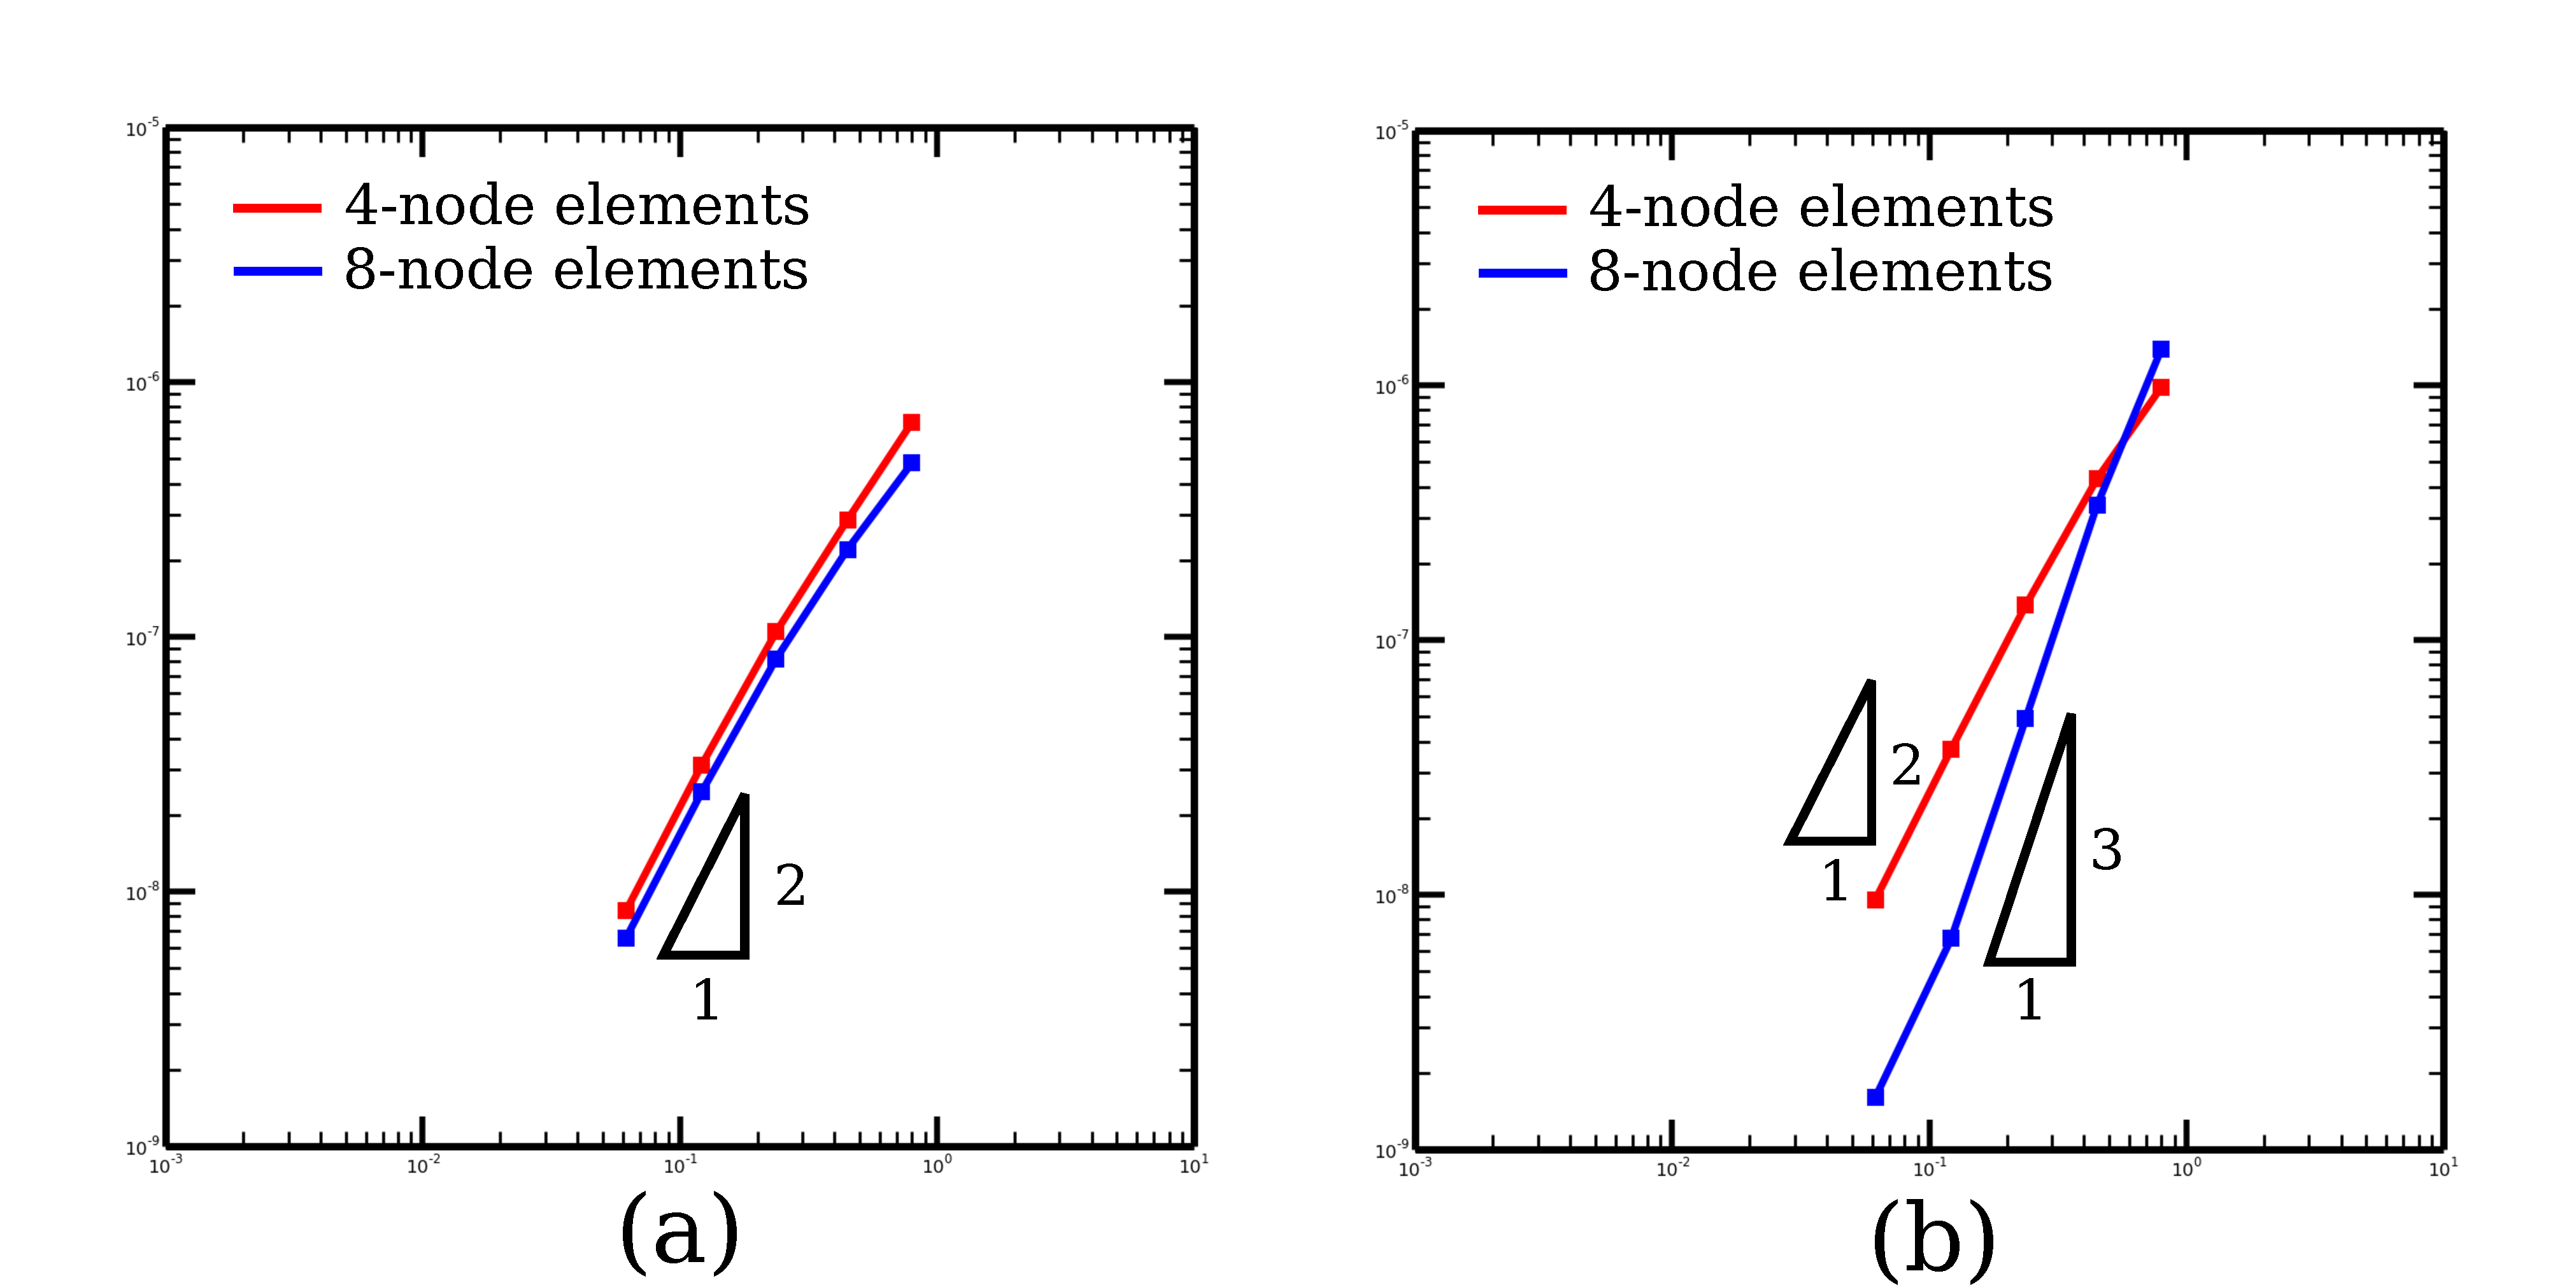
\includegraphics[width=6.0in]{figures/l2_error_plot.pdf}
  \caption{$L^2$ error convergence plots for (a) FEM and (b) PEM formulations.}
  \label{fig:l2_error}
  \vspace{-10pt}
\end{figure}

\begin{figure}[!h]
  \centering
  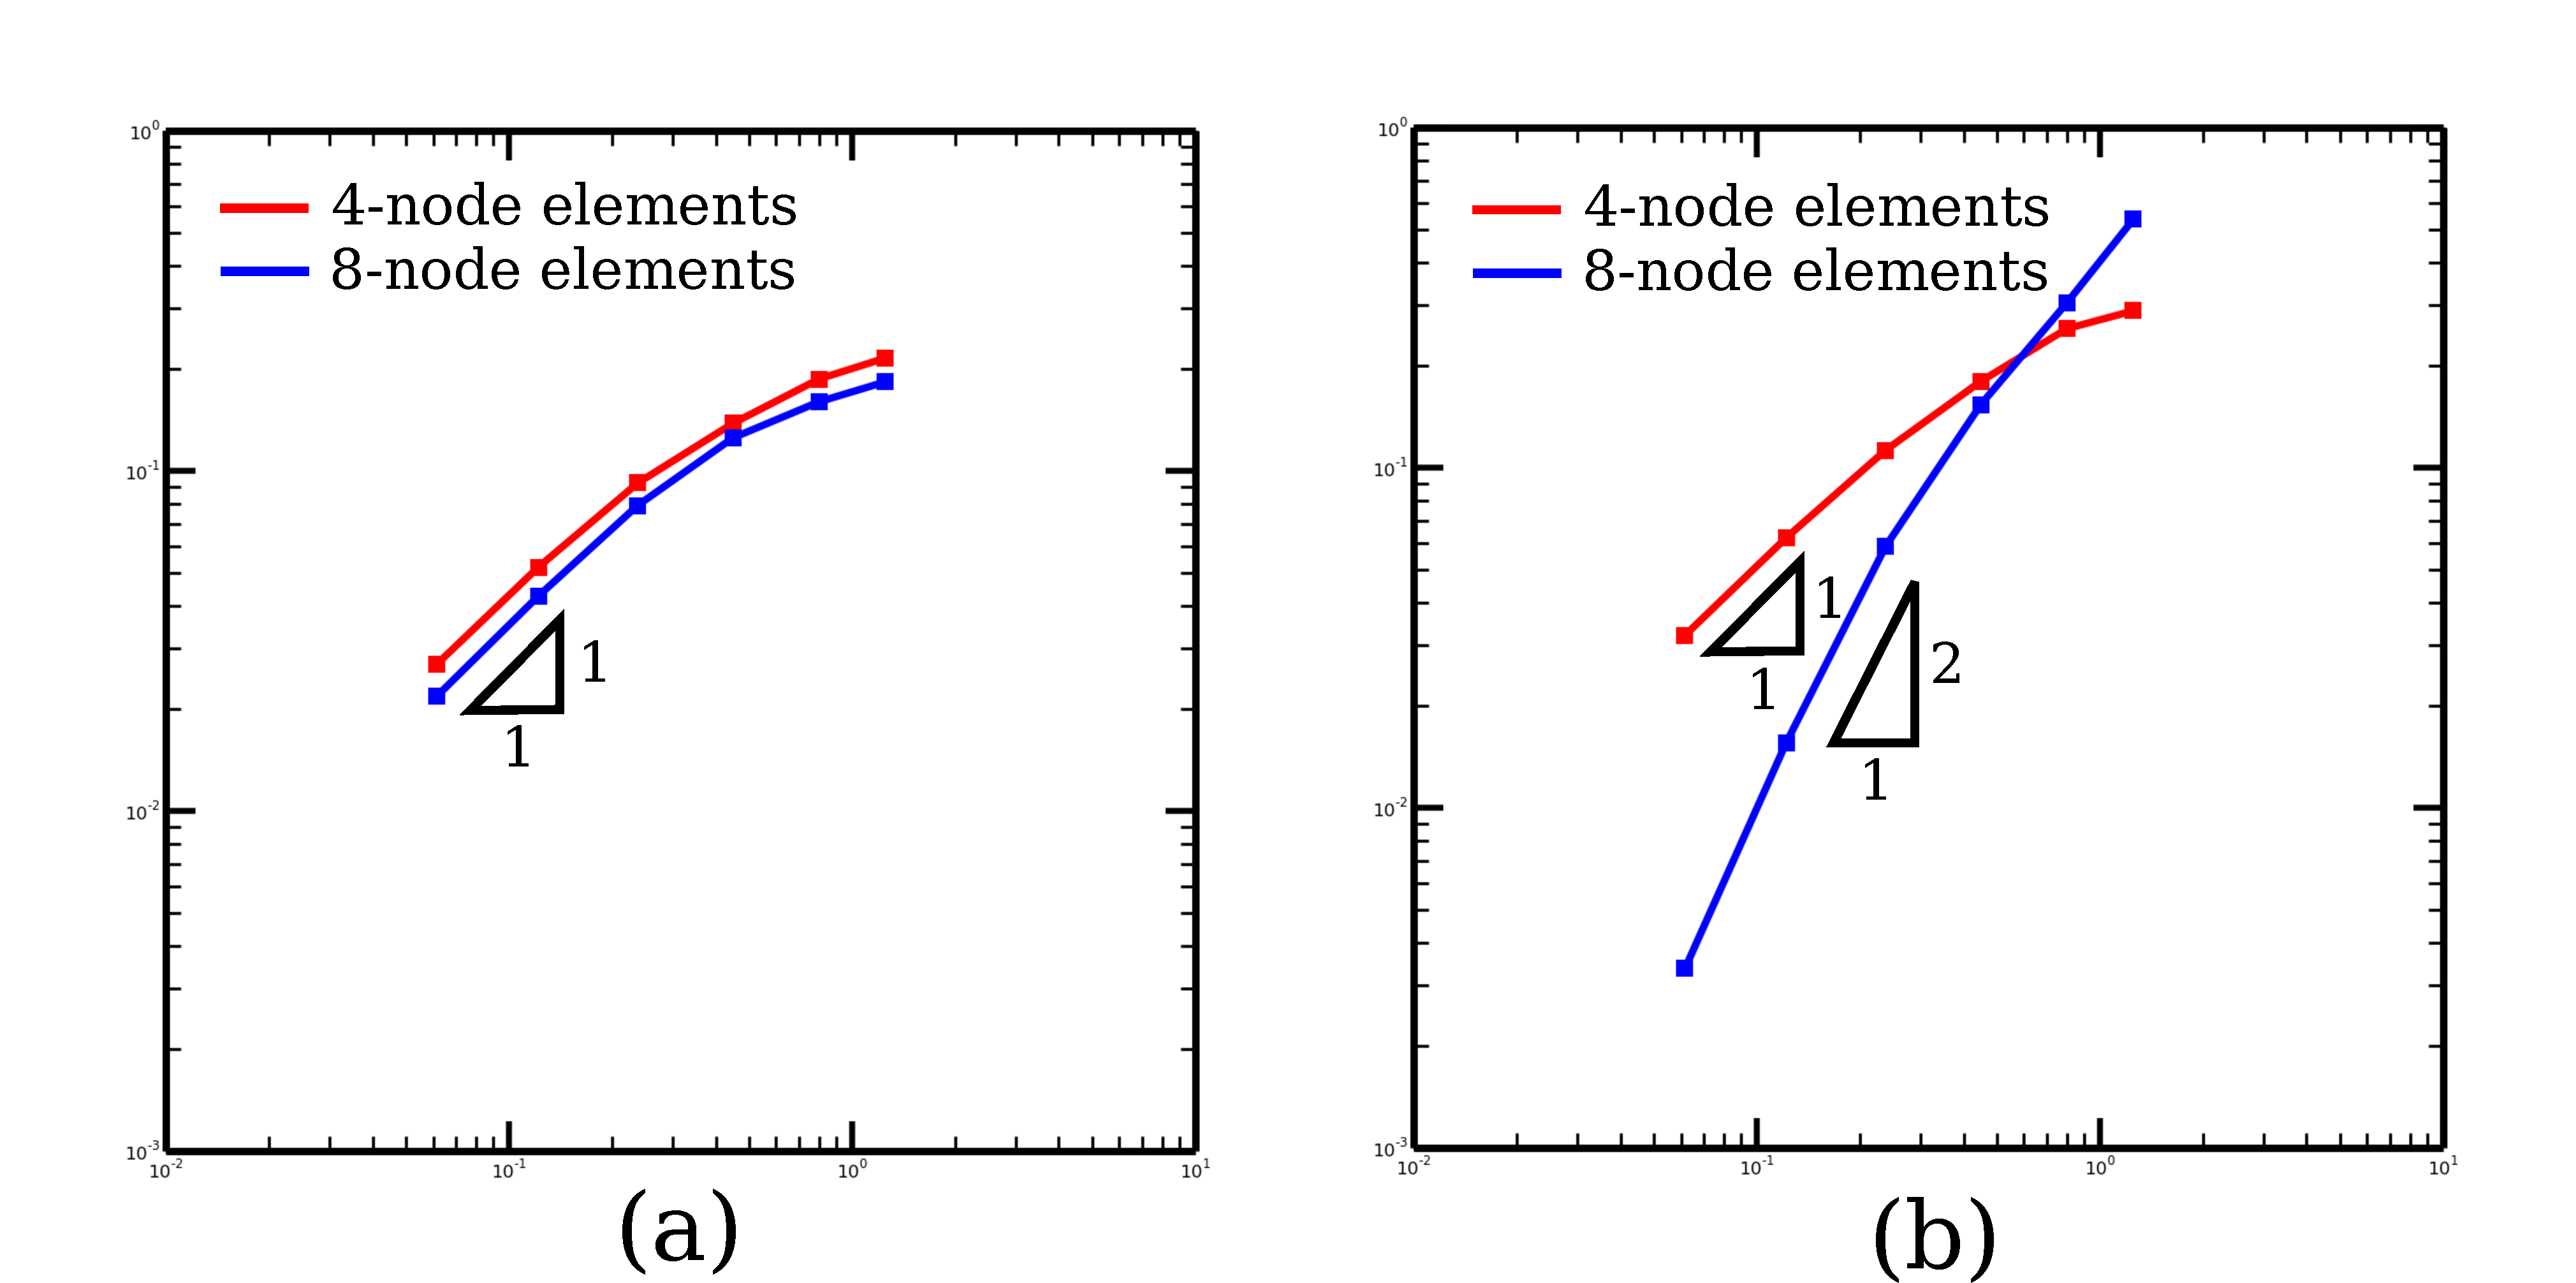
\includegraphics[width=6.0in]{figures/h1_error_plot.pdf}
  \caption{$H^1$ error convergence plots for (a) FEM and (b) PEM formulations.}
  \label{fig:h1_error}
\end{figure}

A number of observations should be made regarding the resulting data. In particular, it is worthwhile to note that part of the incurred solution error may be attributable to the inexact representation of the problem geometry, especially for the coarse meshes. This may in part explain why the observed convergence rates are lower at coarser levels of refinement, but approach the expected rates as the mesh is further refined.

Additionally, we remark that isoparametric serendipity quadrilateral elements converge at sub-optimal rates if the elements are distorted in a non-affine fashion (as is the case for our meshes). This is an altogether expected result, and has been discussed in references \cite{Arnold:01} and \cite{Arnold:02}.

Conversely, we observe that the PEM quadrilateral elements converge at the optimal rates in both the $L^2$ and $H^1$ error norms, as we would hope.

Further work will seek to investigate the measured error and convergence rates of the PEM when the elements take on arbitrary shape, and for a variety of different formulations and penalization parameter settings.

\section{Parameter Sensitivity Analysis}

\section{Computational Efficiency}
\subsection{Performance Comparison}

\section{Resistance to Locking Phenomena}

\subsection*{Twisting Annulus}

Consider an incompressible elastic annulus whose inner radius at $r = R_i$ is fixed, and whose outer radius $r = R_o$ rigidly rotates at an angular velocity of $\Phi$. The radially symmetric displacement boundary conditions for this motion are described by
\begin{equation}
	u_r (R_i,t) = u_r (R_o,t) = 0, \quad u_z (R_i,t) = u_z (R_o,t) = 0,
\end{equation}
\begin{equation}
	u_\theta (R_i,t) = 0, \quad u_\theta (R_o,t) = R_o \, \Phi \, t,
\end{equation}
for $t \geq 0$.

The elastic material is characterized by a linear hypoelastic material model of grade zero, obeying
\begin{equation}
  \dot{\boldsymbol{\sigma}} = \mathbb{C} : \mathbf{D} + \mathbf{W} \boldsymbol{\sigma} - \boldsymbol{\sigma} \mathbf{W},
\end{equation}

\subsubsection*{Exact Solution}

An exact solution for the aforementioned problem may be obtained by considering the stress divergence equations in cylindrical polar coordinates:
\begin{equation}
  \nabla \cdot \boldsymbol{\sigma} = \left\{ \begin{array}{c} \frac{\partial \sigma_{rr}}{\partial r} + \frac{\sigma_{rr}}{r} + \frac{1}{r} \frac{\partial \sigma_{\theta r}}{\partial \theta} + \frac{\partial \sigma_{z r}}{\partial z} - \frac{\sigma_{\theta \theta}}{r} \\
    \frac{1}{r} \frac{\partial \sigma_{\theta \theta}}{\partial \theta} + \frac{\partial \sigma_{r\theta}}{\partial r} + \frac{\sigma_{r\theta}}{r} + \frac{\sigma_{\theta r}}{r} + \frac{\partial \sigma_{z \theta}}{\partial z} \\
    \frac{\partial \sigma_{z z}}{\partial z} + \frac{\partial \sigma_{r z}}{\partial r} + \frac{\sigma_{r z}}{r} + \frac{1}{r} \frac{\partial \sigma_{\theta z}}{\partial \theta} \end{array} \right\} = \mathbf{0}.
\end{equation}
By the assumptions of plane strain and axisymmetry, we rationalize that $\boldsymbol{\sigma} (r)$ is a function of $r$, alone, and therefore,
\begin{equation}
  \nabla \cdot \boldsymbol{\sigma} = \left\{ \begin{array}{c} \frac{\partial \sigma_{rr}}{\partial r} + \frac{\sigma_{rr} - \sigma_{\theta \theta}}{r} \\
    \frac{\partial \sigma_{r\theta}}{\partial r} + \frac{2 \sigma_{r\theta}}{r} \\
    \frac{\partial \sigma_{r z}}{\partial r} + \frac{\sigma_{r z}}{r} \end{array} \right\} = \mathbf{0}.
\end{equation}
Furthermore, by the assumptions of plane strain, we observe that $\sigma_{rz} = 0$ and $\sigma_{\theta z} = 0$. Additionally, if we impose the incompressibility condition $\nabla \cdot \mathbf{v} = \text{tr} (\mathbf{D}) = 0$, we find that
\begin{equation}
  \text{tr} (\dot{\boldsymbol{\sigma}}) = 0 \, \Rightarrow \, \text{tr} (\boldsymbol{\sigma}) = 0 \, \forall t.
\end{equation}
The deformation necessitates that $\sigma_{zz} = 0$, and therefore $\sigma_{\theta \theta} = - \sigma_{rr}$. Consequently, we are left with 2 governing differential equations for $\sigma_{rr}$ and $\sigma_{r \theta}$:
\begin{equation}
  \frac{\partial \sigma_{rr}}{\partial r} + \frac{2 \sigma_{rr}}{r} = 0, \quad \frac{\partial \sigma_{r\theta}}{\partial r} + \frac{2 \sigma_{r\theta}}{r} = 0,
\end{equation}
whose solutions are of the form
\begin{equation}
  \sigma_{rr} = \frac{a}{r^2}, \quad \sigma_{r\theta} = \frac{b}{r^2}.
\end{equation}
Consequently,
\begin{equation}
  \left\{ \begin{array}{c} \sigma_{rr} \\ \sigma_{\theta \theta} \\ \sigma_{r \theta} \end{array} \right\} = r^{-2} \left\{ \begin{array}{c} +a \\ -a \\ b \end{array} \right\}.
\end{equation}

Under the assumption of incompressibility, we may characterize the deformation via the velocity field $v_r = 0$, $v_z = 0$, and $v_\theta (r) = r \dot{\phi}(r)$, yielding the velocity gradient (in cylindrical polar coordinates):
\begin{equation}
  \mathbf{L} = \nabla \mathbf{v} = \left[ \begin{array}{ccc} v_{r,r} & v_{r,\theta}/r-v_\theta /r & v_{r,z} \\
      v_{\theta,r} & v_{\theta,\theta}/r + v_r /r & v_{\theta,z} \\
      v_{z,r} & v_{z,\theta} /r & v_{z,z} \end{array} \right] = 
  \left[ \begin{array}{ccc} 0 & -\dot{\phi} & 0 \\
      \dot{\phi} + r \dot{\phi}_{,r} & 0 & 0 \\
      0 & 0 & 0 \end{array} \right],
\end{equation}
and the corresponding rate of deformation and spin tensors:
\begin{equation}
  \mathbf{D} = \frac{r \dot{\phi}_{,r}}{2} \left[ \begin{array}{ccc} 0 & 1 & 0 \\
      1 & 0 & 0 \\
      0 & 0 & 0 \end{array} \right], \quad \mathbf{W} = 
  \frac{2 \dot{\phi} + r \dot{\phi}_{,r}}{2} \left[ \begin{array}{ccc} 0 & - 1 & 0 \\
      1 & 0 & 0 \\
      0 & 0 & 0 \end{array} \right].
\end{equation}
The resulting stress rate equations are
\begin{equation}
  \left\{ \begin{array}{c} \dot{\sigma}_{rr} \\ \dot{\sigma}_{\theta \theta} \\ \dot{\sigma}_{r \theta} \end{array} \right\} = \left\{ \begin{array}{c} 0 \\ 0 \\ \mu r \dot{\phi}_{,r} \end{array} \right\} + 
  (2 \dot{\phi} + r \dot{\phi}_{,r}) \left\{ \begin{array}{c} - \sigma_{r \theta} \\ \sigma_{r \theta} \\ \sigma_{rr} \end{array} \right\},
\end{equation}
or
\begin{equation}
  \left\{ \begin{array}{c} \dot{a} \\ \dot{b} \end{array} \right\} = \left\{ \begin{array}{c} 0 \\ \mu r^3 \dot{\phi}_{,r} \end{array} \right\} + (2 \dot{\phi} + r \dot{\phi}_{,r}) \left[ \begin{array}{cc} 0 & -1 \\ 1 & 0 \end{array} \right] \left\{ \begin{array}{c} a \\ b \end{array} \right\},
\end{equation}
which must be valid $\forall r, \, t$. If we assume that $\dot{\phi} = f(r)$ is a function of $r$ (and not of $t$), then we obtain the condition
\begin{equation}
  3 f_{,r} + r f_{,rr} = 0,
\end{equation}
implying $f_{,r} = B r^{-3}$, and $\phi (r, t) = (A - B r^{-2} / 2)t$, thus
\begin{equation}
  \left\{ \begin{array}{c} \dot{a} \\ \dot{b} \end{array} \right\} = \left\{ \begin{array}{c} 0 \\ \mu B \end{array} \right\} + 2 A \left[ \begin{array}{cc} 0 & -1 \\ 1 & 0 \end{array} \right] \left\{ \begin{array}{c} a \\ b \end{array} \right\},
\end{equation}
and
\begin{equation}
  a(t) = - \frac{\mu B}{2 A} - C_2 \sin (2 A t) + C_1 \cos (2 A t),
\end{equation}
\begin{equation}
  b(t) = C_1 \sin (2 A t) + C_2 \cos (2 A t).
\end{equation}
Imposing the initial conditions $a(0) = b(0) = 0$ results in:
\begin{equation}
  a(t) = \frac{\mu B}{2 A} \left[ \cos (2 A t) - 1 \right], \quad b(t) = \frac{\mu B}{2 A} \sin (2 A t).
\end{equation}
Imposing the boundary conditions $\phi(R_i,t) = 0 \, \, \forall t$, $\phi(R_o,t) = \Phi \, t \, \, \forall t$ yields:
\begin{equation}
  A = \frac{\Phi R_i^{-2}}{R_i^{-2} - R_o^{-2}}, \quad B = \frac{2 \Phi}{R_i^{-2} - R_o^{-2}}.
\end{equation}

The final analytical solution for the displacement and stress fields is presented below:
\begin{equation}
  u_r = 0, \quad u_\theta = r \Phi \frac{R_i^{-2} - r^{-2}}{R_i^{-2} - R_o^{-2}} t, \quad u_z = 0,
\end{equation}
\begin{equation}
  \sigma_{rr} = - \sigma_{\theta \theta} = \mu \frac{r^{-2}}{R_i^{-2}} \left[ \cos \left( 2 \frac{\Phi R_i^{-2}}{R_i^{-2} - R_o^{-2}} t \right) - 1 \right],
\end{equation}
\begin{equation}
  \sigma_{r \theta} = \mu \frac{r^{-2}}{R_i^{-2}} \sin \left( 2 \frac{\Phi R_i^{-2}}{R_i^{-2} - R_o^{-2}} t \right).
\end{equation}
\chapter{Conclusions and Future Work}
%
Evaluate the efficacy of the proposed formulations within the presented context. Assess whether there really is a silver bullet to the locking problem, or if we can expect for locking to be an inherrent issue with any numerical approximation method.

Describe the nature of future work that will be done in this area of research.


\appendix

\chapter{An Exact Solution for the Incompressible Twisting Annulus Problem}

An exact solution for the twisting annulus problem described in chapter \ref{ch:results} may be obtained by considering the stress divergence equations in cylindrical polar coordinates:
\begin{equation}
  \nabla \cdot \boldsymbol{\sigma} = \left\{ \begin{array}{c} \frac{\partial \sigma_{rr}}{\partial r} + \frac{\sigma_{rr}}{r} + \frac{1}{r} \frac{\partial \sigma_{\theta r}}{\partial \theta} + \frac{\partial \sigma_{z r}}{\partial z} - \frac{\sigma_{\theta \theta}}{r} \\
    \frac{1}{r} \frac{\partial \sigma_{\theta \theta}}{\partial \theta} + \frac{\partial \sigma_{r\theta}}{\partial r} + \frac{\sigma_{r\theta}}{r} + \frac{\sigma_{\theta r}}{r} + \frac{\partial \sigma_{z \theta}}{\partial z} \\
    \frac{\partial \sigma_{z z}}{\partial z} + \frac{\partial \sigma_{r z}}{\partial r} + \frac{\sigma_{r z}}{r} + \frac{1}{r} \frac{\partial \sigma_{\theta z}}{\partial \theta} \end{array} \right\} = \mathbf{0}.
\end{equation}
By the assumptions of plane strain and axisymmetry, it is rationalized that $\boldsymbol{\sigma} (r)$ must be a function of $r$, alone. Therefore:
\begin{equation}
  \nabla \cdot \boldsymbol{\sigma} = \left\{ \begin{array}{c} \frac{\partial \sigma_{rr}}{\partial r} + \frac{\sigma_{rr} - \sigma_{\theta \theta}}{r} \\
    \frac{\partial \sigma_{r\theta}}{\partial r} + \frac{2 \sigma_{r\theta}}{r} \\
    \frac{\partial \sigma_{r z}}{\partial r} + \frac{\sigma_{r z}}{r} \end{array} \right\} = \mathbf{0}.
\end{equation}
Furthermore, by the assumptions of plane strain, it is observed that $\sigma_{rz} = 0$ and $\sigma_{\theta z} = 0$. Additionally, imposing the incompressibility condition $\nabla \cdot \mathbf{v} = \text{tr} (\mathbf{D}) = 0$:
\begin{equation}
  \text{tr} (\dot{\boldsymbol{\sigma}}) = 0 \, \Rightarrow \, \text{tr} (\boldsymbol{\sigma}) = 0 \, \forall t.
\end{equation}
Suppose that $p = \sigma_{zz} = 0$, and therefore $\sigma_{\theta \theta} = - \sigma_{rr}$. This yields 2 governing differential equations for $\sigma_{rr}$ and $\sigma_{r \theta}$:
\begin{equation}
  \frac{\partial \sigma_{rr}}{\partial r} + \frac{2 \sigma_{rr}}{r} = 0, \quad \frac{\partial \sigma_{r\theta}}{\partial r} + \frac{2 \sigma_{r\theta}}{r} = 0,
\end{equation}
whose solutions are of the form
\begin{equation}
  \sigma_{rr} = \frac{\sigma}{r^2}, \quad \sigma_{r\theta} = \frac{\tau}{r^2},
\end{equation}
where $\sigma(t)$ and $\tau(t)$ are independent functions of time. Consequently,
\begin{equation}
  \left\{ \begin{array}{c} \sigma_{rr} \\ \sigma_{\theta \theta} \\ \sigma_{r \theta} \end{array} \right\} = r^{-2} \left\{ \begin{array}{c} +\sigma \\ -\sigma \\ \tau \end{array} \right\}.
\end{equation}

Under the assumption of incompressibility, the velocity field is $v_r = 0$, $v_z = 0$, and $v_\theta (r) = r \dot{\phi}(r)$, for some $\phi(r,t)$. The velocity gradient (in cylindrical polar coordinates) is written:
\begin{equation}
  \mathbf{L} = \nabla \mathbf{v} = \left[ \begin{array}{ccc} v_{r,r} & v_{r,\theta}/r-v_\theta /r & v_{r,z} \\
      v_{\theta,r} & v_{\theta,\theta}/r + v_r /r & v_{\theta,z} \\
      v_{z,r} & v_{z,\theta} /r & v_{z,z} \end{array} \right] = 
  \left[ \begin{array}{ccc} 0 & -\dot{\phi} & 0 \\
      \dot{\phi} + r \dot{\phi}_{,r} & 0 & 0 \\
      0 & 0 & 0 \end{array} \right].
\end{equation}
The corresponding rate of deformation and spin tensors are:
\begin{equation}
  \mathbf{D} = \frac{r \dot{\phi}_{,r}}{2} \left[ \begin{array}{ccc} 0 & +1 & 0 \\
      +1 & 0 & 0 \\
      0 & 0 & 0 \end{array} \right], \quad \mathbf{W} = 
  \frac{2 \dot{\phi} + r \dot{\phi}_{,r}}{2} \left[ \begin{array}{ccc} 0 & - 1 & 0 \\
      +1 & 0 & 0 \\
      0 & 0 & 0 \end{array} \right].
\end{equation}
The stress rate equations resulting from $\dot{\boldsymbol{\sigma}} = \mathbb{C} : \mathbf{D} + \mathbf{W} \boldsymbol{\sigma} - \boldsymbol{\sigma} \mathbf{W}$ are
\begin{equation}
  \left\{ \begin{array}{c} \dot{\sigma}_{rr} \\ \dot{\sigma}_{\theta \theta} \\ \dot{\sigma}_{r \theta} \end{array} \right\} = \left\{ \begin{array}{c} 0 \\ 0 \\ \mu r \dot{\phi}_{,r} \end{array} \right\} + 
  (2 \dot{\phi} + r \dot{\phi}_{,r}) \left\{ \begin{array}{c} - \sigma_{r \theta} \\ \sigma_{r \theta} \\ \sigma_{rr} \end{array} \right\},
\end{equation}
or (in terms of $\sigma$, $\tau$):
\begin{equation}
  \left\{ \begin{array}{c} \dot{\sigma} \\ \dot{\tau} \end{array} \right\} = \left\{ \begin{array}{c} 0 \\ \mu r^3 \dot{\phi}_{,r} \end{array} \right\} + (2 \dot{\phi} + r \dot{\phi}_{,r}) \left[ \begin{array}{cc} 0 & -1 \\ 1 & 0 \end{array} \right] \left\{ \begin{array}{c} \sigma \\ \tau \end{array} \right\},
\end{equation}
which must be valid for all $r, \, t$. Assume that $\dot{\phi}(r)$ is a function of $r$ (and not of $t$), corresponding to a steady rate of deformation. By recognizing that $\sigma_{,r} = \tau_{,r} = 0$, one obtains the condition
\begin{equation}
  3 \dot{\phi}_{,r} + r \dot{\phi}_{,rr} = 0,
\end{equation}
implying $\dot{\phi}_{,r} = B r^{-3}$, and $\phi (r, t) = (A - B r^{-2} / 2)t$. Thus
\begin{equation}
  \left\{ \begin{array}{c} \dot{\sigma} \\ \dot{\tau} \end{array} \right\} = \left\{ \begin{array}{c} 0 \\ \mu B \end{array} \right\} + 2 A \left[ \begin{array}{cc} 0 & -1 \\ 1 & 0 \end{array} \right] \left\{ \begin{array}{c} \sigma \\ \tau \end{array} \right\},
\end{equation}
and
\begin{equation}
  \sigma(t) = - \frac{\mu B}{2 A} - C_2 \sin (2 A t) + C_1 \cos (2 A t),
\end{equation}
\begin{equation}
  \tau(t) = C_1 \sin (2 A t) + C_2 \cos (2 A t).
\end{equation}
Imposing the initial conditions $\sigma(0) = \tau(0) = 0$ results in:
\begin{equation}
  \sigma(t) = \frac{\mu B}{2 A} \left[ \cos (2 A t) - 1 \right], \quad \tau(t) = \frac{\mu B}{2 A} \sin (2 A t).
\end{equation}
Imposing the boundary conditions $\phi(R_i,t) = 0 \, \, \forall t$, $\phi(R_o,t) = \Phi \, t \, \, \forall t$ yields:
\begin{equation}
  A = \frac{R_o^{2}}{R_o^{2} - R_i^{2}} \Phi, \quad B = 2 \frac{R_o^{2} R_i^{2}}{R_o^{2} - R_i^{2}} \Phi.
\end{equation}
The final analytical solutions for the displacement and stress fields are:
\begin{equation}
  u_r = u_z = 0, \quad u_\theta = \frac{R_o^2}{r} \frac{r^2 - R_i^2}{R_o^{2} - R_i^{2}} \Phi t,
\end{equation}
\begin{equation}
  \sigma_{rr} = - \sigma_{\theta \theta} = \mu \frac{R_i^{2}}{r^{2}} \left[ \cos \left( 2 \frac{R_o^{2}}{R_o^{2} - R_i^{2}} \Phi t \right) - 1 \right], \quad \sigma_{r \theta} = \mu \frac{R_i^{2}}{r^{2}} \sin \left( 2 \frac{R_o^{2}}{R_o^{2} - R_i^{2}} \Phi t \right).
\end{equation}
According to \cite{Brannon:11}, the above solution for $\sigma_{r \theta}$ is also valid for compressible elastic materials.

\bibliography{bibliography}

% The UMI abstract uses square brackets!
\UMIabstract[The abstract that is submitted to UMI must be formatted as shown in the example here. The body of the abstract cannot exceed 350 words. It should be in typewritten form, double-spaced, and on bond paper. It is important to write an abstract that gives a clear description of the content and major divisions of the dissertation, since UMI will publish the abstract exactly as submitted. Students completing their requirements under Plan A should provide extra copies of the typed summary for use by the dissertation committee during the examination.

The abstract that is submitted to UMI must be formatted as shown in the example here. The body of the abstract cannot exceed 350 words. It should be in typewritten form, double-spaced, and on bond paper. It is important to write an abstract that gives a clear description of the content and major divisions of the dissertation, since UMI will publish the abstract exactly as submitted. Students completing their requirements under Plan A should provide extra copies of the typed summary for use by the dissertation committee during the examination.

The abstract that is submitted to UMI must be formatted as shown in the example here. The body of the abstract cannot exceed 350 words. It should be in typewritten form, double-spaced, and on bond paper. It is important to write an abstract that gives a clear description of the content and major divisions of the dissertation, since UMI will publish the abstract exactly as submitted. Students completing their requirements under Plan A should provide extra copies of the typed summary for use by the dissertation committee during the examination.

The abstract that is submitted to UMI must be formatted as shown in the example here. The body of the abstract cannot exceed 350 words. It should be in typewritten form, double-spaced, and on bond paper. It is important to write an abstract that gives a clear description of the content and major divisions of the dissertation, since UMI will publish the abstract exactly as submitted. Students completing their requirements under Plan A should provide extra copies of the typed summary for use by the dissertation committee during the examination.]

\end{document} 
